\documentclass{report}
\usepackage[utf8]{inputenc}
\usepackage{amsmath}
\usepackage{amsthm}
\newtheorem{theorem}{Theorem}
\usepackage{array}
\usepackage{braket}
\usepackage{mathpartir}
\usepackage{framed}
\usepackage{graphicx}
\usepackage{geometry}
\usepackage{stmaryrd}
\usepackage{tikz}
\usepackage{amssymb} % Package for \Box
\usepackage{url}
\usepackage{comment}
\usepackage{hyperref}
%\usepackage{upgreek}
\usepackage{tikz}
\usepackage[square,super,sort]{natbib}
\usepackage[shortlabels]{enumitem}
\usetikzlibrary{shapes.geometric,arrows.meta}
\usepackage{longtable} % For tables spanning multiple pages
\usepackage{multirow}
\usepackage{hhline}
\usepackage{listings}
\usepackage{tcolorbox}
\usepackage{booktabs}
\newtheorem{lemma}{Lemma}
\newtheorem{corollary}{Corollary}
\DeclareMathOperator{\Var}{var}
\allowdisplaybreaks
\newtheorem{definition}{Definition}[section]
\setlength{\arrayrulewidth}{1.2pt} % Set line width to 1.2pt
\hypersetup{
  colorlinks=true,
  citecolor=blue,
  urlcolor=blue,
  linkcolor=blue,
  hypertexnames=false,
  bookmarksdepth=1
}
\geometry{a4paper,scale=0.9}
\DeclareFontShape{OT1}{cmr}{bx}{sc}{<->ssub*cmr/bx/n}{}
\AtBeginDocument{%
  \global\hbadness=10000
  \global\vbadness=10000
  \global\hfuzz=\maxdimen
  \global\vfuzz=\maxdimen
  \global\overfullrule=0pt
}

\newtheoremstyle{defn_style}      % Name
  {}%                             % Space above
  {}%                             % Space below
  {}%                             % Body font
  {}%                             % Indent amount
  {\bfseries}%                    % Theorem head font
  {.}%                            % Punctuation after theorem head
  { }%                            % Space after theorem head, ' ', or \newline
  {\thmname{#1}\thmnumber{#2}\thmnote{ (#3)}} % Theorem head spec (can be left empty, meaning `normal')

\theoremstyle{defn_style}
\newtheorem{defn}{Definition}[section]
\newtheorem{example}{Example}[section]
\newtheorem{pro}{Proposition}[section]
\newtheorem{pros}{Properties}[section]
\newtheorem{lem}{Lemma}[section]
\newtheorem{thm}{Theorem}[section]

\newcommand{\op}[2]{\ket{#1}\!\bra{#2}}
\newcommand{\opp}[3]{\ket{#1}\!_{#3}\!\bra{#2}}
\newcommand{\sem}[1]{\llbracket #1 \rrbracket}
\newcommand{\asteq}{\mathrel{*}=}
\newcommand{\supp}{\textup{supp}}
\newcommand{\spn}{span}
\newcommand{\tr}{\textup{tr}}
\newcommand{\prj}{\textup{proj}}
\providecommand{\res}{\mathsf{res}}
\providecommand{\rel}{\mathsf{rel}}
\providecommand{\Live}{\operatorname{Live}}
\providecommand{\Fresh}{\operatorname{Fresh}}
\providecommand{\AllocOK}{\operatorname{AllocOK}}
\providecommand{\Own}{\operatorname{Own}}
\providecommand{\Req}{\operatorname{Req}_{\mathsf{res}}}
\providecommand{\acc}{\operatorname{acc}}
\providecommand{\upd}{\operatorname{upd}}
\providecommand{\Obs}{\operatorname{Obs}}
\providecommand{\susp}{\mathsf{susp}}
\providecommand{\HopLC}[1]{\mathsf{LC}^{[#1]}}
\providecommand{\HopBB}[1]{\mathsf{BB}^{[#1]}}
\providecommand{\Out}{\mathsf{Out}}
\providecommand{\term}{\mathsf{term}}

\newcommand{\SKIP}{\ensuremath{\mathbf{skip}}}
\newcommand{\IF}{\ensuremath{\mathbf{if}}}
\newcommand{\THEN}{\ensuremath{\mathbf{then}}}
\newcommand{\ELSE}{\ensuremath{\mathbf{else}}}
\newcommand{\FI}{\ensuremath{\mathbf{fi}}}
\newcommand{\WHILE}{\ensuremath{\mathbf{while}}}
\newcommand{\MEAS}{\ensuremath{\mathbf{meas}}}
\newcommand{\DO}{\ensuremath{\mathbf{do}}}
\newcommand{\OD}{\ensuremath{\mathbf{od}}}
\newcommand{\FOR}{\ensuremath{\mathbf{for}}}
\newcommand{\ERR}{\ensuremath{\mathbf{error}}}
\newcommand{\ASSERT}{\ensuremath{\mathbf{assert}}}
\newcommand{\FREE}{\ensuremath{\mathbf{free}}}


\title{Relational Analyze for Quantum Key Distribution}
\author{Junlin}
\date{Apr 2025}

\begin{document}

\maketitle


\chapter{Security and Equality}


\section{BB84 Protocol}


Quantum key distribution (QKD) is widely regarded as the leading quantum communication technique offering information‑theoretic security. Yet bridging protocol‑level intuition with rigorous security reductions has proved challenging: the first QKD protocol of 1984 did not receive a well-recognized security proof until around 2000, when quantum error‑correction techniques matured. To make QKD security case studies machine-checkable or even automatic and provide software foundation of that, we present a relational Hoare Logic security framework for QKD. Our framework turns manual QKD proofs into explicit game‑hopping reductions between quantum operations and classical processing. It also formalizes security arguments across quantum and classical components with a unified logic and uses a uniformity bridge to link measurement randomness to explicit sampling. These elements keep proof obligations local, support automation, and pave the way for large scale, reproducible, and machine‑checked security proofs, as illustrated by case studies.



\begin{center}
\setlength{\tabcolsep}{3pt}
\begin{longtable}{|p{4cm}|p{1.8cm}|p{4cm}|p{2cm}|p{4cm}|}
\hline
\textbf{Protocol 1} & & \textbf{Protocol 2} & & \textbf{Protocol 3} \\
\hline
1. Alice creates $2n$ EPR pairs in the state $|\beta_{00}\rangle^{\otimes 2n}$. & \textcolor{red}{Reduction from entanglement to classical random preparation and sending} & 
1. Alice creates $n$ random check bits, a random $m$ bit key $k$, and two random $n$ bit strings $x$ and $z$. She encodes $|k\rangle$ in the code CSS$_{z,x}(C_1, C_2)$. She also encodes $n$ qubits as $|0\rangle$ or $|1\rangle$ according to the check bits. &\textcolor{red}{Reduction: get rid of quantum storage} & 
1. Alice creates $(4 + \delta)n$ random bits. \\
\hline
2. Alice randomly selects $n$ of the $2n$ EPR pairs to serve as checks to check for Eve’s interference. She does not do anything with them yet. &\textcolor{red}{check bits} & 
2. Alice randomly chooses $n$ positions (out of $2n$) and puts the check qubits in these positions and the encoded qubits in the remaining positions. &\textcolor{red}{Base Choosing  (3. in protocol 2 $->$ 2. in protocol 3)} & 
2. For each bit, she creates a qubit in either the Z basis or the X basis, according to a random bit string $b$. \\
\hline
3. Alice selects a random $2n$-bit string $b$, and performs a Hadamard transform on the second qubit of each pair for which $b$ is 1. &\textcolor{red}{Base Choosing} & 
3. Alice selects a random $2n$-bit string $b$, and performs a Hadamard transform on each qubit for which $b$ is 1. & & 
3. Alice sends the resulting qubits to Bob. \\
\hline
4. Alice sends the second qubit of each pair to Bob. & & 
4. Alice sends the resulting qubits to Bob. & \textcolor{red}{Papering (partially come from 1. in protocol 2)}& 
4. Alice chooses a random $v_k \in C_1$. \\
\hline
5. Bob receives the qubits and publicly announces this fact. & & 
5. Bob receives the qubits and publicly announces this fact. & & 
5. Bob receives the qubits, publicly announces this fact, and measures each in the Z or X bases at random. \\
\hline
6. Alice announces $b$ and which $n$ qubits are to provide check bits. & & 
6. Alice announces $b$, $x$, $z$, and which $n$ qubits are to provide check bits. & & 
6. Alice announces $b$. \\
\hline
7. Bob performs Hadamards on the qubits where $b$ is 1. & & 
7. Bob performs Hadamards on the qubits where $b$ is 1. & \textcolor{red}{Choosing check bits (partially come from 2. in protocol 2)} & 
7. Alice and Bob discard those bits Bob measured in a basis other than $b$. With high probability, there are at least $2n$ bits left; if not, abort the protocol. Alice decides randomly on a set of $2n$ bits to continue to use, randomly selects $n$ of these to be check bits, and announces the selection. \\
\hline

8. Alice and Bob each measure their $n$ check qubits in the $|0\rangle$, $|1\rangle$ basis, and publicly share the results. If more than $t$ of these disagree, they abort the protocol. & & 
8. Bob measures the $n$ check qubits in the $|0\rangle$, $|1\rangle$ basis, and publicly shares the results with Alice. If more than $t$ of these disagree, they abort the protocol. & & 
8. Alice and Bob publicly compare their check bits. If more than $t$ of these disagree, they abort the protocol. Alice is left with the $n$-bit string $x$, and Bob with $x + \epsilon$. \\
\hline
\textbf{\textcolor{black}{9. Alice and Bob measure their remaining $n$ qu
bits according to the check matrix for a pre-determined $[n, m]$ quantum code correcting up to $t$ errors. They share the results, compute the syndromes for the errors, and then correct their state, obtaining $m$ nearly perfect EPR pairs.}} &\textcolor{red}{CSS reduction} & 
\textbf{\textcolor{red}{9. Bob decodes the remaining $n$ qubits from CSS$_{z,x}(C_1, C_2)$. }} &\textcolor{red}{CSS reduction} & 
\textbf{{9. Alice announces $x - v_k$. Bob subtracts this from his result, correcting it with code $C_1$ to obtain $v_k$. }} \\
\hline
10. Alice and Bob measure the $m$ EPR pairs in the $|0\rangle$, $|1\rangle$ basis to obtain a shared secret key. & & 
10. Bob measures his qubits to obtain the shared secret key $k$. & & 
10. Alice and Bob compute the coset of $v_k + C_2$ in $C_1$ to obtain the key $k$. \\
\hline
\end{longtable}
\end{center}

\section{BBM92 Protocol}


\begin{center}
\begin{longtable}{|p{6cm}|p{4cm}|p{6cm}|}
\hline
\textbf{Protocol 1} & & \textbf{Protocol 2} \\
\hline
1. Alice creates $2n$ EPR pairs in the state $|\beta_{00}\rangle^{\otimes 2n}$. & \textcolor{red}{More pairs of EPRs preparation} & 
1. Alice creates $4n+\delta$ EPR pairs in the state $|\beta_{00}\rangle^{\otimes 2n}$. \\
\hline
2. Alice randomly selects $n$ of the $2n$ EPR pairs to serve as checks to check for Eve’s interference. She does not do anything with them yet. & &  
2. Alice sends halves of those EPRs to Channel. \\
\hline
3. Alice selects a random $2n$-bit string $b$, and performs a Hadamard transform on the second qubit of each pair for which $b$ is 1. & & 
3. Bob receives the qubits, publicly announces this fact. \\
\hline
4. Alice sends the second qubit of each pair to Bob. & & 
4. Alice chooses a random $v_k \in C_1$ and a random $b$, measures each in the Z or X bases based on $b$. \\
\hline
5. Bob receives the qubits and publicly announces this fact. & & 
5. Bob chooses a random distribution  $b'$, and measures each in the Z or X bases based on $b'$. \\
\hline
6. Alice announces $b$ and which $n$ qubits are to provide check bits. & & 
6. Alice announces $b$ and Bob announces $b'$. \\
\hline
7. Bob performs Hadamards on the qubits where $b$ is 1. & & 
7. Alice and Bob discard those bits measured in different basis. With high probability, there are at least $2n$ bits left; if not, abort the protocol. Alice decides randomly on a set of $2n$ bits to continue to use, randomly selects $n$ of these to be check bits, and announces the selection. \\
\hline

8. Alice and Bob each measure their $n$ check qubits in the $|0\rangle$, $|1\rangle$ basis, and publicly share the results. If more than $t$ of these disagree, they abort the protocol. & & 
8. Alice and Bob publicly compare their check bits. If more than $t$ of these disagree, they abort the protocol. Alice is left with the $n$-bit string $x$, and Bob with $x + \epsilon$. \\
\hline
\textbf{\textcolor{black}{9. Alice and Bob measure their remaining $n$ qu
bits according to the check matrix for a pre-determined $[n, m]$ quantum code correcting up to $t$ errors. They share the results, compute the syndromes for the errors, and then correct their state, obtaining $m$ nearly perfect EPR pairs.}} &\textcolor{red}{CSS reduction} & 
\textbf{{9. Alice announces $x - v_k$. Bob subtracts this from his result, correcting it with code $C_1$ to obtain $v_k$. }} \\
\hline
10. Alice and Bob measure the $m$ EPR pairs in the $|0\rangle$, $|1\rangle$ basis to obtain a shared secret key. & & 
10. Alice and Bob compute the coset of $v_k + C_2$ in $C_1$ to obtain the key $k$. \\
\hline
\end{longtable}
\end{center}


\section{Slides Update}

The slides of each meeting have been updated in this document. They are in the document file of the left bar.

\chapter{Quantum Computation Language for QKD Protocol}
\newpage
\section{Protocols}
Here we get these three protocols narrated with quantum computation language. We start with Modified Lo-Chau protocol:


\begin{tcolorbox}[colframe=black!75!black, colback=white, title=Modified Lo-Chau Protocol: Quantum Language Representation]

\begin{align*}
    \textbf{Q1} \quad & \bar{q}[1,...,2n] := \ket{0}^{\otimes 2n}; \bar{q}[2n+1,...,4n] := \ket{0}^{\otimes 2n}; \bar{q}[1,...,2n] \asteq H^{\otimes 2n}; \bar{q} \asteq CNOT; \\
    \textbf{Q2} \quad & a := \overset{number~of~n}{\overbrace{ 0\dots0}}\overset{n}{\overbrace{1\dots1}}; a =_\$ \textbf{\textcolor{red}{shuffle}}(a);\\
    \textbf{Q3} \quad & b :=_\$ \textbf{rand}(2n); \\ &\textbf{for i=1 to i=2n}\\
    &~~ \textbf{if }  b[i] = 1 \rightarrow S_{1} ,S_{1}\stackrel{\triangle}{=}\bar{q}[2n+i] \asteq H ;\\
    &\textbf{end}\ \\
    \textbf{Q4} \quad & \bar{q}[2n+1,...,4n]\otimes \bar{q}_{eve} \asteq U_{\textbf{c}}(f_{\textbf{c}}); \\
    \textbf{Q5} \quad 
    & \textbf{if }  \textbf{Bob} = 0 \rightarrow \textbf{abort} \;~\# ``Bob"~represents~if~Bob~received~the~signal~sent~by~Alice \\
    \textbf{Q6} \quad & \textbf{leak} := \{a, b\};~\# ``leak"~represents~the~classical~information~leakage,~could~be~copy~function \\
    \textbf{Q7} \quad & \textbf{for i=1 to i=2n}\\
    &~~ \textbf{if }  b[i] = 1 \rightarrow S_{1} ,S_{1}=\bar{q}[2n+i] \asteq H ;\\
    &\textbf{end}\\
    \textbf{Q8} \quad & k:=0; ~j:=1; \\
    & \textbf{for~i=1~to~i=2n}\\
    &~~ \textbf{if }  a[i] = 1 \rightarrow S_{1} ,S_{1}\stackrel{\triangle}{=}c_1[j]:= \texttt{meas} [\bar{q}[i]]; ~c_2[j]:= \texttt{meas}[\bar{q}[2n+i]]; ~j+=1;\\
    &\textbf{end}\\
    &d:=[]; \\
    & \textbf{for~i=1~to~i=2n}\\
    &~~ \textbf{if }  f_{\textbf{c}}[i] = 0 \rightarrow S_{0} ,S_{0}\stackrel{\triangle}{=}d:=++[i];\\
    &\textbf{end}\\
    & \textbf{for~i=1~to~i=n}\\
    &~~ k += c_1[i] \oplus c_2[i];\\
    &\textbf{end}\\
    &\textbf{leak}=\{a, b, c_1, c_2\}; \\
    & \textbf{if }  (k>t) = 1 \rightarrow \textbf{abort} \; \\
    \textbf{Q9}  \quad & \bar{q}[d(1),...,d(n)]*=QEC;~\textbf{leak}=\{a, b, c_1, c_2,d\}; ~\#Here ~d ~comes ~from ~QEC, representing- \\
    &\#the ~classical ~information ~leakage ~during ~QEC~which~will~be~shown~latter\\
    \textbf{Q10} \quad & \textbf{key}_{A}:=\texttt{meas} [\bar{q}[d(1),...,d(n)]]; ~\textbf{key}_{B}:=\texttt{meas} [\bar{q}[2n+d(1),...,2n+d(n)]];
\end{align*}
\end{tcolorbox}



\newpage
Similarly, we give the quantum program language program for the CSS Code protocol as we did for the Modified Lo-Chau protocol:

\begin{tcolorbox}[colframe=black!75!black, colback=white, title=CSS Code Protocol: Quantum Language Representation]

\begin{align*}
    \textbf{Q1} \quad &  x :=_\$ \textit{rand}(k_x); z :=_\$ \textit{rand}(k_z);k :=_\$ \textbf{rand}(m);\\
    &\textcolor{red}{\#k_x ~is~ the~ dimension~ of~ linear~ code~ C_1,~k_z ~is~ the~ dimension~ of~ linear~ code~ C_2 }\\
    \textbf{Q2} \quad & a := \overset{number~of~n}{\overbrace{ 0\dots0}}\overset{n}{\overbrace{1\dots1}}; a =_\$ \textbf{shuffle}(a);~c:=_\$\textbf{rand}(n);\#Here~c~is~the~string~of~check~bits\\
    &f:=[];~g:=[];\\
    &\textbf{for~i=1~to~i=2n}\\
    &~~ \textbf{if }  a[i] = 0 \rightarrow S_0~\textbf{else}\rightarrow S_1 ,S_0\stackrel{\triangle}{=}f:=++[i],~S_1\stackrel{\triangle}{=}g:=++[i];\\
    &\textbf{end} \\
    &\textbf{for~i=1~to~i=n}\\
    &~~ \textbf{if }  c[i] = 0 \rightarrow S_0~\textbf{else}\rightarrow S_1 ,S_0\stackrel{\triangle}{=}\bar{q}[g[i]] := \ket{0},~S_1\stackrel{\triangle}{=}\bar{q}[g[i]] := \ket{1};\\
    &\textbf{end} ~\#Here~we~get~quantum~state~|c>~for~checking\\
    &\bar{q}[f(1),...,f(n)]:=ENCODE(k,x,z);\\
    &\#We~use~sub-program~ENCODE~here~which~will~be~discussied~latter\\
    &\textcolor{red}{\#proccesure~order~of~protocol~has~been~changed}\\
    \textbf{Q3} \quad & b :=_\$ \textbf{rand}(2n); \\ &\textbf{for~i=1~to~i=2n}\\
    &~~ \textbf{if }  b[i] = 1 \rightarrow S_1 ,S_1\stackrel{\triangle}{=}\bar{q}[i] \asteq H;\\
    &\textbf{end} \\
    \textbf{Q4} \quad & \bar{q}[1,...,2n]\otimes \bar{q}_{eve} \asteq U_{\textbf{c}}(f_{\textbf{c}}); \\
    \textbf{Q5} \quad 
    & \textbf{if }  \textbf{Bob} = 0 \rightarrow \textbf{abort} \;~\# ``Bob"~represents~if~Bob~received~the~signal~sent~by~Alice \\
    \textbf{Q6} \quad & \textbf{leak} := \{a, b, c, x, z\}; \\
    &\# ``leak"~represents~the~classical~information~leakage,~could~be~copy~function \\
    \textbf{Q7} \quad &\textbf{for~i=1~to~i=2n}\\
    &~~ \textbf{if }  b[i] = 1 \rightarrow S_1 ,S_1\stackrel{\triangle}{=}\bar{q}[i] \asteq H;\\
    &\textbf{end} \\
    \textbf{Q8} \quad & e:=0;~h:=[];\\
    &\textbf{for~i=1~to~i=2n}\\
    &~~ \textbf{if }  a[i] = 0 \rightarrow S_0\ ~\textbf{else}\rightarrow S_1 ,S_0\stackrel{\triangle}{=}h:=++[i],~S_1\stackrel{\triangle}{=}c_1[j]:=\texttt{meas} 
    ~ \mathcal{M}[\bar{q}[i]] ;\\
    &\textbf{end} \\ 
    & \textbf{for~i=1~to~i=n}\\
    &~~ k += c_1[i] \oplus c[i];\\
    &\textbf{end}\\
    & \textbf{if }  (e>t) = 1 \rightarrow \textbf{abort} \; \\
    \textbf{Q9}  \quad & \textbf{leak}=\{a, b, c, c_1, x, z\}; \bar{q}[h(1),...,h(n)] *=DECODE(\bar{q}[h(1),...,h(n)],CSS_{z,x}(C_1,C_2)); \\
    &\#the~DECODE(\bar{q}[h(1),...,h(n)],CSS_{z,x}(C_1,C_2))~is~sub-program~we~will~show~it~latter\\
    \textbf{Q10} \quad & \textbf{key}_{A}:=k;~\textbf{key}_{B}:=\texttt{meas} 
    ~ M^{\otimes m}_{\{0,1\}}[ \bar{q}[h(1),...,h(n)]];
\end{align*}
\end{tcolorbox}



We give the quantum program language program for the BB84 protocol as we did for the protocols before:

\begin{tcolorbox}[colframe=black!75!black, colback=white, title=BB84 Protocol: Quantum Language Representation]

\begin{align*}
    \textbf{Q1} \quad & a:=_\$\textbf{rand}((4+\delta)n);~\#Here~a~is~the~string~of~bits\\
    \textbf{Q2} \quad & b:=_\$\textbf{rand}((4+\delta)n);~\#Here~b~is~the~string~of~base-choosing\\
    &\textbf{for~i=1~to~i=(4+$\delta$)n}\\
    &~~ \textbf{if }  b[i] = 0 \rightarrow S_0~ \textbf{else} \rightarrow S_1 ,S_0\stackrel{\triangle}{=}\textbf{if }  a[i] = 0 \rightarrow \bar{q}[i] :=\ket{0} \textbf{else}~\rightarrow  \bar{q}[i] :=\ket{1},\\
    &~~~S_1\stackrel{\triangle}{=}\textbf{if }  a[i] = 0 \rightarrow \bar{q}[i] :=\ket{+} \textbf{else}~\rightarrow  \bar{q}[i] :=\ket{-};\\
    &\textbf{end}\\
    \textbf{Q3} \quad & v_k:=_\$\textbf{rand}(C_1); \\
    \textbf{Q4} \quad &  \bar{q}[1,...,(4+\delta)n]\otimes \bar{q}_{eve}  \asteq U_{\textbf{c}}(f_{\textbf{c}}); \\
    \textbf{Q5} \quad 
    & \textbf{if }  \textbf{Bob} = 0 \rightarrow \textbf{abort} \; ~\# ``Bob"~represents~if~Bob~received~the~signal~sent~by~Alice \\
    & b_1:=_\$\textbf{rand}((4+\delta)n);~\# ``Bob"~generates~a~bit~string~used~for~base~choosing \\
    &\textbf{for~i=1~to~i=(4+$\delta$)n}\\
    &~~ \textbf{if }  b_1[i] = 0 \rightarrow S_0~ \textbf{else} \rightarrow S_1 ,S_0\stackrel{\triangle}{=}a_1:=\texttt{meas}
    ~ M_{\{0,1\}}[\bar{q}[i]],\\
    &~~~S_1\stackrel{\triangle}{=}a_1:=\texttt{meas}
    ~ M_{\{+,-\}}[\bar{q}[i]];\\
    &\textbf{end}\\
    \textbf{Q6} \quad & \textbf{leak} := \{b, b_1\}; ~\# ``leak"~represents~the~classical~information~leakage,~could~be~copy~function \\
    \textbf{Q7} \quad &i_1:=1;\\
    &\textbf{for~i=1~to~i=(4+$\delta$)n}\\
    &~~ \textbf{if }  (b[i]\oplus b_1[i]) = 0 \rightarrow S_0 ,S_0\stackrel{\triangle}{=}a_{Alice}(i_1):=a[i];a_{Bob}(i_1):=a_1[i];i_1+=1;\\
    &\textbf{end}~\#discard~the~base~mismatching~result\\
    & \textbf{if }  (2n>i_1) = 1 \rightarrow \textbf{abort} \; \\
    & s := \overset{number~of~2n,}{\overbrace{ 0\dots0}}\overset{i_1-2n}{\overbrace{1\dots1}}; s =_\$ \textbf{shuffle}(s); j:=1;\\
    &\textbf{for~i=1~to~i=$i_1$}\\
    &~~ \textbf{if }  s[i] = 0 \rightarrow S_0 ,S_0\stackrel{\triangle}{=}a_{Alice}[j]:=a_{Alice}[i];a_{Bob}[j]:=a_{Bob}[i];j+=1;\\
    &\textbf{end}\\
    &\textbf{leak}:={\{b,b_1,s\}};\\
    \textbf{Q8} \quad & s_1 := \overset{number~of~n,}{\overbrace{ 0\dots0}}\overset{n}{\overbrace{1\dots1}}; s_1 = \textbf{shuffle}(s_1);j:=1;\\
    &\textbf{for~i=1~to~i=2n}\\
    &~~ \textbf{if }  s_1[i] = 0 \rightarrow S_0~ \textbf{else} \rightarrow S_1 ,S_0\stackrel{\triangle}{=}a''_{Alice}[j]:=a_{Alice}[i];a''_{Bob}[j]:=a_{Bob}[i];j+=1,\\
    &~~~S_1\stackrel{\triangle}{=}a'_{Alice}[j]:=a_{Alice}[i];a'_{Bob}[j]:=a_{Bob}[i];j+=1;\\
    &\textbf{end}~\#Here~a'_{Alice},~a'_{Bob}~are~the~key~bit~strings,~a''_{Alice},~a''_{Bob}~are~the~check~bit~strings\\
    & e:=0;\\
    & \textbf{for~i=1~to~i=n}\\
    &~~ e += a''_{Alice}[i] \oplus a''_{Bob}[i];\\
    &\textbf{end}\\
    & \textbf{if }  (e>t) = 1 \rightarrow \textbf{abort} \;~\textbf{leak}:\{b,b_1,s,s_1,a_{Alice~check},a_{Bob~check}\};\\
    \textbf{Q9}  \quad &\textbf{leak}:\{b,b_1,s,s_1,a_{Alice~check},a_{Bob~check},a_{Alice~key}-v_k\};\\
    &v'_{k}:=a_{Bob~key}-(a_{Alice~key}-v_k);~ \textbf{Error~Correction}(C_1, v'_{k}); \\
    &\#v'_{k}~here~is~the~v_{k}-\epsilon,~the~\textbf{Error~Correction}(C_1, ~)~is~sub-program~we~will~show~it~latter\\
    \textbf{Q10} \quad & \textbf{key}_{A}:=\textbf{coset}[v_k + C_2](C_1); \quad \textbf{key}_B := \textbf{coset}[v_k + C_2](C_1);\\
    &\#the~\textbf{coset}[v_k + C_2](C_1)~means~we~take~the~coset~of~v_k + C_2~inside~C_1;
\end{align*}
\end{tcolorbox}



\chapter{Game Hopping Overflow}


\section{Game Hopping between Lo-Chau Protocol and CSS Code Protocol}

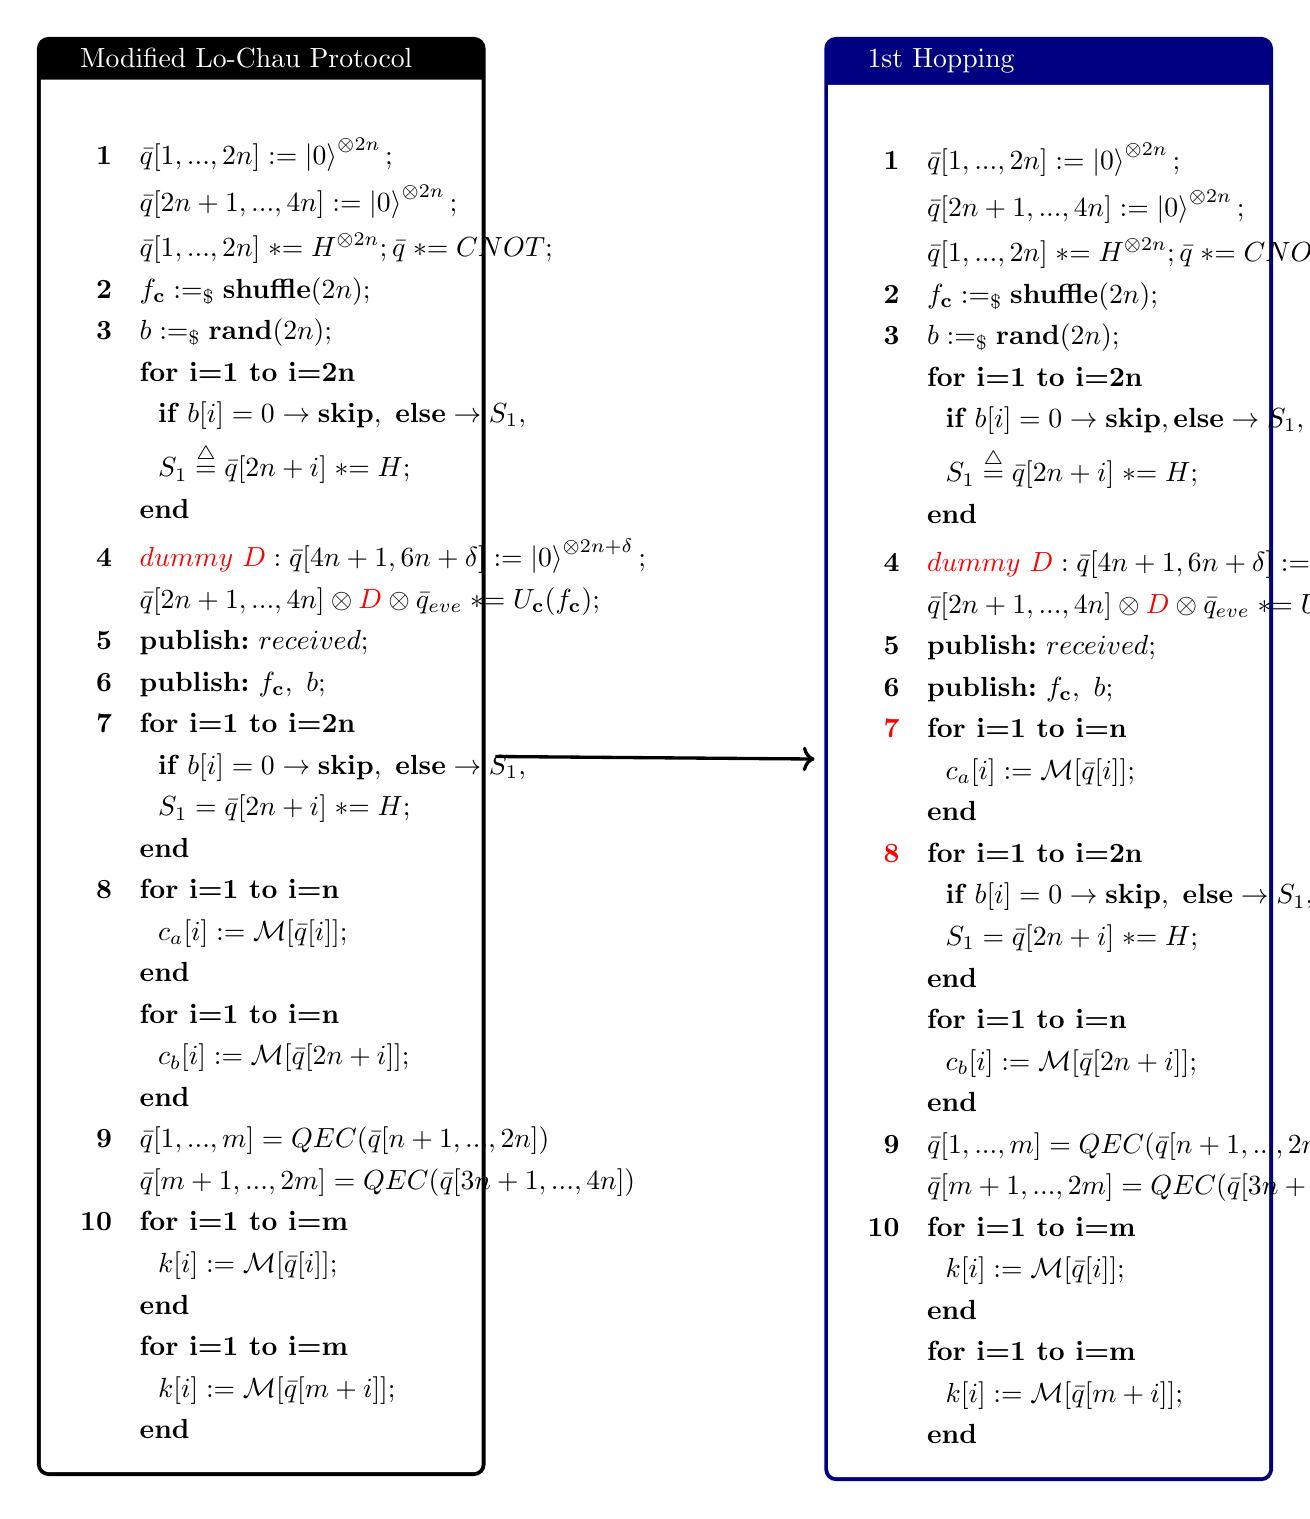
\begin{tikzpicture}[remember picture]
% Left box
\node[anchor=north west] (leftbox) at (0,0) {
\begin{minipage}[t]{0.47\textwidth}
\begin{tcolorbox}[colframe=black!75!black, colback=white, title=Modified Lo-Chau Protocol, width=\textwidth]
\begin{align*}
    \textbf{1} \quad & \bar{q}[1,...,2n] := \ket{0}^{\otimes 2n}; \\
    &\bar{q}[2n+1,...,4n] := \ket{0}^{\otimes 2n};\\
    \quad &\bar{q}[1,...,2n] \asteq H^{\otimes 2n}; \bar{q} \asteq CNOT; \\
    \textbf{2} \quad & f_{\textbf{c}}:=_\$\textbf{shuffle}(2n); \\
    \textbf{3} \quad & b :=_\$ \textbf{rand}(2n); \\
    &\textbf{for i=1 to i=2n}\\
    &~~ \textbf{if }  b[i] = 0 \rightarrow \textbf{skip},~\textbf{else}\rightarrow S_{1},\\
    &~~ S_{1}\stackrel{\triangle}{=}\bar{q}[2n+i] \asteq H ;\\
    &\textbf{end}\\
    \textbf{4} \quad & \textcolor{red}{dummy~D}: \bar{q}[4n+1,6n+\delta]:=\ket{0}^{\otimes 2n+\delta};\\
    &\bar{q}[2n+1,...,4n]\otimes \textcolor{red}{D} \otimes \bar{q}_{eve} \asteq U_{\textbf{c}}(f_{\textbf{c}}); \\
    \textbf{5} \quad & \textbf{publish:}~ received;\\
    \textbf{6} \quad & \textbf{publish:}~ f_{\textbf{c}},~b;\\
    \textbf{7} \quad & \textbf{for i=1 to i=2n}\\
    &~~ \textbf{if }  b[i] = 0 \rightarrow \textbf{skip},~\textbf{else}\rightarrow S_{1} ,\\
    &~~ S_{1}=\bar{q}[2n+i] \asteq H ;\\
    &\textbf{end}\\
    \textbf{8} \quad & \textbf{for~i=1~to~i=n}\\
    &~~ c_a[i]:= \mathcal{M} [\bar{q}[i]];\\
    &\textbf{end}\\
    \quad & \textbf{for~i=1~to~i=n}\\
    &~~ c_b[i]:= \mathcal{M} [\bar{q}[2n+i]];\\
    &\textbf{end}\\
    \textbf{9} \quad & \bar{q}[1,...,m]=QEC(\bar{q}[n+1,...,2n])\\
    \quad & \bar{q}[m+1,...,2m]=QEC(\bar{q}[3n+1,...,4n])\\
    \textbf{10} \quad & \textbf{for~i=1~to~i=m}\\
    &~~ k[i]:= \mathcal{M} [\bar{q}[i]];\\
    &\textbf{end}\\
    & \textbf{for~i=1~to~i=m}\\
    &~~ k[i]:= \mathcal{M} [\bar{q}[m+i]];\\
    &\textbf{end}
\end{align*}
\end{tcolorbox}
\end{minipage}
};

% Right box
\node[anchor=north west] (rightbox) at (10,0) {
\begin{minipage}[t]{0.47\textwidth}
\begin{tcolorbox}[colframe=blue!50!black, colback=white, title=1st Hopping, width=\textwidth]
\begin{align*}
    \textbf{1} \quad & \bar{q}[1,...,2n] := \ket{0}^{\otimes 2n}; \\
    &\bar{q}[2n+1,...,4n] := \ket{0}^{\otimes 2n};\\
    \quad &\bar{q}[1,...,2n] \asteq H^{\otimes 2n}; \bar{q} \asteq CNOT; \\
    \textbf{2} \quad & f_{\textbf{c}}:=_\$\textbf{shuffle}(2n); \\
    \textbf{3} \quad & b :=_\$ \textbf{rand}(2n); \\
    &\textbf{for i=1 to i=2n}\\
    &~~ \textbf{if }  b[i] = 0 \rightarrow \textbf{skip}, \textbf{else}\rightarrow S_{1} ,\\
    &~~ S_{1}\stackrel{\triangle}{=}\bar{q}[2n+i] \asteq H ;\\
    &\textbf{end}\\
    \textbf{4} \quad & \textcolor{red}{dummy~D}: \bar{q}[4n+1,6n+\delta]:=\ket{0}^{\otimes 2n+\delta};\\     &\bar{q}[2n+1,...,4n]\otimes \textcolor{red}{D} \otimes \bar{q}_{eve} \asteq U_{\textbf{c}}(f_{\textbf{c}}); \\
    \textbf{5} \quad & \textbf{publish:}~ received;\\
    \textbf{6} \quad & \textbf{publish:}~ f_{\textbf{c}},~b;\\
    \textbf{\textcolor{red}{7}} \quad & \textbf{for~i=1~to~i=n}\\
    &~~ c_a[i]:= \mathcal{M} [\bar{q}[i]];\\
    &\textbf{end}\\
    \textbf{\textcolor{red}{8}} \quad & \textbf{for i=1 to i=2n}\\
    &~~ \textbf{if }  b[i] = 0 \rightarrow\textbf{skip},~\textbf{else}\rightarrow S_{1} ,\\
    &~~ S_{1}=\bar{q}[2n+i] \asteq H ;\\
    &\textbf{end}\\
    \quad & \textbf{for~i=1~to~i=n}\\
    &~~ c_b[i]:= \mathcal{M} [\bar{q}[2n+i]];\\
    &\textbf{end}\\
    \textbf{9} \quad & \bar{q}[1,...,m]=QEC(\bar{q}[n+1,...,2n])\\
    \quad & \bar{q}[m+1,...,2m]=QEC(\bar{q}[3n+1,...,4n])\\
    \textbf{10} \quad & \textbf{for~i=1~to~i=m}\\
    &~~ k[i]:= \mathcal{M} [\bar{q}[i]];\\
    &\textbf{end}\\
    & \textbf{for~i=1~to~i=m}\\
    &~~ k[i]:= \mathcal{M} [\bar{q}[m+i]];\\
    &\textbf{end}
\end{align*}
\end{tcolorbox}
\end{minipage}
};

% Draw arrow between boxes
\draw[->, very thick] (leftbox.east) -- node[above]{} (rightbox.west);

\end{tikzpicture}
\newpage
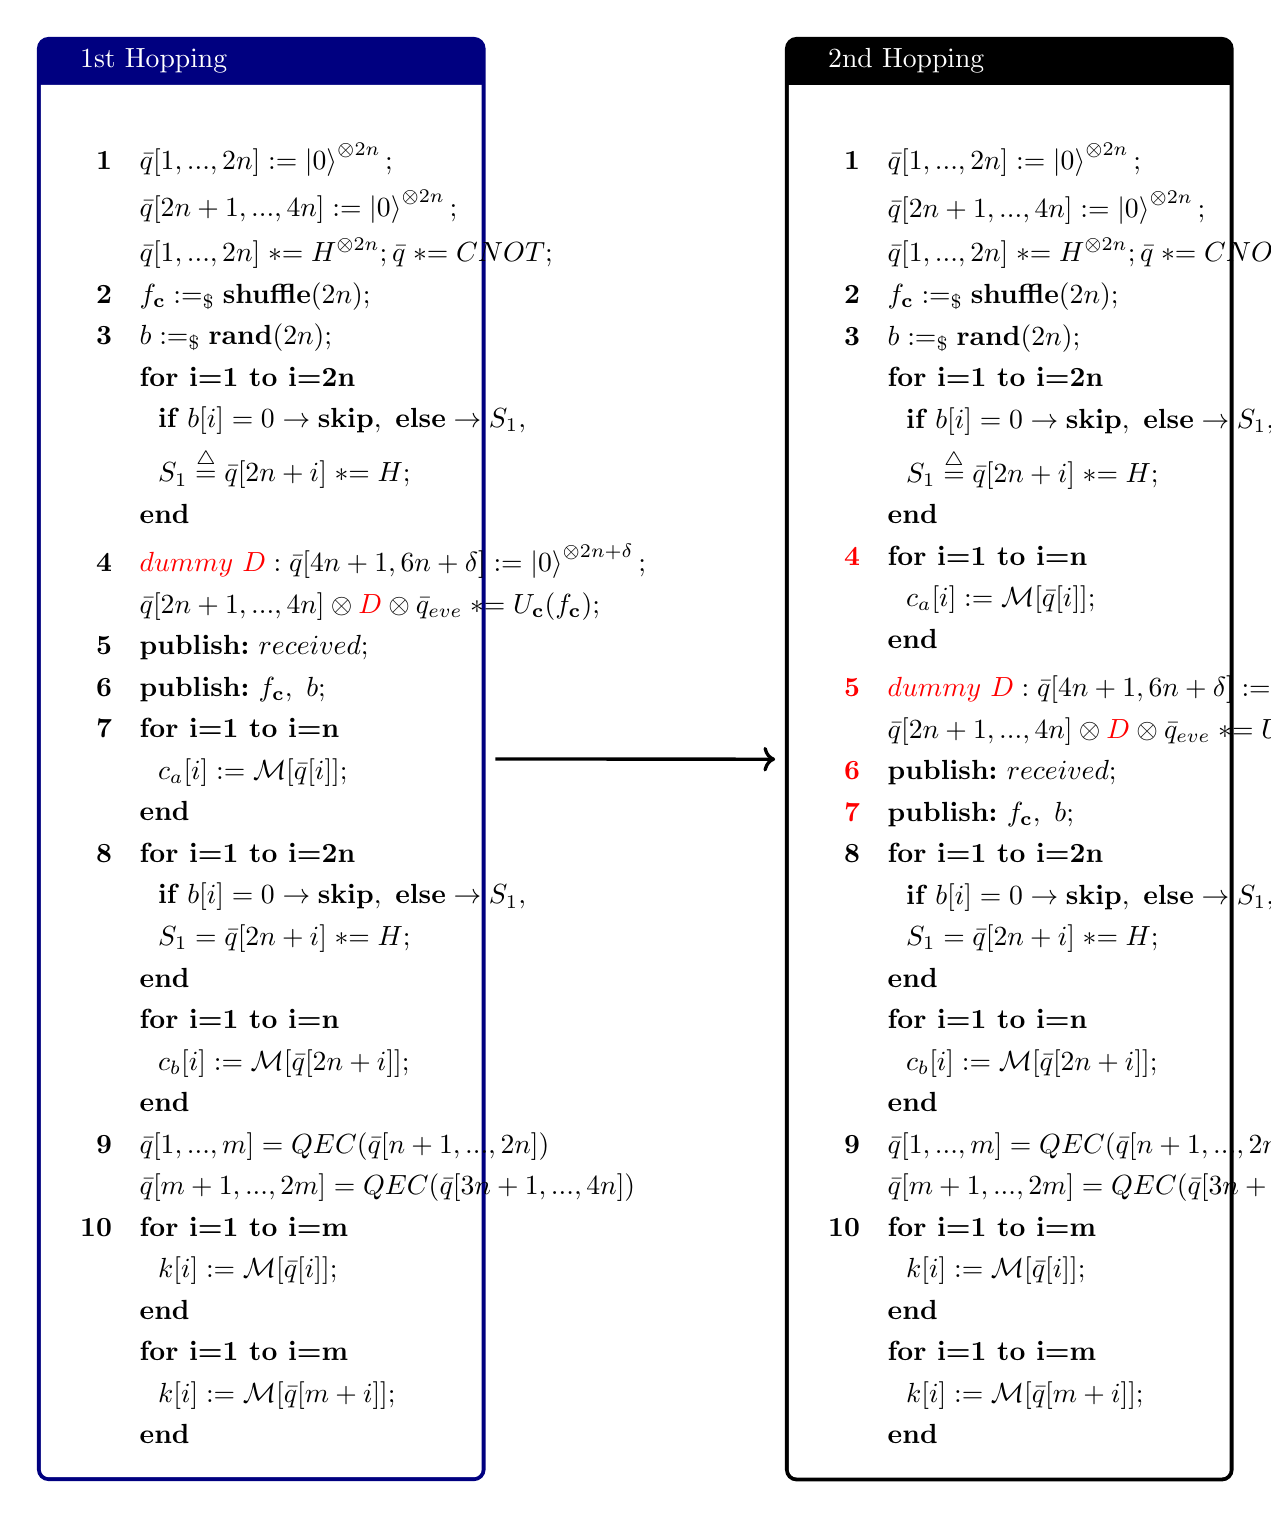
\begin{tikzpicture}[remember picture]

% Left box
\node[anchor=north west] (leftbox) at (0,0) {
\begin{minipage}[t]{0.47\textwidth}
\begin{tcolorbox}[colframe=blue!50!black, colback=white, title=1st Hopping, width=\textwidth]
\begin{align*}
    \textbf{1} \quad & \bar{q}[1,...,2n] := \ket{0}^{\otimes 2n}; \\
    &\bar{q}[2n+1,...,4n] := \ket{0}^{\otimes 2n};\\
    \quad &\bar{q}[1,...,2n] \asteq H^{\otimes 2n}; \bar{q} \asteq CNOT; \\
    \textbf{2} \quad & f_{\textbf{c}}:=_\$\textbf{shuffle}(2n); \\
    \textbf{3} \quad & b :=_\$ \textbf{rand}(2n); \\
    &\textbf{for i=1 to i=2n}\\
    &~~ \textbf{if }  b[i] = 0 \rightarrow \textbf{skip},~\textbf{else}\rightarrow S_{1} ,\\
    &~~ S_{1}\stackrel{\triangle}{=}\bar{q}[2n+i] \asteq H ;\\
    &\textbf{end}\\
    \textbf{4} \quad & \textcolor{red}{dummy~D}: \bar{q}[4n+1,6n+\delta]:=\ket{0}^{\otimes 2n+\delta};\\     &\bar{q}[2n+1,...,4n]\otimes \textcolor{red}{D} \otimes \bar{q}_{eve} \asteq U_{\textbf{c}}(f_{\textbf{c}}); \\
    \textbf{5} \quad & \textbf{publish:}~ received;\\
    \textbf{6} \quad & \textbf{publish:}~ f_{\textbf{c}},~b;\\
    \textbf{{7}} \quad & \textbf{for~i=1~to~i=n}\\
    &~~ c_a[i]:= \mathcal{M} [\bar{q}[i]];\\
    &\textbf{end}\\
    \textbf{{8}} \quad & \textbf{for i=1 to i=2n}\\
    &~~ \textbf{if }  b[i] = 0 \rightarrow \textbf{skip},~\textbf{else}\rightarrow S_{1} ,\\
    &~~ S_{1}=\bar{q}[2n+i] \asteq H ;\\
    &\textbf{end}\\
    \quad & \textbf{for~i=1~to~i=n}\\
    &~~ c_b[i]:= \mathcal{M} [\bar{q}[2n+i]];\\
    &\textbf{end}\\
    \textbf{9} \quad & \bar{q}[1,...,m]=QEC(\bar{q}[n+1,...,2n])\\
    \quad & \bar{q}[m+1,...,2m]=QEC(\bar{q}[3n+1,...,4n])\\
    \textbf{10} \quad & \textbf{for~i=1~to~i=m}\\
    &~~ k[i]:= \mathcal{M} [\bar{q}[i]];\\
    &\textbf{end}
    \\
    & \textbf{for~i=1~to~i=m}\\
    &~~ k[i]:= \mathcal{M} [\bar{q}[m+i]];\\
    &\textbf{end}
\end{align*}
\end{tcolorbox}
\end{minipage}
};

% Right box
\node[anchor=north west] (rightbox) at (9.5,0) {
\begin{minipage}[t]{0.47\textwidth}
\begin{tcolorbox}[colframe=black!50!black, colback=white, title=2nd Hopping, width=\textwidth]
\begin{align*}
    \textbf{1} \quad & \bar{q}[1,...,2n] := \ket{0}^{\otimes 2n}; \\
    &\bar{q}[2n+1,...,4n] := \ket{0}^{\otimes 2n};\\
    \quad &\bar{q}[1,...,2n] \asteq H^{\otimes 2n}; \bar{q} \asteq CNOT; \\
    \textbf{2} \quad & f_{\textbf{c}}:=_\$\textbf{shuffle}(2n); \\
    \textbf{3} \quad & b :=_\$ \textbf{rand}(2n); \\
    &\textbf{for i=1 to i=2n}\\
    &~~ \textbf{if }  b[i] = 0 \rightarrow \textbf{skip},~\textbf{else}\rightarrow S_{1} ,\\
    &~~ S_{1}\stackrel{\triangle}{=}\bar{q}[2n+i] \asteq H ;\\
    &\textbf{end}\\
    \textbf{\textcolor{red}{4}} \quad & \textbf{for~i=1~to~i=n}\\
    &~~ c_a[i]:= \mathcal{M} [\bar{q}[i]];\\
    &\textbf{end}\\
    \textbf{\textcolor{red}{5}} \quad & \textcolor{red}{dummy~D}: \bar{q}[4n+1,6n+\delta]:=\ket{0}^{\otimes 2n+\delta};\\     &\bar{q}[2n+1,...,4n]\otimes \textcolor{red}{D} \otimes \bar{q}_{eve} \asteq U_{\textbf{c}}(f_{\textbf{c}}); \\
    \textbf{\textcolor{red}{6}} \quad & \textbf{publish:}~ received;\\
    \textbf{\textcolor{red}{7}} \quad & \textbf{publish:}~ f_{\textbf{c}},~b;\\
    \textbf{{8}} \quad & \textbf{for i=1 to i=2n}\\
    &~~ \textbf{if }  b[i] = 0 \rightarrow\textbf{skip},~\textbf{else}\rightarrow S_{1} ,\\
    &~~ S_{1}=\bar{q}[2n+i] \asteq H ;\\
    &\textbf{end}\\
    \quad & \textbf{for~i=1~to~i=n}\\
    &~~ c_b[i]:= \mathcal{M} [\bar{q}[2n+i]];\\
    &\textbf{end}\\
    \textbf{9} \quad & \bar{q}[1,...,m]=QEC(\bar{q}[n+1,...,2n])\\
    \quad & \bar{q}[m+1,...,2m]=QEC(\bar{q}[3n+1,...,4n])\\
    \textbf{10} \quad & \textbf{for~i=1~to~i=m}\\
    &~~ k[i]:= \mathcal{M} [\bar{q}[i]];\\
    &\textbf{end}
    \\
    & \textbf{for~i=1~to~i=m}\\
    &~~ k[i]:= \mathcal{M} [\bar{q}[m+i]];\\
    &\textbf{end}
\end{align*}
\end{tcolorbox}
\end{minipage}
};

% Draw arrow between boxes
\draw[->, very thick] (leftbox.east) -- node[above]{} (rightbox.west);

\end{tikzpicture}
\newpage

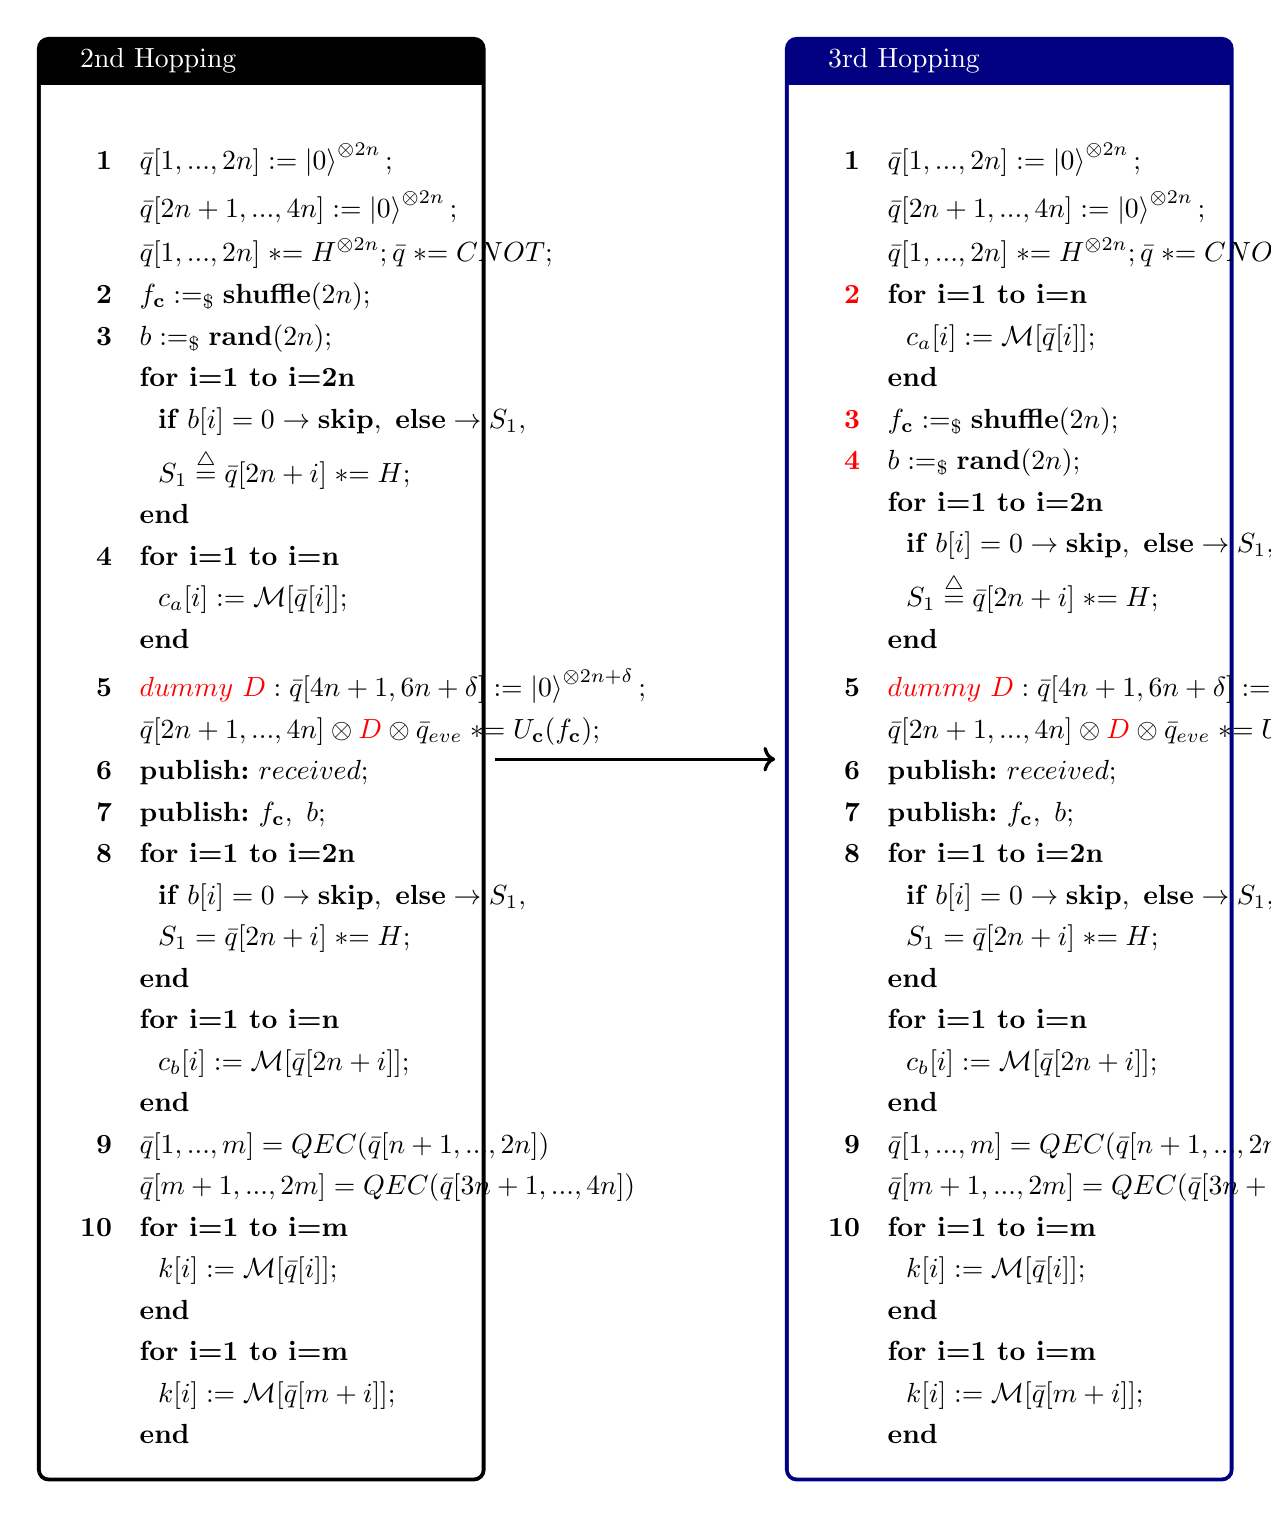
\begin{tikzpicture}[remember picture]

% Left box
\node[anchor=north west] (leftbox) at (0,0) {
\begin{minipage}[t]{0.47\textwidth}
\begin{tcolorbox}[colframe=black!75!black, colback=white, title=2nd Hopping, width=\textwidth]
\begin{align*}
    \textbf{1} \quad & \bar{q}[1,...,2n] := \ket{0}^{\otimes 2n}; \\
    &\bar{q}[2n+1,...,4n] := \ket{0}^{\otimes 2n};\\
    \quad &\bar{q}[1,...,2n] \asteq H^{\otimes 2n}; \bar{q} \asteq CNOT; \\
    \textbf{2} \quad & f_{\textbf{c}}:=_\$\textbf{shuffle}(2n); \\
    \textbf{3} \quad & b :=_\$ \textbf{rand}(2n); \\
    &\textbf{for i=1 to i=2n}\\
    &~~ \textbf{if }  b[i] = 0 \rightarrow \textbf{skip},~\textbf{else}\rightarrow S_{1} ,\\
    &~~ S_{1}\stackrel{\triangle}{=}\bar{q}[2n+i] \asteq H ;\\
    &\textbf{end}\\
    \textbf{{4}} \quad & \textbf{for~i=1~to~i=n}\\
    &~~ c_a[i]:= \mathcal{M} [\bar{q}[i]];\\
    &\textbf{end}\\
    \textbf{{5}} \quad & \textcolor{red}{dummy~D}: \bar{q}[4n+1,6n+\delta]:=\ket{0}^{\otimes 2n+\delta};\\     &\bar{q}[2n+1,...,4n]\otimes \textcolor{red}{D} \otimes \bar{q}_{eve} \asteq U_{\textbf{c}}(f_{\textbf{c}}); \\
    \textbf{{6}} \quad & \textbf{publish:}~ received;\\
    \textbf{{7}} \quad & \textbf{publish:}~ f_{\textbf{c}},~b;\\
    \textbf{{8}} \quad & \textbf{for i=1 to i=2n}\\
    &~~ \textbf{if }  b[i] = 0 \rightarrow \textbf{skip},~\textbf{else}\rightarrow S_{1} ,\\
    &~~ S_{1}=\bar{q}[2n+i] \asteq H ;\\
    &\textbf{end}\\
    \quad & \textbf{for~i=1~to~i=n}\\
    &~~ c_b[i]:= \mathcal{M} [\bar{q}[2n+i]];\\
    &\textbf{end}\\
    \textbf{9} \quad & \bar{q}[1,...,m]=QEC(\bar{q}[n+1,...,2n])\\
    \quad & \bar{q}[m+1,...,2m]=QEC(\bar{q}[3n+1,...,4n])\\
    \textbf{10} \quad & \textbf{for~i=1~to~i=m}\\
    &~~ k[i]:= \mathcal{M} [\bar{q}[i]];\\
    &\textbf{end}
    \\
    & \textbf{for~i=1~to~i=m}\\
    &~~ k[i]:= \mathcal{M} [\bar{q}[m+i]];\\
    &\textbf{end}
\end{align*}
\end{tcolorbox}
\end{minipage}
};

% Right box
\node[anchor=north west] (rightbox) at (9.5,0) {
\begin{minipage}[t]{0.47\textwidth}
\begin{tcolorbox}[colframe=blue!50!black, colback=white, title=3rd Hopping, width=\textwidth]
\begin{align*}
    \textbf{1} \quad & \bar{q}[1,...,2n] := \ket{0}^{\otimes 2n}; \\
    &\bar{q}[2n+1,...,4n] := \ket{0}^{\otimes 2n};\\
    \quad &\bar{q}[1,...,2n] \asteq H^{\otimes 2n}; \bar{q} \asteq CNOT; \\
    \textbf{\textcolor{red}{2}} \quad & \textbf{for~i=1~to~i=n}\\
    &~~ c_a[i]:= \mathcal{M} [\bar{q}[i]];\\
    &\textbf{end}\\
    \textbf{\textcolor{red}{3}} \quad & f_{\textbf{c}}:=_\$\textbf{shuffle}(2n); \\
    \textbf{\textcolor{red}{4}} \quad & b :=_\$ \textbf{rand}(2n); \\
    &\textbf{for i=1 to i=2n}\\
    &~~ \textbf{if }  b[i] = 0 \rightarrow \textbf{skip},~\textbf{else}\rightarrow S_{1} ,\\
    &~~ S_{1}\stackrel{\triangle}{=}\bar{q}[2n+i] \asteq H ;\\
    &\textbf{end}\\
    \textbf{{5}} \quad & \textcolor{red}{dummy~D}: \bar{q}[4n+1,6n+\delta]:=\ket{0}^{\otimes 2n+\delta};\\     &\bar{q}[2n+1,...,4n]\otimes \textcolor{red}{D} \otimes \bar{q}_{eve} \asteq U_{\textbf{c}}(f_{\textbf{c}}); \\
    \textbf{{6}} \quad & \textbf{publish:}~ received;\\
    \textbf{{7}} \quad & \textbf{publish:}~ f_{\textbf{c}},~b;\\
    \textbf{{8}} \quad & \textbf{for i=1 to i=2n}\\
    &~~ \textbf{if }  b[i] = 0 \rightarrow \textbf{skip},~\textbf{else}\rightarrow S_{1} ,\\
    &~~ S_{1}=\bar{q}[2n+i] \asteq H ;\\
    &\textbf{end}\\
    \quad & \textbf{for~i=1~to~i=n}\\
    &~~ c_b[i]:= \mathcal{M} [\bar{q}[2n+i]];\\
    &\textbf{end}\\
    \textbf{9} \quad & \bar{q}[1,...,m]=QEC(\bar{q}[n+1,...,2n])\\
    \quad & \bar{q}[m+1,...,2m]=QEC(\bar{q}[3n+1,...,4n])\\
    \textbf{10} \quad & \textbf{for~i=1~to~i=m}\\
    &~~ k[i]:= \mathcal{M} [\bar{q}[i]];\\
    &\textbf{end}
    \\
    & \textbf{for~i=1~to~i=m}\\
    &~~ k[i]:= \mathcal{M} [\bar{q}[m+i]];\\
    &\textbf{end}
\end{align*}
\end{tcolorbox}
\end{minipage}
};

% Draw arrow between boxes
\draw[->, very thick] (leftbox.east) -- node[above]{} (rightbox.west);

\end{tikzpicture}
\newpage

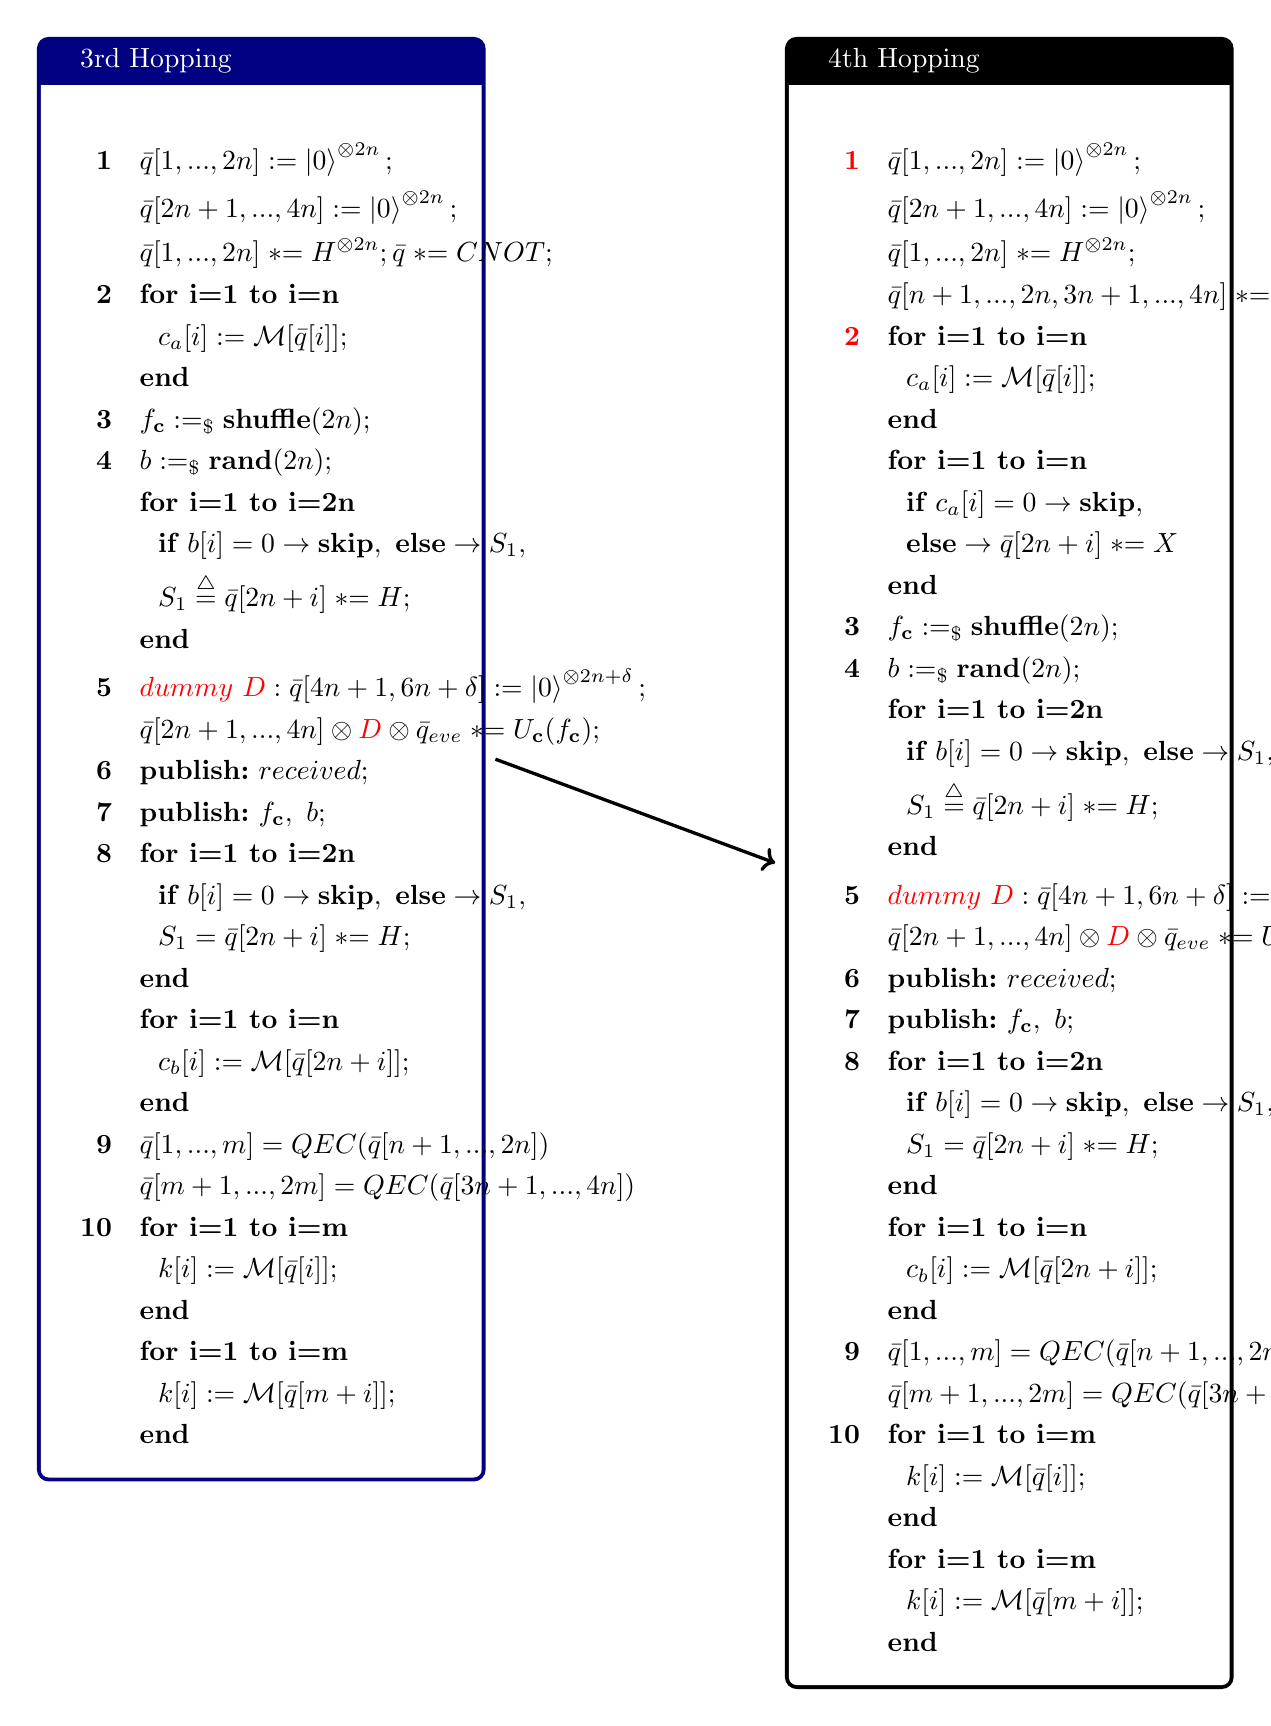
\begin{tikzpicture}[remember picture]

% Left box
\node[anchor=north west] (leftbox) at (0,0) {
\begin{minipage}[t]{0.47\textwidth}
\begin{tcolorbox}[colframe=blue!50!black, colback=white, title=3rd Hopping, width=\textwidth]
\begin{align*}
    \textbf{1} \quad & \bar{q}[1,...,2n] := \ket{0}^{\otimes 2n}; \\
    &\bar{q}[2n+1,...,4n] := \ket{0}^{\otimes 2n};\\
    \quad &\bar{q}[1,...,2n] \asteq H^{\otimes 2n}; \bar{q} \asteq CNOT; \\
    \textbf{{2}} \quad & \textbf{for~i=1~to~i=n}\\
    &~~ c_a[i]:= \mathcal{M} [\bar{q}[i]];\\
    &\textbf{end}\\
    \textbf{{3}} \quad & f_{\textbf{c}}:=_\$\textbf{shuffle}(2n); \\
    \textbf{{4}} \quad & b :=_\$ \textbf{rand}(2n); \\
    &\textbf{for i=1 to i=2n}\\
    &~~ \textbf{if }  b[i] = 0 \rightarrow \textbf{skip},~\textbf{else}\rightarrow S_{1} ,\\
    &~~ S_{1}\stackrel{\triangle}{=}\bar{q}[2n+i] \asteq H ;\\
    &\textbf{end}\\
    \textbf{{5}} \quad & \textcolor{red}{dummy~D}: \bar{q}[4n+1,6n+\delta]:=\ket{0}^{\otimes 2n+\delta};\\     &\bar{q}[2n+1,...,4n]\otimes \textcolor{red}{D} \otimes \bar{q}_{eve} \asteq U_{\textbf{c}}(f_{\textbf{c}}); \\
    \textbf{{6}} \quad & \textbf{publish:}~ received;\\
    \textbf{{7}} \quad & \textbf{publish:}~ f_{\textbf{c}},~b;\\
    \textbf{{8}} \quad & \textbf{for i=1 to i=2n}\\
    &~~ \textbf{if }  b[i] = 0 \rightarrow \textbf{skip},~\textbf{else}\rightarrow S_{1} ,\\
    &~~ S_{1}=\bar{q}[2n+i] \asteq H ;\\
    &\textbf{end}\\
    \quad & \textbf{for~i=1~to~i=n}\\
    &~~ c_b[i]:= \mathcal{M} [\bar{q}[2n+i]];\\
    &\textbf{end}\\
    \textbf{9} \quad & \bar{q}[1,...,m]=QEC(\bar{q}[n+1,...,2n])\\
    \quad & \bar{q}[m+1,...,2m]=QEC(\bar{q}[3n+1,...,4n])\\
    \textbf{10} \quad & \textbf{for~i=1~to~i=m}\\
    &~~ k[i]:= \mathcal{M} [\bar{q}[i]];\\
    &\textbf{end}
    \\
    & \textbf{for~i=1~to~i=m}\\
    &~~ k[i]:= \mathcal{M} [\bar{q}[m+i]];\\
    &\textbf{end}
\end{align*}
\end{tcolorbox}
\end{minipage}
};

% Right box
\node[anchor=north west] (rightbox) at (9.5,0) {
\begin{minipage}[t]{0.47\textwidth}
\begin{tcolorbox}[colframe=black!50!black, colback=white, title=4th Hopping, width=\textwidth]
\begin{align*}
    \textbf{\textcolor{red}{1}} \quad & \bar{q}[1,...,2n] := \ket{0}^{\otimes 2n}; \\
    &\bar{q}[2n+1,...,4n] := \ket{0}^{\otimes 2n};\\
    \quad &\bar{q}[1,...,2n] \asteq H^{\otimes 2n}; \\
    &\bar{q}[n+1,...,2n,3n+1,...,4n] \asteq CNOT; \\
    \textbf{\textcolor{red}{2}} \quad & \textbf{for~i=1~to~i=n}\\
    &~~ c_a[i]:= \mathcal{M} [\bar{q}[i]];\\
    &\textbf{end}\\
    &\textbf{for i=1 to i=n}\\
    &~~ \textbf{if }  c_a[i]=0\rightarrow \textbf{skip},\\ &~~\textbf{else}   \rightarrow \bar{q}[2n+i]\asteq X\\
    &\textbf{end}\ \\
    \textbf{{3}} \quad & f_{\textbf{c}}:=_\$\textbf{shuffle}(2n); \\
    \textbf{{4}} \quad & b :=_\$ \textbf{rand}(2n); \\
    &\textbf{for i=1 to i=2n}\\
    &~~ \textbf{if }  b[i] = 0 \rightarrow \textbf{skip},~\textbf{else}\rightarrow S_{1} ,\\
    &~~ S_{1}\stackrel{\triangle}{=}\bar{q}[2n+i] \asteq H ;\\
    &\textbf{end}\\
    \textbf{{5}} \quad & \textcolor{red}{dummy~D}: \bar{q}[4n+1,6n+\delta]:=\ket{0}^{\otimes 2n+\delta};\\     &\bar{q}[2n+1,...,4n]\otimes \textcolor{red}{D} \otimes \bar{q}_{eve} \asteq U_{\textbf{c}}(f_{\textbf{c}}); \\
    \textbf{{6}} \quad & \textbf{publish:}~ received;\\
    \textbf{{7}} \quad & \textbf{publish:}~ f_{\textbf{c}},~b;\\
    \textbf{{8}} \quad & \textbf{for i=1 to i=2n}\\
    &~~ \textbf{if }  b[i] = 0 \rightarrow \textbf{skip},~\textbf{else}\rightarrow S_{1} ,\\
    &~~ S_{1}=\bar{q}[2n+i] \asteq H ;\\
    &\textbf{end}\\
    \quad & \textbf{for~i=1~to~i=n}\\
    &~~ c_b[i]:= \mathcal{M} [\bar{q}[2n+i]];\\
    &\textbf{end}\\
    \textbf{9} \quad & \bar{q}[1,...,m]=QEC(\bar{q}[n+1,...,2n])\\
    \quad & \bar{q}[m+1,...,2m]=QEC(\bar{q}[3n+1,...,4n])\\
    \textbf{10} \quad & \textbf{for~i=1~to~i=m}\\
    &~~ k[i]:= \mathcal{M} [\bar{q}[i]];\\
    &\textbf{end}
    \\
    & \textbf{for~i=1~to~i=m}\\
    &~~ k[i]:= \mathcal{M} [\bar{q}[m+i]];\\
    &\textbf{end}
\end{align*}
\end{tcolorbox}
\end{minipage}
};

% Draw arrow between boxes
\draw[->, very thick] (leftbox.east) -- node[above]{} (rightbox.west);

\end{tikzpicture}
\newpage

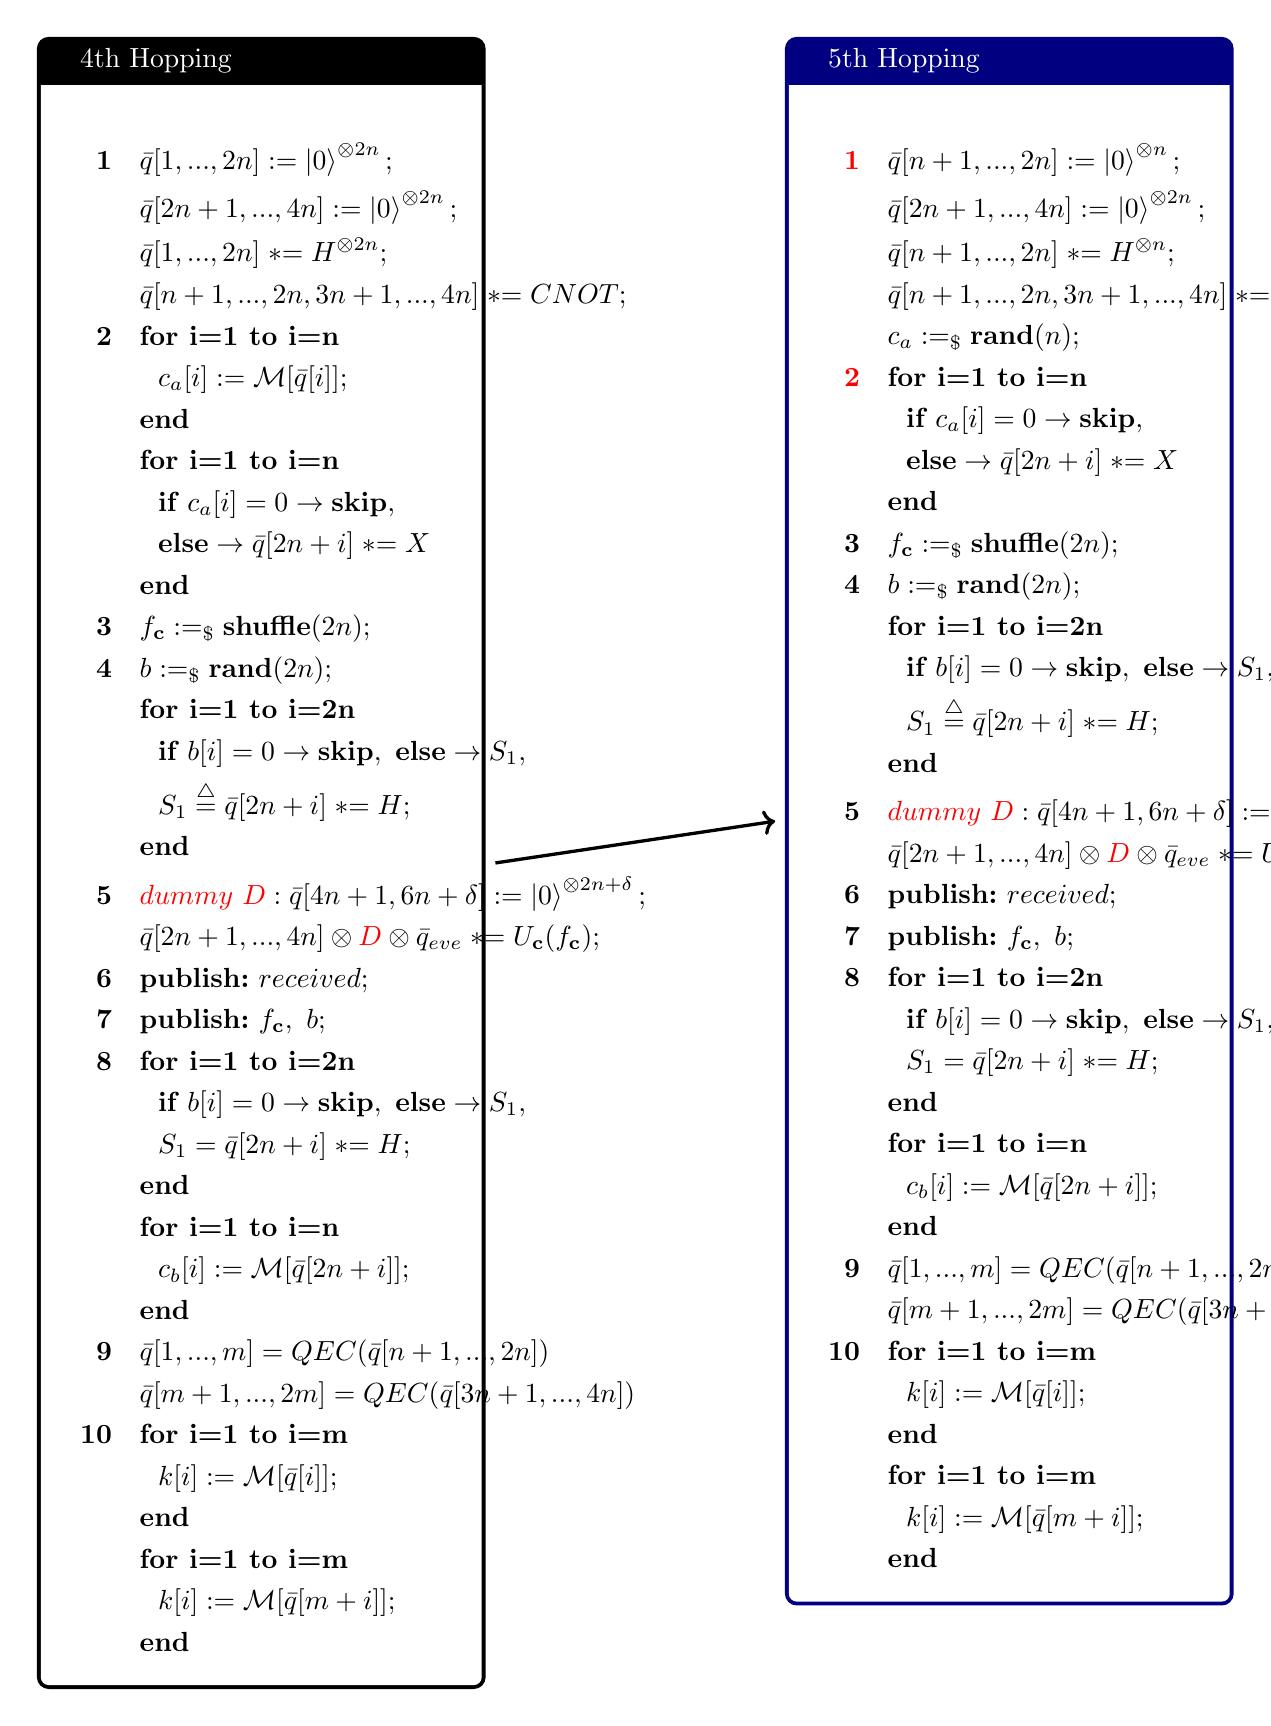
\begin{tikzpicture}[remember picture]

% Left box
\node[anchor=north west] (leftbox) at (0,0) {
\begin{minipage}[t]{0.47\textwidth}
\begin{tcolorbox}[colframe=black!75!black, colback=white, title=4th Hopping, width=\textwidth]
\begin{align*}
    \textbf{{1}} \quad & \bar{q}[1,...,2n] := \ket{0}^{\otimes 2n}; \\
    &\bar{q}[2n+1,...,4n] := \ket{0}^{\otimes 2n};\\
    \quad &\bar{q}[1,...,2n] \asteq H^{\otimes 2n}; \\
    &\bar{q}[n+1,...,2n,3n+1,...,4n] \asteq CNOT; \\
    \textbf{{2}} \quad &  \textbf{for~i=1~to~i=n}\\
    &~~ c_a[i]:= \mathcal{M} [\bar{q}[i]];\\
    &\textbf{end}\\
    &\textbf{for i=1 to i=n}\\
    &~~ \textbf{if }  c_a[i]=0\rightarrow \textbf{skip},\\ &~~\textbf{else}   \rightarrow \bar{q}[2n+i]\asteq X\\
    &\textbf{end}\ \\
    \textbf{{3}} \quad & f_{\textbf{c}}:=_\$\textbf{shuffle}(2n); \\
    \textbf{{4}} \quad & b :=_\$ \textbf{rand}(2n); \\
    &\textbf{for i=1 to i=2n}\\
    &~~ \textbf{if }  b[i] = 0 \rightarrow \textbf{skip},~\textbf{else}\rightarrow S_{1} ,\\
    &~~ S_{1}\stackrel{\triangle}{=}\bar{q}[2n+i] \asteq H ;\\
    &\textbf{end}\\
    \textbf{{5}} \quad & \textcolor{red}{dummy~D}: \bar{q}[4n+1,6n+\delta]:=\ket{0}^{\otimes 2n+\delta};\\     &\bar{q}[2n+1,...,4n]\otimes \textcolor{red}{D} \otimes \bar{q}_{eve} \asteq U_{\textbf{c}}(f_{\textbf{c}}); \\
    \textbf{{6}} \quad & \textbf{publish:}~ received;\\
    \textbf{{7}} \quad & \textbf{publish:}~ f_{\textbf{c}},~b;\\
    \textbf{{8}} \quad & \textbf{for i=1 to i=2n}\\
    &~~ \textbf{if }  b[i] = 0 \rightarrow \textbf{skip},~\textbf{else}\rightarrow S_{1} ,\\
    &~~ S_{1}=\bar{q}[2n+i] \asteq H ;\\
    &\textbf{end}\\
    \quad & \textbf{for~i=1~to~i=n}\\
    &~~ c_b[i]:= \mathcal{M} [\bar{q}[2n+i]];\\
    &\textbf{end}\\
    \textbf{9} \quad & \bar{q}[1,...,m]=QEC(\bar{q}[n+1,...,2n])\\
    \quad & \bar{q}[m+1,...,2m]=QEC(\bar{q}[3n+1,...,4n])\\
    \textbf{10} \quad & \textbf{for~i=1~to~i=m}\\
    &~~ k[i]:= \mathcal{M} [\bar{q}[i]];\\
    &\textbf{end}
    \\
    & \textbf{for~i=1~to~i=m}\\
    &~~ k[i]:= \mathcal{M} [\bar{q}[m+i]];\\
    &\textbf{end}
\end{align*}
\end{tcolorbox}
\end{minipage}
};

% Right box
\node[anchor=north west] (rightbox) at (9.5,0) {
\begin{minipage}[t]{0.47\textwidth}
\begin{tcolorbox}[colframe=blue!50!black, colback=white, title=5th Hopping, width=\textwidth]
\begin{align*}
    \textbf{\textcolor{red}{1}} \quad &\bar{q}[n+1,...,2n] := \ket{0}^{\otimes n};\\
    &\bar{q}[2n+1,...,4n] := \ket{0}^{\otimes 2n};\\
    \quad &\bar{q}[n+1,...,2n] \asteq H^{\otimes n}; \\
    &\bar{q}[n+1,...,2n,3n+1,...,4n] \asteq CNOT; \\
    & c_a :=_\$ \textbf{rand}(n); \\ \textbf{\textcolor{red}{2}} \quad &\textbf{for i=1 to i=n}\\
    &~~ \textbf{if }  c_a[i] = 0 \rightarrow \textbf{skip},\\ &~~\textbf{else}   \rightarrow \bar{q}[2n+i]\asteq X\\
    &\textbf{end}\ \\
    \textbf{{3}} \quad & f_{\textbf{c}}:=_\$\textbf{shuffle}(2n); \\
    \textbf{{4}} \quad & b :=_\$ \textbf{rand}(2n); \\
    &\textbf{for i=1 to i=2n}\\
    &~~ \textbf{if }  b[i] = 0 \rightarrow \textbf{skip},~\textbf{else}\rightarrow S_{1} ,\\
    &~~ S_{1}\stackrel{\triangle}{=}\bar{q}[2n+i] \asteq H ;\\
    &\textbf{end}\\
    \textbf{{5}} \quad & \textcolor{red}{dummy~D}: \bar{q}[4n+1,6n+\delta]:=\ket{0}^{\otimes 2n+\delta};\\     &\bar{q}[2n+1,...,4n]\otimes \textcolor{red}{D} \otimes \bar{q}_{eve} \asteq U_{\textbf{c}}(f_{\textbf{c}}); \\
    \textbf{{6}} \quad & \textbf{publish:}~ received;\\
    \textbf{{7}} \quad & \textbf{publish:}~ f_{\textbf{c}},~b;\\
    \textbf{{8}} \quad & \textbf{for i=1 to i=2n}\\
    &~~ \textbf{if }  b[i] = 0 \rightarrow \textbf{skip},~\textbf{else}\rightarrow S_{1} ,\\
    &~~ S_{1}=\bar{q}[2n+i] \asteq H ;\\
    &\textbf{end}\\
    \quad & \textbf{for~i=1~to~i=n}\\
    &~~ c_b[i]:= \mathcal{M} [\bar{q}[2n+i]];\\
    &\textbf{end}\\
    \textbf{9} \quad & \bar{q}[1,...,m]=QEC(\bar{q}[n+1,...,2n])\\
    \quad & \bar{q}[m+1,...,2m]=QEC(\bar{q}[3n+1,...,4n])\\
    \textbf{10} \quad & \textbf{for~i=1~to~i=m}\\
    &~~ k[i]:= \mathcal{M} [\bar{q}[i]];\\
    &\textbf{end}
    \\
    & \textbf{for~i=1~to~i=m}\\
    &~~ k[i]:= \mathcal{M} [\bar{q}[m+i]];\\
    &\textbf{end}
\end{align*}
\end{tcolorbox}
\end{minipage}
};

% Draw arrow between boxes
\draw[->, very thick] (leftbox.east) -- node[above]{} (rightbox.west);

\end{tikzpicture}
\newpage

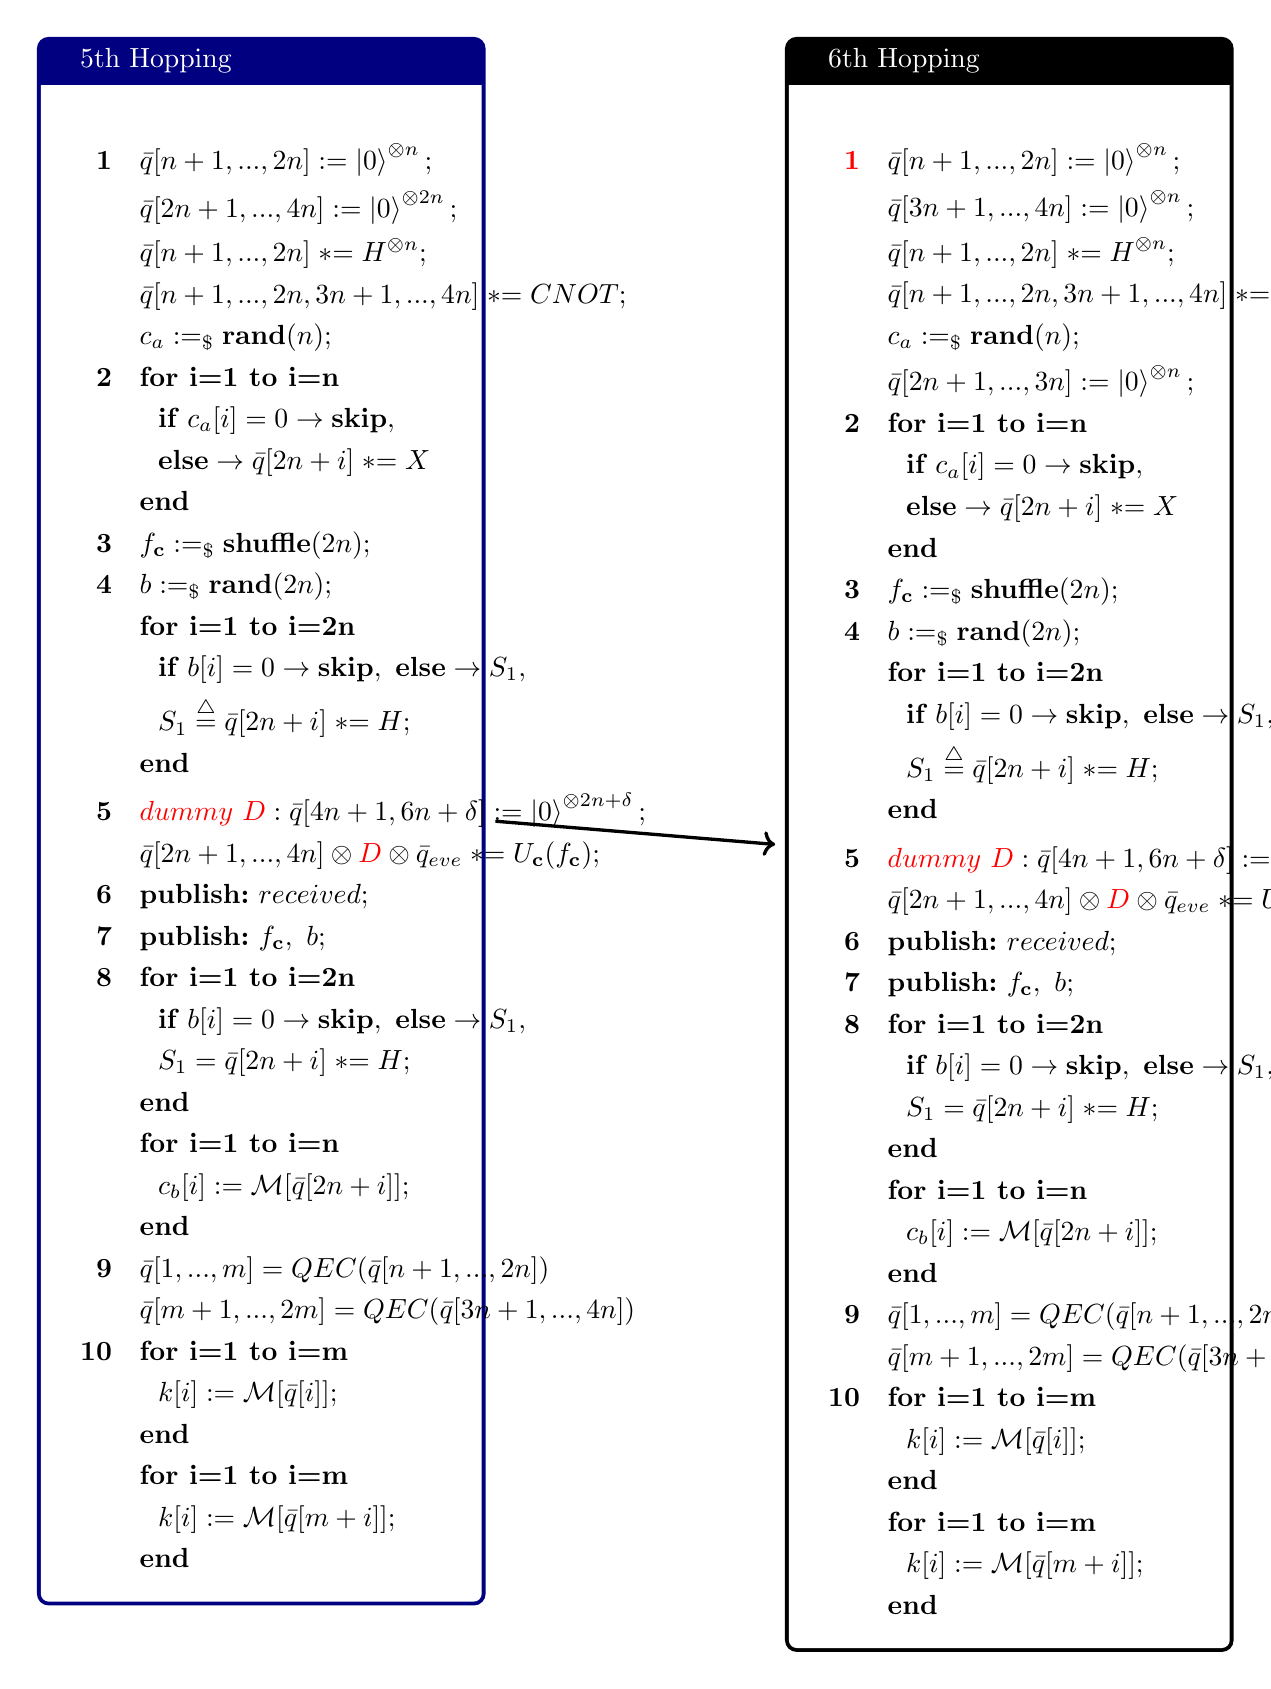
\begin{tikzpicture}[remember picture]

% Left box
\node[anchor=north west] (leftbox) at (0,0) {
\begin{minipage}[t]{0.47\textwidth}
\begin{tcolorbox}[colframe=blue!50!black, colback=white, title=5th Hopping, width=\textwidth]
\begin{align*}
    \textbf{{1}} \quad &\bar{q}[n+1,...,2n] := \ket{0}^{\otimes n};\\
    &\bar{q}[2n+1,...,4n] := \ket{0}^{\otimes 2n};\\
    \quad &\bar{q}[n+1,...,2n] \asteq H^{\otimes n}; \\
    &\bar{q}[n+1,...,2n,3n+1,...,4n] \asteq CNOT; \\
    & c_a :=_\$ \textbf{rand}(n); \\ 
    \textbf{{2}} \quad &\textbf{for i=1 to i=n}\\
    &~~ \textbf{if }  c_a[i] = 0 \rightarrow \textbf{skip},\\ &~~\textbf{else}   \rightarrow \bar{q}[2n+i]\asteq X\\
    &\textbf{end}\ \\
    \textbf{{3}} \quad & f_{\textbf{c}}:=_\$\textbf{shuffle}(2n); \\
    \textbf{{4}} \quad & b :=_\$ \textbf{rand}(2n); \\
    &\textbf{for i=1 to i=2n}\\
    &~~ \textbf{if }  b[i] = 0 \rightarrow \textbf{skip},~\textbf{else}\rightarrow S_{1} ,\\
    &~~ S_{1}\stackrel{\triangle}{=}\bar{q}[2n+i] \asteq H ;\\
    &\textbf{end}\\
    \textbf{{5}} \quad & \textcolor{red}{dummy~D}: \bar{q}[4n+1,6n+\delta]:=\ket{0}^{\otimes 2n+\delta};\\     &\bar{q}[2n+1,...,4n]\otimes \textcolor{red}{D} \otimes \bar{q}_{eve} \asteq U_{\textbf{c}}(f_{\textbf{c}}); \\
    \textbf{{6}} \quad & \textbf{publish:}~ received;\\
    \textbf{{7}} \quad & \textbf{publish:}~ f_{\textbf{c}},~b;\\
    \textbf{{8}} \quad & \textbf{for i=1 to i=2n}\\
    &~~ \textbf{if }  b[i] = 0 \rightarrow \textbf{skip},~\textbf{else}\rightarrow S_{1} ,\\
    &~~ S_{1}=\bar{q}[2n+i] \asteq H ;\\
    &\textbf{end}\\
    \quad & \textbf{for~i=1~to~i=n}\\
    &~~ c_b[i]:= \mathcal{M} [\bar{q}[2n+i]];\\
    &\textbf{end}\\
    \textbf{9} \quad & \bar{q}[1,...,m]=QEC(\bar{q}[n+1,...,2n])\\
    \quad & \bar{q}[m+1,...,2m]=QEC(\bar{q}[3n+1,...,4n])\\
    \textbf{10} \quad & \textbf{for~i=1~to~i=m}\\
    &~~ k[i]:= \mathcal{M} [\bar{q}[i]];\\
    &\textbf{end}
    \\
    & \textbf{for~i=1~to~i=m}\\
    &~~ k[i]:= \mathcal{M} [\bar{q}[m+i]];\\
    &\textbf{end}
\end{align*}
\end{tcolorbox}
\end{minipage}
};

% Right box
\node[anchor=north west] (rightbox) at (9.5,0) {
\begin{minipage}[t]{0.47\textwidth}
\begin{tcolorbox}[colframe=black!50!black, colback=white, title=6th Hopping, width=\textwidth]
\begin{align*}
    \textbf{\textcolor{red}{1}} \quad &\bar{q}[n+1,...,2n] := \ket{0}^{\otimes n};\\
    &\bar{q}[3n+1,...,4n] := \ket{0}^{\otimes n};\\
    \quad &\bar{q}[n+1,...,2n] \asteq H^{\otimes n}; \\
    &\bar{q}[n+1,...,2n,3n+1,...,4n] \asteq CNOT; \\
    & c_a :=_\$ \textbf{rand}(n); \\ 
    &\bar{q}[2n+1,...,3n] := \ket{0}^{\otimes n};\\
    \textbf{{2}} \quad &\textbf{for i=1 to i=n}\\
    &~~ \textbf{if }  c_a[i] = 0 \rightarrow \textbf{skip},\\ &~~\textbf{else}   \rightarrow \bar{q}[2n+i]\asteq X\\
    &\textbf{end}\ \\
    \textbf{{3}} \quad & f_{\textbf{c}}:=_\$\textbf{shuffle}(2n); \\
    \textbf{{4}} \quad & b :=_\$ \textbf{rand}(2n); \\
    &\textbf{for i=1 to i=2n}\\
    &~~ \textbf{if }  b[i] = 0 \rightarrow \textbf{skip},~\textbf{else}\rightarrow S_{1} ,\\
    &~~ S_{1}\stackrel{\triangle}{=}\bar{q}[2n+i] \asteq H ;\\
    &\textbf{end}\\
    \textbf{{5}} \quad & \textcolor{red}{dummy~D}: \bar{q}[4n+1,6n+\delta]:=\ket{0}^{\otimes 2n+\delta};\\     &\bar{q}[2n+1,...,4n]\otimes \textcolor{red}{D} \otimes \bar{q}_{eve} \asteq U_{\textbf{c}}(f_{\textbf{c}}); \\
    \textbf{{6}} \quad & \textbf{publish:}~ received;\\
    \textbf{{7}} \quad & \textbf{publish:}~ f_{\textbf{c}},~b;\\
    \textbf{{8}} \quad & \textbf{for i=1 to i=2n}\\
    &~~ \textbf{if }  b[i] = 0 \rightarrow \textbf{skip},~\textbf{else}\rightarrow S_{1} ,\\
    &~~ S_{1}=\bar{q}[2n+i] \asteq H ;\\
    &\textbf{end}\\
    \quad & \textbf{for~i=1~to~i=n}\\
    &~~ c_b[i]:= \mathcal{M} [\bar{q}[2n+i]];\\
    &\textbf{end}\\
    \textbf{9} \quad & \bar{q}[1,...,m]=QEC(\bar{q}[n+1,...,2n])\\
    \quad & \bar{q}[m+1,...,2m]=QEC(\bar{q}[3n+1,...,4n])\\
    \textbf{10} \quad & \textbf{for~i=1~to~i=m}\\
    &~~ k[i]:= \mathcal{M} [\bar{q}[i]];\\
    &\textbf{end}
    \\
    & \textbf{for~i=1~to~i=m}\\
    &~~ k[i]:= \mathcal{M} [\bar{q}[m+i]];\\
    &\textbf{end}
\end{align*}
\end{tcolorbox}
\end{minipage}
};

% Draw arrow between boxes
\draw[->, very thick] (leftbox.east) -- node[above]{} (rightbox.west);

\end{tikzpicture}
\newpage

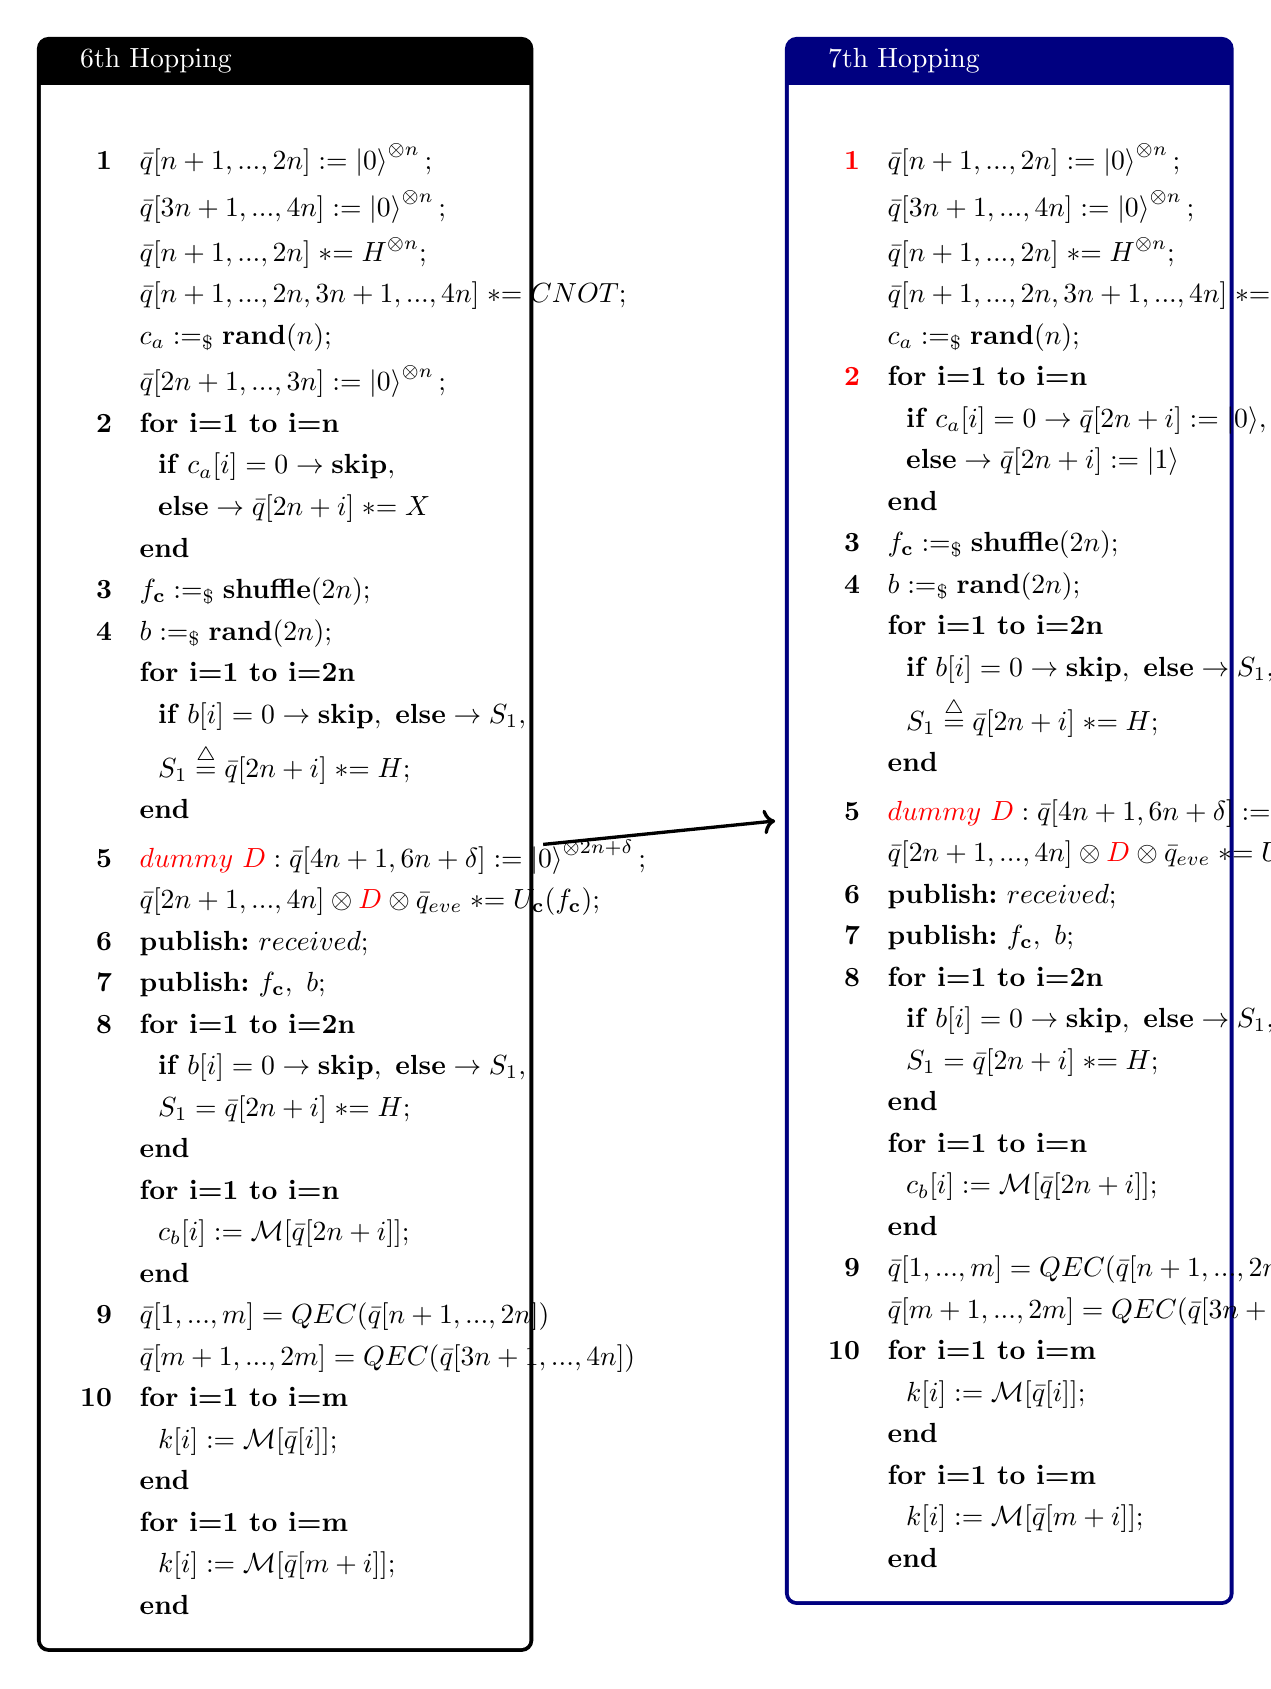
\begin{tikzpicture}[remember picture]

% Left box
\node[anchor=north west] (leftbox) at (0,0) {
\begin{minipage}[t]{0.52\textwidth}
\begin{tcolorbox}[colframe=black!75!black, colback=white, title=6th Hopping, width=\textwidth]
\begin{align*}
    \textbf{{1}} \quad &\bar{q}[n+1,...,2n] := \ket{0}^{\otimes n};\\
    &\bar{q}[3n+1,...,4n] := \ket{0}^{\otimes n};\\
    \quad &\bar{q}[n+1,...,2n] \asteq H^{\otimes n}; \\
    &\bar{q}[n+1,...,2n,3n+1,...,4n] \asteq CNOT; \\
    & c_a :=_\$ \textbf{rand}(n); \\ 
    &\bar{q}[2n+1,...,3n] := \ket{0}^{\otimes n};\\
    \textbf{{2}} \quad &\textbf{for i=1 to i=n}\\
    &~~ \textbf{if }  c_a[i] = 0 \rightarrow \textbf{skip},\\ &~~\textbf{else}   \rightarrow \bar{q}[2n+i]\asteq X\\
    &\textbf{end}\ \\
    \textbf{{3}} \quad & f_{\textbf{c}}:=_\$\textbf{shuffle}(2n); \\
    \textbf{{4}} \quad & b :=_\$ \textbf{rand}(2n); \\
    &\textbf{for i=1 to i=2n}\\
    &~~ \textbf{if }  b[i] = 0 \rightarrow \textbf{skip},~\textbf{else}\rightarrow S_{1} ,\\
    &~~ S_{1}\stackrel{\triangle}{=}\bar{q}[2n+i] \asteq H ;\\
    &\textbf{end}\\
    \textbf{{5}} \quad & \textcolor{red}{dummy~D}: \bar{q}[4n+1,6n+\delta]:=\ket{0}^{\otimes 2n+\delta};\\     &\bar{q}[2n+1,...,4n]\otimes \textcolor{red}{D} \otimes \bar{q}_{eve} \asteq U_{\textbf{c}}(f_{\textbf{c}}); \\
    \textbf{{6}} \quad & \textbf{publish:}~ received;\\
    \textbf{{7}} \quad & \textbf{publish:}~ f_{\textbf{c}},~b;\\
    \textbf{{8}} \quad & \textbf{for i=1 to i=2n}\\
    &~~ \textbf{if }  b[i] = 0 \rightarrow \textbf{skip},~\textbf{else}\rightarrow S_{1} ,\\
    &~~ S_{1}=\bar{q}[2n+i] \asteq H ;\\
    &\textbf{end}\\
    \quad & \textbf{for~i=1~to~i=n}\\
    &~~ c_b[i]:= \mathcal{M} [\bar{q}[2n+i]];\\
    &\textbf{end}\\
    \textbf{9} \quad & \bar{q}[1,...,m]=QEC(\bar{q}[n+1,...,2n])\\
    \quad & \bar{q}[m+1,...,2m]=QEC(\bar{q}[3n+1,...,4n])\\
    \textbf{10} \quad & \textbf{for~i=1~to~i=m}\\
    &~~ k[i]:= \mathcal{M} [\bar{q}[i]];\\
    &\textbf{end}
    \\
    & \textbf{for~i=1~to~i=m}\\
    &~~ k[i]:= \mathcal{M} [\bar{q}[m+i]];\\
    &\textbf{end}
\end{align*}
\end{tcolorbox}
\end{minipage}
};

% Right box
\node[anchor=north west] (rightbox) at (9.5,0) {
\begin{minipage}[t]{0.47\textwidth}
\begin{tcolorbox}[colframe=blue!50!black, colback=white, title=7th Hopping, width=\textwidth]
\begin{align*}
    \textbf{\textcolor{red}{1}} \quad &\bar{q}[n+1,...,2n] := \ket{0}^{\otimes n};\\
    &\bar{q}[3n+1,...,4n] := \ket{0}^{\otimes n};\\
    \quad &\bar{q}[n+1,...,2n] \asteq H^{\otimes n}; \\
    &\bar{q}[n+1,...,2n,3n+1,...,4n] \asteq CNOT; \\
    & c_a :=_\$ \textbf{rand}(n); \\ 
    \textbf{\textcolor{red}{2}} \quad &\textbf{for i=1 to i=n}\\
    &~~ \textbf{if }  c_a[i] = 0 \rightarrow \bar{q}[2n+i] := |0\rangle,\\ &~~\textbf{else}   \rightarrow \bar{q}[2n+i] := |1\rangle\\
    &\textbf{end}\ \\
    \textbf{{3}} \quad & f_{\textbf{c}}:=_\$\textbf{shuffle}(2n); \\
    \textbf{{4}} \quad & b :=_\$ \textbf{rand}(2n); \\
    &\textbf{for i=1 to i=2n}\\
    &~~ \textbf{if }  b[i] = 0 \rightarrow \textbf{skip},~\textbf{else}\rightarrow S_{1} ,\\
    &~~ S_{1}\stackrel{\triangle}{=}\bar{q}[2n+i] \asteq H ;\\
    &\textbf{end}\\
    \textbf{{5}} \quad & \textcolor{red}{dummy~D}: \bar{q}[4n+1,6n+\delta]:=\ket{0}^{\otimes 2n+\delta};\\     &\bar{q}[2n+1,...,4n]\otimes \textcolor{red}{D} \otimes \bar{q}_{eve} \asteq U_{\textbf{c}}(f_{\textbf{c}}); \\
    \textbf{{6}} \quad & \textbf{publish:}~ received;\\
    \textbf{{7}} \quad & \textbf{publish:}~ f_{\textbf{c}},~b;\\
    \textbf{{8}} \quad & \textbf{for i=1 to i=2n}\\
    &~~ \textbf{if }  b[i] = 0 \rightarrow \textbf{skip},~\textbf{else}\rightarrow S_{1} ,\\
    &~~ S_{1}=\bar{q}[2n+i] \asteq H ;\\
    &\textbf{end}\\
    \quad & \textbf{for~i=1~to~i=n}\\
    &~~ c_b[i]:= \mathcal{M} [\bar{q}[2n+i]];\\
    &\textbf{end}\\
    \textbf{9} \quad & \bar{q}[1,...,m]=QEC(\bar{q}[n+1,...,2n])\\
    \quad & \bar{q}[m+1,...,2m]=QEC(\bar{q}[3n+1,...,4n])\\
    \textbf{10} \quad & \textbf{for~i=1~to~i=m}\\
    &~~ k[i]:= \mathcal{M} [\bar{q}[i]];\\
    &\textbf{end}
    \\
    & \textbf{for~i=1~to~i=m}\\
    &~~ k[i]:= \mathcal{M} [\bar{q}[m+i]];\\
    &\textbf{end}
\end{align*}
\end{tcolorbox}
\end{minipage}
};

% Draw arrow between boxes
\draw[->, very thick] (leftbox.east) -- node[above]{} (rightbox.west);

\end{tikzpicture}
\newpage

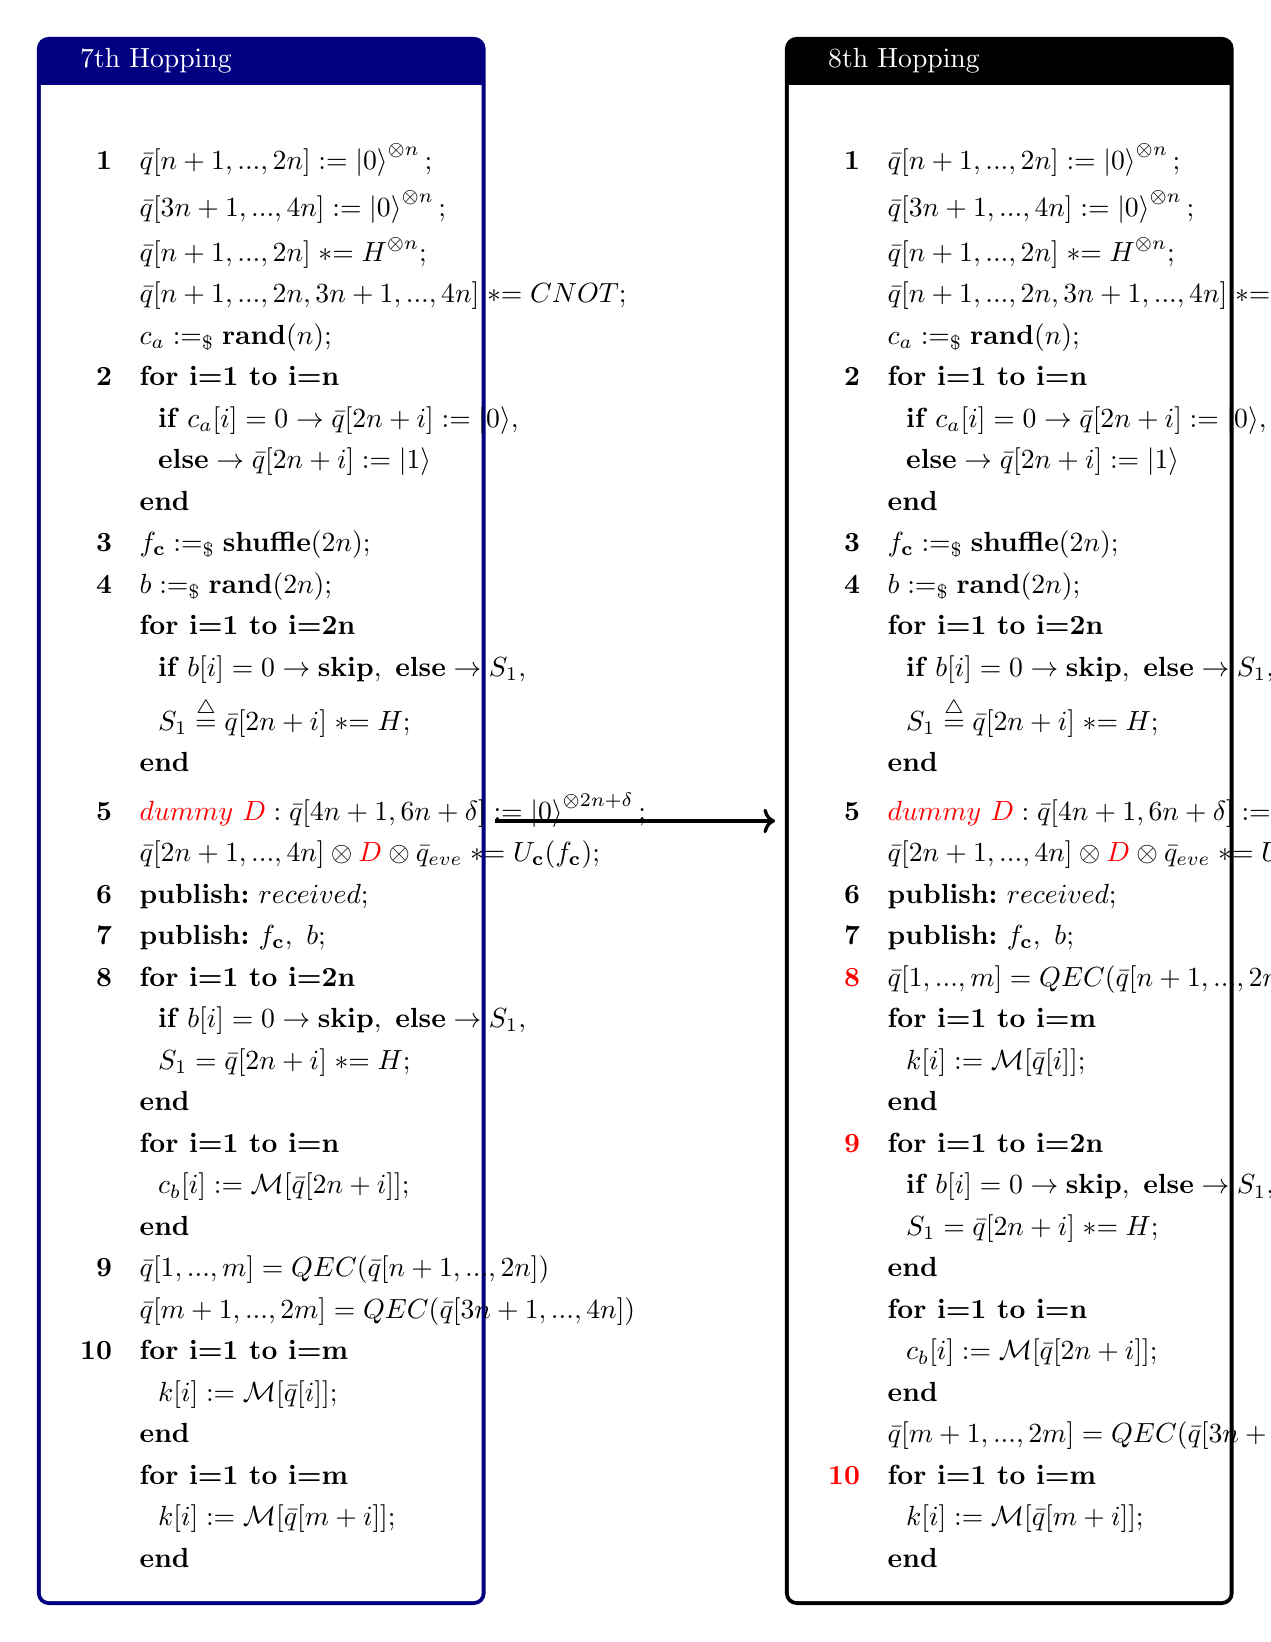
\begin{tikzpicture}[remember picture]

% Left box
\node[anchor=north west] (leftbox) at (0,0) {
\begin{minipage}[t]{0.47\textwidth}
\begin{tcolorbox}[colframe=blue!50!black, colback=white, title=7th Hopping, width=\textwidth]
\begin{align*}
    \textbf{{1}} \quad &\bar{q}[n+1,...,2n] := \ket{0}^{\otimes n};\\
    &\bar{q}[3n+1,...,4n] := \ket{0}^{\otimes n};\\
    \quad &\bar{q}[n+1,...,2n] \asteq H^{\otimes n}; \\
    &\bar{q}[n+1,...,2n,3n+1,...,4n] \asteq CNOT; \\
    & c_a :=_\$ \textbf{rand}(n); \\ 
    \textbf{{2}} \quad &\textbf{for i=1 to i=n}\\
    &~~ \textbf{if }  c_a[i] = 0 \rightarrow \bar{q}[2n+i] := |0\rangle,\\ &~~\textbf{else}   \rightarrow \bar{q}[2n+i] := |1\rangle\\
    &\textbf{end}\ \\
    \textbf{{3}} \quad & f_{\textbf{c}}:=_\$\textbf{shuffle}(2n); \\
    \textbf{{4}} \quad & b :=_\$ \textbf{rand}(2n); \\
    &\textbf{for i=1 to i=2n}\\
    &~~ \textbf{if }  b[i] = 0 \rightarrow \textbf{skip},~\textbf{else}\rightarrow S_{1} ,\\
    &~~ S_{1}\stackrel{\triangle}{=}\bar{q}[2n+i] \asteq H ;\\
    &\textbf{end}\\
    \textbf{{5}} \quad & \textcolor{red}{dummy~D}: \bar{q}[4n+1,6n+\delta]:=\ket{0}^{\otimes 2n+\delta};\\     &\bar{q}[2n+1,...,4n]\otimes \textcolor{red}{D} \otimes \bar{q}_{eve} \asteq U_{\textbf{c}}(f_{\textbf{c}}); \\
    \textbf{{6}} \quad & \textbf{publish:}~ received;\\
    \textbf{{7}} \quad & \textbf{publish:}~ f_{\textbf{c}},~b;\\
    \textbf{{8}} \quad & \textbf{for i=1 to i=2n}\\
    &~~ \textbf{if }  b[i] = 0 \rightarrow \textbf{skip},~\textbf{else}\rightarrow S_{1} ,\\
    &~~ S_{1}=\bar{q}[2n+i] \asteq H ;\\
    &\textbf{end}\\
    \quad & \textbf{for~i=1~to~i=n}\\
    &~~ c_b[i]:= \mathcal{M} [\bar{q}[2n+i]];\\
    &\textbf{end}\\
    \textbf{9} \quad & \bar{q}[1,...,m]=QEC(\bar{q}[n+1,...,2n])\\
    \quad & \bar{q}[m+1,...,2m]=QEC(\bar{q}[3n+1,...,4n])\\
    \textbf{10} \quad & \textbf{for~i=1~to~i=m}\\
    &~~ k[i]:= \mathcal{M} [\bar{q}[i]];\\
    &\textbf{end}
    \\
    & \textbf{for~i=1~to~i=m}\\
    &~~ k[i]:= \mathcal{M} [\bar{q}[m+i]];\\
    &\textbf{end}
\end{align*}
\end{tcolorbox}
\end{minipage}
};

% Right box
\node[anchor=north west] (rightbox) at (9.5,0) {
\begin{minipage}[t]{0.47\textwidth}
\begin{tcolorbox}[colframe=black!50!black, colback=white, title=8th Hopping, width=\textwidth]
\begin{align*}
    \textbf{{1}} \quad &\bar{q}[n+1,...,2n] := \ket{0}^{\otimes n};\\
    &\bar{q}[3n+1,...,4n] := \ket{0}^{\otimes n};\\
    \quad &\bar{q}[n+1,...,2n] \asteq H^{\otimes n}; \\
    &\bar{q}[n+1,...,2n,3n+1,...,4n] \asteq CNOT; \\
    & c_a :=_\$ \textbf{rand}(n); \\ 
    \textbf{{2}} \quad &\textbf{for i=1 to i=n}\\
    &~~ \textbf{if }  c_a[i] = 0 \rightarrow \bar{q}[2n+i] := |0\rangle,\\ &~~\textbf{else}   \rightarrow \bar{q}[2n+i] := |1\rangle\\
    &\textbf{end}\ \\
    \textbf{{3}} \quad & f_{\textbf{c}}:=_\$\textbf{shuffle}(2n); \\
    \textbf{{4}} \quad & b :=_\$ \textbf{rand}(2n); \\
    &\textbf{for i=1 to i=2n}\\
    &~~ \textbf{if }  b[i] = 0 \rightarrow \textbf{skip},~\textbf{else}\rightarrow S_{1} ,\\
    &~~ S_{1}\stackrel{\triangle}{=}\bar{q}[2n+i] \asteq H ;\\
    &\textbf{end}\\
    \textbf{{5}} \quad & \textcolor{red}{dummy~D}: \bar{q}[4n+1,6n+\delta]:=\ket{0}^{\otimes 2n+\delta};\\     &\bar{q}[2n+1,...,4n]\otimes \textcolor{red}{D} \otimes \bar{q}_{eve} \asteq U_{\textbf{c}}(f_{\textbf{c}}); \\
    \textbf{{6}} \quad & \textbf{publish:}~ received;\\
    \textbf{{7}} \quad & \textbf{publish:}~ f_{\textbf{c}},~b;\\
    \textbf{\textcolor{red}{8}} \quad & \bar{q}[1,...,m]=QEC(\bar{q}[n+1,...,2n])\\
    & \textbf{for~i=1~to~i=m}\\
    &~~ k[i]:= \mathcal{M} [\bar{q}[i]];\\
    &\textbf{end}\\
    \textbf{\textcolor{red}{9}} \quad & \textbf{for i=1 to i=2n}\\
    &~~ \textbf{if }  b[i] = 0 \rightarrow \textbf{skip},~\textbf{else}\rightarrow S_{1} ,\\
    &~~ S_{1}=\bar{q}[2n+i] \asteq H ;\\
    &\textbf{end}\\
    \quad & \textbf{for~i=1~to~i=n}\\
    &~~ c_b[i]:= \mathcal{M} [\bar{q}[2n+i]];\\
    &\textbf{end}\\
    \quad & \bar{q}[m+1,...,2m]=QEC(\bar{q}[3n+1,...,4n])\\
    \textbf{\textcolor{red}{10}} \quad 
    & \textbf{for~i=1~to~i=m}\\
    &~~ k[i]:= \mathcal{M} [\bar{q}[m+i]];\\
    &\textbf{end}
\end{align*}
\end{tcolorbox}
\end{minipage}
};

% Draw arrow between boxes
\draw[->, very thick] (leftbox.east) -- node[above]{} (rightbox.west);

\end{tikzpicture}
\newpage

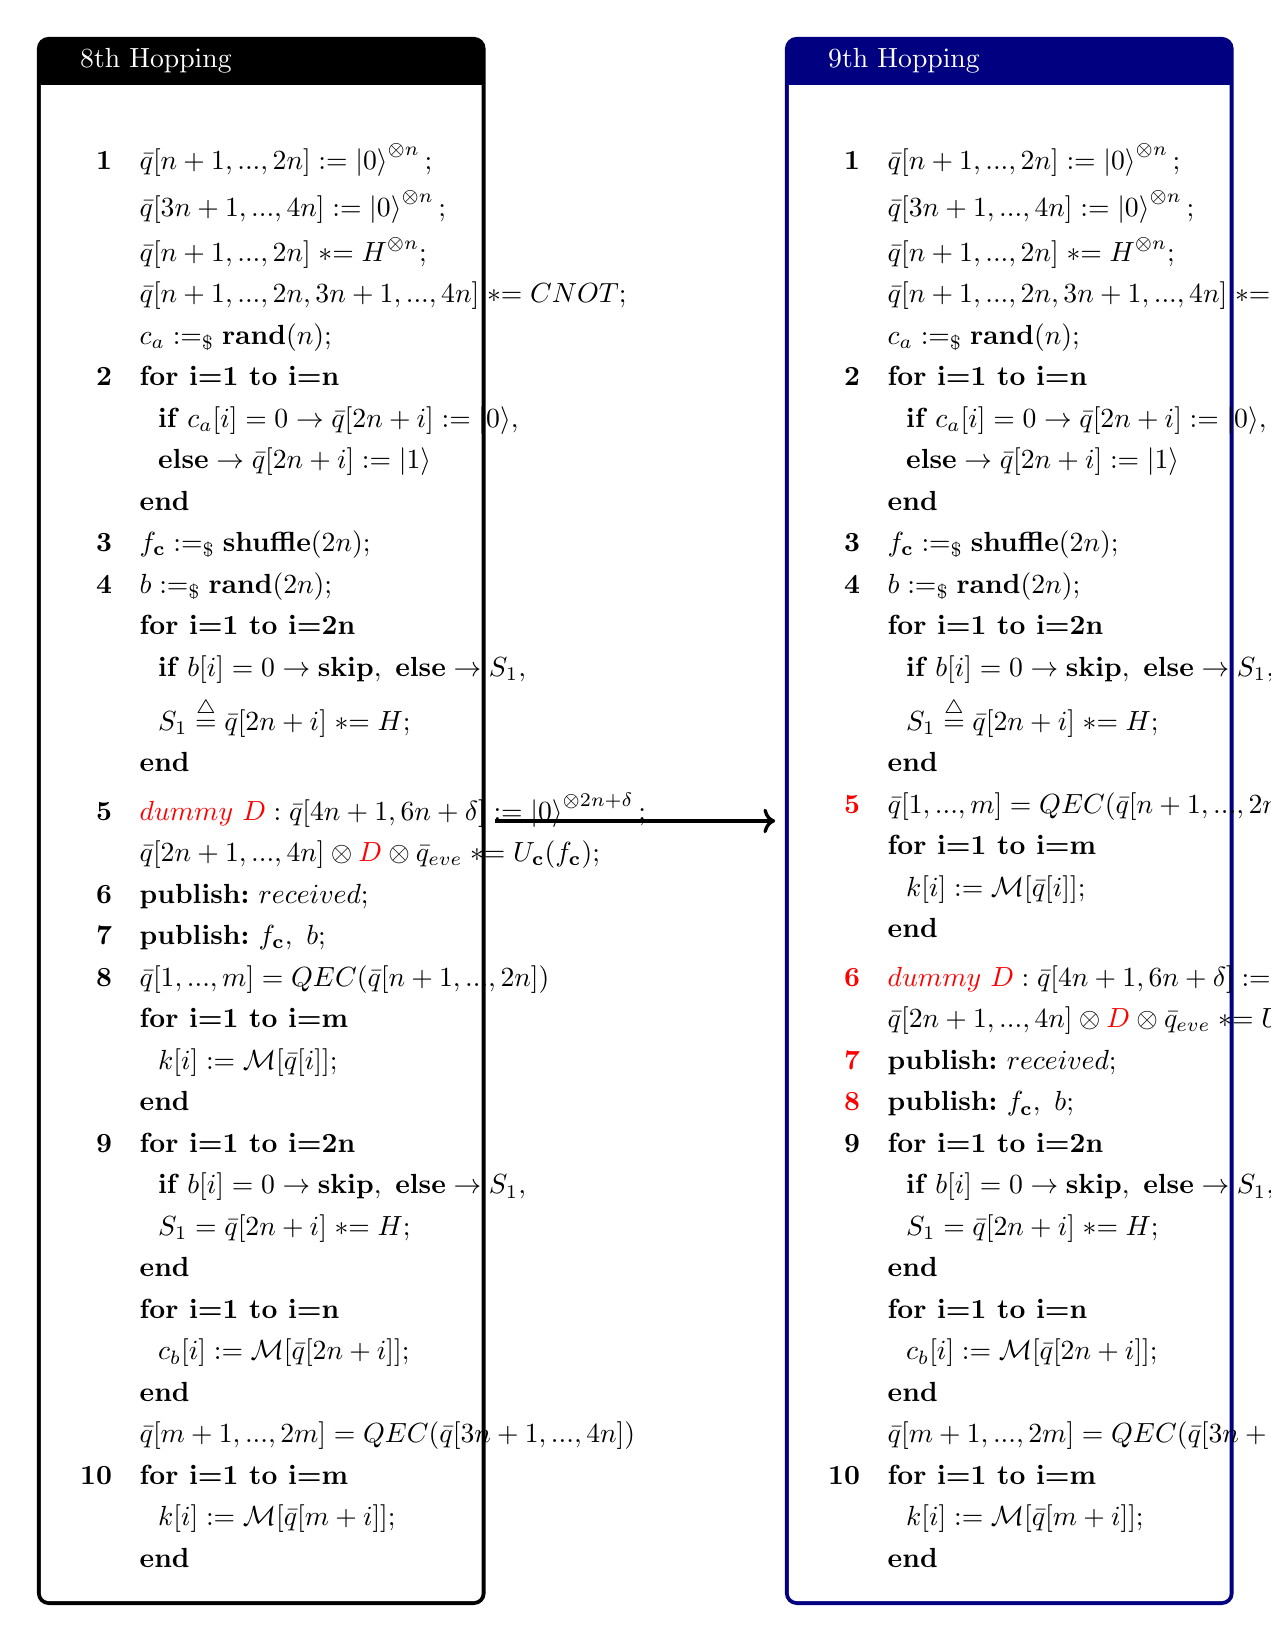
\begin{tikzpicture}[remember picture]

% Left box
\node[anchor=north west] (leftbox) at (0,0) {
\begin{minipage}[t]{0.47\textwidth}
\begin{tcolorbox}[colframe=black!75!black, colback=white, title=8th Hopping, width=\textwidth]
\begin{align*}
    \textbf{{1}} \quad &\bar{q}[n+1,...,2n] := \ket{0}^{\otimes n};\\
    &\bar{q}[3n+1,...,4n] := \ket{0}^{\otimes n};\\
    \quad &\bar{q}[n+1,...,2n] \asteq H^{\otimes n}; \\
    &\bar{q}[n+1,...,2n,3n+1,...,4n] \asteq CNOT; \\
    & c_a :=_\$ \textbf{rand}(n); \\ 
    \textbf{{2}} \quad &\textbf{for i=1 to i=n}\\
    &~~ \textbf{if }  c_a[i] = 0 \rightarrow \bar{q}[2n+i] := |0\rangle,\\ &~~\textbf{else}   \rightarrow \bar{q}[2n+i] := |1\rangle\\
    &\textbf{end}\ \\
    \textbf{{3}} \quad & f_{\textbf{c}}:=_\$\textbf{shuffle}(2n); \\
    \textbf{{4}} \quad & b :=_\$ \textbf{rand}(2n); \\
    &\textbf{for i=1 to i=2n}\\
    &~~ \textbf{if }  b[i] = 0 \rightarrow \textbf{skip},~\textbf{else}\rightarrow S_{1} ,\\
    &~~ S_{1}\stackrel{\triangle}{=}\bar{q}[2n+i] \asteq H ;\\
    &\textbf{end}\\
    \textbf{{5}} \quad & \textcolor{red}{dummy~D}: \bar{q}[4n+1,6n+\delta]:=\ket{0}^{\otimes 2n+\delta};\\     &\bar{q}[2n+1,...,4n]\otimes \textcolor{red}{D} \otimes \bar{q}_{eve} \asteq U_{\textbf{c}}(f_{\textbf{c}}); \\
    \textbf{{6}} \quad & \textbf{publish:}~ received;\\
    \textbf{{7}} \quad & \textbf{publish:}~ f_{\textbf{c}},~b;\\
    \textbf{{8}} \quad & \bar{q}[1,...,m]=QEC(\bar{q}[n+1,...,2n])\\
    & \textbf{for~i=1~to~i=m}\\
    &~~ k[i]:= \mathcal{M} [\bar{q}[i]];\\
    &\textbf{end}\\
    \textbf{{9}} \quad & \textbf{for i=1 to i=2n}\\
    &~~ \textbf{if }  b[i] = 0 \rightarrow \textbf{skip},~\textbf{else}\rightarrow S_{1} ,\\
    &~~ S_{1}=\bar{q}[2n+i] \asteq H ;\\
    &\textbf{end}\\
    \quad & \textbf{for~i=1~to~i=n}\\
    &~~ c_b[i]:= \mathcal{M} [\bar{q}[2n+i]];\\
    &\textbf{end}\\
    \quad & \bar{q}[m+1,...,2m]=QEC(\bar{q}[3n+1,...,4n])\\
    \textbf{{10}} \quad 
    & \textbf{for~i=1~to~i=m}\\
    &~~ k[i]:= \mathcal{M} [\bar{q}[m+i]];\\
    &\textbf{end}
\end{align*}
\end{tcolorbox}
\end{minipage}
};

% Right box
\node[anchor=north west] (rightbox) at (9.5,0) {
\begin{minipage}[t]{0.47\textwidth}
\begin{tcolorbox}[colframe=blue!50!black, colback=white, title=9th Hopping, width=\textwidth]
\begin{align*}
    \textbf{{1}} \quad &\bar{q}[n+1,...,2n] := \ket{0}^{\otimes n};\\
    &\bar{q}[3n+1,...,4n] := \ket{0}^{\otimes n};\\
    \quad &\bar{q}[n+1,...,2n] \asteq H^{\otimes n}; \\
    &\bar{q}[n+1,...,2n,3n+1,...,4n] \asteq CNOT; \\
    & c_a :=_\$ \textbf{rand}(n); \\ 
    \textbf{{2}} \quad &\textbf{for i=1 to i=n}\\
    &~~ \textbf{if }  c_a[i] = 0 \rightarrow \bar{q}[2n+i] := |0\rangle,\\ &~~\textbf{else}   \rightarrow \bar{q}[2n+i] := |1\rangle\\
    &\textbf{end}\ \\
    \textbf{{3}} \quad & f_{\textbf{c}}:=_\$\textbf{shuffle}(2n); \\
    \textbf{{4}} \quad & b :=_\$ \textbf{rand}(2n); \\
    &\textbf{for i=1 to i=2n}\\
    &~~ \textbf{if }  b[i] = 0 \rightarrow \textbf{skip},~\textbf{else}\rightarrow S_{1} ,\\
    &~~ S_{1}\stackrel{\triangle}{=}\bar{q}[2n+i] \asteq H ;\\
    &\textbf{end}\\
    \textbf{\textcolor{red}{5}} \quad & \bar{q}[1,...,m]=QEC(\bar{q}[n+1,...,2n])\\ \quad & \textbf{for~i=1~to~i=m}\\
    &~~ k[i]:= \mathcal{M} [\bar{q}[i]];\\
    &\textbf{end}\\
    \textbf{\textcolor{red}{6}} \quad & \textcolor{red}{dummy~D}: \bar{q}[4n+1,6n+\delta]:=\ket{0}^{\otimes 2n+\delta};\\     &\bar{q}[2n+1,...,4n]\otimes \textcolor{red}{D} \otimes \bar{q}_{eve} \asteq U_{\textbf{c}}(f_{\textbf{c}}); \\
    \textbf{\textcolor{red}{7}} \quad & \textbf{publish:}~ received;\\
    \textbf{\textcolor{red}{8}} \quad & \textbf{publish:}~ f_{\textbf{c}},~b;\\
    \textbf{{9}} \quad & \textbf{for i=1 to i=2n}\\
    &~~ \textbf{if }  b[i] = 0 \rightarrow \textbf{skip},~\textbf{else}\rightarrow S_{1} ,\\
    &~~ S_{1}=\bar{q}[2n+i] \asteq H ;\\
    &\textbf{end}\\
    \quad & \textbf{for~i=1~to~i=n}\\
    &~~ c_b[i]:= \mathcal{M} [\bar{q}[2n+i]];\\
    &\textbf{end}\\
    \quad & \bar{q}[m+1,...,2m]=QEC(\bar{q}[3n+1,...,4n])\\
    \textbf{{10}} \quad 
    & \textbf{for~i=1~to~i=m}\\
    &~~ k[i]:= \mathcal{M} [\bar{q}[m+i]];\\
    &\textbf{end}
\end{align*}
\end{tcolorbox}
\end{minipage}
};

% Draw arrow between boxes
\draw[->, very thick] (leftbox.east) -- node[above]{} (rightbox.west);

\end{tikzpicture}
\newpage

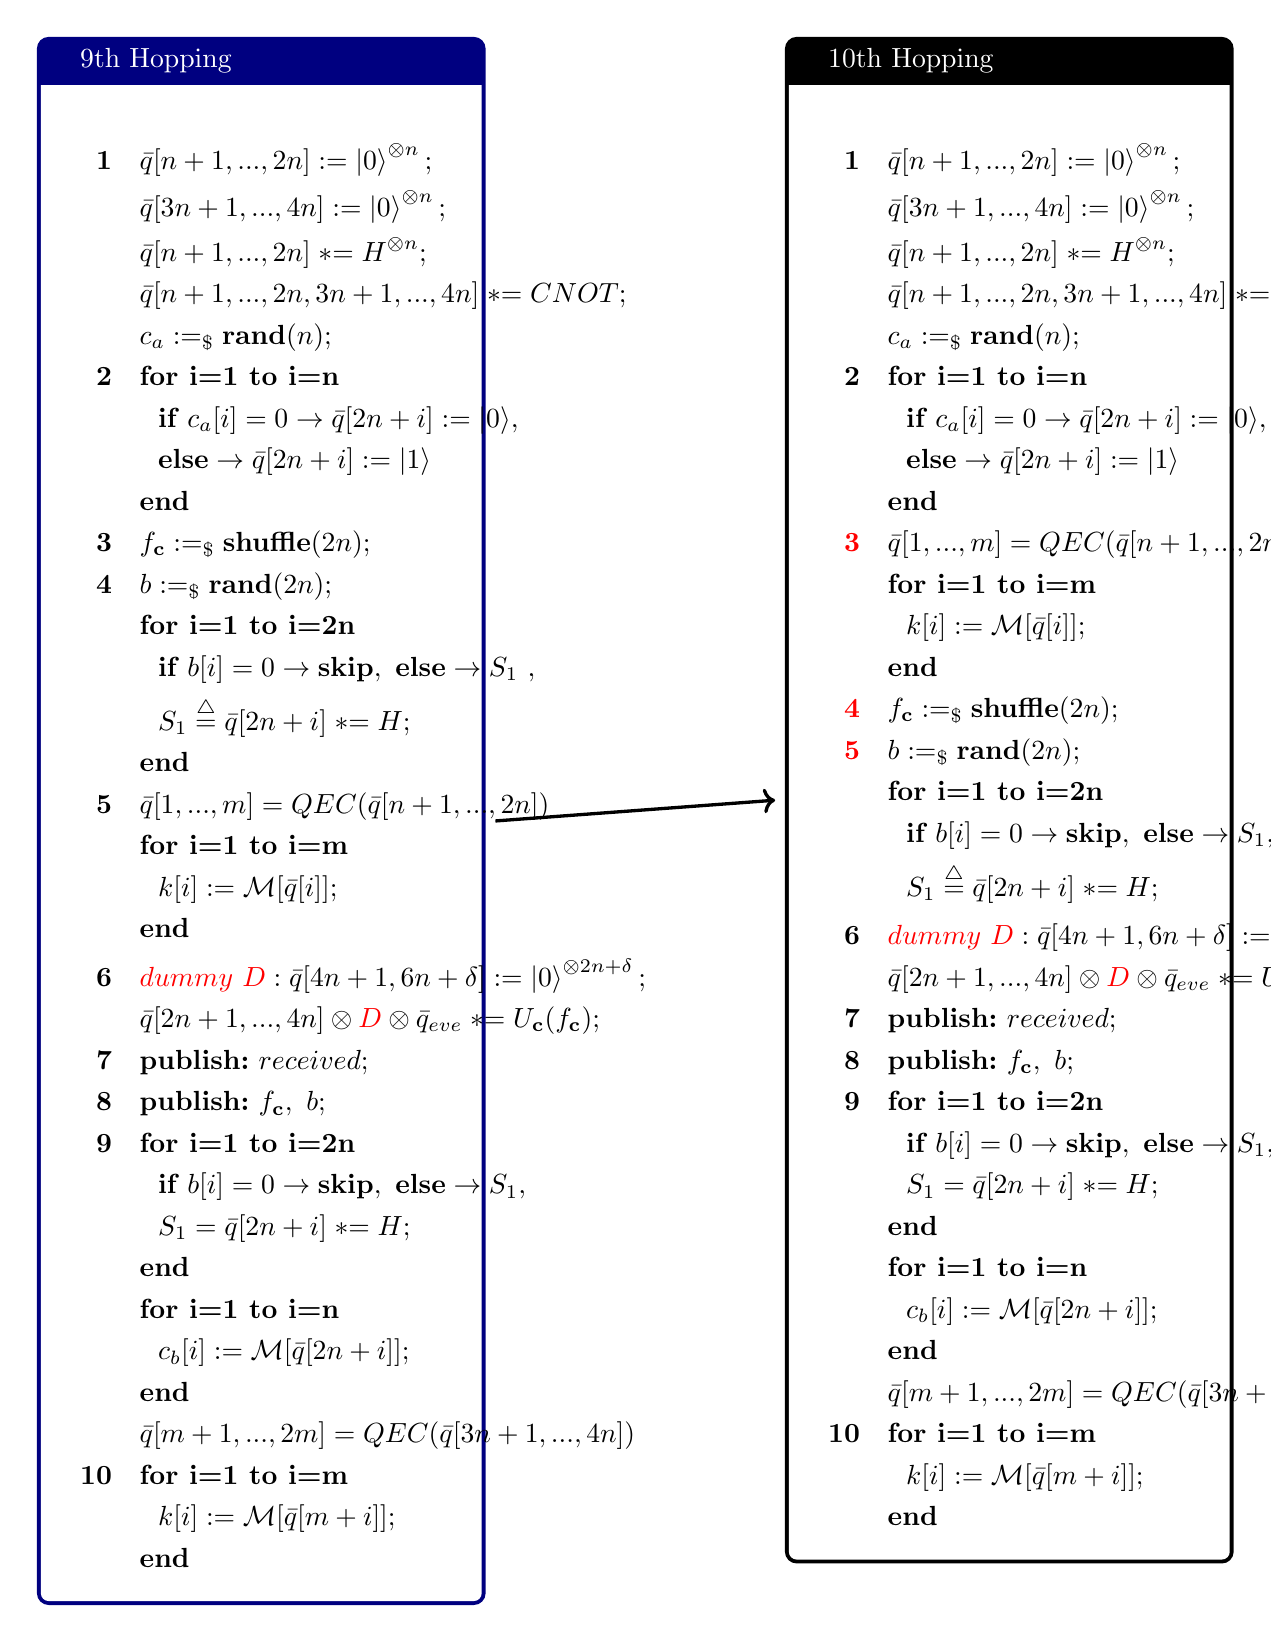
\begin{tikzpicture}[remember picture]

% Left box
\node[anchor=north west] (leftbox) at (0,0) {
\begin{minipage}[t]{0.47\textwidth}
\begin{tcolorbox}[colframe=blue!50!black, colback=white, title=9th Hopping, width=\textwidth]
\begin{align*}
    \textbf{{1}} \quad &\bar{q}[n+1,...,2n] := \ket{0}^{\otimes n};\\
    &\bar{q}[3n+1,...,4n] := \ket{0}^{\otimes n};\\
    \quad &\bar{q}[n+1,...,2n] \asteq H^{\otimes n}; \\
    &\bar{q}[n+1,...,2n,3n+1,...,4n] \asteq CNOT; \\
    & c_a :=_\$ \textbf{rand}(n); \\ 
    \textbf{{2}} \quad &\textbf{for i=1 to i=n}\\
    &~~ \textbf{if }  c_a[i] = 0 \rightarrow \bar{q}[2n+i] := |0\rangle,\\ &~~\textbf{else}   \rightarrow \bar{q}[2n+i] := |1\rangle\\
    &\textbf{end}\ \\
    \textbf{{3}} \quad & f_{\textbf{c}}:=_\$\textbf{shuffle}(2n); \\
    \textbf{{4}} \quad & b :=_\$ \textbf{rand}(2n); \\
    &\textbf{for i=1 to i=2n}\\
    &~~ \textbf{if }  b[i] = 0 \rightarrow \textbf{skip},~\textbf{else}\rightarrow S_1~,\\
    &~~ S_{1}\stackrel{\triangle}{=}\bar{q}[2n+i] \asteq H ;\\
    &\textbf{end}\\
    \textbf{{5}} \quad & \bar{q}[1,...,m]=QEC(\bar{q}[n+1,...,2n])\\ \quad & \textbf{for~i=1~to~i=m}\\
    &~~ k[i]:= \mathcal{M} [\bar{q}[i]];\\
    &\textbf{end}\\
    \textbf{{6}} \quad & \textcolor{red}{dummy~D}: \bar{q}[4n+1,6n+\delta]:=\ket{0}^{\otimes 2n+\delta};\\     &\bar{q}[2n+1,...,4n]\otimes \textcolor{red}{D} \otimes \bar{q}_{eve} \asteq U_{\textbf{c}}(f_{\textbf{c}}); \\
    \textbf{{7}} \quad & \textbf{publish:}~ received;\\
    \textbf{{8}} \quad & \textbf{publish:}~ f_{\textbf{c}},~b;\\
    \textbf{{9}} \quad & \textbf{for i=1 to i=2n}\\
    &~~ \textbf{if }  b[i] = 0 \rightarrow \textbf{skip},~\textbf{else}\rightarrow S_{1} ,\\
    &~~ S_{1}=\bar{q}[2n+i] \asteq H ;\\
    &\textbf{end}\\
    \quad & \textbf{for~i=1~to~i=n}\\
    &~~ c_b[i]:= \mathcal{M} [\bar{q}[2n+i]];\\
    &\textbf{end}\\
    \quad & \bar{q}[m+1,...,2m]=QEC(\bar{q}[3n+1,...,4n])\\
    \textbf{{10}} \quad 
    & \textbf{for~i=1~to~i=m}\\
    &~~ k[i]:= \mathcal{M} [\bar{q}[m+i]];\\
    &\textbf{end}
\end{align*}
\end{tcolorbox}
\end{minipage}
};

% Right box
\node[anchor=north west] (rightbox) at (9.5,0) {
\begin{minipage}[t]{0.47\textwidth}
\begin{tcolorbox}[colframe=black!50!black, colback=white, title=10th Hopping, width=\textwidth]
\begin{align*}
    \textbf{{1}} \quad &\bar{q}[n+1,...,2n] := \ket{0}^{\otimes n};\\
    &\bar{q}[3n+1,...,4n] := \ket{0}^{\otimes n};\\
    \quad &\bar{q}[n+1,...,2n] \asteq H^{\otimes n}; \\
    &\bar{q}[n+1,...,2n,3n+1,...,4n] \asteq CNOT; \\
    & c_a :=_\$ \textbf{rand}(n); \\ 
    \textbf{{2}} \quad &\textbf{for i=1 to i=n}\\
    &~~ \textbf{if }  c_a[i] = 0 \rightarrow \bar{q}[2n+i] := |0\rangle,\\ &~~\textbf{else}   \rightarrow \bar{q}[2n+i] := |1\rangle\\
    &\textbf{end}\ \\
    \textbf{\textcolor{red}{3}} \quad & \bar{q}[1,...,m]=QEC(\bar{q}[n+1,...,2n])\\
    \quad & \textbf{for~i=1~to~i=m}\\
    &~~ k[i]:= \mathcal{M} [\bar{q}[i]];\\
    &\textbf{end}\\
    \textbf{\textcolor{red}{4}} \quad & f_{\textbf{c}}:=_\$\textbf{shuffle}(2n); \\
    \textbf{\textcolor{red}{5}} \quad & b :=_\$ \textbf{rand}(2n); \\
    &\textbf{for i=1 to i=2n}\\
    &~~ \textbf{if }  b[i] = 0 \rightarrow \textbf{skip},~\textbf{else}\rightarrow S_{1} ,\\
    &~~ S_{1}\stackrel{\triangle}{=}\bar{q}[2n+i] \asteq H ;\\
    \textbf{{6}} \quad & \textcolor{red}{dummy~D}: \bar{q}[4n+1,6n+\delta]:=\ket{0}^{\otimes 2n+\delta};\\     &\bar{q}[2n+1,...,4n]\otimes \textcolor{red}{D} \otimes \bar{q}_{eve} \asteq U_{\textbf{c}}(f_{\textbf{c}}); \\
    \textbf{{7}} \quad & \textbf{publish:}~ received;\\
    \textbf{{8}} \quad & \textbf{publish:}~ f_{\textbf{c}},~b;\\
    \textbf{{9}} \quad & \textbf{for i=1 to i=2n}\\
    &~~ \textbf{if }  b[i] = 0 \rightarrow \textbf{skip},~\textbf{else}\rightarrow S_{1} ,\\
    &~~ S_{1}=\bar{q}[2n+i] \asteq H ;\\
    &\textbf{end}\\
    \quad & \textbf{for~i=1~to~i=n}\\
    &~~ c_b[i]:= \mathcal{M} [\bar{q}[2n+i]];\\
    &\textbf{end}\\
    \quad & \bar{q}[m+1,...,2m]=QEC(\bar{q}[3n+1,...,4n])\\
    \textbf{{10}} \quad 
    & \textbf{for~i=1~to~i=m}\\
    &~~ k[i]:= \mathcal{M} [\bar{q}[m+i]];\\
    &\textbf{end}
\end{align*}
\end{tcolorbox}
\end{minipage}
};

% Draw arrow between boxes
\draw[->, very thick] (leftbox.east) -- node[above]{} (rightbox.west);

\end{tikzpicture}
\newpage

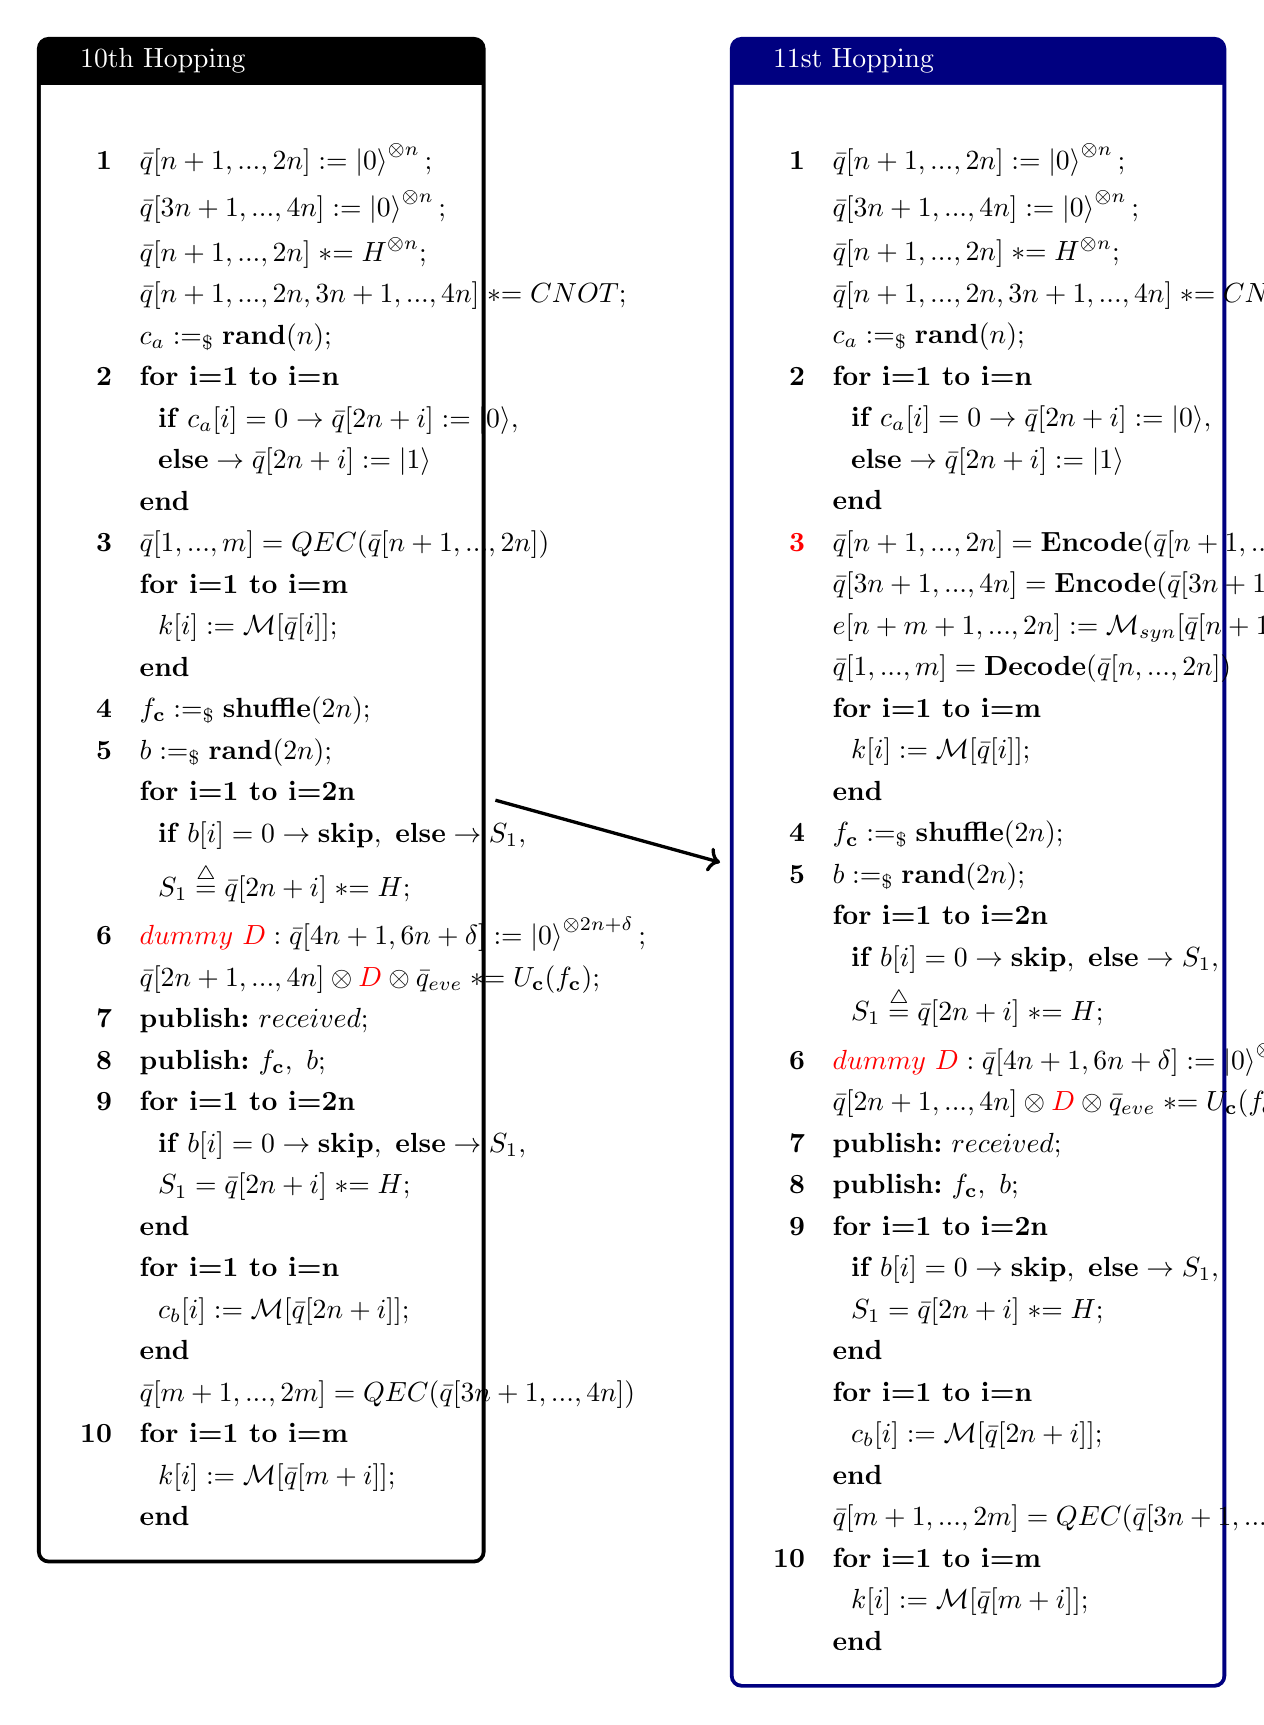
\begin{tikzpicture}[remember picture]

% Left box
\node[anchor=north west] (leftbox) at (0,0) {
\begin{minipage}[t]{0.47\textwidth}
\begin{tcolorbox}[colframe=black!75!black, colback=white, title=10th Hopping, width=\textwidth]
\begin{align*}
    \textbf{{1}} \quad &\bar{q}[n+1,...,2n] := \ket{0}^{\otimes n};\\
    &\bar{q}[3n+1,...,4n] := \ket{0}^{\otimes n};\\
    \quad &\bar{q}[n+1,...,2n] \asteq H^{\otimes n}; \\
    &\bar{q}[n+1,...,2n,3n+1,...,4n] \asteq CNOT; \\
    & c_a :=_\$ \textbf{rand}(n); \\ 
    \textbf{{2}} \quad &\textbf{for i=1 to i=n}\\
    &~~ \textbf{if }  c_a[i] = 0 \rightarrow \bar{q}[2n+i] := |0\rangle,\\ &~~\textbf{else}   \rightarrow \bar{q}[2n+i] := |1\rangle\\
    &\textbf{end}\ \\
    \textbf{{3}} \quad & \bar{q}[1,...,m]=QEC(\bar{q}[n+1,...,2n])\\
    \quad & \textbf{for~i=1~to~i=m}\\
    &~~ k[i]:= \mathcal{M} [\bar{q}[i]];\\
    &\textbf{end}\\
    \textbf{{4}} \quad & f_{\textbf{c}}:=_\$\textbf{shuffle}(2n); \\
    \textbf{{5}} \quad & b :=_\$ \textbf{rand}(2n); \\
    &\textbf{for i=1 to i=2n}\\
    &~~ \textbf{if }  b[i] = 0 \rightarrow \textbf{skip},~\textbf{else}\rightarrow S_{1} ,\\
    &~~ S_{1}\stackrel{\triangle}{=}\bar{q}[2n+i] \asteq H ;\\
    \textbf{{6}} \quad & \textcolor{red}{dummy~D}: \bar{q}[4n+1,6n+\delta]:=\ket{0}^{\otimes 2n+\delta};\\     &\bar{q}[2n+1,...,4n]\otimes \textcolor{red}{D} \otimes \bar{q}_{eve} \asteq U_{\textbf{c}}(f_{\textbf{c}}); \\
    \textbf{{7}} \quad & \textbf{publish:}~ received;\\
    \textbf{{8}} \quad & \textbf{publish:}~ f_{\textbf{c}},~b;\\
    \textbf{{9}} \quad & \textbf{for i=1 to i=2n}\\
    &~~ \textbf{if }  b[i] = 0 \rightarrow \textbf{skip},~\textbf{else}\rightarrow S_{1} ,\\
    &~~ S_{1}=\bar{q}[2n+i] \asteq H ;\\
    &\textbf{end}\\
    \quad & \textbf{for~i=1~to~i=n}\\
    &~~ c_b[i]:= \mathcal{M} [\bar{q}[2n+i]];\\
    &\textbf{end}\\
    \quad & \bar{q}[m+1,...,2m]=QEC(\bar{q}[3n+1,...,4n])\\
    \textbf{{10}} \quad 
    & \textbf{for~i=1~to~i=m}\\
    &~~ k[i]:= \mathcal{M} [\bar{q}[m+i]];\\
    &\textbf{end}
\end{align*}
\end{tcolorbox}
\end{minipage}
};

% Right box
\node[anchor=north west] (rightbox) at (8.8,0) {
\begin{minipage}[t]{0.52\textwidth}
\begin{tcolorbox}[colframe=blue!50!black, colback=white, title=11st Hopping, width=\textwidth]
\begin{align*}
    \textbf{{1}} \quad &\bar{q}[n+1,...,2n] := \ket{0}^{\otimes n};\\
    &\bar{q}[3n+1,...,4n] := \ket{0}^{\otimes n};\\
    \quad &\bar{q}[n+1,...,2n] \asteq H^{\otimes n}; \\
    &\bar{q}[n+1,...,2n,3n+1,...,4n] \asteq CNOT; \\
    & c_a :=_\$ \textbf{rand}(n); \\ 
    \textbf{{2}} \quad &\textbf{for i=1 to i=n}\\
    &~~ \textbf{if }  c_a[i] = 0 \rightarrow \bar{q}[2n+i] := |0\rangle,\\ &~~\textbf{else}   \rightarrow \bar{q}[2n+i] := |1\rangle\\
    &\textbf{end}\ \\
    \textbf{\textcolor{red}{3}} \quad &\bar{q}[n+1,...,2n]=\textbf{Encode}(\bar{q}[n+1,...,n+m])\\
    &\bar{q}[3n+1,...,4n]=\textbf{Encode}(\bar{q}[3n+1,...,3n+m])\\
    & e[n+m+1,...,2n]:=\mathcal{M}_{syn} [\bar{q}[n+1,...,2n]];\\
    & \bar{q}[1,...,m]=\textbf{Decode}(\bar{q}[n,...,2n])\\
    \quad & \textbf{for~i=1~to~i=m}\\
    &~~ k[i]:= \mathcal{M} [\bar{q}[i]];\\
    &\textbf{end}\\
    \textbf{{4}} \quad & f_{\textbf{c}}:=_\$\textbf{shuffle}(2n); \\
    \textbf{{5}} \quad & b :=_\$ \textbf{rand}(2n); \\
    &\textbf{for i=1 to i=2n}\\
    &~~ \textbf{if }  b[i] = 0 \rightarrow \textbf{skip},~\textbf{else}\rightarrow S_{1} ,\\
    &~~ S_{1}\stackrel{\triangle}{=}\bar{q}[2n+i] \asteq H ;\\
    \textbf{{6}} \quad & \textcolor{red}{dummy~D}: \bar{q}[4n+1,6n+\delta]:=\ket{0}^{\otimes 2n+\delta};\\     &\bar{q}[2n+1,...,4n]\otimes \textcolor{red}{D} \otimes \bar{q}_{eve} \asteq U_{\textbf{c}}(f_{\textbf{c}}); \\
    \textbf{{7}} \quad & \textbf{publish:}~ received;\\
    \textbf{{8}} \quad & \textbf{publish:}~ f_{\textbf{c}},~b;\\
    \textbf{{9}} \quad & \textbf{for i=1 to i=2n}\\
    &~~ \textbf{if }  b[i] = 0 \rightarrow \textbf{skip},~\textbf{else}\rightarrow S_{1} ,\\
    &~~ S_{1}=\bar{q}[2n+i] \asteq H ;\\
    &\textbf{end}\\
    \quad & \textbf{for~i=1~to~i=n}\\
    &~~ c_b[i]:= \mathcal{M} [\bar{q}[2n+i]];\\
    &\textbf{end}\\
    \quad & \bar{q}[m+1,...,2m]=QEC(\bar{q}[3n+1,...,4n])\\
    \textbf{{10}} \quad 
    & \textbf{for~i=1~to~i=m}\\
    &~~ k[i]:= \mathcal{M} [\bar{q}[m+i]];\\
    &\textbf{end}
\end{align*}
\end{tcolorbox}
\end{minipage}
};

% Draw arrow between boxes
\draw[->, very thick] (leftbox.east) -- node[above]{} (rightbox.west);

\end{tikzpicture}
\newpage

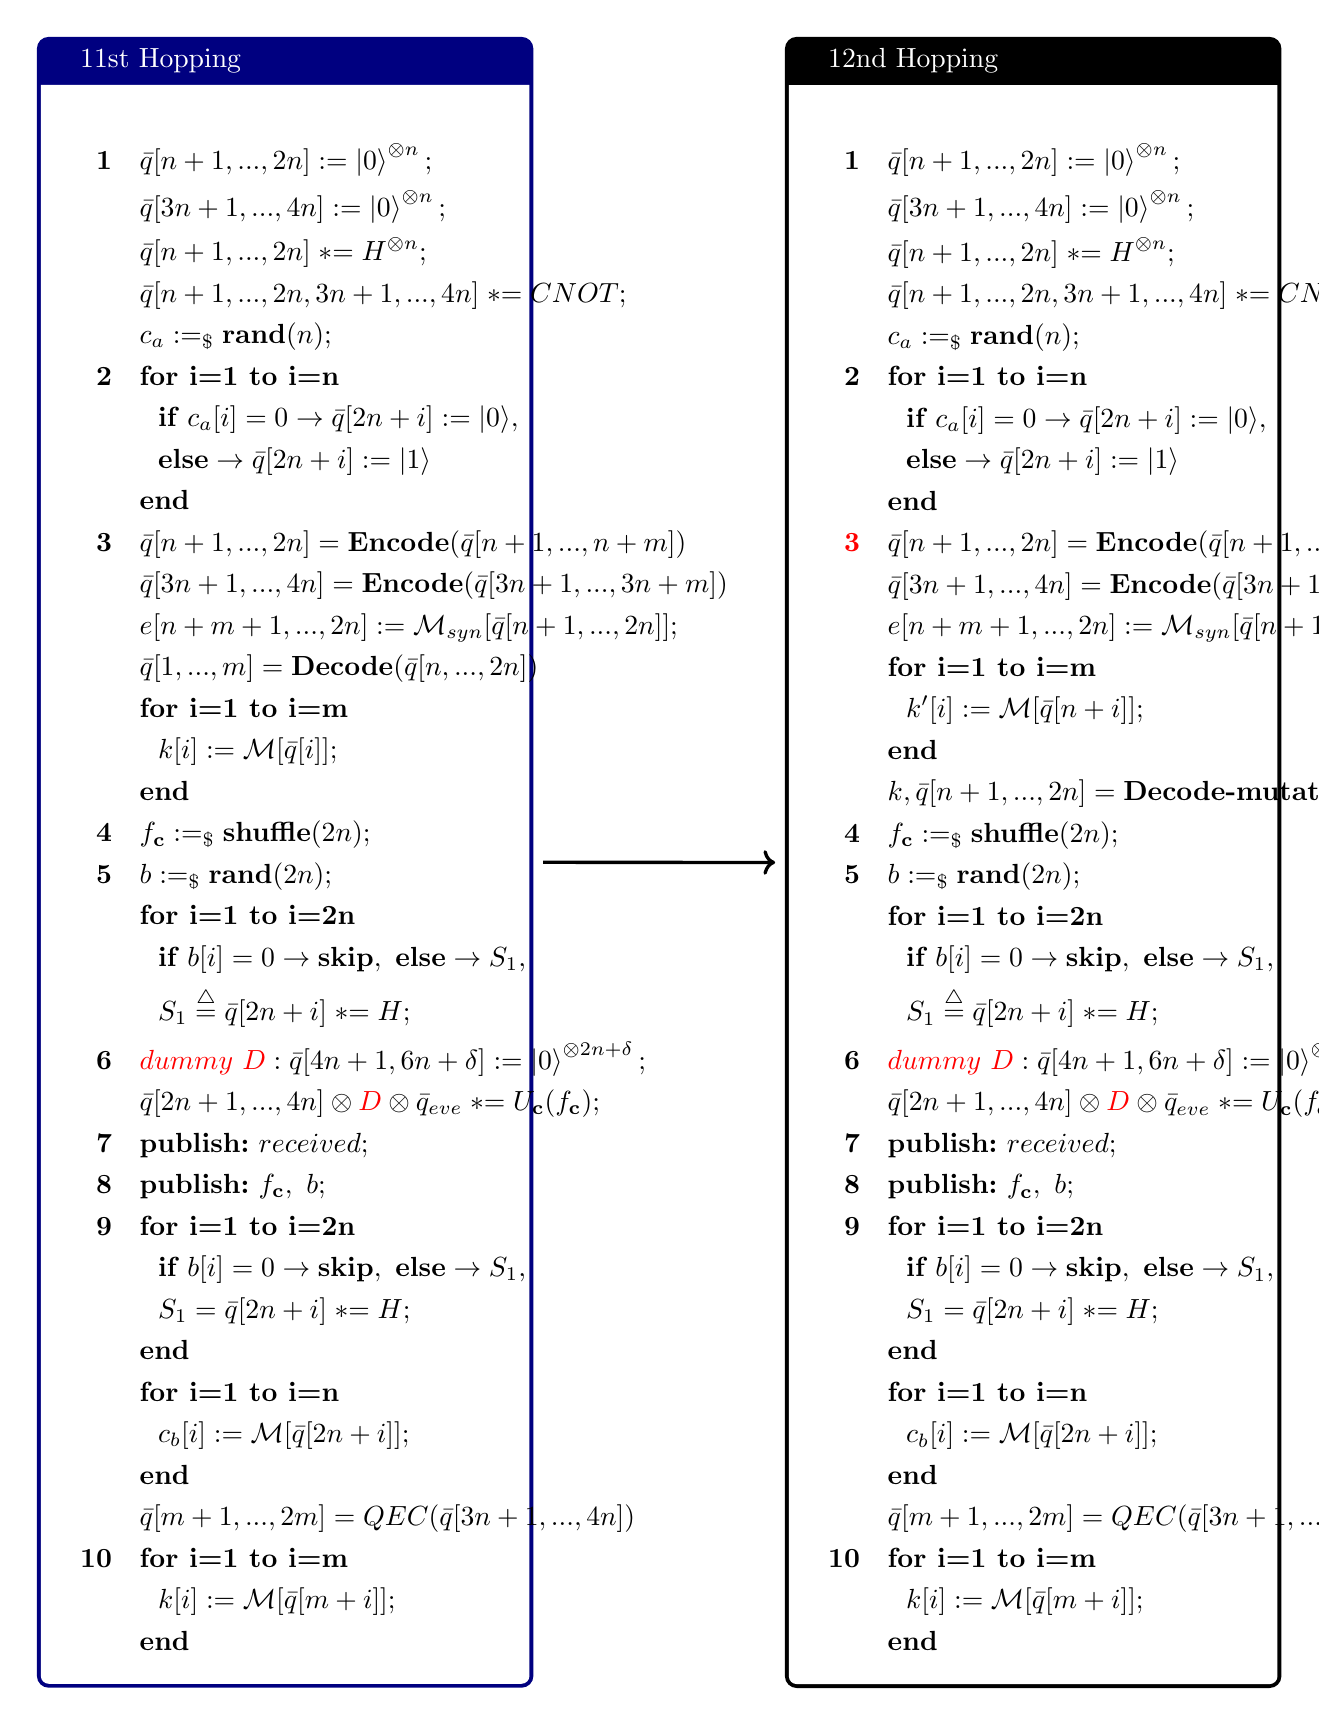
\begin{tikzpicture}[remember picture]

% Left box
\node[anchor=north west] (leftbox) at (0,0) {
\begin{minipage}[t]{0.52\textwidth}
\begin{tcolorbox}[colframe=blue!50!black, colback=white, title=11st Hopping, width=\textwidth]
\begin{align*}
    \textbf{{1}} \quad &\bar{q}[n+1,...,2n] := \ket{0}^{\otimes n};\\
    &\bar{q}[3n+1,...,4n] := \ket{0}^{\otimes n};\\
    \quad &\bar{q}[n+1,...,2n] \asteq H^{\otimes n}; \\
    &\bar{q}[n+1,...,2n,3n+1,...,4n] \asteq CNOT; \\
    & c_a :=_\$ \textbf{rand}(n); \\ 
    \textbf{{2}} \quad &\textbf{for i=1 to i=n}\\
    &~~ \textbf{if }  c_a[i] = 0 \rightarrow \bar{q}[2n+i] := |0\rangle,\\ &~~\textbf{else}   \rightarrow \bar{q}[2n+i] := |1\rangle\\
    &\textbf{end}\ \\
    \textbf{{3}} \quad &\bar{q}[n+1,...,2n]=\textbf{Encode}(\bar{q}[n+1,...,n+m])\\
    &\bar{q}[3n+1,...,4n]=\textbf{Encode}(\bar{q}[3n+1,...,3n+m])\\
    & e[n+m+1,...,2n]:=\mathcal{M}_{syn} [\bar{q}[n+1,...,2n]];\\
    & \bar{q}[1,...,m]=\textbf{Decode}(\bar{q}[n,...,2n])\\
    \quad & \textbf{for~i=1~to~i=m}\\
    &~~ k[i]:= \mathcal{M} [\bar{q}[i]];\\
    &\textbf{end}\\
    \textbf{{4}} \quad & f_{\textbf{c}}:=_\$\textbf{shuffle}(2n); \\
    \textbf{{5}} \quad & b :=_\$ \textbf{rand}(2n); \\
    &\textbf{for i=1 to i=2n}\\
    &~~ \textbf{if }  b[i] = 0 \rightarrow \textbf{skip},~\textbf{else}\rightarrow S_{1} ,\\
    &~~ S_{1}\stackrel{\triangle}{=}\bar{q}[2n+i] \asteq H ;\\
    \textbf{{6}} \quad & \textcolor{red}{dummy~D}: \bar{q}[4n+1,6n+\delta]:=\ket{0}^{\otimes 2n+\delta};\\     &\bar{q}[2n+1,...,4n]\otimes \textcolor{red}{D} \otimes \bar{q}_{eve} \asteq U_{\textbf{c}}(f_{\textbf{c}}); \\
    \textbf{{7}} \quad & \textbf{publish:}~ received;\\
    \textbf{{8}} \quad & \textbf{publish:}~ f_{\textbf{c}},~b;\\
    \textbf{{9}} \quad & \textbf{for i=1 to i=2n}\\
    &~~ \textbf{if }  b[i] = 0 \rightarrow \textbf{skip},~\textbf{else}\rightarrow S_{1} ,\\
    &~~ S_{1}=\bar{q}[2n+i] \asteq H ;\\
    &\textbf{end}\\
    \quad & \textbf{for~i=1~to~i=n}\\
    &~~ c_b[i]:= \mathcal{M} [\bar{q}[2n+i]];\\
    &\textbf{end}\\
    \quad & \bar{q}[m+1,...,2m]=QEC(\bar{q}[3n+1,...,4n])\\
    \textbf{{10}} \quad 
    & \textbf{for~i=1~to~i=m}\\
    &~~ k[i]:= \mathcal{M} [\bar{q}[m+i]];\\
    &\textbf{end}
\end{align*}
\end{tcolorbox}
\end{minipage}
};

% Right box
\node[anchor=north west] (rightbox) at (9.5,0) {
\begin{minipage}[t]{0.52\textwidth}
\begin{tcolorbox}[colframe=black!50!black, colback=white, title=12nd Hopping, width=\textwidth]
\begin{align*}
    \textbf{{1}} \quad &\bar{q}[n+1,...,2n] := \ket{0}^{\otimes n};\\
    &\bar{q}[3n+1,...,4n] := \ket{0}^{\otimes n};\\
    \quad &\bar{q}[n+1,...,2n] \asteq H^{\otimes n}; \\
    &\bar{q}[n+1,...,2n,3n+1,...,4n] \asteq CNOT; \\
    & c_a :=_\$ \textbf{rand}(n); \\ 
    \textbf{{2}} \quad &\textbf{for i=1 to i=n}\\
    &~~ \textbf{if }  c_a[i] = 0 \rightarrow \bar{q}[2n+i] := |0\rangle,\\ &~~\textbf{else}   \rightarrow \bar{q}[2n+i] := |1\rangle\\
    &\textbf{end}\ \\
    \textbf{\textcolor{red}{3}} \quad &\bar{q}[n+1,...,2n]=\textbf{Encode}(\bar{q}[n+1,...,n+m])\\
    &\bar{q}[3n+1,...,4n]=\textbf{Encode}(\bar{q}[3n+1,...,3n+m])\\
    & e[n+m+1,...,2n]:=\mathcal{M}_{syn} [\bar{q}[n+1,...,2n]];\\
    & \textbf{for i=1 to i=m}\\
    &~~ k'[i]:= \mathcal{M} [\bar{q}[n+i]];\\
    &\textbf{end}\\
    \quad 
    & k,\bar{q}[n+1,...,2n]=\textbf{Decode-mutated};\\
    \textbf{{4}} \quad & f_{\textbf{c}}:=_\$\textbf{shuffle}(2n); \\
    \textbf{{5}} \quad & b :=_\$ \textbf{rand}(2n); \\
    &\textbf{for i=1 to i=2n}\\
    &~~ \textbf{if }  b[i] = 0 \rightarrow \textbf{skip},~\textbf{else}\rightarrow S_{1} ,\\
    &~~ S_{1}\stackrel{\triangle}{=}\bar{q}[2n+i] \asteq H ;\\
    \textbf{{6}} \quad & \textcolor{red}{dummy~D}: \bar{q}[4n+1,6n+\delta]:=\ket{0}^{\otimes 2n+\delta};\\     &\bar{q}[2n+1,...,4n]\otimes \textcolor{red}{D} \otimes \bar{q}_{eve} \asteq U_{\textbf{c}}(f_{\textbf{c}}); \\
    \textbf{{7}} \quad & \textbf{publish:}~ received;\\
    \textbf{{8}} \quad & \textbf{publish:}~ f_{\textbf{c}},~b;\\
    \textbf{{9}} \quad & \textbf{for i=1 to i=2n}\\
    &~~ \textbf{if }  b[i] = 0 \rightarrow \textbf{skip},~\textbf{else}\rightarrow S_{1} ,\\
    &~~ S_{1}=\bar{q}[2n+i] \asteq H ;\\
    &\textbf{end}\\
    \quad & \textbf{for~i=1~to~i=n}\\
    &~~ c_b[i]:= \mathcal{M} [\bar{q}[2n+i]];\\
    &\textbf{end}\\
    \quad & \bar{q}[m+1,...,2m]=QEC(\bar{q}[3n+1,...,4n])\\
    \textbf{{10}} \quad 
    & \textbf{for~i=1~to~i=m}\\
    &~~ k[i]:= \mathcal{M} [\bar{q}[m+i]];\\
    &\textbf{end}
\end{align*}
\end{tcolorbox}
\end{minipage}
};

% Draw arrow between boxes
\draw[->, very thick] (leftbox.east) -- node[above]{} (rightbox.west);

\end{tikzpicture}
\newpage

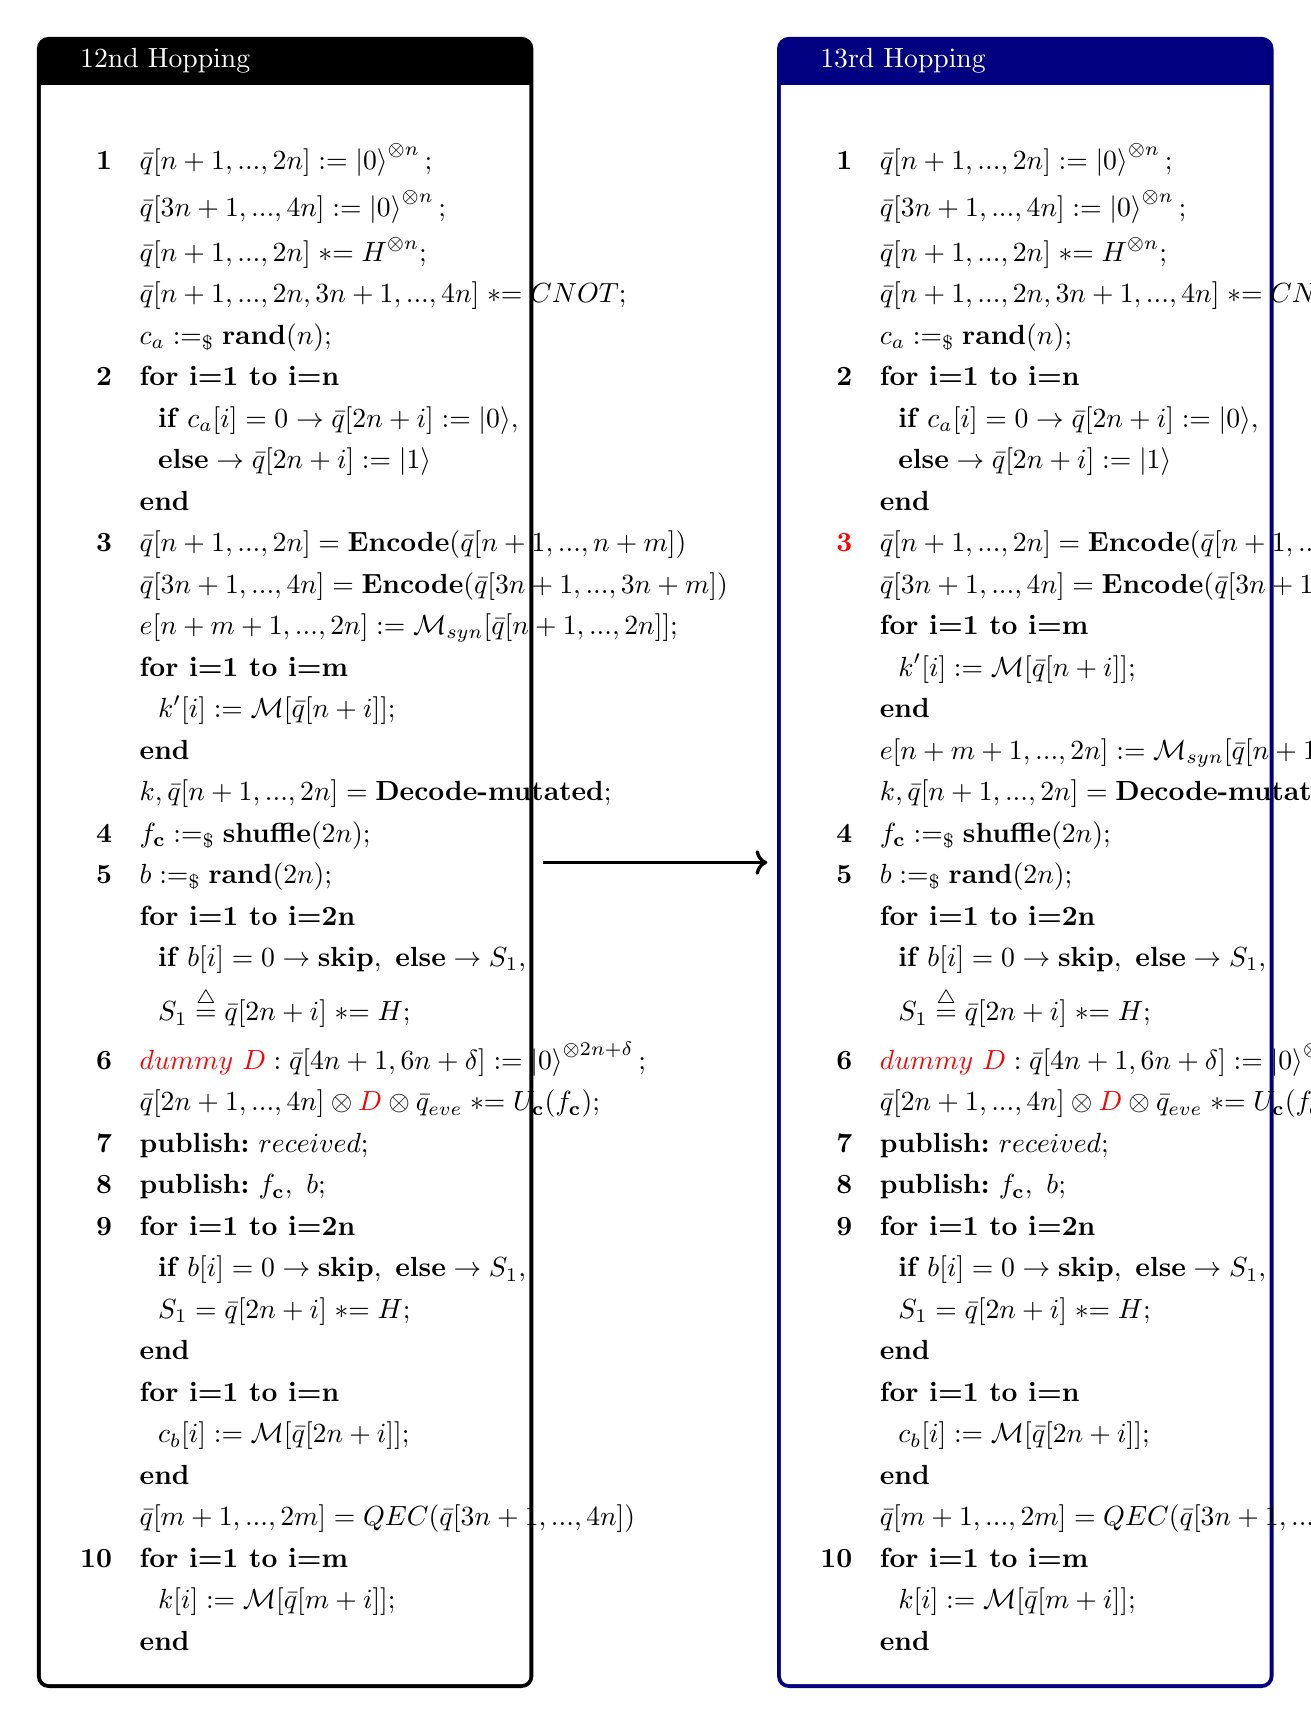
\begin{tikzpicture}[remember picture]

% Left box
\node[anchor=north west] (leftbox) at (0,0) {
\begin{minipage}[t]{0.52\textwidth}
\begin{tcolorbox}[colframe=black!75!black, colback=white, title=12nd Hopping, width=\textwidth]
\begin{align*}
    \textbf{{1}} \quad &\bar{q}[n+1,...,2n] := \ket{0}^{\otimes n};\\
    &\bar{q}[3n+1,...,4n] := \ket{0}^{\otimes n};\\
    \quad &\bar{q}[n+1,...,2n] \asteq H^{\otimes n}; \\
    &\bar{q}[n+1,...,2n,3n+1,...,4n] \asteq CNOT; \\
    & c_a :=_\$ \textbf{rand}(n); \\ 
    \textbf{{2}} \quad &\textbf{for i=1 to i=n}\\
    &~~ \textbf{if }  c_a[i] = 0 \rightarrow \bar{q}[2n+i] := |0\rangle,\\ &~~\textbf{else}   \rightarrow \bar{q}[2n+i] := |1\rangle\\
    &\textbf{end}\ \\
    \textbf{{3}} \quad &\bar{q}[n+1,...,2n]=\textbf{Encode}(\bar{q}[n+1,...,n+m])\\
    &\bar{q}[3n+1,...,4n]=\textbf{Encode}(\bar{q}[3n+1,...,3n+m])\\
    & e[n+m+1,...,2n]:=\mathcal{M}_{syn} [\bar{q}[n+1,...,2n]];\\
    & \textbf{for i=1 to i=m}\\
    &~~ k'[i]:= \mathcal{M} [\bar{q}[n+i]];\\
    &\textbf{end}\\
    \quad 
    & k,\bar{q}[n+1,...,2n]=\textbf{Decode-mutated};\\
    \textbf{{4}} \quad & f_{\textbf{c}}:=_\$\textbf{shuffle}(2n); \\
    \textbf{{5}} \quad & b :=_\$ \textbf{rand}(2n); \\
    &\textbf{for i=1 to i=2n}\\
    &~~ \textbf{if }  b[i] = 0 \rightarrow \textbf{skip},~\textbf{else}\rightarrow S_{1} ,\\
    &~~ S_{1}\stackrel{\triangle}{=}\bar{q}[2n+i] \asteq H ;\\
    \textbf{{6}} \quad & \textcolor{red}{dummy~D}: \bar{q}[4n+1,6n+\delta]:=\ket{0}^{\otimes 2n+\delta};\\     &\bar{q}[2n+1,...,4n]\otimes \textcolor{red}{D} \otimes \bar{q}_{eve} \asteq U_{\textbf{c}}(f_{\textbf{c}}); \\
    \textbf{{7}} \quad & \textbf{publish:}~ received;\\
    \textbf{{8}} \quad & \textbf{publish:}~ f_{\textbf{c}},~b;\\
    \textbf{{9}} \quad & \textbf{for i=1 to i=2n}\\
    &~~ \textbf{if }  b[i] = 0 \rightarrow \textbf{skip},~\textbf{else}\rightarrow S_{1} ,\\
    &~~ S_{1}=\bar{q}[2n+i] \asteq H ;\\
    &\textbf{end}\\
    \quad & \textbf{for~i=1~to~i=n}\\
    &~~ c_b[i]:= \mathcal{M} [\bar{q}[2n+i]];\\
    &\textbf{end}\\
    \quad & \bar{q}[m+1,...,2m]=QEC(\bar{q}[3n+1,...,4n])\\
    \textbf{{10}} \quad 
    & \textbf{for~i=1~to~i=m}\\
    &~~ k[i]:= \mathcal{M} [\bar{q}[m+i]];\\
    &\textbf{end}
\end{align*}
\end{tcolorbox}
\end{minipage}
};

% Right box
\node[anchor=north west] (rightbox) at (9.4,0) {
\begin{minipage}[t]{0.52\textwidth}
\begin{tcolorbox}[colframe=blue!50!black, colback=white, title=13rd Hopping, width=\textwidth]
\begin{align*}
    \textbf{{1}} \quad &\bar{q}[n+1,...,2n] := \ket{0}^{\otimes n};\\
    &\bar{q}[3n+1,...,4n] := \ket{0}^{\otimes n};\\
    \quad &\bar{q}[n+1,...,2n] \asteq H^{\otimes n}; \\
    &\bar{q}[n+1,...,2n,3n+1,...,4n] \asteq CNOT; \\
    & c_a :=_\$ \textbf{rand}(n); \\ 
    \textbf{{2}} \quad &\textbf{for i=1 to i=n}\\
    &~~ \textbf{if }  c_a[i] = 0 \rightarrow \bar{q}[2n+i] := |0\rangle,\\ &~~\textbf{else}   \rightarrow \bar{q}[2n+i] := |1\rangle\\
    &\textbf{end}\ \\
    \textbf{\textcolor{red}{3}} \quad &\bar{q}[n+1,...,2n]=\textbf{Encode}(\bar{q}[n+1,...,n+m])\\
    &\bar{q}[3n+1,...,4n]=\textbf{Encode}(\bar{q}[3n+1,...,3n+m])\\
    & \textbf{for i=1 to i=m}\\
    &~~ k'[i]:= \mathcal{M} [\bar{q}[n+i]];\\
    &\textbf{end}\\
    & e[n+m+1,...,2n]:=\mathcal{M}_{syn} [\bar{q}[n+1,...,2n]];\\
    & k,\bar{q}[n+1,...,2n]=\textbf{Decode-mutated};\\
    \textbf{{4}} \quad & f_{\textbf{c}}:=_\$\textbf{shuffle}(2n); \\
    \textbf{{5}} \quad & b :=_\$ \textbf{rand}(2n); \\
    &\textbf{for i=1 to i=2n}\\
    &~~ \textbf{if }  b[i] = 0 \rightarrow \textbf{skip},~\textbf{else}\rightarrow S_{1} ,\\
    &~~ S_{1}\stackrel{\triangle}{=}\bar{q}[2n+i] \asteq H ;\\
    \textbf{{6}} \quad & \textcolor{red}{dummy~D}: \bar{q}[4n+1,6n+\delta]:=\ket{0}^{\otimes 2n+\delta};\\     &\bar{q}[2n+1,...,4n]\otimes \textcolor{red}{D} \otimes \bar{q}_{eve} \asteq U_{\textbf{c}}(f_{\textbf{c}}); \\
    \textbf{{7}} \quad & \textbf{publish:}~ received;\\
    \textbf{{8}} \quad & \textbf{publish:}~ f_{\textbf{c}},~b;\\
    \textbf{{9}} \quad & \textbf{for i=1 to i=2n}\\
    &~~ \textbf{if }  b[i] = 0 \rightarrow \textbf{skip},~\textbf{else}\rightarrow S_{1} ,\\
    &~~ S_{1}=\bar{q}[2n+i] \asteq H ;\\
    &\textbf{end}\\
    \quad & \textbf{for~i=1~to~i=n}\\
    &~~ c_b[i]:= \mathcal{M} [\bar{q}[2n+i]];\\
    &\textbf{end}\\
    \quad & \bar{q}[m+1,...,2m]=QEC(\bar{q}[3n+1,...,4n])\\
    \textbf{{10}} \quad 
    & \textbf{for~i=1~to~i=m}\\
    &~~ k[i]:= \mathcal{M} [\bar{q}[m+i]];\\
    &\textbf{end}
\end{align*}
\end{tcolorbox}
\end{minipage}
};

% Draw arrow between boxes
\draw[->, very thick] (leftbox.east) -- node[above]{} (rightbox.west);

\end{tikzpicture}
\newpage

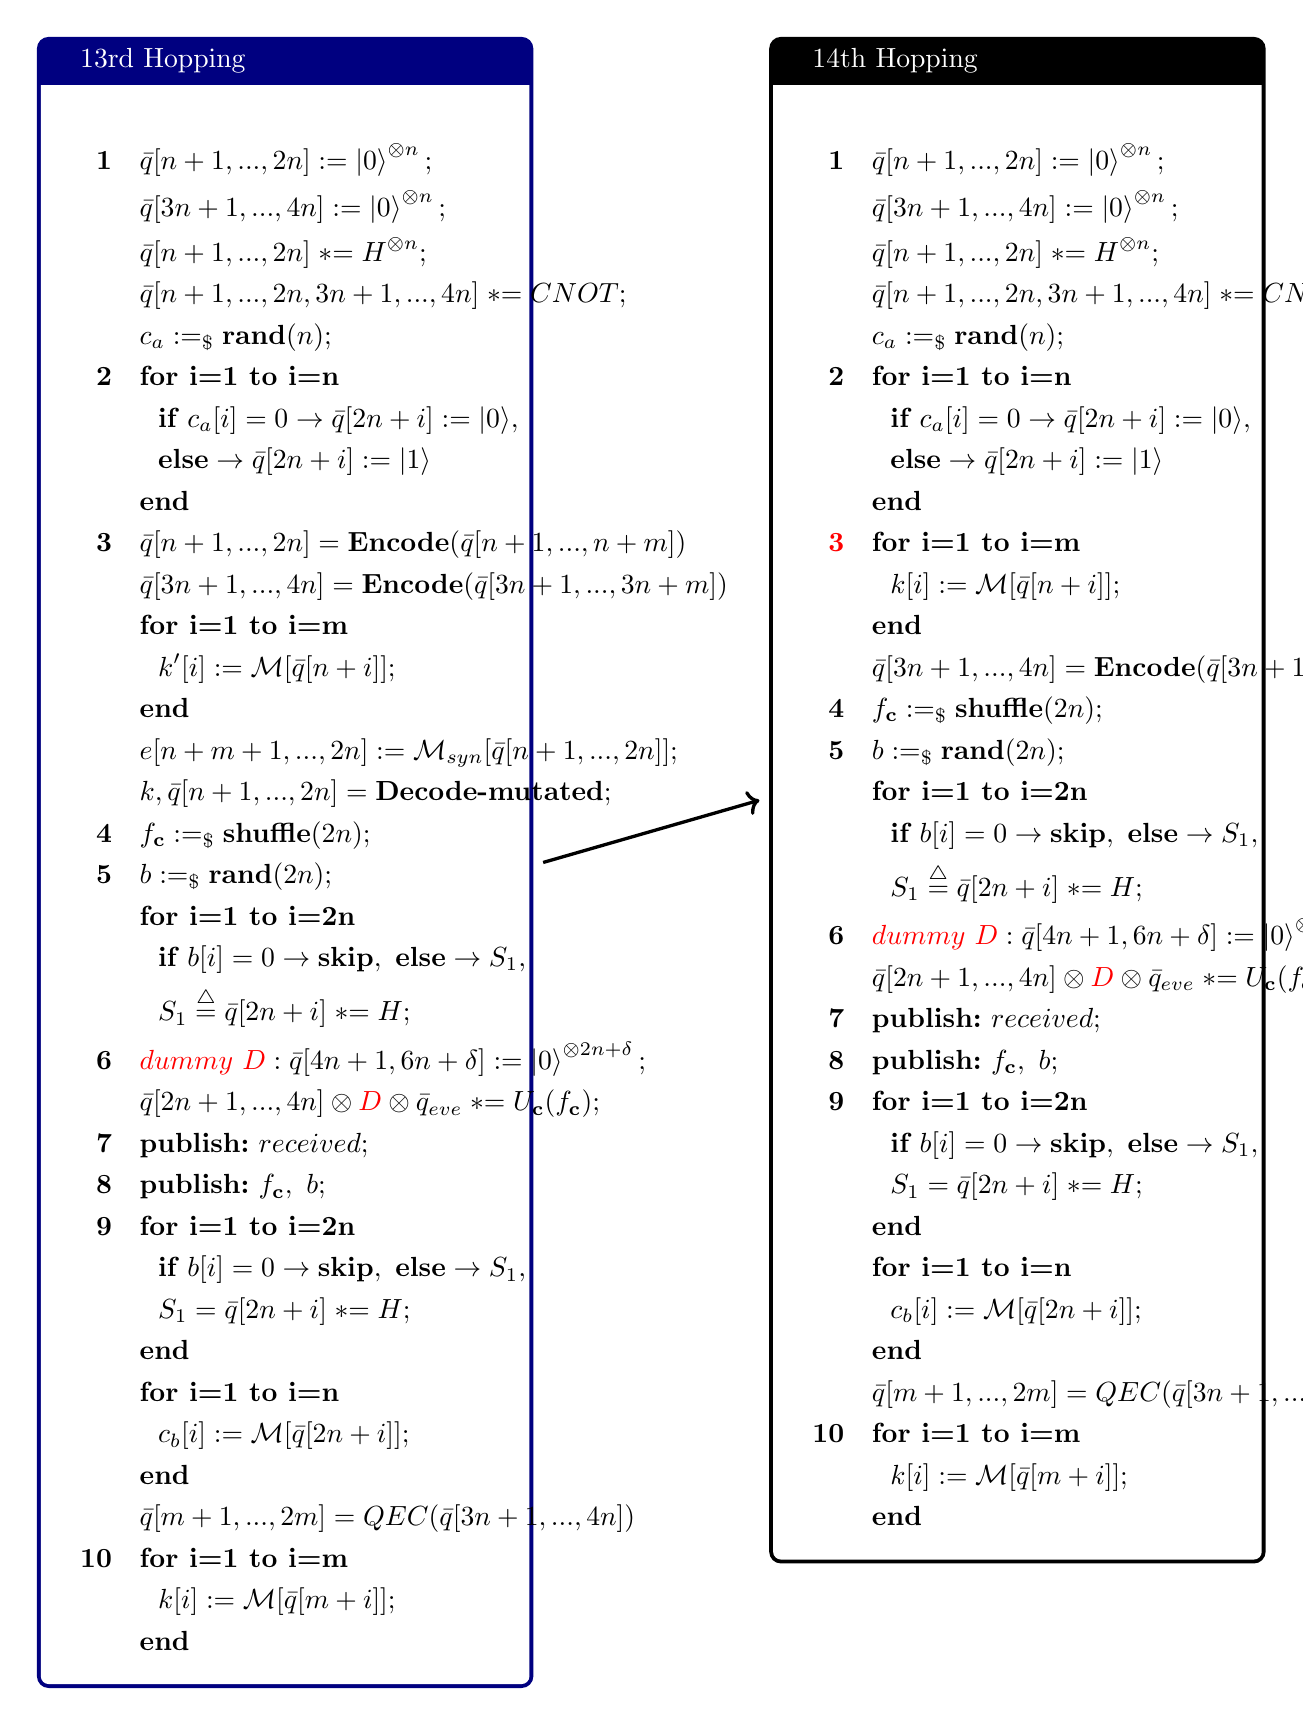
\begin{tikzpicture}[remember picture]

% Left box
\node[anchor=north west] (leftbox) at (0,0) {
\begin{minipage}[t]{0.52\textwidth}
\begin{tcolorbox}[colframe=blue!50!black, colback=white, title=13rd Hopping, width=\textwidth]
\begin{align*}
    \textbf{{1}} \quad &\bar{q}[n+1,...,2n] := \ket{0}^{\otimes n};\\
    &\bar{q}[3n+1,...,4n] := \ket{0}^{\otimes n};\\
    \quad &\bar{q}[n+1,...,2n] \asteq H^{\otimes n}; \\
    &\bar{q}[n+1,...,2n,3n+1,...,4n] \asteq CNOT; \\
    & c_a :=_\$ \textbf{rand}(n); \\ 
    \textbf{{2}} \quad &\textbf{for i=1 to i=n}\\
    &~~ \textbf{if }  c_a[i] = 0 \rightarrow \bar{q}[2n+i] := |0\rangle,\\ &~~\textbf{else}   \rightarrow \bar{q}[2n+i] := |1\rangle\\
    &\textbf{end}\ \\
    \textbf{{3}} \quad &\bar{q}[n+1,...,2n]=\textbf{Encode}(\bar{q}[n+1,...,n+m])\\
    &\bar{q}[3n+1,...,4n]=\textbf{Encode}(\bar{q}[3n+1,...,3n+m])\\
    & \textbf{for i=1 to i=m}\\
    &~~ k'[i]:= \mathcal{M} [\bar{q}[n+i]];\\
    &\textbf{end}\\
    & e[n+m+1,...,2n]:=\mathcal{M}_{syn} [\bar{q}[n+1,...,2n]];\\
    & k,\bar{q}[n+1,...,2n]=\textbf{Decode-mutated};\\
    \textbf{{4}} \quad & f_{\textbf{c}}:=_\$\textbf{shuffle}(2n); \\
    \textbf{{5}} \quad & b :=_\$ \textbf{rand}(2n); \\
    &\textbf{for i=1 to i=2n}\\
    &~~ \textbf{if }  b[i] = 0 \rightarrow \textbf{skip},~\textbf{else}\rightarrow S_{1} ,\\
    &~~ S_{1}\stackrel{\triangle}{=}\bar{q}[2n+i] \asteq H ;\\
    \textbf{{6}} \quad & \textcolor{red}{dummy~D}: \bar{q}[4n+1,6n+\delta]:=\ket{0}^{\otimes 2n+\delta};\\     &\bar{q}[2n+1,...,4n]\otimes \textcolor{red}{D} \otimes \bar{q}_{eve} \asteq U_{\textbf{c}}(f_{\textbf{c}}); \\
    \textbf{{7}} \quad & \textbf{publish:}~ received;\\
    \textbf{{8}} \quad & \textbf{publish:}~ f_{\textbf{c}},~b;\\
    \textbf{{9}} \quad & \textbf{for i=1 to i=2n}\\
    &~~ \textbf{if }  b[i] = 0 \rightarrow \textbf{skip},~\textbf{else}\rightarrow S_{1} ,\\
    &~~ S_{1}=\bar{q}[2n+i] \asteq H ;\\
    &\textbf{end}\\
    \quad & \textbf{for~i=1~to~i=n}\\
    &~~ c_b[i]:= \mathcal{M} [\bar{q}[2n+i]];\\
    &\textbf{end}\\
    \quad & \bar{q}[m+1,...,2m]=QEC(\bar{q}[3n+1,...,4n])\\
    \textbf{{10}} \quad 
    & \textbf{for~i=1~to~i=m}\\
    &~~ k[i]:= \mathcal{M} [\bar{q}[m+i]];\\
    &\textbf{end}
\end{align*}
\end{tcolorbox}
\end{minipage}
};

% Right box
\node[anchor=north west] (rightbox) at (9.3,0) {
\begin{minipage}[t]{0.52\textwidth}
\begin{tcolorbox}[colframe=black!50!black, colback=white, title=14th Hopping, width=\textwidth]
\begin{align*}
    \textbf{{1}} \quad &\bar{q}[n+1,...,2n] := \ket{0}^{\otimes n};\\
    &\bar{q}[3n+1,...,4n] := \ket{0}^{\otimes n};\\
    \quad &\bar{q}[n+1,...,2n] \asteq H^{\otimes n}; \\
    &\bar{q}[n+1,...,2n,3n+1,...,4n] \asteq CNOT; \\
    & c_a :=_\$ \textbf{rand}(n); \\ 
    \textbf{{2}} \quad &\textbf{for i=1 to i=n}\\
    &~~ \textbf{if }  c_a[i] = 0 \rightarrow \bar{q}[2n+i] := |0\rangle,\\ &~~\textbf{else}   \rightarrow \bar{q}[2n+i] := |1\rangle\\
    &\textbf{end}\ \\
    \textbf{\textcolor{red}{3}} \quad 
    & \textbf{for i=1 to i=m}\\
    &~~ k[i]:= \mathcal{M} [\bar{q}[n+i]];\\
    &\textbf{end}\\
    &\bar{q}[3n+1,...,4n]=\textbf{Encode}(\bar{q}[3n+1,...,3n+m])\\
    \textbf{{4}} \quad & f_{\textbf{c}}:=_\$\textbf{shuffle}(2n); \\
    \textbf{{5}} \quad & b :=_\$ \textbf{rand}(2n); \\
    &\textbf{for i=1 to i=2n}\\
    &~~ \textbf{if }  b[i] = 0 \rightarrow \textbf{skip},~\textbf{else}\rightarrow S_{1} ,\\
    &~~ S_{1}\stackrel{\triangle}{=}\bar{q}[2n+i] \asteq H ;\\
    \textbf{{6}} \quad & \textcolor{red}{dummy~D}: \bar{q}[4n+1,6n+\delta]:=\ket{0}^{\otimes 2n+\delta};\\     &\bar{q}[2n+1,...,4n]\otimes \textcolor{red}{D} \otimes \bar{q}_{eve} \asteq U_{\textbf{c}}(f_{\textbf{c}}); \\
    \textbf{{7}} \quad & \textbf{publish:}~ received;\\
    \textbf{{8}} \quad & \textbf{publish:}~ f_{\textbf{c}},~b;\\
    \textbf{{9}} \quad & \textbf{for i=1 to i=2n}\\
    &~~ \textbf{if }  b[i] = 0 \rightarrow \textbf{skip},~\textbf{else}\rightarrow S_{1} ,\\
    &~~ S_{1}=\bar{q}[2n+i] \asteq H ;\\
    &\textbf{end}\\
    \quad & \textbf{for~i=1~to~i=n}\\
    &~~ c_b[i]:= \mathcal{M} [\bar{q}[2n+i]];\\
    &\textbf{end}\\
    \quad & \bar{q}[m+1,...,2m]=QEC(\bar{q}[3n+1,...,4n])\\
    \textbf{{10}} \quad 
    & \textbf{for~i=1~to~i=m}\\
    &~~ k[i]:= \mathcal{M} [\bar{q}[m+i]];\\
    &\textbf{end}
\end{align*}
\end{tcolorbox}
\end{minipage}
};

% Draw arrow between boxes
\draw[->, very thick] (leftbox.east) -- node[above]{} (rightbox.west);

\end{tikzpicture}

$\textcolor{red}{QEC_{before-channel}(x)=QEC_{trival-error-correction}(x)}$
\newpage

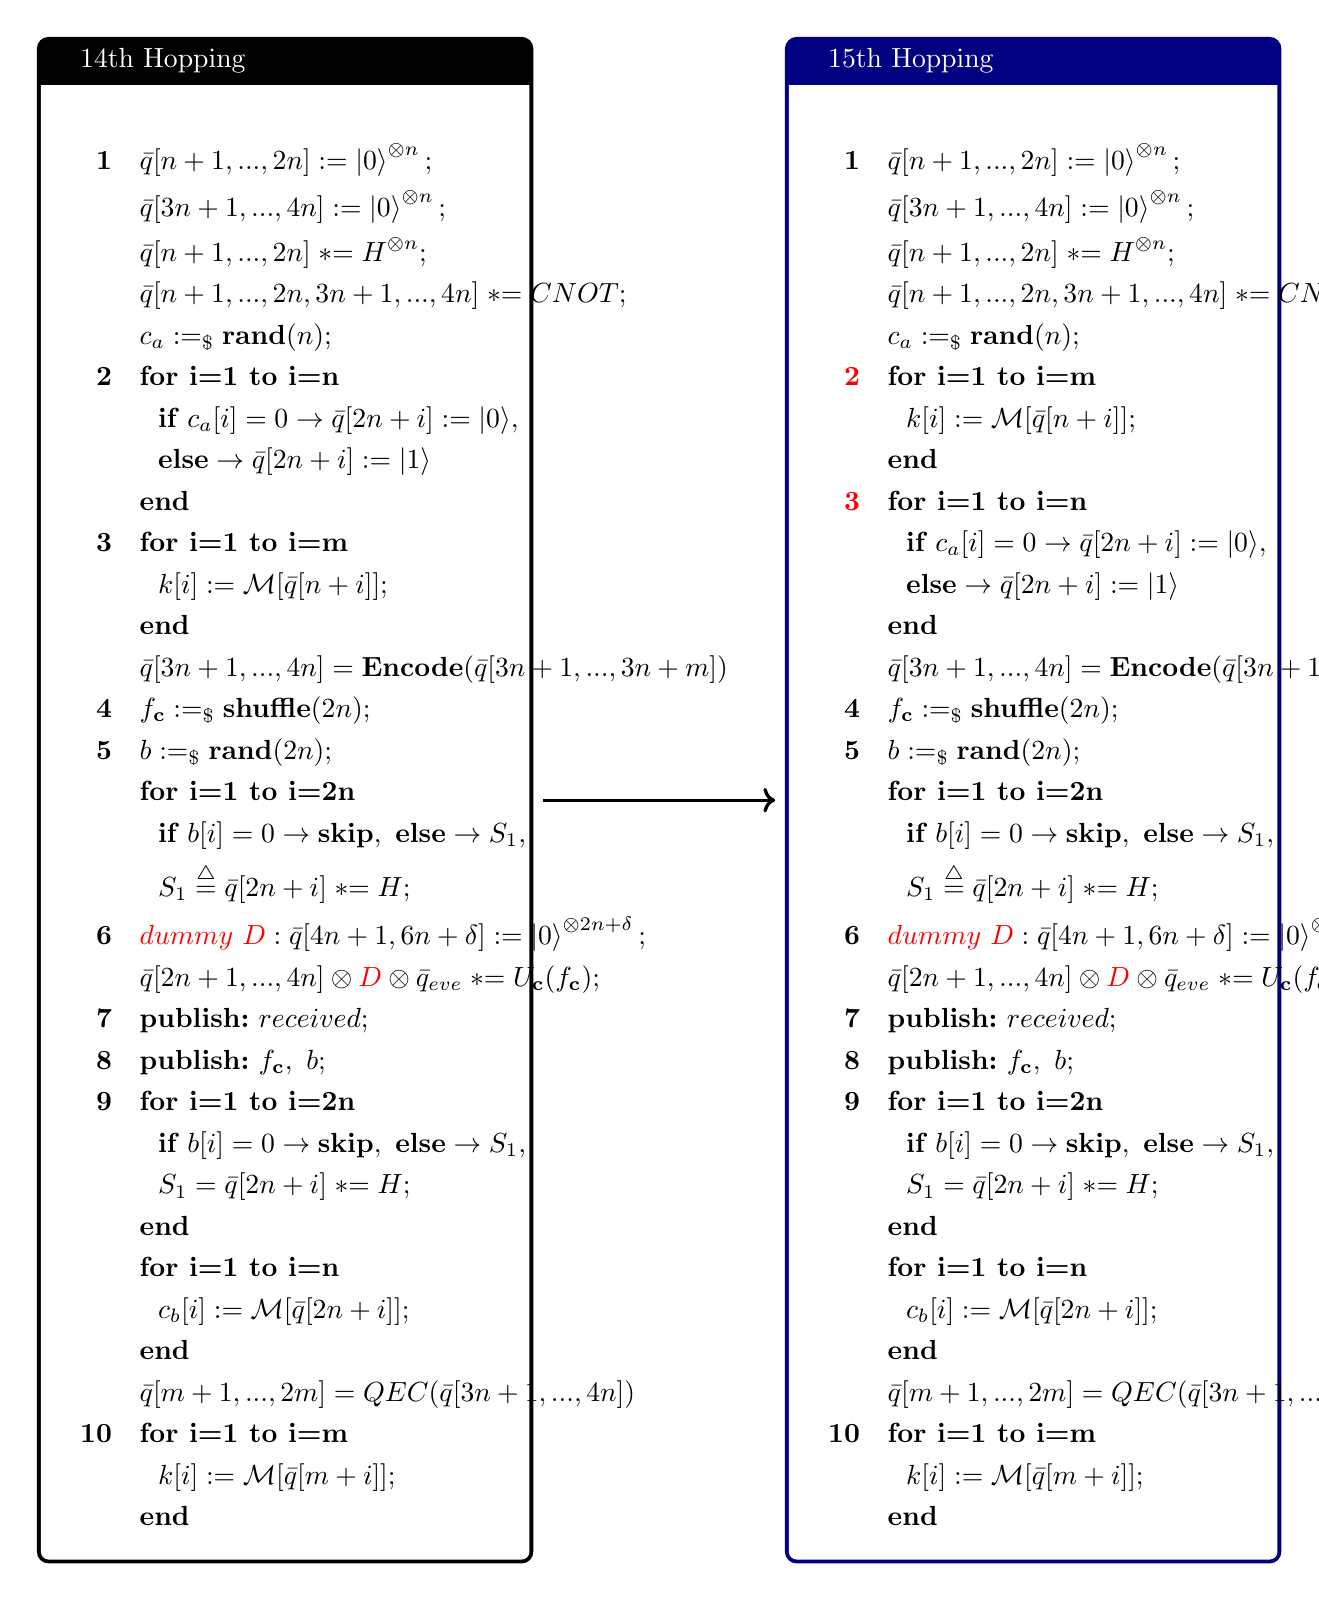
\begin{tikzpicture}[remember picture]

% Left box
\node[anchor=north west] (leftbox) at (0,0) {
\begin{minipage}[t]{0.52\textwidth}
\begin{tcolorbox}[colframe=black!75!black, colback=white, title=14th Hopping, width=\textwidth]
\begin{align*}
    \textbf{{1}} \quad &\bar{q}[n+1,...,2n] := \ket{0}^{\otimes n};\\
    &\bar{q}[3n+1,...,4n] := \ket{0}^{\otimes n};\\
    \quad &\bar{q}[n+1,...,2n] \asteq H^{\otimes n}; \\
    &\bar{q}[n+1,...,2n,3n+1,...,4n] \asteq CNOT; \\
    & c_a :=_\$ \textbf{rand}(n); \\ 
    \textbf{{2}} \quad &\textbf{for i=1 to i=n}\\
    &~~ \textbf{if }  c_a[i] = 0 \rightarrow \bar{q}[2n+i] := |0\rangle,\\ &~~\textbf{else}   \rightarrow \bar{q}[2n+i] := |1\rangle\\
    &\textbf{end}\ \\
    \textbf{{3}} \quad 
    & \textbf{for i=1 to i=m}\\
    &~~ k[i]:= \mathcal{M} [\bar{q}[n+i]];\\
    &\textbf{end}\\
    &\bar{q}[3n+1,...,4n]=\textbf{Encode}(\bar{q}[3n+1,...,3n+m])\\
    \textbf{{4}} \quad & f_{\textbf{c}}:=_\$\textbf{shuffle}(2n); \\
    \textbf{{5}} \quad & b :=_\$ \textbf{rand}(2n); \\
    &\textbf{for i=1 to i=2n}\\
    &~~ \textbf{if }  b[i] = 0 \rightarrow \textbf{skip},~\textbf{else}\rightarrow S_{1} ,\\
    &~~ S_{1}\stackrel{\triangle}{=}\bar{q}[2n+i] \asteq H ;\\
    \textbf{{6}} \quad & \textcolor{red}{dummy~D}: \bar{q}[4n+1,6n+\delta]:=\ket{0}^{\otimes 2n+\delta};\\     &\bar{q}[2n+1,...,4n]\otimes \textcolor{red}{D} \otimes \bar{q}_{eve} \asteq U_{\textbf{c}}(f_{\textbf{c}}); \\
    \textbf{{7}} \quad & \textbf{publish:}~ received;\\
    \textbf{{8}} \quad & \textbf{publish:}~ f_{\textbf{c}},~b;\\
    \textbf{{9}} \quad & \textbf{for i=1 to i=2n}\\
    &~~ \textbf{if }  b[i] = 0 \rightarrow \textbf{skip},~\textbf{else}\rightarrow S_{1} ,\\
    &~~ S_{1}=\bar{q}[2n+i] \asteq H ;\\
    &\textbf{end}\\
    \quad & \textbf{for~i=1~to~i=n}\\
    &~~ c_b[i]:= \mathcal{M} [\bar{q}[2n+i]];\\
    &\textbf{end}\\
    \quad & \bar{q}[m+1,...,2m]=QEC(\bar{q}[3n+1,...,4n])\\
    \textbf{{10}} \quad 
    & \textbf{for~i=1~to~i=m}\\
    &~~ k[i]:= \mathcal{M} [\bar{q}[m+i]];\\
    &\textbf{end}
\end{align*}
\end{tcolorbox}
\end{minipage}
};

% Right box
\node[anchor=north west] (rightbox) at (9.5,0) {
\begin{minipage}[t]{0.52\textwidth}
\begin{tcolorbox}[colframe=blue!50!black, colback=white, title=15th Hopping, width=\textwidth]
\begin{align*}
    \textbf{{1}} \quad &\bar{q}[n+1,...,2n] := \ket{0}^{\otimes n};\\
    &\bar{q}[3n+1,...,4n] := \ket{0}^{\otimes n};\\
    \quad &\bar{q}[n+1,...,2n] \asteq H^{\otimes n}; \\
    &\bar{q}[n+1,...,2n,3n+1,...,4n] \asteq CNOT; \\
    & c_a :=_\$ \textbf{rand}(n); \\ 
    \textbf{\textcolor{red}{2}} \quad 
    & \textbf{for i=1 to i=m}\\
    &~~ k[i]:= \mathcal{M} [\bar{q}[n+i]];\\
    &\textbf{end}\\
    \textbf{\textcolor{red}{3}} \quad 
    &\textbf{for i=1 to i=n}\\
    &~~ \textbf{if }  c_a[i] = 0 \rightarrow \bar{q}[2n+i] := |0\rangle,\\ &~~\textbf{else}   \rightarrow \bar{q}[2n+i] := |1\rangle\\
    &\textbf{end}\ \\
    &\bar{q}[3n+1,...,4n]=\textbf{Encode}(\bar{q}[3n+1,...,3n+m])\\ 
    \textbf{{4}} \quad & f_{\textbf{c}}:=_\$\textbf{shuffle}(2n); \\
    \textbf{{5}} \quad & b :=_\$ \textbf{rand}(2n); \\
    &\textbf{for i=1 to i=2n}\\
    &~~ \textbf{if }  b[i] = 0 \rightarrow \textbf{skip},~\textbf{else}\rightarrow S_{1} ,\\
    &~~ S_{1}\stackrel{\triangle}{=}\bar{q}[2n+i] \asteq H ;\\
    \textbf{{6}} \quad & \textcolor{red}{dummy~D}: \bar{q}[4n+1,6n+\delta]:=\ket{0}^{\otimes 2n+\delta};\\     &\bar{q}[2n+1,...,4n]\otimes \textcolor{red}{D} \otimes \bar{q}_{eve} \asteq U_{\textbf{c}}(f_{\textbf{c}}); \\
    \textbf{{7}} \quad & \textbf{publish:}~ received;\\
    \textbf{{8}} \quad & \textbf{publish:}~ f_{\textbf{c}},~b;\\
    \textbf{{9}} \quad & \textbf{for i=1 to i=2n}\\
    &~~ \textbf{if }  b[i] = 0 \rightarrow \textbf{skip},~\textbf{else}\rightarrow S_{1} ,\\
    &~~ S_{1}=\bar{q}[2n+i] \asteq H ;\\
    &\textbf{end}\\
    \quad & \textbf{for~i=1~to~i=n}\\
    &~~ c_b[i]:= \mathcal{M} [\bar{q}[2n+i]];\\
    &\textbf{end}\\
    \quad & \bar{q}[m+1,...,2m]=QEC(\bar{q}[3n+1,...,4n])\\
    \textbf{{10}} \quad 
    & \textbf{for~i=1~to~i=m}\\
    &~~ k[i]:= \mathcal{M} [\bar{q}[m+i]];\\
    &\textbf{end}
\end{align*}
\end{tcolorbox}
\end{minipage}
};

% Draw arrow between boxes
\draw[->, very thick] (leftbox.east) -- node[above]{} (rightbox.west);

\end{tikzpicture}
\newpage

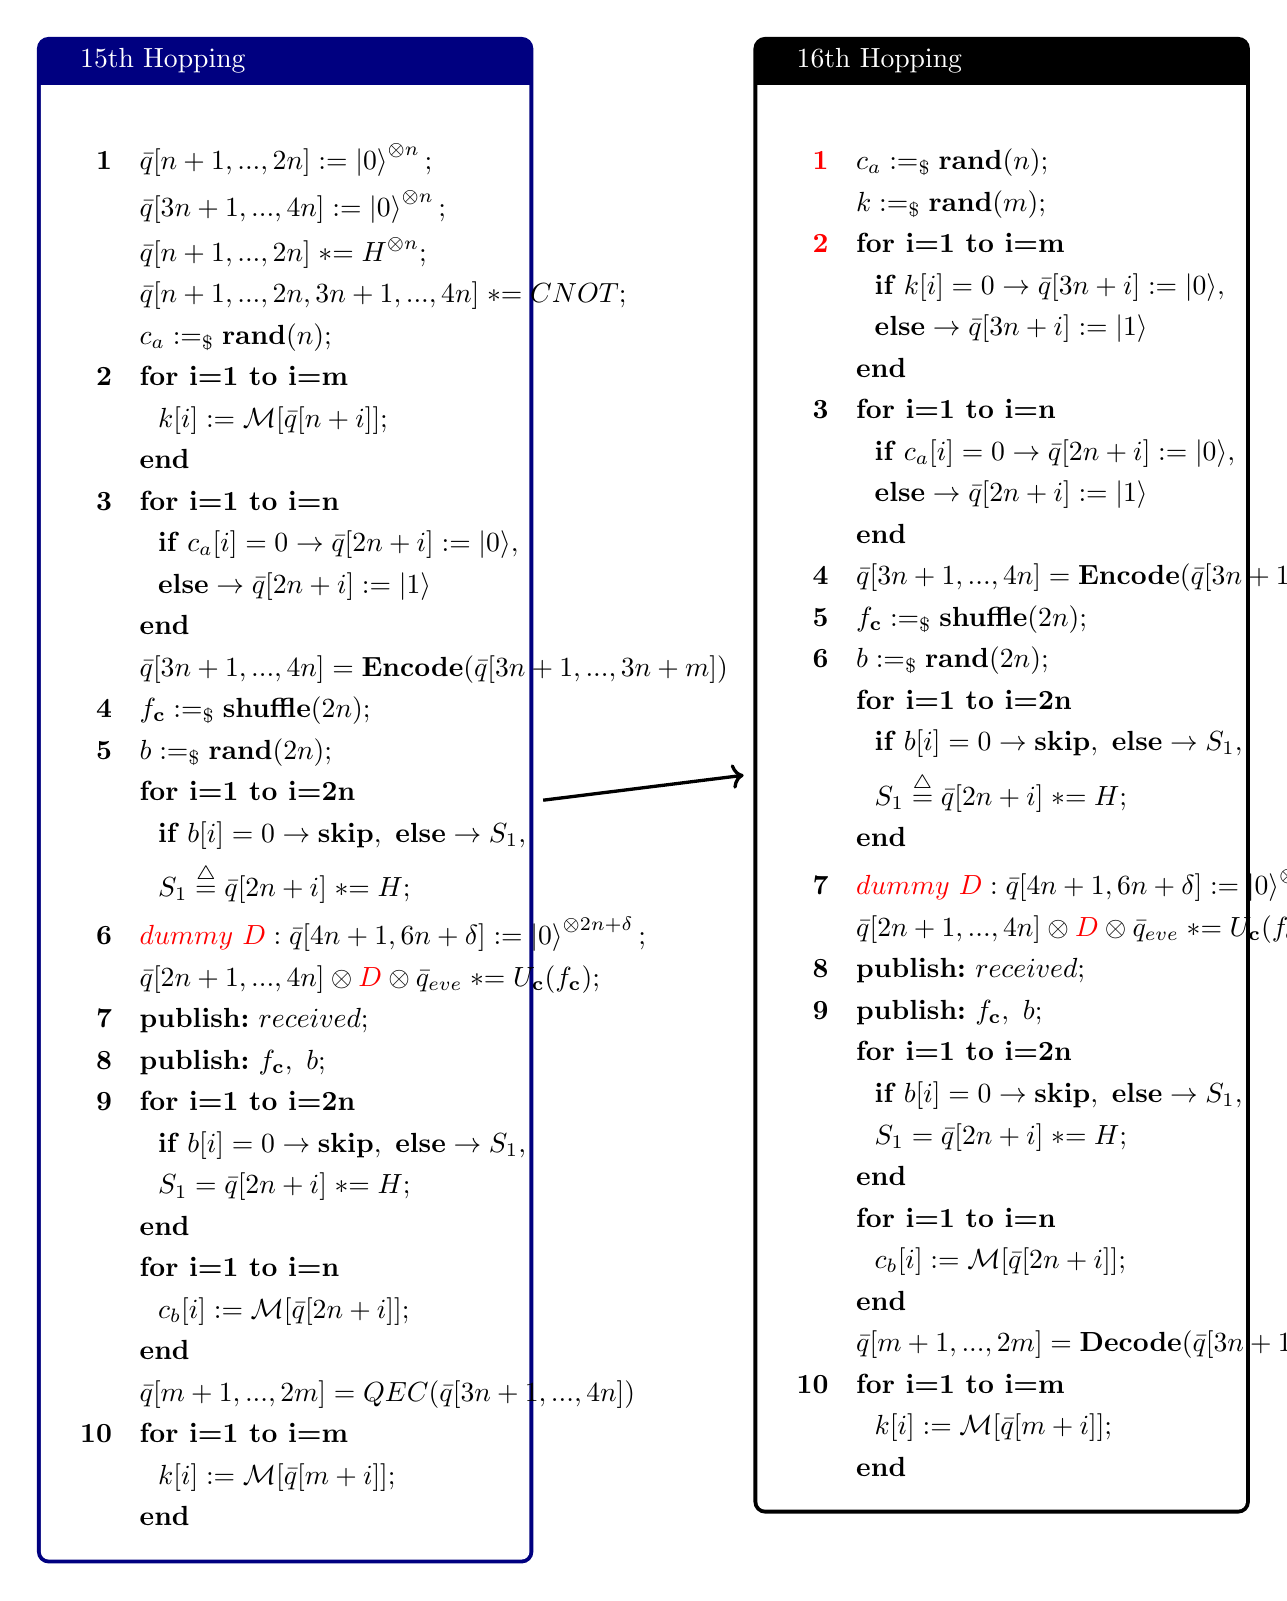
\begin{tikzpicture}[remember picture]

% Left box
\node[anchor=north west] (leftbox) at (0,0) {
\begin{minipage}[t]{0.52\textwidth}
\begin{tcolorbox}[colframe=blue!50!black, colback=white, title=15th Hopping, width=\textwidth]
\begin{align*}
    \textbf{{1}} \quad &\bar{q}[n+1,...,2n] := \ket{0}^{\otimes n};\\
    &\bar{q}[3n+1,...,4n] := \ket{0}^{\otimes n};\\
    \quad &\bar{q}[n+1,...,2n] \asteq H^{\otimes n}; \\
    &\bar{q}[n+1,...,2n,3n+1,...,4n] \asteq CNOT; \\
    & c_a :=_\$ \textbf{rand}(n); \\ 
    \textbf{{2}} \quad 
    & \textbf{for i=1 to i=m}\\
    &~~ k[i]:= \mathcal{M} [\bar{q}[n+i]];\\
    &\textbf{end}\\
    \textbf{{3}} \quad 
    &\textbf{for i=1 to i=n}\\
    &~~ \textbf{if }  c_a[i] = 0 \rightarrow \bar{q}[2n+i] := |0\rangle,\\ &~~\textbf{else}   \rightarrow \bar{q}[2n+i] := |1\rangle\\
    &\textbf{end}\ \\
    &\bar{q}[3n+1,...,4n]=\textbf{Encode}(\bar{q}[3n+1,...,3n+m])\\ 
    \textbf{{4}} \quad & f_{\textbf{c}}:=_\$\textbf{shuffle}(2n); \\
    \textbf{{5}} \quad & b :=_\$ \textbf{rand}(2n); \\
    &\textbf{for i=1 to i=2n}\\
    &~~ \textbf{if }  b[i] = 0 \rightarrow \textbf{skip},~\textbf{else}\rightarrow S_{1} ,\\
    &~~ S_{1}\stackrel{\triangle}{=}\bar{q}[2n+i] \asteq H ;\\
    \textbf{{6}} \quad & \textcolor{red}{dummy~D}: \bar{q}[4n+1,6n+\delta]:=\ket{0}^{\otimes 2n+\delta};\\     &\bar{q}[2n+1,...,4n]\otimes \textcolor{red}{D} \otimes \bar{q}_{eve} \asteq U_{\textbf{c}}(f_{\textbf{c}}); \\
    \textbf{{7}} \quad & \textbf{publish:}~ received;\\
    \textbf{{8}} \quad & \textbf{publish:}~ f_{\textbf{c}},~b;\\
    \textbf{{9}} \quad & \textbf{for i=1 to i=2n}\\
    &~~ \textbf{if }  b[i] = 0 \rightarrow \textbf{skip},~\textbf{else}\rightarrow S_{1} ,\\
    &~~ S_{1}=\bar{q}[2n+i] \asteq H ;\\
    &\textbf{end}\\
    \quad & \textbf{for~i=1~to~i=n}\\
    &~~ c_b[i]:= \mathcal{M} [\bar{q}[2n+i]];\\
    &\textbf{end}\\
    \quad & \bar{q}[m+1,...,2m]=QEC(\bar{q}[3n+1,...,4n])\\
    \textbf{{10}} \quad 
    & \textbf{for~i=1~to~i=m}\\
    &~~ k[i]:= \mathcal{M} [\bar{q}[m+i]];\\
    &\textbf{end}
\end{align*}
\end{tcolorbox}
\end{minipage}
};

% Right box
\node[anchor=north west] (rightbox) at (9.1,0) {
\begin{minipage}[t]{0.52\textwidth}
\begin{tcolorbox}[colframe=black!50!black, colback=white, title=16th Hopping, width=\textwidth]
\begin{align*}
    \textbf{\textcolor{red}{1}} \quad 
    & c_a :=_\$ \textbf{rand}(n); \\ 
    & k :=_\$ \textbf{rand}(m); \\  \textbf{\textcolor{red}{2}} \quad &\textbf{for i=1 to i=m}\\
    &~~ \textbf{if }  k[i] = 0 \rightarrow \bar{q}[3n+i] := |0\rangle,\\ &~~\textbf{else}   \rightarrow \bar{q}[3n+i] := |1\rangle\\
    &\textbf{end}\ \\
    \textbf{{3}} \quad 
    &\textbf{for i=1 to i=n}\\
    &~~ \textbf{if }  c_a[i] = 0 \rightarrow \bar{q}[2n+i] := |0\rangle,\\ &~~\textbf{else}   \rightarrow \bar{q}[2n+i] := |1\rangle\\
    &\textbf{end}\ \\
    \textbf{{4}} \quad 
    &\bar{q}[3n+1,...,4n]=\textbf{Encode}(\bar{q}[3n+1,...,3n+m])\\
    \textbf{{5}} \quad & f_{\textbf{c}}:=_\$\textbf{shuffle}(2n); \\
    \textbf{{6}} \quad & b :=_\$ \textbf{rand}(2n); \\
    &\textbf{for i=1 to i=2n}\\
    &~~ \textbf{if }  b[i] = 0 \rightarrow \textbf{skip},~\textbf{else}\rightarrow S_{1} ,\\
    &~~ S_{1}\stackrel{\triangle}{=}\bar{q}[2n+i] \asteq H ;\\
    &\textbf{end}\\
    \textbf{{7}} \quad & \textcolor{red}{dummy~D}: \bar{q}[4n+1,6n+\delta]:=\ket{0}^{\otimes 2n+\delta};\\     &\bar{q}[2n+1,...,4n]\otimes \textcolor{red}{D} \otimes \bar{q}_{eve} \asteq U_{\textbf{c}}(f_{\textbf{c}}); \\
    \textbf{{8}} \quad & \textbf{publish:}~ received;\\
    \textbf{{9}} \quad & \textbf{publish:}~ f_{\textbf{c}},~b;\\
    \quad & \textbf{for i=1 to i=2n}\\
    &~~ \textbf{if }  b[i] = 0 \rightarrow \textbf{skip},~\textbf{else}\rightarrow S_{1} ,\\
    &~~ S_{1}=\bar{q}[2n+i] \asteq H ;\\
    &\textbf{end}\\
    \quad & \textbf{for~i=1~to~i=n}\\
    &~~ c_b[i]:= \mathcal{M} [\bar{q}[2n+i]];\\
    &\textbf{end}\\
    \quad & \bar{q}[m+1,...,2m]=\textbf{Decode}(\bar{q}[3n+1,...,4n])\\
    \textbf{{10}} \quad 
    & \textbf{for~i=1~to~i=m}\\
    &~~ k[i]:= \mathcal{M} [\bar{q}[m+i]];\\
    &\textbf{end}
\end{align*}
\end{tcolorbox}
\end{minipage}
};

% Draw arrow between boxes
\draw[->, very thick] (leftbox.east) -- node[above]{} (rightbox.west);

\end{tikzpicture}
\newpage

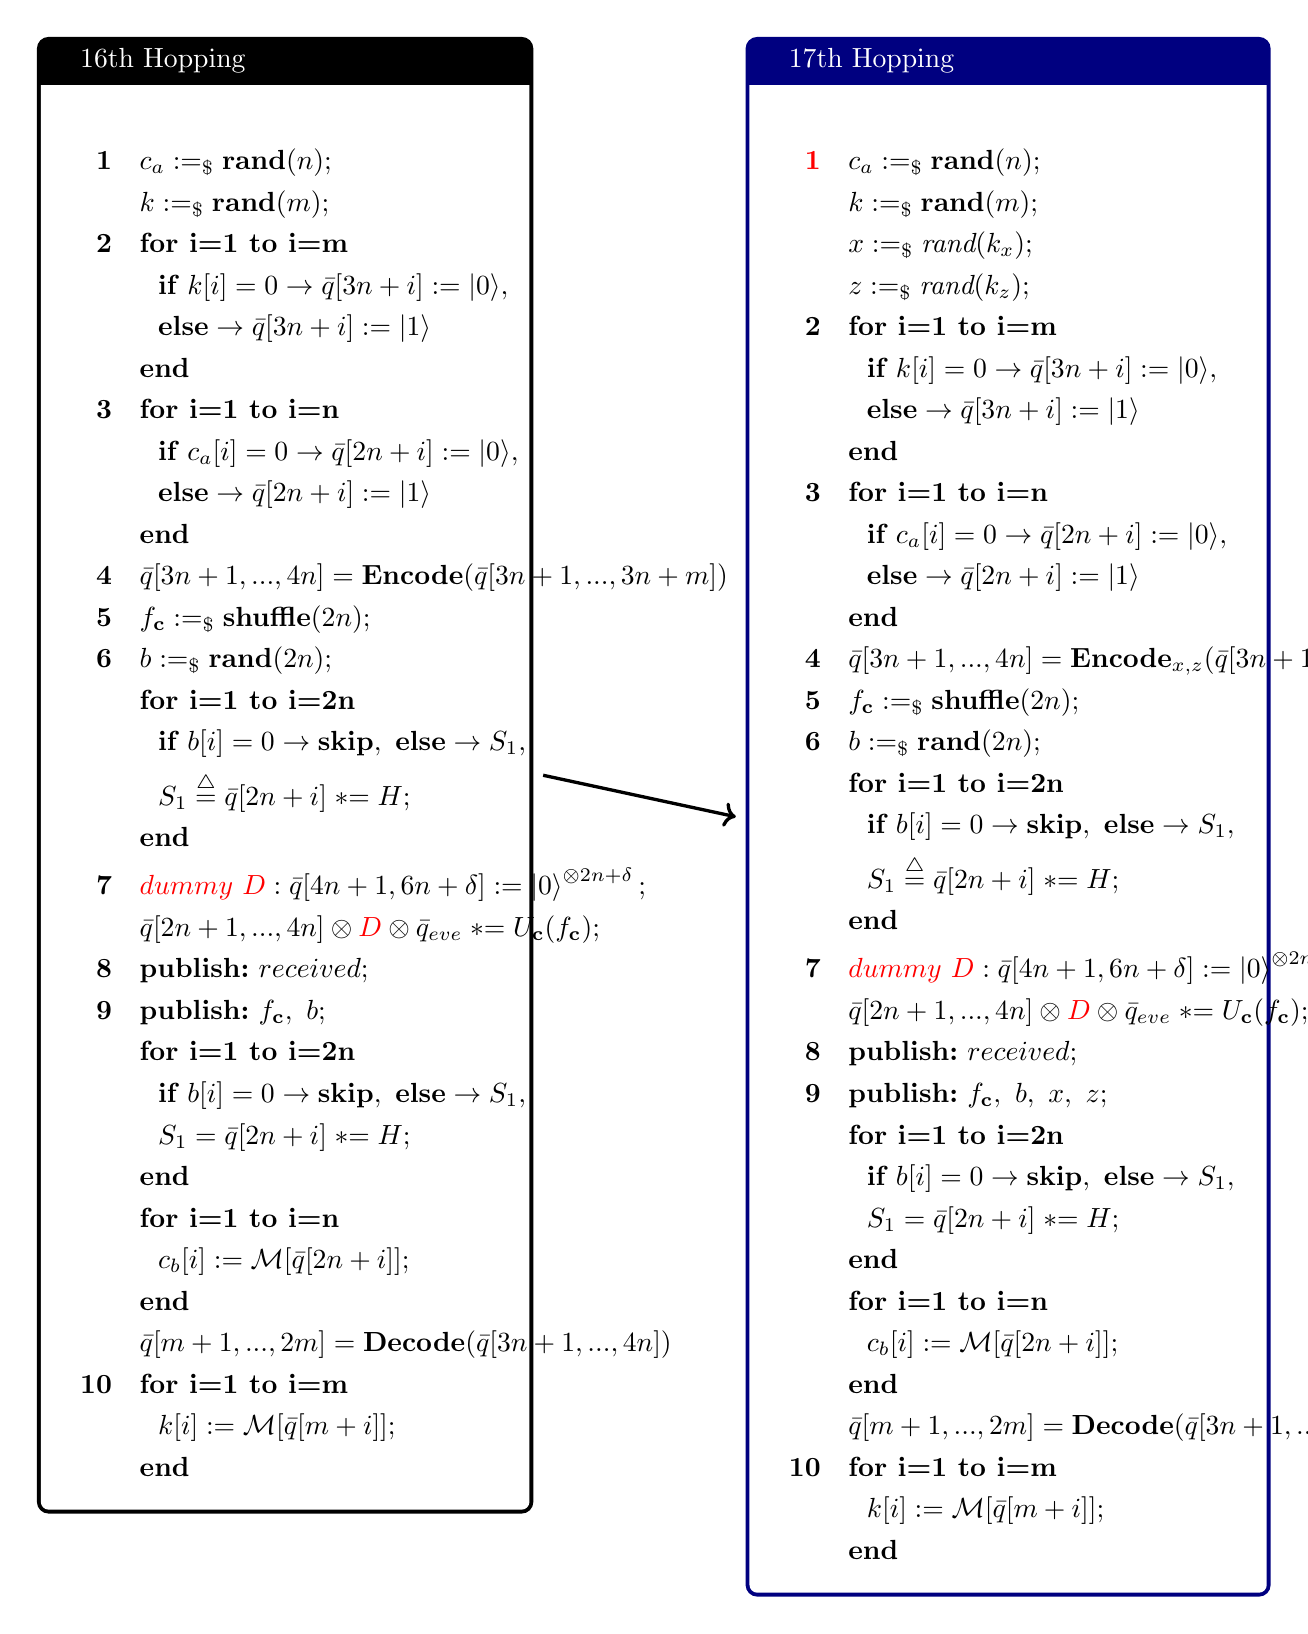
\begin{tikzpicture}[remember picture]

% Left box
\node[anchor=north west] (leftbox) at (0,0) {
\begin{minipage}[t]{0.52\textwidth}
\begin{tcolorbox}[colframe=black!50!black, colback=white, title=16th Hopping, width=\textwidth]
\begin{align*}
    \textbf{{1}} \quad 
    & c_a :=_\$ \textbf{rand}(n); \\ 
    & k :=_\$ \textbf{rand}(m); \\  \textbf{{2}} \quad &\textbf{for i=1 to i=m}\\
    &~~ \textbf{if }  k[i] = 0 \rightarrow \bar{q}[3n+i] := |0\rangle,\\ &~~\textbf{else}   \rightarrow \bar{q}[3n+i] := |1\rangle\\
    &\textbf{end}\ \\
    \textbf{{3}} \quad 
    &\textbf{for i=1 to i=n}\\
    &~~ \textbf{if }  c_a[i] = 0 \rightarrow \bar{q}[2n+i] := |0\rangle,\\ &~~\textbf{else}   \rightarrow \bar{q}[2n+i] := |1\rangle\\
    &\textbf{end}\ \\
    \textbf{{4}} \quad 
    &\bar{q}[3n+1,...,4n]=\textbf{Encode}(\bar{q}[3n+1,...,3n+m])\\
    \textbf{{5}} \quad & f_{\textbf{c}}:=_\$\textbf{shuffle}(2n); \\
    \textbf{{6}} \quad & b :=_\$ \textbf{rand}(2n); \\
    &\textbf{for i=1 to i=2n}\\
    &~~ \textbf{if }  b[i] = 0 \rightarrow \textbf{skip},~\textbf{else}\rightarrow S_{1} ,\\
    &~~ S_{1}\stackrel{\triangle}{=}\bar{q}[2n+i] \asteq H ;\\
    &\textbf{end}\\
    \textbf{{7}} \quad & \textcolor{red}{dummy~D}: \bar{q}[4n+1,6n+\delta]:=\ket{0}^{\otimes 2n+\delta};\\     &\bar{q}[2n+1,...,4n]\otimes \textcolor{red}{D} \otimes \bar{q}_{eve} \asteq U_{\textbf{c}}(f_{\textbf{c}}); \\
    \textbf{{8}} \quad & \textbf{publish:}~ received;\\
    \textbf{{9}} \quad & \textbf{publish:}~ f_{\textbf{c}},~b;\\
    \quad & \textbf{for i=1 to i=2n}\\
    &~~ \textbf{if }  b[i] = 0 \rightarrow \textbf{skip},~\textbf{else}\rightarrow S_{1} ,\\
    &~~ S_{1}=\bar{q}[2n+i] \asteq H ;\\
    &\textbf{end}\\
    \quad & \textbf{for~i=1~to~i=n}\\
    &~~ c_b[i]:= \mathcal{M} [\bar{q}[2n+i]];\\
    &\textbf{end}\\
    \quad & \bar{q}[m+1,...,2m]=\textbf{Decode}(\bar{q}[3n+1,...,4n])\\
    \textbf{{10}} \quad 
    & \textbf{for~i=1~to~i=m}\\
    &~~ k[i]:= \mathcal{M} [\bar{q}[m+i]];\\
    &\textbf{end}
\end{align*}
\end{tcolorbox}
\end{minipage}
};

% Right box
\node[anchor=north west] (rightbox) at (9,0) {
\begin{minipage}[t]{0.55\textwidth}
\begin{tcolorbox}[colframe=blue!50!black, colback=white, title=17th Hopping, width=\textwidth]
\begin{align*}
    \textbf{\textcolor{red}{1}} \quad 
    & c_a :=_\$ \textbf{rand}(n); \\ 
    & k :=_\$ \textbf{rand}(m); \\ 
    & x :=_\$ \textit{rand}(k_x); \\
    & z :=_\$ \textit{rand}(k_z); \\ \textbf{{2}} \quad &\textbf{for i=1 to i=m}\\
    &~~ \textbf{if }  k[i] = 0 \rightarrow \bar{q}[3n+i] := |0\rangle,\\ &~~\textbf{else}   \rightarrow \bar{q}[3n+i] := |1\rangle\\
    &\textbf{end}\ \\
    \textbf{{3}} \quad 
    &\textbf{for i=1 to i=n}\\
    &~~ \textbf{if }  c_a[i] = 0 \rightarrow \bar{q}[2n+i] := |0\rangle,\\ &~~\textbf{else}   \rightarrow \bar{q}[2n+i] := |1\rangle\\
    &\textbf{end}\ \\
    \textbf{{4}} \quad 
    &\bar{q}[3n+1,...,4n]=\textbf{Encode}_{x,z}(\bar{q}[3n+1,...,3n+m])\\
    \textbf{{5}} \quad & f_{\textbf{c}}:=_\$\textbf{shuffle}(2n); \\
    \textbf{{6}} \quad & b :=_\$ \textbf{rand}(2n); \\
    &\textbf{for i=1 to i=2n}\\
    &~~ \textbf{if }  b[i] = 0 \rightarrow \textbf{skip},~\textbf{else}\rightarrow S_{1} ,\\
    &~~ S_{1}\stackrel{\triangle}{=}\bar{q}[2n+i] \asteq H ;\\
    &\textbf{end}\\
    \textbf{{7}} \quad & \textcolor{red}{dummy~D}: \bar{q}[4n+1,6n+\delta]:=\ket{0}^{\otimes 2n+\delta};\\     &\bar{q}[2n+1,...,4n]\otimes \textcolor{red}{D} \otimes \bar{q}_{eve} \asteq U_{\textbf{c}}(f_{\textbf{c}}); \\
    \textbf{{8}} \quad & \textbf{publish:}~ received;\\
    \textbf{{9}} \quad & \textbf{publish:}~ f_{\textbf{c}},~b, ~x,~ z;\\
    \quad & \textbf{for i=1 to i=2n}\\
    &~~ \textbf{if }  b[i] = 0 \rightarrow \textbf{skip},~\textbf{else}\rightarrow S_{1} ,\\
    &~~ S_{1}=\bar{q}[2n+i] \asteq H ;\\
    &\textbf{end}\\
    \quad & \textbf{for~i=1~to~i=n}\\
    &~~ c_b[i]:= \mathcal{M} [\bar{q}[2n+i]];\\
    &\textbf{end}\\
    \quad & \bar{q}[m+1,...,2m]=\textbf{Decode}(\bar{q}[3n+1,...,4n])\\
    \textbf{{10}} \quad 
    & \textbf{for~i=1~to~i=m}\\
    &~~ k[i]:= \mathcal{M} [\bar{q}[m+i]];\\
    &\textbf{end}
\end{align*}
\end{tcolorbox}
\end{minipage}
};

% Draw arrow between boxes
\draw[->, very thick] (leftbox.east) -- node[above]{} (rightbox.west);

\end{tikzpicture}
\newpage

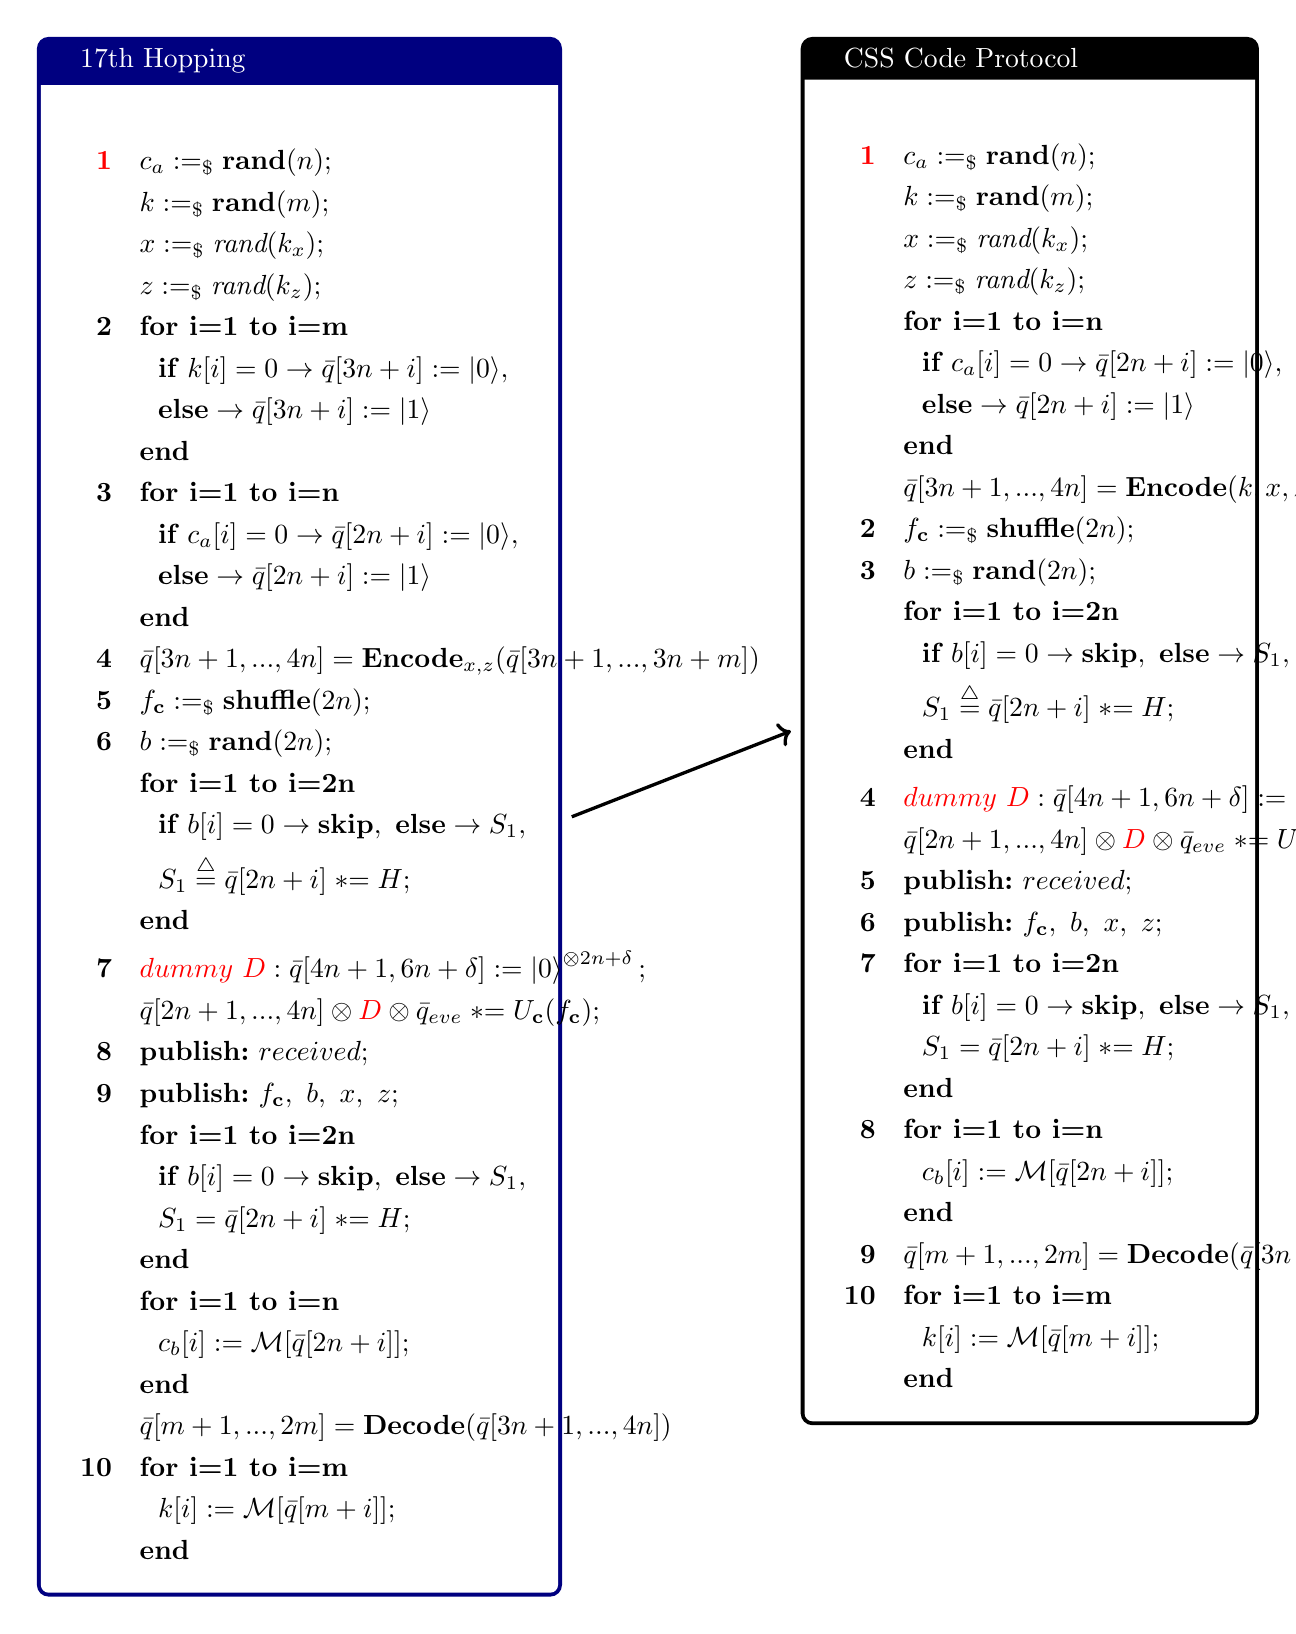
\begin{tikzpicture}[remember picture]

% Left box
\node[anchor=north west] (leftbox) at (0,0) {
\begin{minipage}[t]{0.55\textwidth}
\begin{tcolorbox}[colframe=blue!50!black, colback=white, title=17th Hopping, width=\textwidth]
\begin{align*}
    \textbf{\textcolor{red}{1}} \quad 
    & c_a :=_\$ \textbf{rand}(n); \\ 
    & k :=_\$ \textbf{rand}(m); \\ 
    & x :=_\$ \textit{rand}(k_x); \\
    & z :=_\$ \textit{rand}(k_z); \\ \textbf{{2}} \quad &\textbf{for i=1 to i=m}\\
    &~~ \textbf{if }  k[i] = 0 \rightarrow \bar{q}[3n+i] := |0\rangle,\\ &~~\textbf{else}   \rightarrow \bar{q}[3n+i] := |1\rangle\\
    &\textbf{end}\ \\
    \textbf{{3}} \quad 
    &\textbf{for i=1 to i=n}\\
    &~~ \textbf{if }  c_a[i] = 0 \rightarrow \bar{q}[2n+i] := |0\rangle,\\ &~~\textbf{else}   \rightarrow \bar{q}[2n+i] := |1\rangle\\
    &\textbf{end}\ \\
    \textbf{{4}} \quad 
    &\bar{q}[3n+1,...,4n]=\textbf{Encode}_{x,z}(\bar{q}[3n+1,...,3n+m])\\
    \textbf{{5}} \quad & f_{\textbf{c}}:=_\$\textbf{shuffle}(2n); \\
    \textbf{{6}} \quad & b :=_\$ \textbf{rand}(2n); \\
    &\textbf{for i=1 to i=2n}\\
    &~~ \textbf{if }  b[i] = 0 \rightarrow \textbf{skip},~\textbf{else}\rightarrow S_{1} ,\\
    &~~ S_{1}\stackrel{\triangle}{=}\bar{q}[2n+i] \asteq H ;\\
    &\textbf{end}\\
    \textbf{{7}} \quad & \textcolor{red}{dummy~D}: \bar{q}[4n+1,6n+\delta]:=\ket{0}^{\otimes 2n+\delta};\\     &\bar{q}[2n+1,...,4n]\otimes \textcolor{red}{D} \otimes \bar{q}_{eve} \asteq U_{\textbf{c}}(f_{\textbf{c}}); \\
    \textbf{{8}} \quad & \textbf{publish:}~ received;\\
    \textbf{{9}} \quad & \textbf{publish:}~ f_{\textbf{c}},~b, ~x,~ z;\\
    \quad & \textbf{for i=1 to i=2n}\\
    &~~ \textbf{if }  b[i] = 0 \rightarrow \textbf{skip},~\textbf{else}\rightarrow S_{1} ,\\
    &~~ S_{1}=\bar{q}[2n+i] \asteq H ;\\
    &\textbf{end}\\
    \quad & \textbf{for~i=1~to~i=n}\\
    &~~ c_b[i]:= \mathcal{M} [\bar{q}[2n+i]];\\
    &\textbf{end}\\
    \quad & \bar{q}[m+1,...,2m]=\textbf{Decode}(\bar{q}[3n+1,...,4n])\\
    \textbf{{10}} \quad 
    & \textbf{for~i=1~to~i=m}\\
    &~~ k[i]:= \mathcal{M} [\bar{q}[m+i]];\\
    &\textbf{end}
\end{align*}
\end{tcolorbox}
\end{minipage}
};

% Right box
\node[anchor=north west] (rightbox) at (9.7,0) {
\begin{minipage}[t]{0.48\textwidth}
\begin{tcolorbox}[colframe=black!50!black, colback=white, title=CSS Code Protocol, width=\textwidth]
\begin{align*}
    \textbf{\textcolor{red}{1}} \quad 
    & c_a :=_\$ \textbf{rand}(n); \\ 
    & k :=_\$ \textbf{rand}(m); \\ 
    & x :=_\$ \textit{rand}(k_x); \\
    & z :=_\$ \textit{rand}(k_z); \\
    \quad 
    &\textbf{for i=1 to i=n}\\
    &~~ \textbf{if }  c_a[i] = 0 \rightarrow \bar{q}[2n+i] := |0\rangle,\\ &~~\textbf{else}   \rightarrow \bar{q}[2n+i] := |1\rangle\\
    &\textbf{end}\ \\
    \quad 
    &\bar{q}[3n+1,...,4n]=\textbf{Encode}(k,x,z)\\
    \textbf{{2}} \quad & f_{\textbf{c}}:=_\$\textbf{shuffle}(2n); \\
    \textbf{{3}} \quad & b :=_\$ \textbf{rand}(2n); \\
    &\textbf{for i=1 to i=2n}\\
    &~~ \textbf{if }  b[i] = 0 \rightarrow \textbf{skip},~\textbf{else}\rightarrow S_{1} ,\\
    &~~ S_{1}\stackrel{\triangle}{=}\bar{q}[2n+i] \asteq H ;\\
    &\textbf{end}\\
    \textbf{{4}} \quad & \textcolor{red}{dummy~D}: \bar{q}[4n+1,6n+\delta]:=\ket{0}^{\otimes 2n+\delta};\\     &\bar{q}[2n+1,...,4n]\otimes \textcolor{red}{D} \otimes \bar{q}_{eve} \asteq U_{\textbf{c}}(f_{\textbf{c}}); \\
    \textbf{{5}} \quad & \textbf{publish:}~ received;\\
    \textbf{{6}} \quad & \textbf{publish:}~ f_{\textbf{c}},~b,~x,~z;\\
    \textbf{{7}} 
    \quad & \textbf{for i=1 to i=2n}\\
    &~~ \textbf{if }  b[i] = 0 \rightarrow \textbf{skip},~\textbf{else}\rightarrow S_{1} ,\\
    &~~ S_{1}=\bar{q}[2n+i] \asteq H ;\\
    &\textbf{end}\\
    \textbf{{8}} 
    \quad & \textbf{for~i=1~to~i=n}\\
    &~~ c_b[i]:= \mathcal{M} [\bar{q}[2n+i]];\\
    &\textbf{end}\\
    \textbf{{9}} 
    \quad & \bar{q}[m+1,...,2m]=\textbf{Decode}(\bar{q}[3n+1,...,4n])\\
    \textbf{{10}} \quad 
    & \textbf{for~i=1~to~i=m}\\
    &~~ k[i]:= \mathcal{M} [\bar{q}[m+i]];\\
    &\textbf{end}
\end{align*}
\end{tcolorbox}
\end{minipage}
};

% Draw arrow between boxes
\draw[->, very thick] (leftbox.east) -- node[above]{} (rightbox.west);

\end{tikzpicture}


\newpage
\subsection{Game Hopping between CSS Code protocol and BB84 protocol}
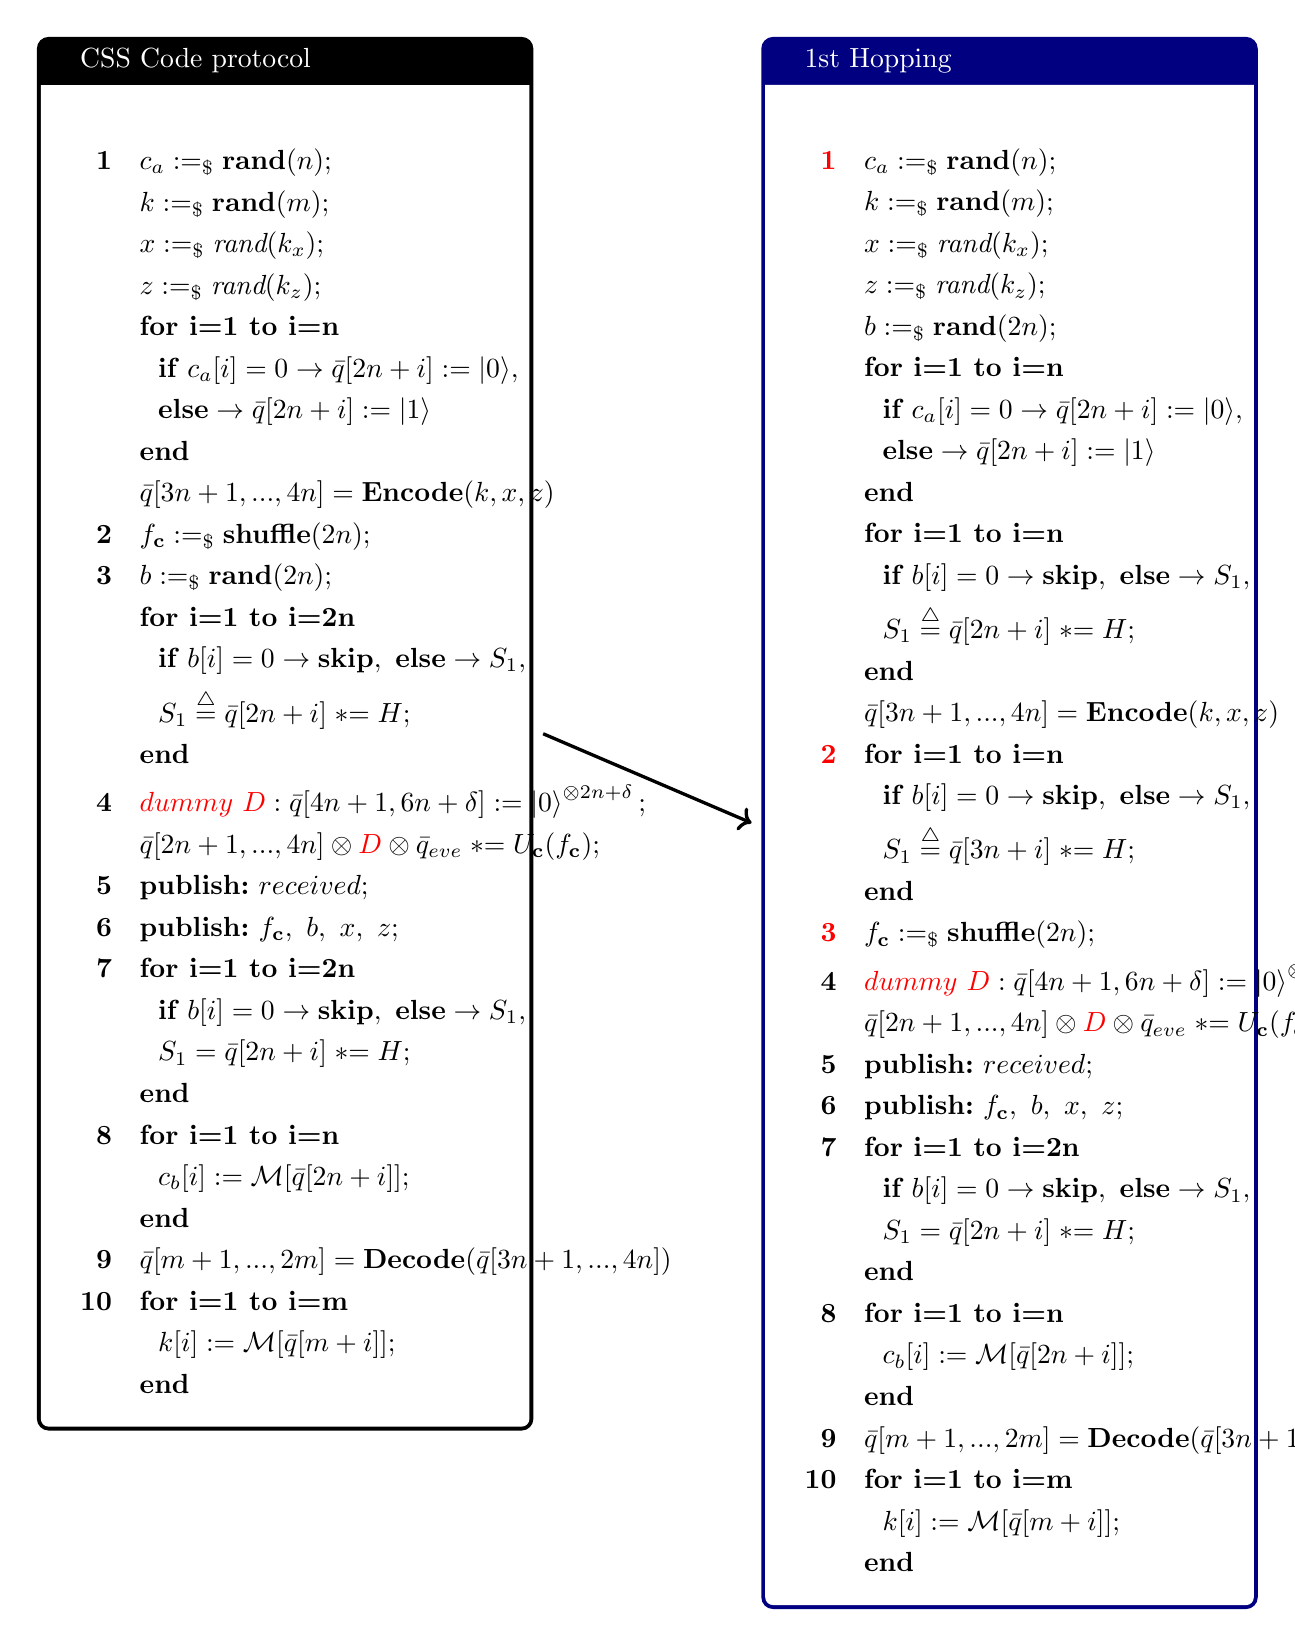
\begin{tikzpicture}[remember picture]

% Left box
\node[anchor=north west] (leftbox) at (0,0) {
\begin{minipage}[t]{0.52\textwidth}
\begin{tcolorbox}[colframe=black!50!black, colback=white, title=CSS Code protocol, width=\textwidth]
\begin{align*}
    \textbf{{1}} \quad 
    & c_a :=_\$ \textbf{rand}(n); \\ 
    & k :=_\$ \textbf{rand}(m); \\ 
    & x :=_\$ \textit{rand}(k_x); \\
    & z :=_\$ \textit{rand}(k_z); \\
    \quad 
    &\textbf{for i=1 to i=n}\\
    &~~ \textbf{if }  c_a[i] = 0 \rightarrow \bar{q}[2n+i] := |0\rangle,\\ &~~\textbf{else}   \rightarrow \bar{q}[2n+i] := |1\rangle\\
    &\textbf{end}\ \\
    \quad 
    &\bar{q}[3n+1,...,4n]=\textbf{Encode}(k,x,z)\\
    \textbf{{2}} \quad & f_{\textbf{c}}:=_\$\textbf{shuffle}(2n); \\
    \textbf{{3}} \quad & b :=_\$ \textbf{rand}(2n); \\
    &\textbf{for i=1 to i=2n}\\
    &~~ \textbf{if }  b[i] = 0 \rightarrow \textbf{skip},~\textbf{else}\rightarrow S_{1} ,\\
    &~~ S_{1}\stackrel{\triangle}{=}\bar{q}[2n+i] \asteq H ;\\
    &\textbf{end}\\
    \textbf{{4}} \quad & \textcolor{red}{dummy~D}: \bar{q}[4n+1,6n+\delta]:=\ket{0}^{\otimes 2n+\delta};\\     &\bar{q}[2n+1,...,4n]\otimes \textcolor{red}{D} \otimes \bar{q}_{eve} \asteq U_{\textbf{c}}(f_{\textbf{c}}); \\
    \textbf{{5}} \quad & \textbf{publish:}~ received;\\
    \textbf{{6}} \quad & \textbf{publish:}~ f_{\textbf{c}},~b,~x,~z;\\
    \textbf{{7}} 
    \quad & \textbf{for i=1 to i=2n}\\
    &~~ \textbf{if }  b[i] = 0 \rightarrow \textbf{skip},~\textbf{else}\rightarrow S_{1} ,\\
    &~~ S_{1}=\bar{q}[2n+i] \asteq H ;\\
    &\textbf{end}\\
    \textbf{{8}} 
    \quad & \textbf{for~i=1~to~i=n}\\
    &~~ c_b[i]:= \mathcal{M} [\bar{q}[2n+i]];\\
    &\textbf{end}\\
    \textbf{{9}} 
    \quad & \bar{q}[m+1,...,2m]=\textbf{Decode}(\bar{q}[3n+1,...,4n])\\
    \textbf{{10}} \quad 
    & \textbf{for~i=1~to~i=m}\\
    &~~ k[i]:= \mathcal{M} [\bar{q}[m+i]];\\
    &\textbf{end}
\end{align*}
\end{tcolorbox}
\end{minipage}
};

% Right box
\node[anchor=north west] (rightbox) at (9.2,0) {
\begin{minipage}[t]{0.52\textwidth}
\begin{tcolorbox}[colframe=blue!50!black, colback=white, title=1st Hopping, width=\textwidth]
\begin{align*}
    \textbf{\textcolor{red}{1}} \quad 
    & c_a :=_\$ \textbf{rand}(n); \\ 
    & k :=_\$ \textbf{rand}(m); \\ 
    & x :=_\$ \textit{rand}(k_x); \\
    & z :=_\$ \textit{rand}(k_z); \\
    & b :=_\$ \textbf{rand}(2n); \\
    \quad 
    &\textbf{for i=1 to i=n}\\
    &~~ \textbf{if }  c_a[i] = 0 \rightarrow \bar{q}[2n+i] := |0\rangle,\\ &~~\textbf{else}   \rightarrow \bar{q}[2n+i] := |1\rangle\\
    &\textbf{end}\ \\
    \quad 
    &\textbf{for i=1 to i=n}\\
    &~~ \textbf{if }  b[i] = 0 \rightarrow \textbf{skip},~\textbf{else}\rightarrow S_{1} ,\\
    &~~ S_{1}\stackrel{\triangle}{=}\bar{q}[2n+i] \asteq H ;\\
    &\textbf{end}\\
    &\bar{q}[3n+1,...,4n]=\textbf{Encode}(k,x,z)\\
    \textbf{\textcolor{red}{2}} \quad 
    &\textbf{for i=1 to i=n}\\
    &~~ \textbf{if }  b[i] = 0 \rightarrow \textbf{skip},~\textbf{else}\rightarrow S_{1} ,\\
    &~~ S_{1}\stackrel{\triangle}{=}\bar{q}[3n+i] \asteq H ;\\
    &\textbf{end}\\
    \textbf{\textcolor{red}{3}} \quad & f_{\textbf{c}}:=_\$\textbf{shuffle}(2n); \\
    \textbf{{4}} \quad & \textcolor{red}{dummy~D}: \bar{q}[4n+1,6n+\delta]:=\ket{0}^{\otimes 2n+\delta};\\     &\bar{q}[2n+1,...,4n]\otimes \textcolor{red}{D} \otimes \bar{q}_{eve} \asteq U_{\textbf{c}}(f_{\textbf{c}}); \\
    \textbf{{5}} \quad & \textbf{publish:}~ received;\\
    \textbf{{6}} \quad & \textbf{publish:}~ f_{\textbf{c}},~b,~x,~z;\\
    \textbf{{7}} 
    \quad & \textbf{for i=1 to i=2n}\\
    &~~ \textbf{if }  b[i] = 0 \rightarrow \textbf{skip},~\textbf{else}\rightarrow S_{1} ,\\
    &~~ S_{1}=\bar{q}[2n+i] \asteq H ;\\
    &\textbf{end}\\
    \textbf{{8}} 
    \quad & \textbf{for~i=1~to~i=n}\\
    &~~ c_b[i]:= \mathcal{M} [\bar{q}[2n+i]];\\
    &\textbf{end}\\
    \textbf{{9}} 
    \quad & \bar{q}[m+1,...,2m]=\textbf{Decode}(\bar{q}[3n+1,...,4n])\\
    \textbf{{10}} \quad 
    & \textbf{for~i=1~to~i=m}\\
    &~~ k[i]:= \mathcal{M} [\bar{q}[m+i]];\\
    &\textbf{end}
\end{align*}
\end{tcolorbox}
\end{minipage}
};

% Draw arrow between boxes
\draw[->, very thick] (leftbox.east) -- node[above]{} (rightbox.west);

\end{tikzpicture}
\newpage
    
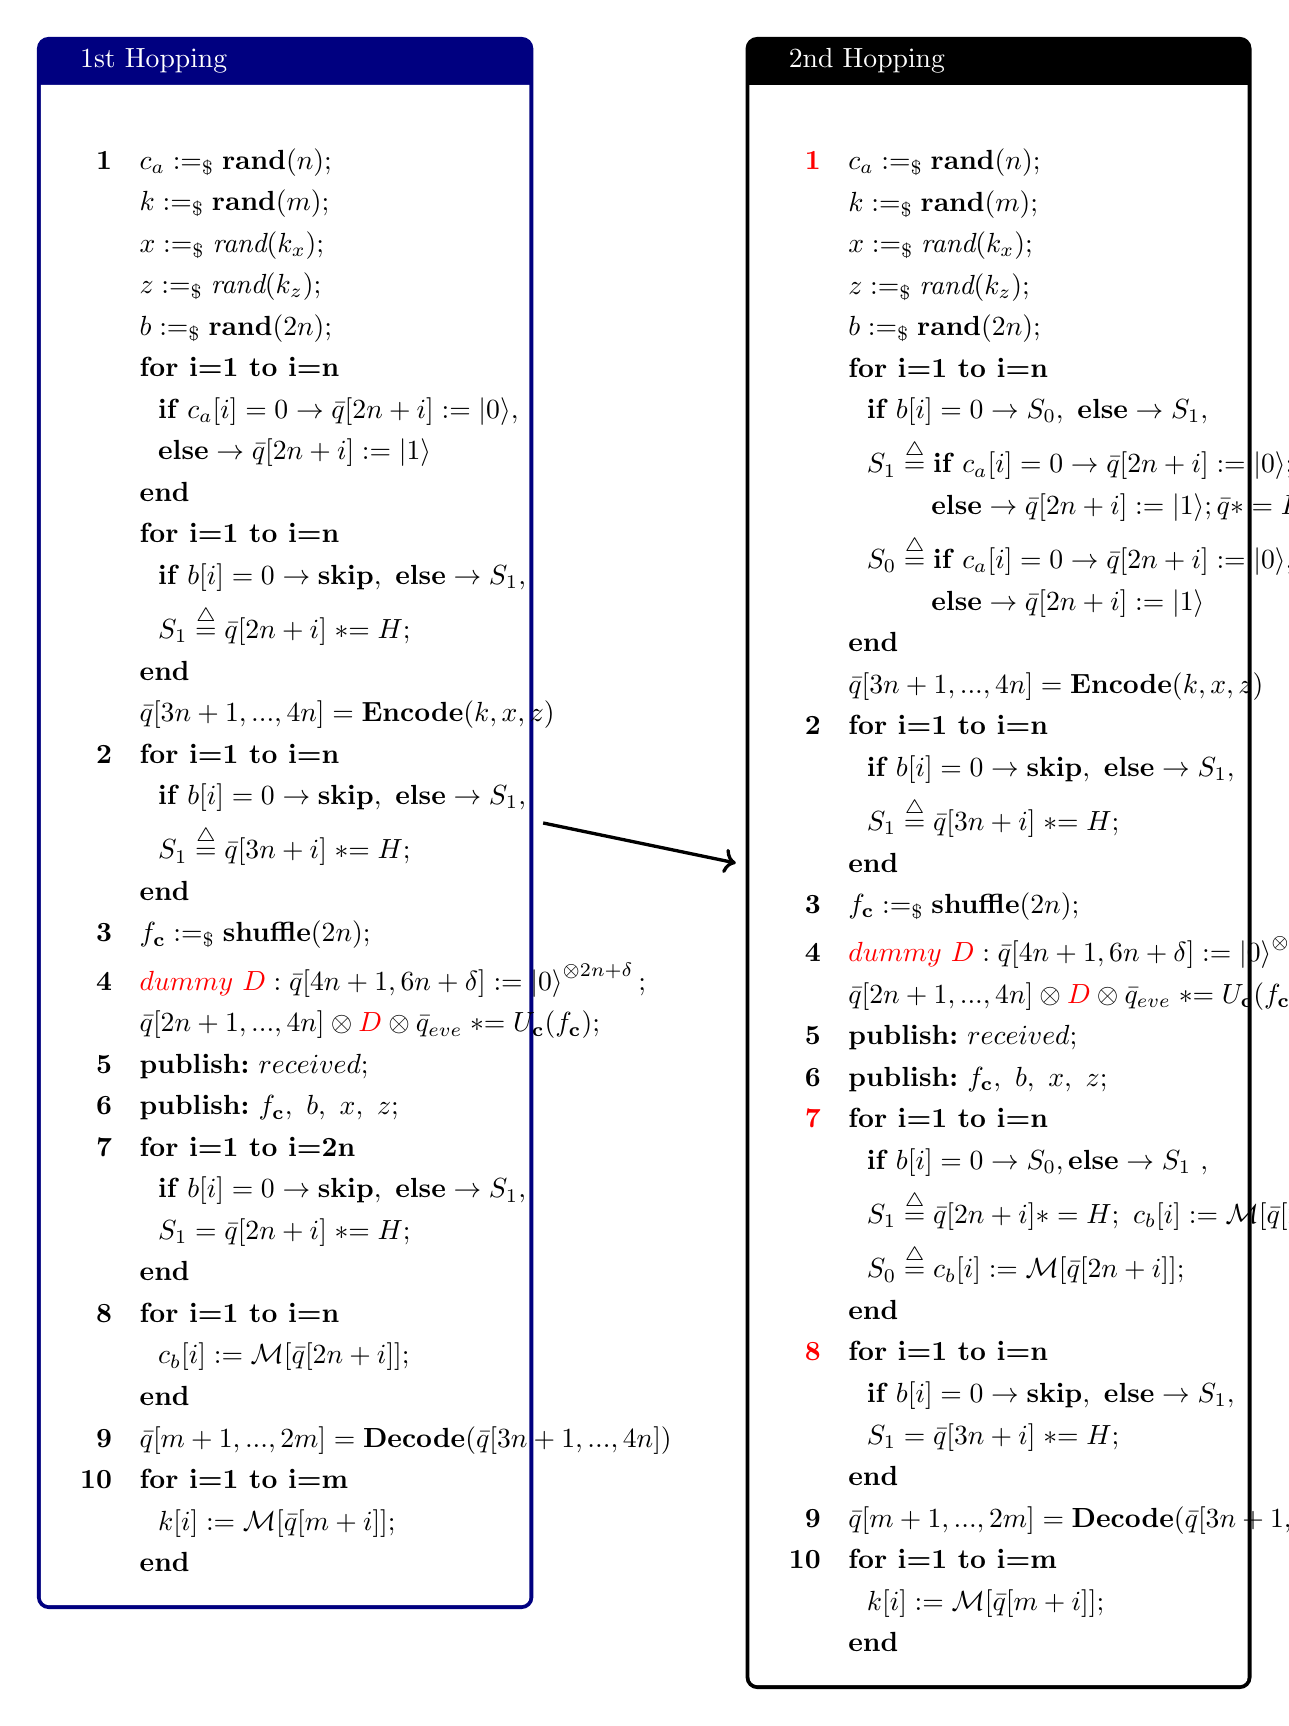
\begin{tikzpicture}[remember picture]

% Left box
\node[anchor=north west] (leftbox) at (0,0) {
\begin{minipage}[t]{0.52\textwidth}
\begin{tcolorbox}[colframe=blue!50!black, colback=white, title=1st Hopping, width=\textwidth]
\begin{align*}
    \textbf{{1}} \quad 
    & c_a :=_\$ \textbf{rand}(n); \\ 
    & k :=_\$ \textbf{rand}(m); \\ 
    & x :=_\$ \textit{rand}(k_x); \\
    & z :=_\$ \textit{rand}(k_z); \\
    & b :=_\$ \textbf{rand}(2n); \\
    \quad 
    &\textbf{for i=1 to i=n}\\
    &~~ \textbf{if }  c_a[i] = 0 \rightarrow \bar{q}[2n+i] := |0\rangle,\\ &~~\textbf{else}   \rightarrow \bar{q}[2n+i] := |1\rangle\\
    &\textbf{end}\ \\
    &\textbf{for i=1 to i=n}\\
    &~~ \textbf{if }  b[i] = 0 \rightarrow \textbf{skip},~\textbf{else}\rightarrow S_{1} ,\\
    &~~ S_{1}\stackrel{\triangle}{=}\bar{q}[2n+i] \asteq H ;\\
    &\textbf{end}\\
    \quad 
    &\bar{q}[3n+1,...,4n]=\textbf{Encode}(k,x,z)\\
    \textbf{{2}} \quad 
    &\textbf{for i=1 to i=n}\\
    &~~ \textbf{if }  b[i] = 0 \rightarrow \textbf{skip},~\textbf{else}\rightarrow S_{1},\\
    &~~ S_{1}\stackrel{\triangle}{=}\bar{q}[3n+i] \asteq H ;\\
    &\textbf{end}\\
    \textbf{{3}} \quad & f_{\textbf{c}}:=_\$\textbf{shuffle}(2n); \\
    \textbf{{4}} \quad & \textcolor{red}{dummy~D}: \bar{q}[4n+1,6n+\delta]:=\ket{0}^{\otimes 2n+\delta};\\     &\bar{q}[2n+1,...,4n]\otimes \textcolor{red}{D} \otimes \bar{q}_{eve} \asteq U_{\textbf{c}}(f_{\textbf{c}}); \\
    \textbf{{5}} \quad & \textbf{publish:}~ received;\\
    \textbf{{6}} \quad & \textbf{publish:}~ f_{\textbf{c}},~b,~x,~z;\\
    \textbf{{7}} 
    \quad & \textbf{for i=1 to i=2n}\\
    &~~ \textbf{if }  b[i] = 0 \rightarrow \textbf{skip},~\textbf{else}\rightarrow S_{1} ,\\
    &~~ S_{1}=\bar{q}[2n+i] \asteq H ;\\
    &\textbf{end}\\
    \textbf{{8}} 
    \quad & \textbf{for~i=1~to~i=n}\\
    &~~ c_b[i]:= \mathcal{M} [\bar{q}[2n+i]];\\
    &\textbf{end}\\
    \textbf{{9}} 
    \quad & \bar{q}[m+1,...,2m]=\textbf{Decode}(\bar{q}[3n+1,...,4n])\\
    \textbf{{10}} \quad 
    & \textbf{for~i=1~to~i=m}\\
    &~~ k[i]:= \mathcal{M} [\bar{q}[m+i]];\\
    &\textbf{end}
\end{align*}
\end{tcolorbox}
\end{minipage}
};

% Right box
\node[anchor=north west] (rightbox) at (9,0) {
\begin{minipage}[t]{0.53\textwidth}
\begin{tcolorbox}[colframe=black!50!black, colback=white, title=2nd Hopping, width=\textwidth]
\begin{align*}
    \textbf{\textcolor{red}{1}} \quad 
    & c_a :=_\$ \textbf{rand}(n); \\ 
    & k :=_\$ \textbf{rand}(m); \\ 
    & x :=_\$ \textit{rand}(k_x); \\
    & z :=_\$ \textit{rand}(k_z); \\
    & b :=_\$ \textbf{rand}(2n); \\
    \quad 
    &\textbf{for i=1 to i=n}\\
    &~~ \textbf{if }  b[i] = 0 \rightarrow S_{0},~\textbf{else}\rightarrow S_{1} ,\\
    &~~ S_{1}\stackrel{\triangle}{=}\textbf{if }  c_a[i] = 0 \rightarrow \bar{q}[2n+i] := |0\rangle;\bar{q}*=H,\\ &~~~~~~~~~\textbf{else}   \rightarrow \bar{q}[2n+i] := |1\rangle;\bar{q}*=H\\
    &~~ S_{0}\stackrel{\triangle}{=}\textbf{if }  c_a[i] = 0 \rightarrow \bar{q}[2n+i] := |0\rangle,\\ &~~~~~~~~~\textbf{else}   \rightarrow \bar{q}[2n+i] := |1\rangle\\
    &\textbf{end}\\\quad 
    &\bar{q}[3n+1,...,4n]=\textbf{Encode}(k,x,z)\\
    \textbf{{2}} \quad 
    &\textbf{for i=1 to i=n}\\
    &~~ \textbf{if }  b[i] = 0 \rightarrow \textbf{skip},~\textbf{else}\rightarrow S_{1} ,\\
    &~~ S_{1}\stackrel{\triangle}{=}\bar{q}[3n+i] \asteq H ;\\
    &\textbf{end}\\
    \textbf{{3}} \quad & f_{\textbf{c}}:=_\$\textbf{shuffle}(2n); \\
    \textbf{{4}} \quad & \textcolor{red}{dummy~D}: \bar{q}[4n+1,6n+\delta]:=\ket{0}^{\otimes 2n+\delta};\\     &\bar{q}[2n+1,...,4n]\otimes \textcolor{red}{D} \otimes \bar{q}_{eve} \asteq U_{\textbf{c}}(f_{\textbf{c}}); \\
    \textbf{{5}} \quad & \textbf{publish:}~ received;\\
    \textbf{{6}} \quad & \textbf{publish:}~ f_{\textbf{c}},~b,~x,~z;\\
    \textbf{\textcolor{red}{7}} 
    \quad 
    &\textbf{for i=1 to i=n}\\
    &~~ \textbf{if }  b[i] = 0 \rightarrow S_{0} ,\textbf{else}\rightarrow S_{1}~,\\
    &~~ S_{1}\stackrel{\triangle}{=}\bar{q}[2n+i]*=H;~c_b[i]:= \mathcal{M}[\bar{q}[2n+i]];\\
    &~~ S_{0}\stackrel{\triangle}{=}c_b[i]:= \mathcal{M}[\bar{q}[2n+i]];\\
    &\textbf{end}\\
    \textbf{\textcolor{red}{8}}\quad 
    &\textbf{for i=1 to i=n}\\
    &~~ \textbf{if }  b[i] = 0 \rightarrow \textbf{skip},~\textbf{else}\rightarrow S_{1} ,\\
    &~~ S_{1}=\bar{q}[3n+i] \asteq H ;\\
    &\textbf{end}\\
    \textbf{{9}} 
    \quad & \bar{q}[m+1,...,2m]=\textbf{Decode}(\bar{q}[3n+1,...,4n])\\
    \textbf{{10}} \quad 
    & \textbf{for~i=1~to~i=m}\\
    &~~ k[i]:= \mathcal{M} [\bar{q}[m+i]];\\
    &\textbf{end}
\end{align*}
\end{tcolorbox}
\end{minipage}
};

% Draw arrow between boxes
\draw[->, very thick] (leftbox.east) -- node[above]{} (rightbox.west);

\end{tikzpicture}
\newpage

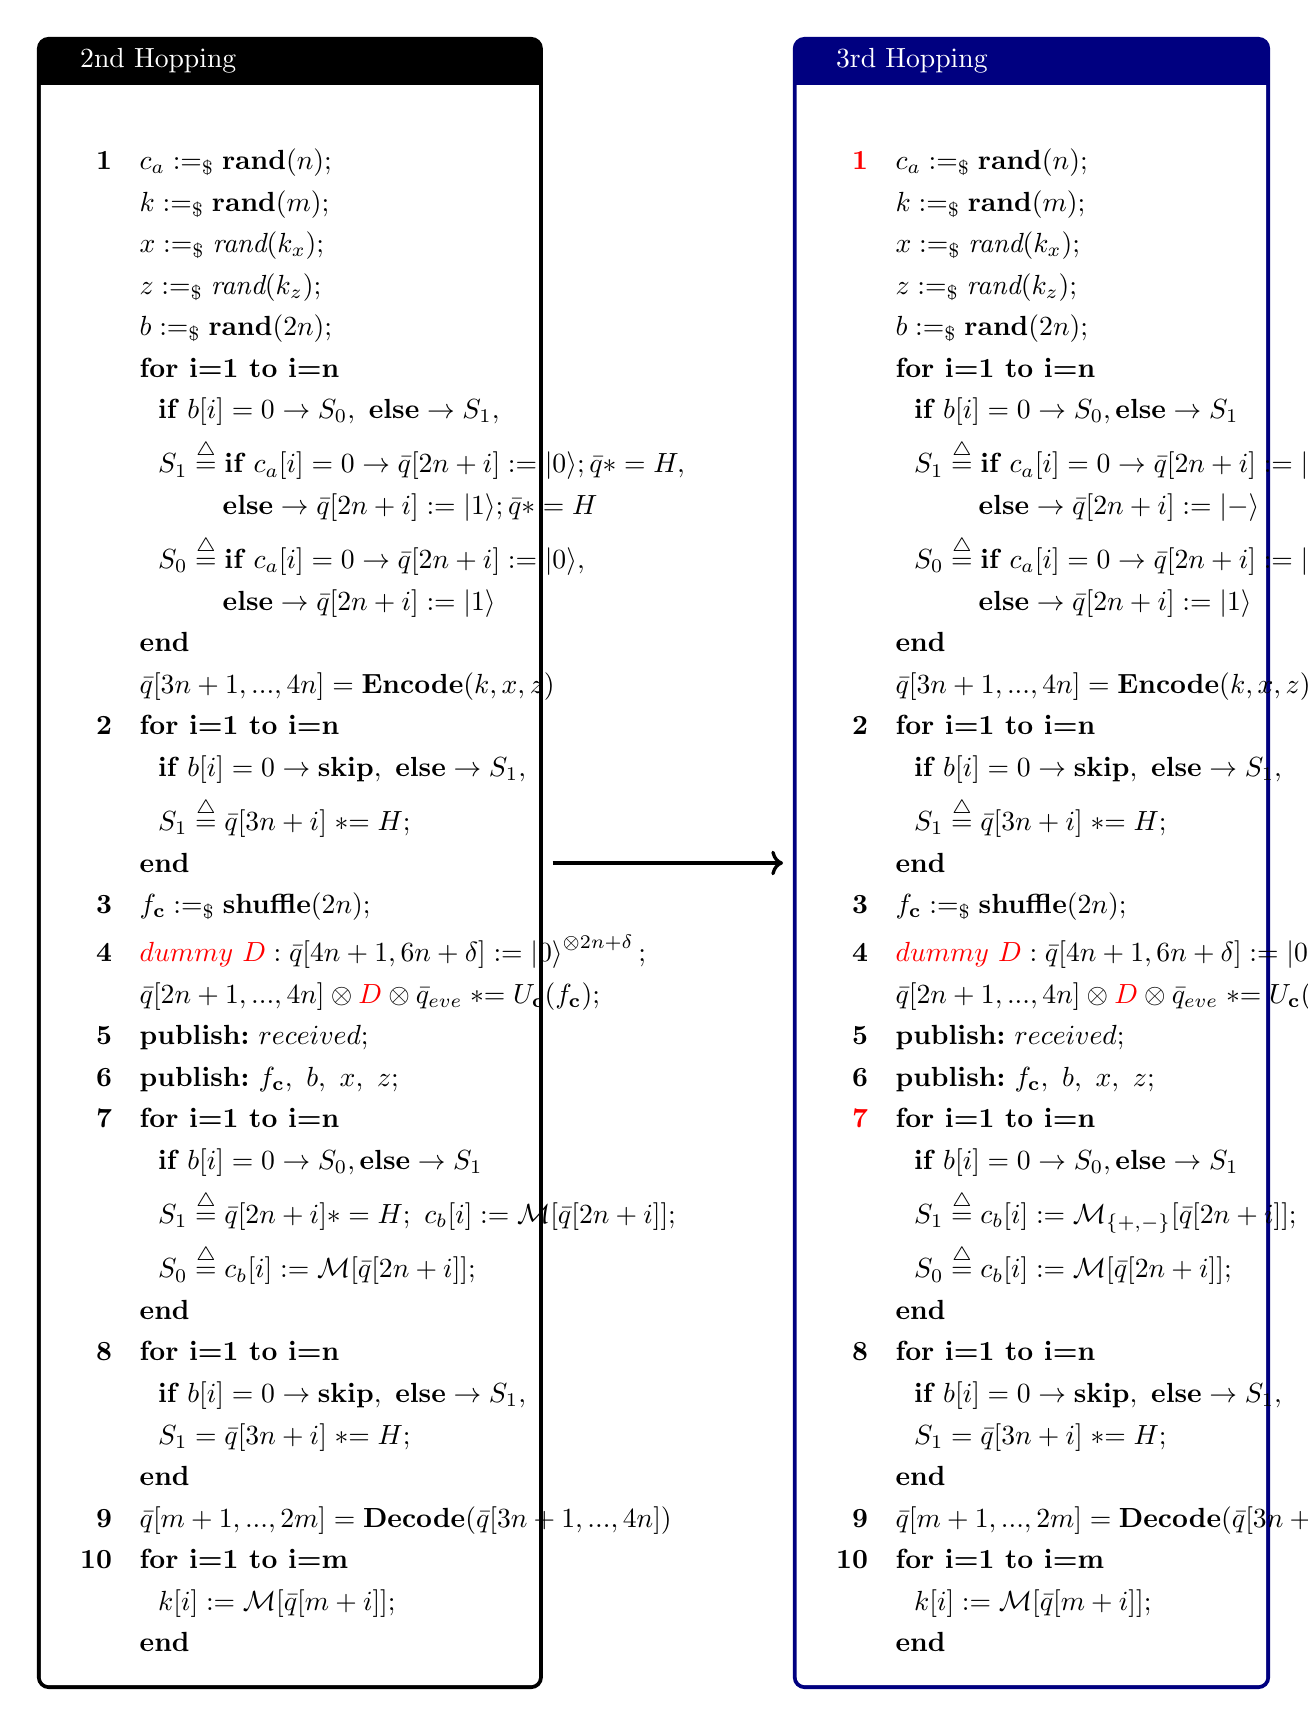
\begin{tikzpicture}[remember picture]

% Left box
\node[anchor=north west] (leftbox) at (0,0) {
\begin{minipage}[t]{0.53\textwidth}
\begin{tcolorbox}[colframe=black!50!black, colback=white, title=2nd Hopping, width=\textwidth]
\begin{align*}
    \textbf{{1}} \quad 
    & c_a :=_\$ \textbf{rand}(n); \\ 
    & k :=_\$ \textbf{rand}(m); \\ 
    & x :=_\$ \textit{rand}(k_x); \\
    & z :=_\$ \textit{rand}(k_z); \\
    & b :=_\$ \textbf{rand}(2n); \\
    \quad 
    &\textbf{for i=1 to i=n}\\
    &~~ \textbf{if }  b[i] = 0 \rightarrow S_{0},~\textbf{else}\rightarrow S_{1} ,\\
    &~~ S_{1}\stackrel{\triangle}{=}\textbf{if }  c_a[i] = 0 \rightarrow \bar{q}[2n+i] := |0\rangle;\bar{q}*=H,\\ &~~~~~~~~~\textbf{else}   \rightarrow \bar{q}[2n+i] := |1\rangle;\bar{q}*=H\\
    &~~ S_{0}\stackrel{\triangle}{=}\textbf{if }  c_a[i] = 0 \rightarrow \bar{q}[2n+i] := |0\rangle,\\ &~~~~~~~~~\textbf{else}   \rightarrow \bar{q}[2n+i] := |1\rangle\\
    &\textbf{end}\\\quad 
    &\bar{q}[3n+1,...,4n]=\textbf{Encode}(k,x,z)\\
    \textbf{{2}} \quad 
    &\textbf{for i=1 to i=n}\\
    &~~ \textbf{if }  b[i] = 0 \rightarrow \textbf{skip},~\textbf{else}\rightarrow S_{1} ,\\
    &~~ S_{1}\stackrel{\triangle}{=}\bar{q}[3n+i] \asteq H ;\\
    &\textbf{end}\\
    \textbf{{3}} \quad & f_{\textbf{c}}:=_\$\textbf{shuffle}(2n); \\
    \textbf{{4}} \quad & \textcolor{red}{dummy~D}: \bar{q}[4n+1,6n+\delta]:=\ket{0}^{\otimes 2n+\delta};\\     &\bar{q}[2n+1,...,4n]\otimes \textcolor{red}{D} \otimes \bar{q}_{eve} \asteq U_{\textbf{c}}(f_{\textbf{c}}); \\
    \textbf{{5}} \quad & \textbf{publish:}~ received;\\
    \textbf{{6}} \quad & \textbf{publish:}~ f_{\textbf{c}},~b,~x,~z;\\
    \textbf{{7}} 
    \quad 
    &\textbf{for i=1 to i=n}\\
    &~~ \textbf{if }  b[i] = 0 \rightarrow S_{0} ,\textbf{else}\rightarrow S_{1}\\
    &~~ S_{1}\stackrel{\triangle}{=}\bar{q}[2n+i]*=H;~c_b[i]:= \mathcal{M}[\bar{q}[2n+i]];\\
    &~~ S_{0}\stackrel{\triangle}{=}c_b[i]:= \mathcal{M}[\bar{q}[2n+i]];\\
    &\textbf{end}\\
    \textbf{{8}}\quad 
    &\textbf{for i=1 to i=n}\\
    &~~ \textbf{if }  b[i] = 0 \rightarrow \textbf{skip},~\textbf{else}\rightarrow S_{1} ,\\
    &~~ S_{1}=\bar{q}[3n+i] \asteq H ;\\
    &\textbf{end}\\
    \textbf{{9}} 
    \quad & \bar{q}[m+1,...,2m]=\textbf{Decode}(\bar{q}[3n+1,...,4n])\\
    \textbf{{10}} \quad 
    & \textbf{for~i=1~to~i=m}\\
    &~~ k[i]:= \mathcal{M} [\bar{q}[m+i]];\\
    &\textbf{end}
\end{align*}
\end{tcolorbox}
\end{minipage}
};

% Right box
\node[anchor=north west] (rightbox) at (9.6,0) {
\begin{minipage}[t]{0.5\textwidth}
\begin{tcolorbox}[colframe=blue!50!black, colback=white, title=3rd Hopping, width=\textwidth]
\begin{align*}
    \textbf{\textcolor{red}{1}} \quad 
    & c_a :=_\$ \textbf{rand}(n); \\ 
    & k :=_\$ \textbf{rand}(m); \\ 
    & x :=_\$ \textit{rand}(k_x); \\
    & z :=_\$ \textit{rand}(k_z); \\
    & b :=_\$ \textbf{rand}(2n); \\
    \quad 
    &\textbf{for i=1 to i=n}\\
    &~~ \textbf{if }  b[i] = 0 \rightarrow S_{0} ,\textbf{else}\rightarrow S_{1}\\
    &~~ S_{1}\stackrel{\triangle}{=}\textbf{if }  c_a[i] = 0 \rightarrow \bar{q}[2n+i] := |+\rangle,\\ &~~~~~~~~~\textbf{else}   \rightarrow \bar{q}[2n+i] := |-\rangle\\
    &~~ S_{0}\stackrel{\triangle}{=}\textbf{if }  c_a[i] = 0 \rightarrow \bar{q}[2n+i] := |0\rangle,\\ &~~~~~~~~~\textbf{else}   \rightarrow \bar{q}[2n+i] := |1\rangle\\
    &\textbf{end}\\\quad 
    &\bar{q}[3n+1,...,4n]=\textbf{Encode}(k,x,z)\\
    \textbf{{2}} \quad 
    &\textbf{for i=1 to i=n}\\
    &~~ \textbf{if }  b[i] = 0 \rightarrow \textbf{skip},~\textbf{else}\rightarrow S_{1} ,\\
    &~~ S_{1}\stackrel{\triangle}{=}\bar{q}[3n+i] \asteq H ;\\
    &\textbf{end}\\
    \textbf{{3}} \quad & f_{\textbf{c}}:=_\$\textbf{shuffle}(2n); \\
    \textbf{{4}} \quad & \textcolor{red}{dummy~D}: \bar{q}[4n+1,6n+\delta]:=\ket{0}^{\otimes 2n+\delta};\\     &\bar{q}[2n+1,...,4n]\otimes \textcolor{red}{D} \otimes \bar{q}_{eve} \asteq U_{\textbf{c}}(f_{\textbf{c}}); \\
    \textbf{{5}} \quad & \textbf{publish:}~ received;\\
    \textbf{{6}} \quad & \textbf{publish:}~ f_{\textbf{c}},~b,~x,~z;\\
    \textbf{\textcolor{red}{7}} 
    \quad 
    &\textbf{for i=1 to i=n}\\
    &~~ \textbf{if }  b[i] = 0 \rightarrow S_{0} ,\textbf{else}\rightarrow S_{1}\\
    &~~ S_{1}\stackrel{\triangle}{=}c_b[i]:= \mathcal{M}_{\{+,-\}} [\bar{q}[2n+i]];\\
    &~~ S_{0}\stackrel{\triangle}{=}c_b[i]:= \mathcal{M} [\bar{q}[2n+i]];\\
    &\textbf{end}\\
    \textbf{{8}}\quad 
    &\textbf{for i=1 to i=n}\\
    &~~ \textbf{if }  b[i] = 0 \rightarrow \textbf{skip},~\textbf{else}\rightarrow S_{1} ,\\
    &~~ S_{1}=\bar{q}[3n+i] \asteq H ;\\
    &\textbf{end}\\
    \textbf{{9}} 
    \quad & \bar{q}[m+1,...,2m]=\textbf{Decode}(\bar{q}[3n+1,...,4n])\\
    \textbf{{10}} \quad 
    & \textbf{for~i=1~to~i=m}\\
    &~~ k[i]:= \mathcal{M} [\bar{q}[m+i]];\\
    &\textbf{end}
\end{align*}
\end{tcolorbox}
\end{minipage}
};

% Draw arrow between boxes
\draw[->, very thick] (leftbox.east) -- node[above]{} (rightbox.west);

\end{tikzpicture}
\newpage


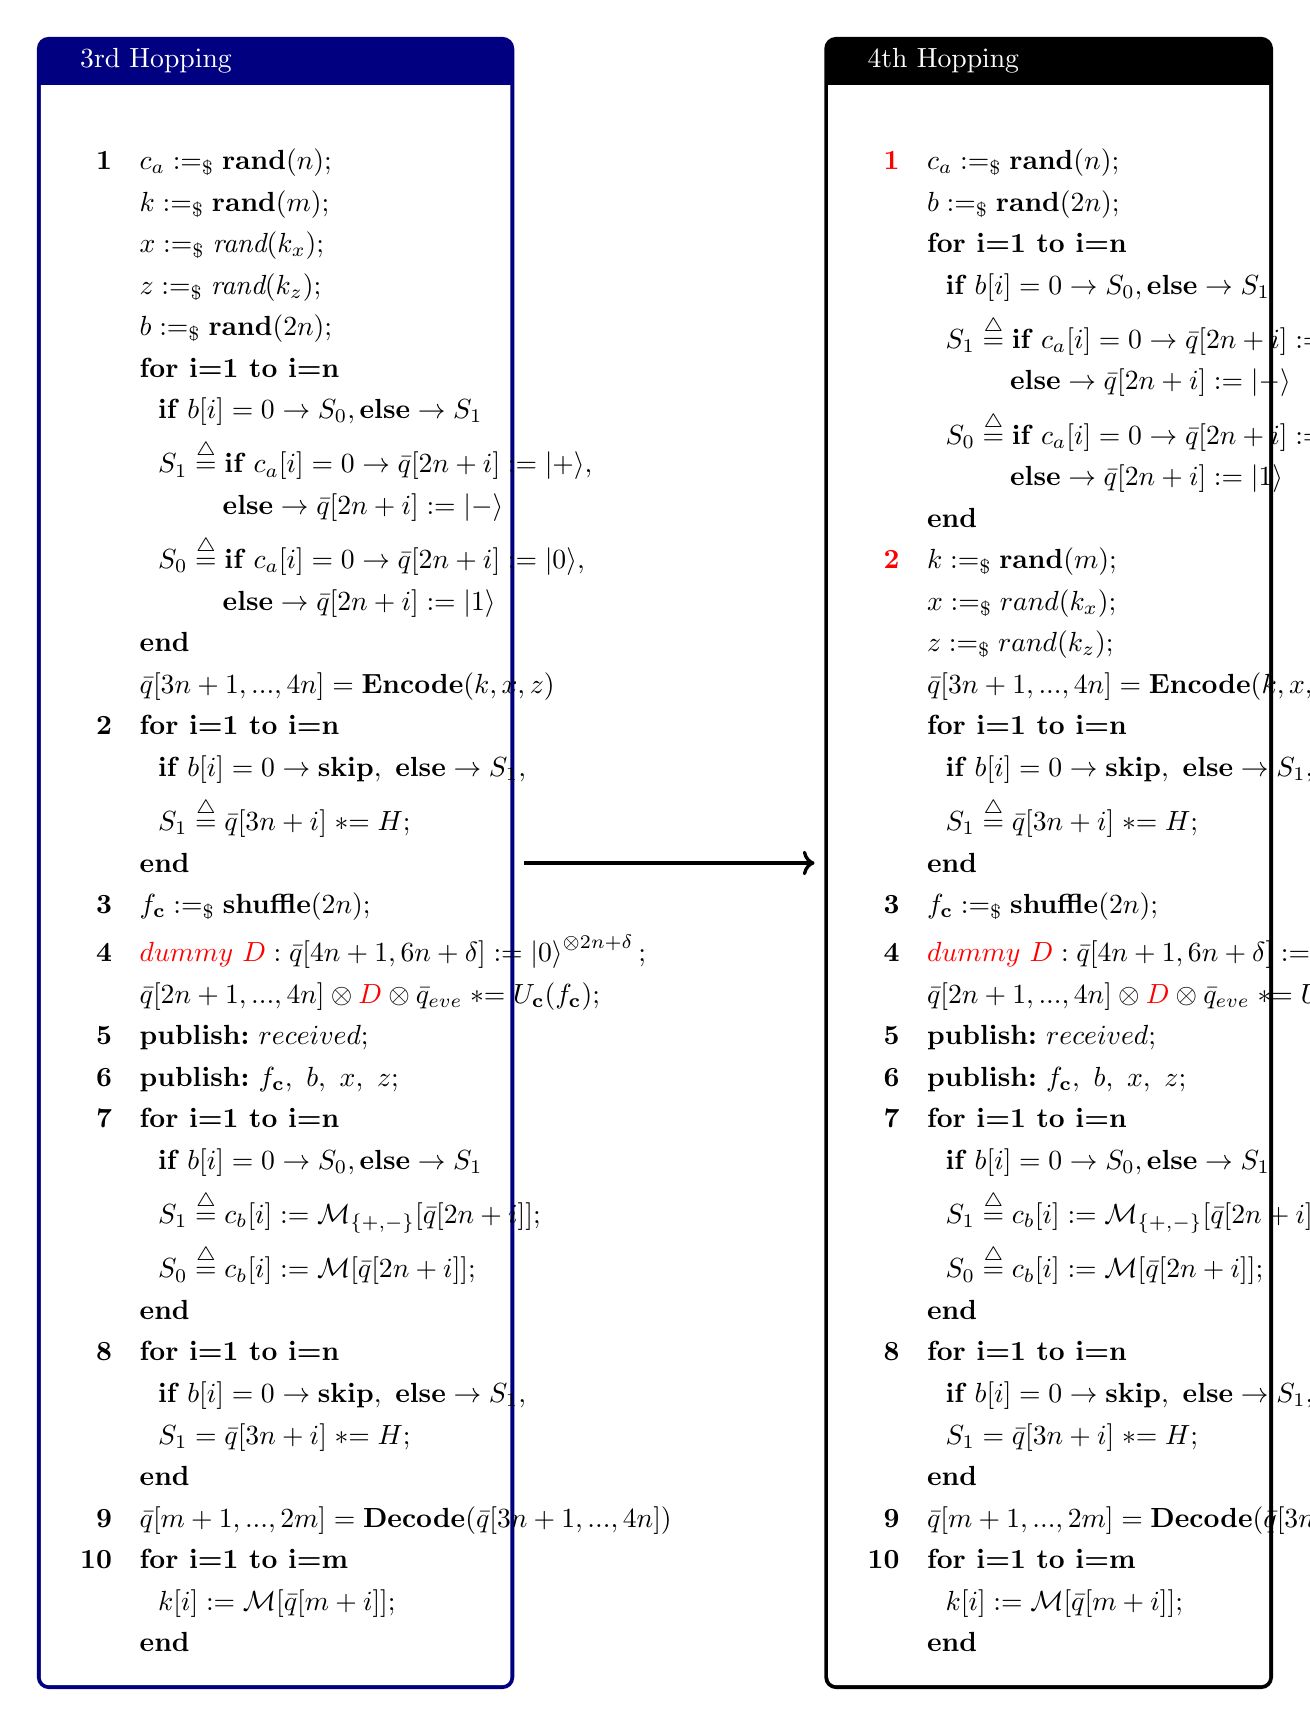
\begin{tikzpicture}[remember picture]

% Left box
\node[anchor=north west] (leftbox) at (0,0) {
\begin{minipage}[t]{0.5\textwidth}
\begin{tcolorbox}[colframe=blue!50!black, colback=white, title=3rd Hopping, width=\textwidth]
\begin{align*}
    \textbf{{1}} \quad 
    & c_a :=_\$ \textbf{rand}(n); \\ 
    & k :=_\$ \textbf{rand}(m); \\ 
    & x :=_\$ \textit{rand}(k_x); \\
    & z :=_\$ \textit{rand}(k_z); \\
    & b :=_\$ \textbf{rand}(2n); \\
    \quad 
    &\textbf{for i=1 to i=n}\\
    &~~ \textbf{if }  b[i] = 0 \rightarrow S_{0} ,\textbf{else}\rightarrow S_{1}\\
    &~~ S_{1}\stackrel{\triangle}{=}\textbf{if }  c_a[i] = 0 \rightarrow \bar{q}[2n+i] := |+\rangle,\\ &~~~~~~~~~\textbf{else}   \rightarrow \bar{q}[2n+i] := |-\rangle\\
    &~~ S_{0}\stackrel{\triangle}{=}\textbf{if }  c_a[i] = 0 \rightarrow \bar{q}[2n+i] := |0\rangle,\\ &~~~~~~~~~\textbf{else}   \rightarrow \bar{q}[2n+i] := |1\rangle\\
    &\textbf{end}\\\quad 
    &\bar{q}[3n+1,...,4n]=\textbf{Encode}(k,x,z)\\
    \textbf{{2}} \quad 
    &\textbf{for i=1 to i=n}\\
    &~~ \textbf{if }  b[i] = 0 \rightarrow \textbf{skip},~\textbf{else}\rightarrow S_{1} ,\\
    &~~ S_{1}\stackrel{\triangle}{=}\bar{q}[3n+i] \asteq H ;\\
    &\textbf{end}\\
    \textbf{{3}} \quad & f_{\textbf{c}}:=_\$\textbf{shuffle}(2n); \\
    \textbf{{4}} \quad & \textcolor{red}{dummy~D}: \bar{q}[4n+1,6n+\delta]:=\ket{0}^{\otimes 2n+\delta};\\     &\bar{q}[2n+1,...,4n]\otimes \textcolor{red}{D} \otimes \bar{q}_{eve} \asteq U_{\textbf{c}}(f_{\textbf{c}}); \\
    \textbf{{5}} \quad & \textbf{publish:}~ received;\\
    \textbf{{6}} \quad & \textbf{publish:}~ f_{\textbf{c}},~b,~x,~z;\\
    \textbf{{7}} 
    \quad 
    &\textbf{for i=1 to i=n}\\
    &~~ \textbf{if }  b[i] = 0 \rightarrow S_{0} ,\textbf{else}\rightarrow S_{1}\\
    &~~ S_{1}\stackrel{\triangle}{=}c_b[i]:= \mathcal{M}_{\{+,-\}} [\bar{q}[2n+i]];\\
    &~~ S_{0}\stackrel{\triangle}{=}c_b[i]:= \mathcal{M} [\bar{q}[2n+i]];\\
    &\textbf{end}\\
    \textbf{{8}}\quad 
    &\textbf{for i=1 to i=n}\\
    &~~ \textbf{if }  b[i] = 0 \rightarrow \textbf{skip},~\textbf{else}\rightarrow S_{1} ,\\
    &~~ S_{1}=\bar{q}[3n+i] \asteq H ;\\
    &\textbf{end}\\
    \textbf{{9}} 
    \quad & \bar{q}[m+1,...,2m]=\textbf{Decode}(\bar{q}[3n+1,...,4n])\\
    \textbf{{10}} \quad 
    & \textbf{for~i=1~to~i=m}\\
    &~~ k[i]:= \mathcal{M} [\bar{q}[m+i]];\\
    &\textbf{end}
\end{align*}
\end{tcolorbox}
\end{minipage}
};

% Right box
\node[anchor=north west] (rightbox) at (10,0) {
\begin{minipage}[t]{0.47\textwidth}
\begin{tcolorbox}[colframe=black!50!black, colback=white, title=4th Hopping, width=\textwidth]
\begin{align*}
    \textbf{\textcolor{red}{1}} \quad 
    & c_a :=_\$ \textbf{rand}(n); \\ 
    & b :=_\$ \textbf{rand}(2n); \\
    &\textbf{for i=1 to i=n}\\
    &~~ \textbf{if }  b[i] = 0 \rightarrow S_{0} ,\textbf{else}\rightarrow S_{1}\\
    &~~ S_{1}\stackrel{\triangle}{=}\textbf{if }  c_a[i] = 0 \rightarrow \bar{q}[2n+i] := |+\rangle,\\ &~~~~~~~~~\textbf{else}   \rightarrow \bar{q}[2n+i] := |-\rangle\\
    &~~ S_{0}\stackrel{\triangle}{=}\textbf{if }  c_a[i] = 0 \rightarrow \bar{q}[2n+i] := |0\rangle,\\ &~~~~~~~~~\textbf{else}   \rightarrow \bar{q}[2n+i] := |1\rangle\\
    &\textbf{end}\\
    \textbf{\textcolor{red}{2}}\quad 
    & k :=_\$ \textbf{rand}(m); \\
    & x :=_\$ {rand}(k_x); \\
    & z :=_\$ {rand}(k_z); \\
    &\bar{q}[3n+1,...,4n]=\textbf{Encode}(k,x,z)\\
    &\textbf{for i=1 to i=n}\\
    &~~ \textbf{if }  b[i] = 0 \rightarrow \textbf{skip},~\textbf{else}\rightarrow S_{1} ,\\
    &~~ S_{1}\stackrel{\triangle}{=}\bar{q}[3n+i] \asteq H ;\\
    &\textbf{end}\\
    \textbf{{3}} \quad & f_{\textbf{c}}:=_\$\textbf{shuffle}(2n); \\
    \textbf{{4}} \quad & \textcolor{red}{dummy~D}: \bar{q}[4n+1,6n+\delta]:=\ket{0}^{\otimes 2n+\delta};\\     &\bar{q}[2n+1,...,4n]\otimes \textcolor{red}{D} \otimes \bar{q}_{eve} \asteq U_{\textbf{c}}(f_{\textbf{c}}); \\
    \textbf{{5}} \quad & \textbf{publish:}~ received;\\
    \textbf{{6}} \quad & \textbf{publish:}~ f_{\textbf{c}},~b,~x,~z;\\
    \textbf{{7}} 
    \quad 
    &\textbf{for i=1 to i=n}\\
    &~~ \textbf{if }  b[i] = 0 \rightarrow S_{0} ,\textbf{else}\rightarrow S_{1}\\
    &~~ S_{1}\stackrel{\triangle}{=}c_b[i]:= \mathcal{M}_{\{+,-\}} [\bar{q}[2n+i]];\\
    &~~ S_{0}\stackrel{\triangle}{=}c_b[i]:= \mathcal{M} [\bar{q}[2n+i]];\\
    &\textbf{end}\\
    \textbf{{8}}\quad 
    &\textbf{for i=1 to i=n}\\
    &~~ \textbf{if }  b[i] = 0 \rightarrow \textbf{skip},~\textbf{else}\rightarrow S_{1} ,\\
    &~~ S_{1}=\bar{q}[3n+i] \asteq H ;\\
    &\textbf{end}\\
    \textbf{{9}} 
    \quad & \bar{q}[m+1,...,2m]=\textbf{Decode}(\bar{q}[3n+1,...)\\
    \textbf{{10}} \quad 
    & \textbf{for~i=1~to~i=m}\\
    &~~ k[i]:= \mathcal{M} [\bar{q}[m+i]];\\
    &\textbf{end}
\end{align*}
\end{tcolorbox}
\end{minipage}
};

% Draw arrow between boxes
\draw[->, very thick] (leftbox.east) -- node[above]{} (rightbox.west);

\end{tikzpicture}
\newpage

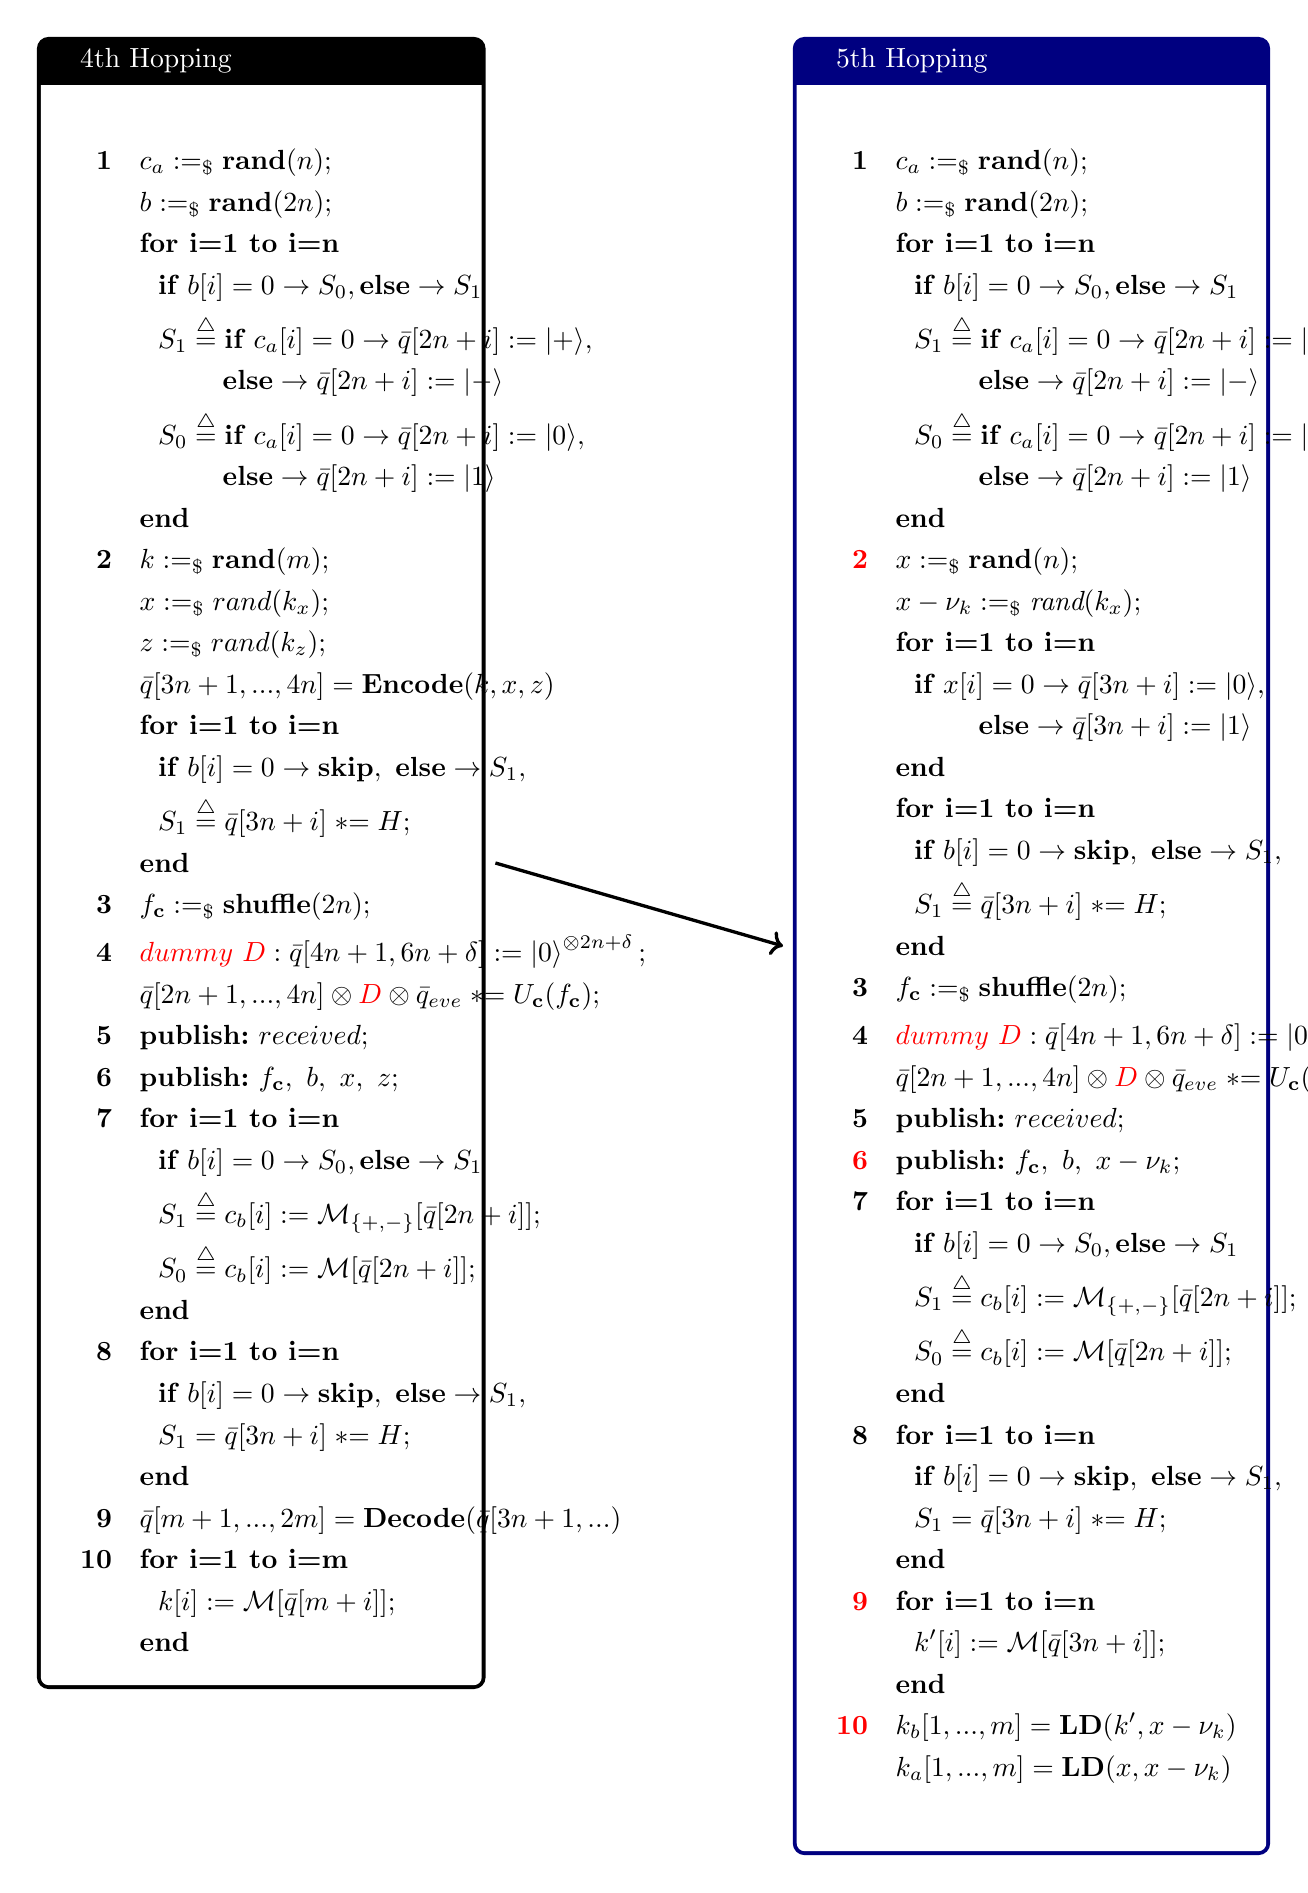
\begin{tikzpicture}[remember picture]

% Left box
\node[anchor=north west] (leftbox) at (0,0) {
\begin{minipage}[t]{0.47\textwidth}
\begin{tcolorbox}[colframe=black!50!black, colback=white, title=4th Hopping, width=\textwidth]
\begin{align*}
    \textbf{{1}} \quad 
    & c_a :=_\$ \textbf{rand}(n); \\ 
    & b :=_\$ \textbf{rand}(2n); \\
    &\textbf{for i=1 to i=n}\\
    &~~ \textbf{if }  b[i] = 0 \rightarrow S_{0} ,\textbf{else}\rightarrow S_{1}\\
    &~~ S_{1}\stackrel{\triangle}{=}\textbf{if }  c_a[i] = 0 \rightarrow \bar{q}[2n+i] := |+\rangle,\\ &~~~~~~~~~\textbf{else}   \rightarrow \bar{q}[2n+i] := |-\rangle\\
    &~~ S_{0}\stackrel{\triangle}{=}\textbf{if }  c_a[i] = 0 \rightarrow \bar{q}[2n+i] := |0\rangle,\\ &~~~~~~~~~\textbf{else}   \rightarrow \bar{q}[2n+i] := |1\rangle\\
    &\textbf{end}\\
    \textbf{{2}}\quad 
    & k :=_\$ \textbf{rand}(m); \\
    & x :=_\$ {rand}(k_x); \\
    & z :=_\$ {rand}(k_z); \\
    &\bar{q}[3n+1,...,4n]=\textbf{Encode}(k,x,z)\\
    &\textbf{for i=1 to i=n}\\
    &~~ \textbf{if }  b[i] = 0 \rightarrow \textbf{skip},~\textbf{else}\rightarrow S_{1} ,\\
    &~~ S_{1}\stackrel{\triangle}{=}\bar{q}[3n+i] \asteq H ;\\
    &\textbf{end}\\
    \textbf{{3}} \quad & f_{\textbf{c}}:=_\$\textbf{shuffle}(2n); \\
    \textbf{{4}} \quad & \textcolor{red}{dummy~D}: \bar{q}[4n+1,6n+\delta]:=\ket{0}^{\otimes 2n+\delta};\\     &\bar{q}[2n+1,...,4n]\otimes \textcolor{red}{D} \otimes \bar{q}_{eve} \asteq U_{\textbf{c}}(f_{\textbf{c}}); \\
    \textbf{{5}} \quad & \textbf{publish:}~ received;\\
    \textbf{{6}} \quad & \textbf{publish:}~ f_{\textbf{c}},~b,~x,~z;\\
    \textbf{{7}} 
    \quad 
    &\textbf{for i=1 to i=n}\\
    &~~ \textbf{if }  b[i] = 0 \rightarrow S_{0} ,\textbf{else}\rightarrow S_{1}\\
    &~~ S_{1}\stackrel{\triangle}{=}c_b[i]:= \mathcal{M}_{\{+,-\}} [\bar{q}[2n+i]];\\
    &~~ S_{0}\stackrel{\triangle}{=}c_b[i]:= \mathcal{M} [\bar{q}[2n+i]];\\
    &\textbf{end}\\
    \textbf{{8}}\quad 
    &\textbf{for i=1 to i=n}\\
    &~~ \textbf{if }  b[i] = 0 \rightarrow \textbf{skip},~\textbf{else}\rightarrow S_{1} ,\\
    &~~ S_{1}=\bar{q}[3n+i] \asteq H ;\\
    &\textbf{end}\\
    \textbf{{9}} 
    \quad & \bar{q}[m+1,...,2m]=\textbf{Decode}(\bar{q}[3n+1,...)\\
    \textbf{{10}} \quad 
    & \textbf{for~i=1~to~i=m}\\
    &~~ k[i]:= \mathcal{M} [\bar{q}[m+i]];\\
    &\textbf{end}
\end{align*}
\end{tcolorbox}
\end{minipage}
};

% Right box
\node[anchor=north west] (rightbox) at (9.6,0) {
\begin{minipage}[t]{0.5\textwidth}
\begin{tcolorbox}[colframe=blue!50!black, colback=white, title=5th Hopping, width=\textwidth]
\begin{align*}
    \textbf{{1}} \quad 
    & c_a :=_\$ \textbf{rand}(n); \\ 
    & b :=_\$ \textbf{rand}(2n); \\
    \quad 
    &\textbf{for i=1 to i=n}\\
    &~~ \textbf{if }  b[i] = 0 \rightarrow S_{0} ,\textbf{else}\rightarrow S_{1}\\
    &~~ S_{1}\stackrel{\triangle}{=}\textbf{if }  c_a[i] = 0 \rightarrow \bar{q}[2n+i] := |+\rangle,\\ &~~~~~~~~~\textbf{else}   \rightarrow \bar{q}[2n+i] := |-\rangle\\
    &~~ S_{0}\stackrel{\triangle}{=}\textbf{if }  c_a[i] = 0 \rightarrow \bar{q}[2n+i] := |0\rangle,\\ &~~~~~~~~~\textbf{else}   \rightarrow \bar{q}[2n+i] := |1\rangle\\
    &\textbf{end}\\
    \textbf{\textcolor{red}{2}}\quad 
    & x :=_\$ \textbf{rand}(n); \\
    & x-\nu_k :=_\$ \textit{rand}(k_x);\\
    &\textbf{for i=1 to i=n}\\
    &~~ \textbf{if }  x[i] = 0 \rightarrow \bar{q}[3n+i] := |0\rangle,\\ &~~~~~~~~~\textbf{else}   \rightarrow \bar{q}[3n+i] := |1\rangle\\
    &\textbf{end}\\
    &\textbf{for i=1 to i=n}\\
    &~~ \textbf{if }  b[i] = 0 \rightarrow \textbf{skip},~\textbf{else}\rightarrow S_{1} ,\\
    &~~ S_{1}\stackrel{\triangle}{=}\bar{q}[3n+i] \asteq H ;\\
    &\textbf{end}\\
    \textbf{{3}} \quad & f_{\textbf{c}}:=_\$\textbf{shuffle}(2n); \\
    \textbf{{4}} \quad & \textcolor{red}{dummy~D}: \bar{q}[4n+1,6n+\delta]:=\ket{0}^{\otimes 2n+\delta};\\     &\bar{q}[2n+1,...,4n]\otimes \textcolor{red}{D} \otimes \bar{q}_{eve} \asteq U_{\textbf{c}}(f_{\textbf{c}}); \\
    \textbf{{5}} \quad & \textbf{publish:}~ received;\\
    \textbf{\textcolor{red}{6}} \quad & \textbf{publish:}~ f_{\textbf{c}},~b,~x-\nu_k;\\
    \textbf{{7}} 
    \quad 
    &\textbf{for i=1 to i=n}\\
    &~~ \textbf{if }  b[i] = 0 \rightarrow S_{0} ,\textbf{else}\rightarrow S_{1}\\
    &~~ S_{1}\stackrel{\triangle}{=}c_b[i]:= \mathcal{M}_{\{+,-\}} [\bar{q}[2n+i]];\\
    &~~ S_{0}\stackrel{\triangle}{=}c_b[i]:= \mathcal{M} [\bar{q}[2n+i]];\\
    &\textbf{end}\\
    \textbf{{8}}\quad 
    &\textbf{for i=1 to i=n}\\
    &~~ \textbf{if }  b[i] = 0 \rightarrow \textbf{skip},~\textbf{else}\rightarrow S_{1} ,\\
    &~~ S_{1}=\bar{q}[3n+i] \asteq H ;\\
    &\textbf{end}\\
    \textbf{\textcolor{red}{9}} \quad 
    &\textbf{for i=1 to i=n}\\
    &~~ k'[i]:= \mathcal{M} [\bar{q}[3n+i]];\\
    &\textbf{end}\\
    \textcolor{red}{\textbf{10}} \quad & k_b[1,...,m]=\textbf{LD}(k',x-\nu_k)\\
    &k_a[1,...,m]=\textbf{LD}(x,x-\nu_k)\\
\end{align*}
\end{tcolorbox}
\end{minipage}
};

% Draw arrow between boxes
\draw[->, very thick] (leftbox.east) -- node[above]{} (rightbox.west);

\end{tikzpicture}
\newpage

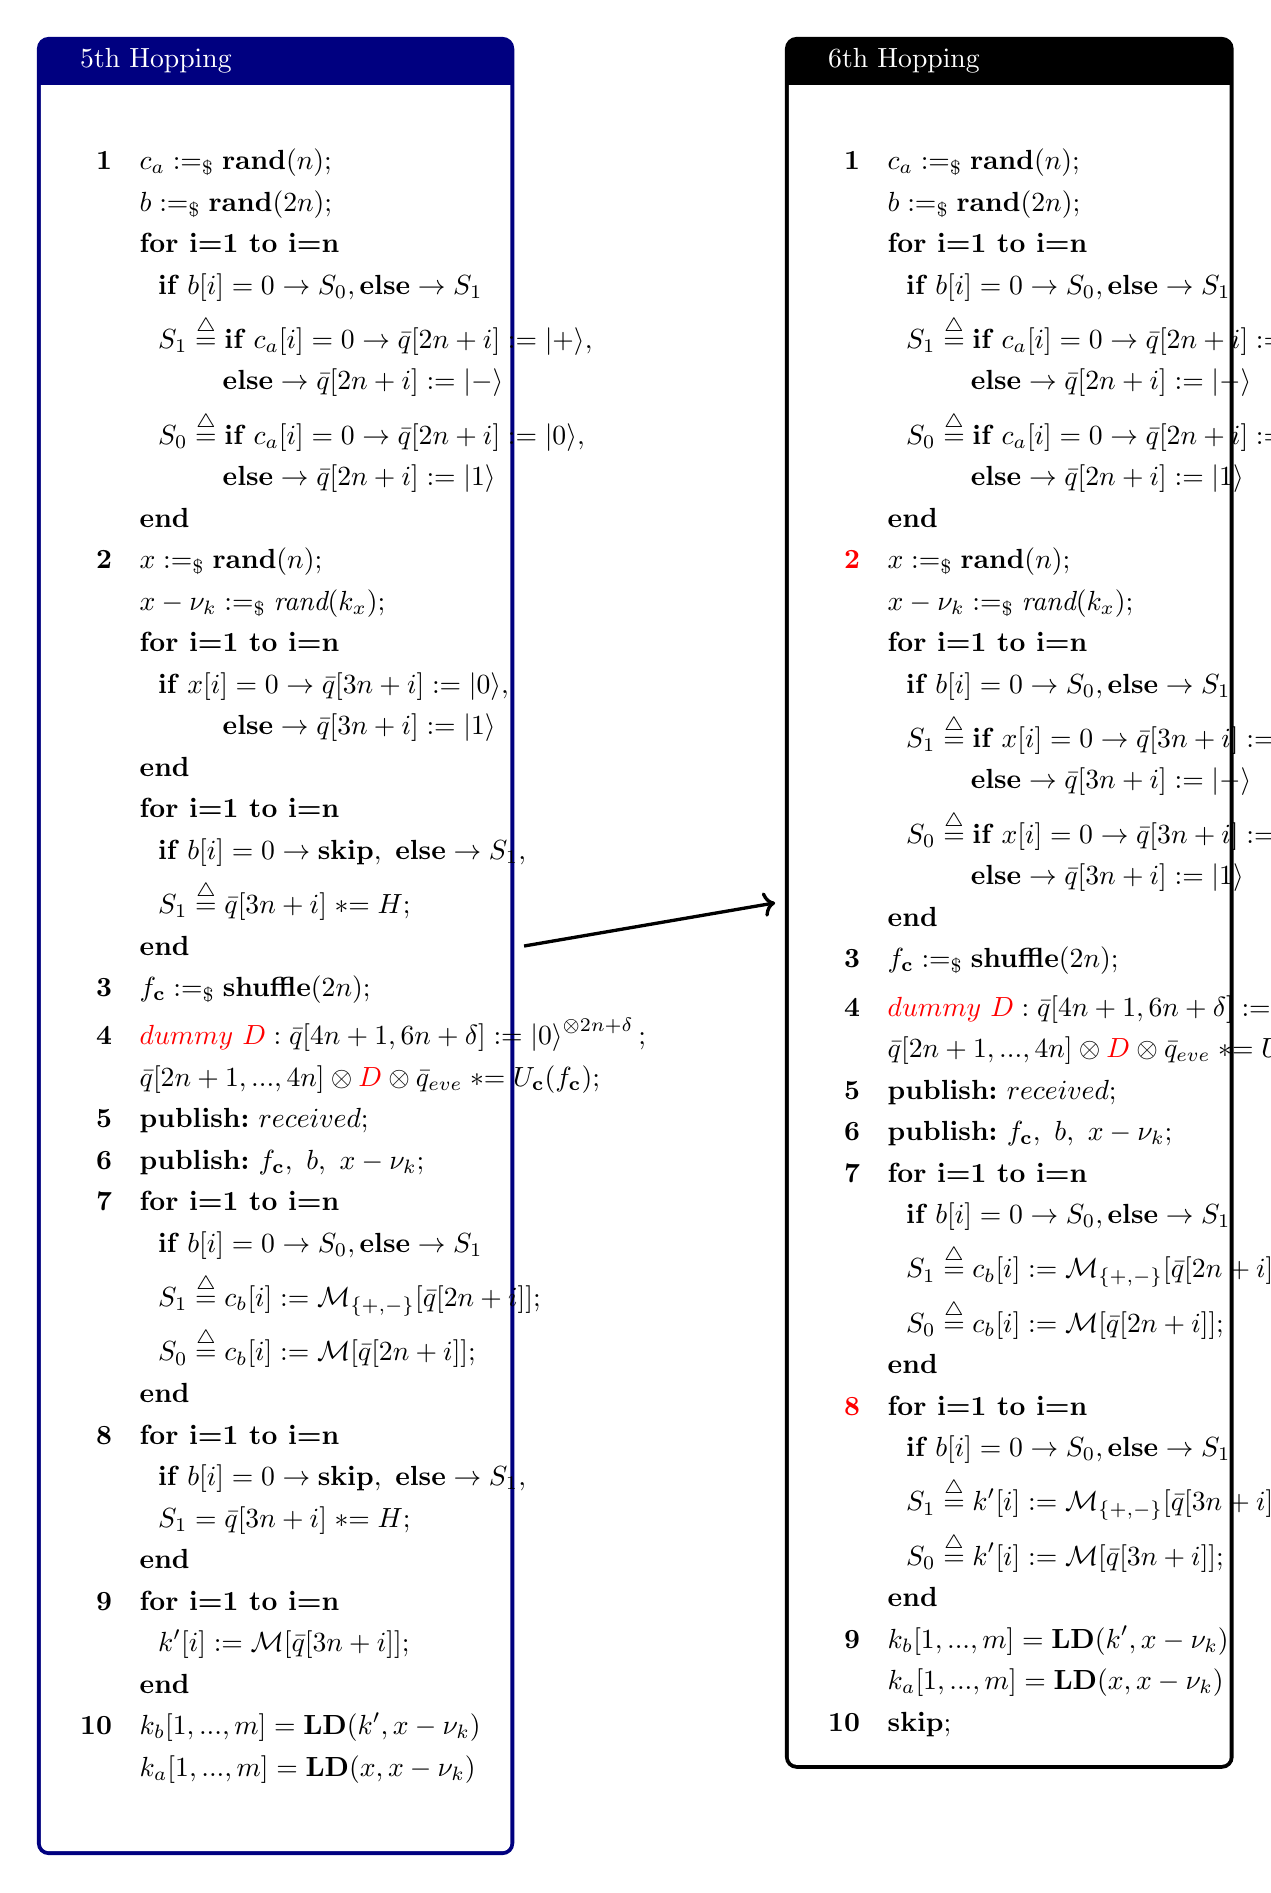
\begin{tikzpicture}[remember picture]

% Left box
\node[anchor=north west] (leftbox) at (0,0) {
\begin{minipage}[t]{0.5\textwidth}
\begin{tcolorbox}[colframe=blue!50!black, colback=white, title=5th Hopping, width=\textwidth]
\begin{align*}
    \textbf{{1}} \quad 
    & c_a :=_\$ \textbf{rand}(n); \\ 
    & b :=_\$ \textbf{rand}(2n); \\
    \quad 
    &\textbf{for i=1 to i=n}\\
    &~~ \textbf{if }  b[i] = 0 \rightarrow S_{0} ,\textbf{else}\rightarrow S_{1}\\
    &~~ S_{1}\stackrel{\triangle}{=}\textbf{if }  c_a[i] = 0 \rightarrow \bar{q}[2n+i] := |+\rangle,\\ &~~~~~~~~~\textbf{else}   \rightarrow \bar{q}[2n+i] := |-\rangle\\
    &~~ S_{0}\stackrel{\triangle}{=}\textbf{if }  c_a[i] = 0 \rightarrow \bar{q}[2n+i] := |0\rangle,\\ &~~~~~~~~~\textbf{else}   \rightarrow \bar{q}[2n+i] := |1\rangle\\
    &\textbf{end}\\
    \textbf{{2}}\quad 
    & x :=_\$ \textbf{rand}(n); \\
    & x-\nu_k :=_\$ \textit{rand}(k_x);\\
    &\textbf{for i=1 to i=n}\\
    &~~ \textbf{if }  x[i] = 0 \rightarrow \bar{q}[3n+i] := |0\rangle,\\ &~~~~~~~~~\textbf{else}   \rightarrow \bar{q}[3n+i] := |1\rangle\\
    &\textbf{end}\\
    &\textbf{for i=1 to i=n}\\
    &~~ \textbf{if }  b[i] = 0 \rightarrow \textbf{skip},~\textbf{else}\rightarrow S_{1} ,\\
    &~~ S_{1}\stackrel{\triangle}{=}\bar{q}[3n+i] \asteq H ;\\
    &\textbf{end}\\
    \textbf{{3}} \quad & f_{\textbf{c}}:=_\$\textbf{shuffle}(2n); \\
    \textbf{{4}} \quad & \textcolor{red}{dummy~D}: \bar{q}[4n+1,6n+\delta]:=\ket{0}^{\otimes 2n+\delta};\\     &\bar{q}[2n+1,...,4n]\otimes \textcolor{red}{D} \otimes \bar{q}_{eve} \asteq U_{\textbf{c}}(f_{\textbf{c}}); \\
    \textbf{{5}} \quad & \textbf{publish:}~ received;\\
    \textbf{{6}} \quad & \textbf{publish:}~ f_{\textbf{c}},~b,~x-\nu_k;\\
    \textbf{{7}} 
    \quad 
    &\textbf{for i=1 to i=n}\\
    &~~ \textbf{if }  b[i] = 0 \rightarrow S_{0} ,\textbf{else}\rightarrow S_{1}\\
    &~~ S_{1}\stackrel{\triangle}{=}c_b[i]:= \mathcal{M}_{\{+,-\}} [\bar{q}[2n+i]];\\
    &~~ S_{0}\stackrel{\triangle}{=}c_b[i]:= \mathcal{M} [\bar{q}[2n+i]];\\
    &\textbf{end}\\
    \textbf{{8}}\quad 
    &\textbf{for i=1 to i=n}\\
    &~~ \textbf{if }  b[i] = 0 \rightarrow \textbf{skip},~\textbf{else}\rightarrow S_{1} ,\\
    &~~ S_{1}=\bar{q}[3n+i] \asteq H ;\\
    &\textbf{end}\\
    \textbf{{9}} \quad 
    &\textbf{for i=1 to i=n}\\
    &~~ k'[i]:= \mathcal{M} [\bar{q}[3n+i]];\\
    &\textbf{end}\\
    {\textbf{10}} \quad & k_b[1,...,m]=\textbf{LD}(k',x-\nu_k)\\
    &k_a[1,...,m]=\textbf{LD}(x,x-\nu_k)\\
\end{align*}
\end{tcolorbox}
\end{minipage}
};

% Right box
\node[anchor=north west] (rightbox) at (9.5,0) {
\begin{minipage}[t]{0.47\textwidth}
\begin{tcolorbox}[colframe=black!50!black, colback=white, title=6th Hopping, width=\textwidth]
\begin{align*}
    \textbf{{1}} \quad 
    & c_a :=_\$ \textbf{rand}(n); \\ 
    & b :=_\$ \textbf{rand}(2n); \\
    \quad 
    &\textbf{for i=1 to i=n}\\
    &~~ \textbf{if }  b[i] = 0 \rightarrow S_{0} ,\textbf{else}\rightarrow S_{1}\\
    &~~ S_{1}\stackrel{\triangle}{=}\textbf{if }  c_a[i] = 0 \rightarrow \bar{q}[2n+i] := |+\rangle,\\ &~~~~~~~~~\textbf{else}   \rightarrow \bar{q}[2n+i] := |-\rangle\\
    &~~ S_{0}\stackrel{\triangle}{=}\textbf{if }  c_a[i] = 0 \rightarrow \bar{q}[2n+i] := |0\rangle,\\ &~~~~~~~~~\textbf{else}   \rightarrow \bar{q}[2n+i] := |1\rangle\\
    &\textbf{end}\\
    \textbf{\textcolor{red}{2}}\quad 
    & x :=_\$ \textbf{rand}(n); \\
    & x-\nu_k :=_\$ \textit{rand}(k_x);\\
    &\textbf{for i=1 to i=n}\\
    &~~ \textbf{if }  b[i] = 0 \rightarrow S_{0} ,\textbf{else}\rightarrow S_{1}\\
    &~~ S_{1}\stackrel{\triangle}{=}\textbf{if }  x[i] = 0 \rightarrow \bar{q}[3n+i] := |+\rangle,\\ &~~~~~~~~~\textbf{else}   \rightarrow \bar{q}[3n+i] := |-\rangle\\
    &~~ S_{0}\stackrel{\triangle}{=}\textbf{if }  x[i] = 0 \rightarrow \bar{q}[3n+i] := |0\rangle,\\ &~~~~~~~~~\textbf{else}   \rightarrow \bar{q}[3n+i] := |1\rangle\\
    &\textbf{end}\\
    \textbf{{3}} \quad & f_{\textbf{c}}:=_\$\textbf{shuffle}(2n); \\
    \textbf{{4}} \quad & \textcolor{red}{dummy~D}: \bar{q}[4n+1,6n+\delta]:=\ket{0}^{\otimes 2n+\delta};\\     &\bar{q}[2n+1,...,4n]\otimes \textcolor{red}{D} \otimes \bar{q}_{eve} \asteq U_{\textbf{c}}(f_{\textbf{c}}); \\
    \textbf{{5}} \quad & \textbf{publish:}~ received;\\
    \textbf{{6}} \quad & \textbf{publish:}~ f_{\textbf{c}},~b,~x-\nu_k;\\
    \textbf{{7}} 
    \quad 
    &\textbf{for i=1 to i=n}\\
    &~~ \textbf{if }  b[i] = 0 \rightarrow S_{0} ,\textbf{else}\rightarrow S_{1}\\
    &~~ S_{1}\stackrel{\triangle}{=}c_b[i]:= \mathcal{M}_{\{+,-\}} [\bar{q}[2n+i]];\\
    &~~ S_{0}\stackrel{\triangle}{=}c_b[i]:= \mathcal{M} [\bar{q}[2n+i]];\\
    &\textbf{end}\\
    \textbf{\textcolor{red}{8}}\quad 
    &\textbf{for i=1 to i=n}\\
    &~~ \textbf{if }  b[i] = 0 \rightarrow S_{0} ,\textbf{else}\rightarrow S_{1}\\
    &~~ S_{1}\stackrel{\triangle}{=}k'[i]:= \mathcal{M}_{\{+,-\}} [\bar{q}[3n+i]];\\
    &~~ S_{0}\stackrel{\triangle}{=}k'[i]:= \mathcal{M} [\bar{q}[3n+i]];\\
    &\textbf{end}\\
    \textbf{{9}} \quad 
    &k_b[1,...,m]=\textbf{LD}(k',x-\nu_k)\\
    &k_a[1,...,m]=\textbf{LD}(x,x-\nu_k)\\
    {\textbf{10}}\quad&\textbf{skip};
\end{align*}
\end{tcolorbox}
\end{minipage}
};

% Draw arrow between boxes
\draw[->, very thick] (leftbox.east) -- node[above]{} (rightbox.west);

\end{tikzpicture}
\newpage

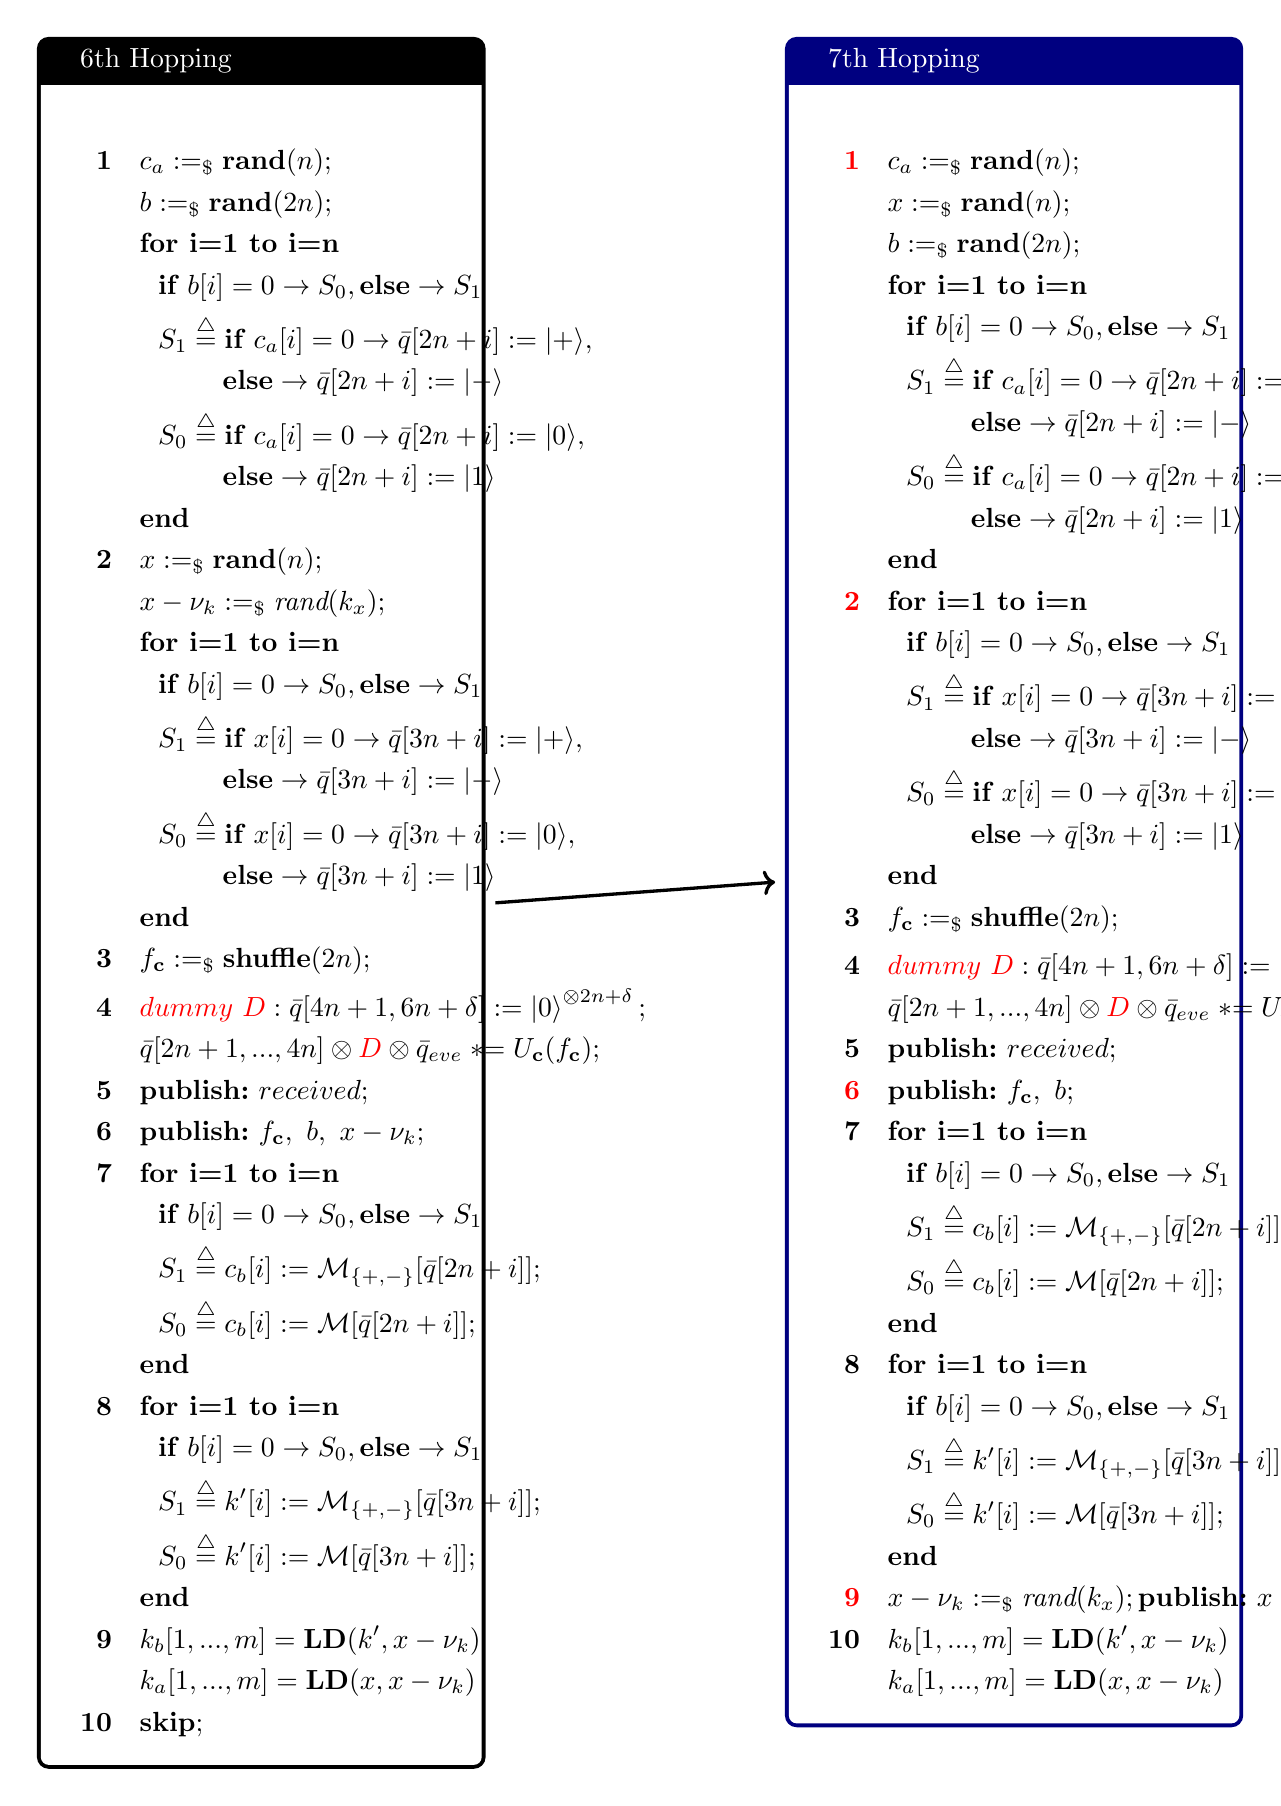
\begin{tikzpicture}[remember picture]

% Left box
\node[anchor=north west] (leftbox) at (0,0) {
\begin{minipage}[t]{0.47\textwidth}
\begin{tcolorbox}[colframe=black!50!black, colback=white, title=6th Hopping, width=\textwidth]
\begin{align*}
    \textbf{{1}} \quad 
    & c_a :=_\$ \textbf{rand}(n); \\ 
    & b :=_\$ \textbf{rand}(2n); \\
    \quad 
    &\textbf{for i=1 to i=n}\\
    &~~ \textbf{if }  b[i] = 0 \rightarrow S_{0} ,\textbf{else}\rightarrow S_{1}\\
    &~~ S_{1}\stackrel{\triangle}{=}\textbf{if }  c_a[i] = 0 \rightarrow \bar{q}[2n+i] := |+\rangle,\\ &~~~~~~~~~\textbf{else}   \rightarrow \bar{q}[2n+i] := |-\rangle\\
    &~~ S_{0}\stackrel{\triangle}{=}\textbf{if }  c_a[i] = 0 \rightarrow \bar{q}[2n+i] := |0\rangle,\\ &~~~~~~~~~\textbf{else}   \rightarrow \bar{q}[2n+i] := |1\rangle\\
    &\textbf{end}\\
    \textbf{{2}}\quad 
    & x :=_\$ \textbf{rand}(n); \\
    & x-\nu_k :=_\$ \textit{rand}(k_x);\\
    &\textbf{for i=1 to i=n}\\
    &~~ \textbf{if }  b[i] = 0 \rightarrow S_{0} ,\textbf{else}\rightarrow S_{1}\\
    &~~ S_{1}\stackrel{\triangle}{=}\textbf{if }  x[i] = 0 \rightarrow \bar{q}[3n+i] := |+\rangle,\\ &~~~~~~~~~\textbf{else}   \rightarrow \bar{q}[3n+i] := |-\rangle\\
    &~~ S_{0}\stackrel{\triangle}{=}\textbf{if }  x[i] = 0 \rightarrow \bar{q}[3n+i] := |0\rangle,\\ &~~~~~~~~~\textbf{else}   \rightarrow \bar{q}[3n+i] := |1\rangle\\
    &\textbf{end}\\
    \textbf{{3}} \quad & f_{\textbf{c}}:=_\$\textbf{shuffle}(2n); \\
    \textbf{{4}} \quad & \textcolor{red}{dummy~D}: \bar{q}[4n+1,6n+\delta]:=\ket{0}^{\otimes 2n+\delta};\\     &\bar{q}[2n+1,...,4n]\otimes \textcolor{red}{D} \otimes \bar{q}_{eve} \asteq U_{\textbf{c}}(f_{\textbf{c}}); \\
    \textbf{{5}} \quad & \textbf{publish:}~ received;\\
    \textbf{{6}} \quad & \textbf{publish:}~ f_{\textbf{c}},~b,~x-\nu_k;\\
    \textbf{{7}} 
    \quad 
    &\textbf{for i=1 to i=n}\\
    &~~ \textbf{if }  b[i] = 0 \rightarrow S_{0} ,\textbf{else}\rightarrow S_{1}\\
    &~~ S_{1}\stackrel{\triangle}{=}c_b[i]:= \mathcal{M}_{\{+,-\}} [\bar{q}[2n+i]];\\
    &~~ S_{0}\stackrel{\triangle}{=}c_b[i]:= \mathcal{M} [\bar{q}[2n+i]];\\
    &\textbf{end}\\
    \textbf{{8}}\quad 
    &\textbf{for i=1 to i=n}\\
    &~~ \textbf{if }  b[i] = 0 \rightarrow S_{0} ,\textbf{else}\rightarrow S_{1}\\
    &~~ S_{1}\stackrel{\triangle}{=}k'[i]:= \mathcal{M}_{\{+,-\}} [\bar{q}[3n+i]];\\
    &~~ S_{0}\stackrel{\triangle}{=}k'[i]:= \mathcal{M} [\bar{q}[3n+i]];\\
    &\textbf{end}\\
    \textbf{{9}} \quad 
    &k_b[1,...,m]=\textbf{LD}(k',x-\nu_k)\\
    &k_a[1,...,m]=\textbf{LD}(x,x-\nu_k)\\
    {\textbf{10}}\quad&\textbf{skip};
\end{align*}
\end{tcolorbox}
\end{minipage}
};

% Right box
\node[anchor=north west] (rightbox) at (9.5,0) {
\begin{minipage}[t]{0.48\textwidth}
\begin{tcolorbox}[colframe=blue!50!black, colback=white, title=7th Hopping, width=\textwidth]
\begin{align*}
    \textbf{\textcolor{red}{1}} \quad 
    & c_a :=_\$ \textbf{rand}(n); \\ 
    & x :=_\$ \textbf{rand}(n); \\ 
    & b :=_\$ \textbf{rand}(2n); \\
    \quad 
    &\textbf{for i=1 to i=n}\\
    &~~ \textbf{if }  b[i] = 0 \rightarrow S_{0} ,\textbf{else}\rightarrow S_{1}\\
    &~~ S_{1}\stackrel{\triangle}{=}\textbf{if }  c_a[i] = 0 \rightarrow \bar{q}[2n+i] := |+\rangle,\\ &~~~~~~~~~\textbf{else}   \rightarrow \bar{q}[2n+i] := |-\rangle\\
    &~~ S_{0}\stackrel{\triangle}{=}\textbf{if }  c_a[i] = 0 \rightarrow \bar{q}[2n+i] := |0\rangle,\\ &~~~~~~~~~\textbf{else}   \rightarrow \bar{q}[2n+i] := |1\rangle\\
    &\textbf{end}\\
    \textbf{\textcolor{red}{2}}\quad 
    &\textbf{for i=1 to i=n}\\
    &~~ \textbf{if }  b[i] = 0 \rightarrow S_{0} ,\textbf{else}\rightarrow S_{1}\\
    &~~ S_{1}\stackrel{\triangle}{=}\textbf{if }  x[i] = 0 \rightarrow \bar{q}[3n+i] := |+\rangle,\\ &~~~~~~~~~\textbf{else}   \rightarrow \bar{q}[3n+i] := |-\rangle\\
    &~~ S_{0}\stackrel{\triangle}{=}\textbf{if }  x[i] = 0 \rightarrow \bar{q}[3n+i] := |0\rangle,\\ &~~~~~~~~~\textbf{else}   \rightarrow \bar{q}[3n+i] := |1\rangle\\
    &\textbf{end}\\
    \textbf{{3}} \quad & f_{\textbf{c}}:=_\$\textbf{shuffle}(2n); \\
    \textbf{{4}} \quad & \textcolor{red}{dummy~D}: \bar{q}[4n+1,6n+\delta]:=\ket{0}^{\otimes 2n+\delta};\\     &\bar{q}[2n+1,...,4n]\otimes \textcolor{red}{D} \otimes \bar{q}_{eve} \asteq U_{\textbf{c}}(f_{\textbf{c}}); \\
    \textbf{{5}} \quad & \textbf{publish:}~ received;\\
    \textbf{\textcolor{red}{6}} \quad & \textbf{publish:}~ f_{\textbf{c}},~b;\\
    \textbf{{7}} 
    \quad 
    &\textbf{for i=1 to i=n}\\
    &~~ \textbf{if }  b[i] = 0 \rightarrow S_{0} ,\textbf{else}\rightarrow S_{1}\\
    &~~ S_{1}\stackrel{\triangle}{=}c_b[i]:= \mathcal{M}_{\{+,-\}} [\bar{q}[2n+i]];\\
    &~~ S_{0}\stackrel{\triangle}{=}c_b[i]:= \mathcal{M} [\bar{q}[2n+i]];\\
    &\textbf{end}\\
    \textbf{{8}}\quad 
    &\textbf{for i=1 to i=n}\\
    &~~ \textbf{if }  b[i] = 0 \rightarrow S_{0} ,\textbf{else}\rightarrow S_{1}\\
    &~~ S_{1}\stackrel{\triangle}{=}k'[i]:= \mathcal{M}_{\{+,-\}} [\bar{q}[3n+i]];\\
    &~~ S_{0}\stackrel{\triangle}{=}k'[i]:= \mathcal{M} [\bar{q}[3n+i]];\\
    &\textbf{end}\\
    \textbf{\textcolor{red}{9}} \quad & x-\nu_k :=_\$ \textit{rand}(k_x); \textbf{publish:}~ x-\nu_k;\\
    \textbf{{10}} \quad 
    &k_b[1,...,m]=\textbf{LD}(k',x-\nu_k)\\
    &k_a[1,...,m]=\textbf{LD}(x,x-\nu_k)
\end{align*}
\end{tcolorbox}
\end{minipage}
};

% Draw arrow between boxes
\draw[->, very thick] (leftbox.east) -- node[above]{} (rightbox.west);

\end{tikzpicture}
\newpage

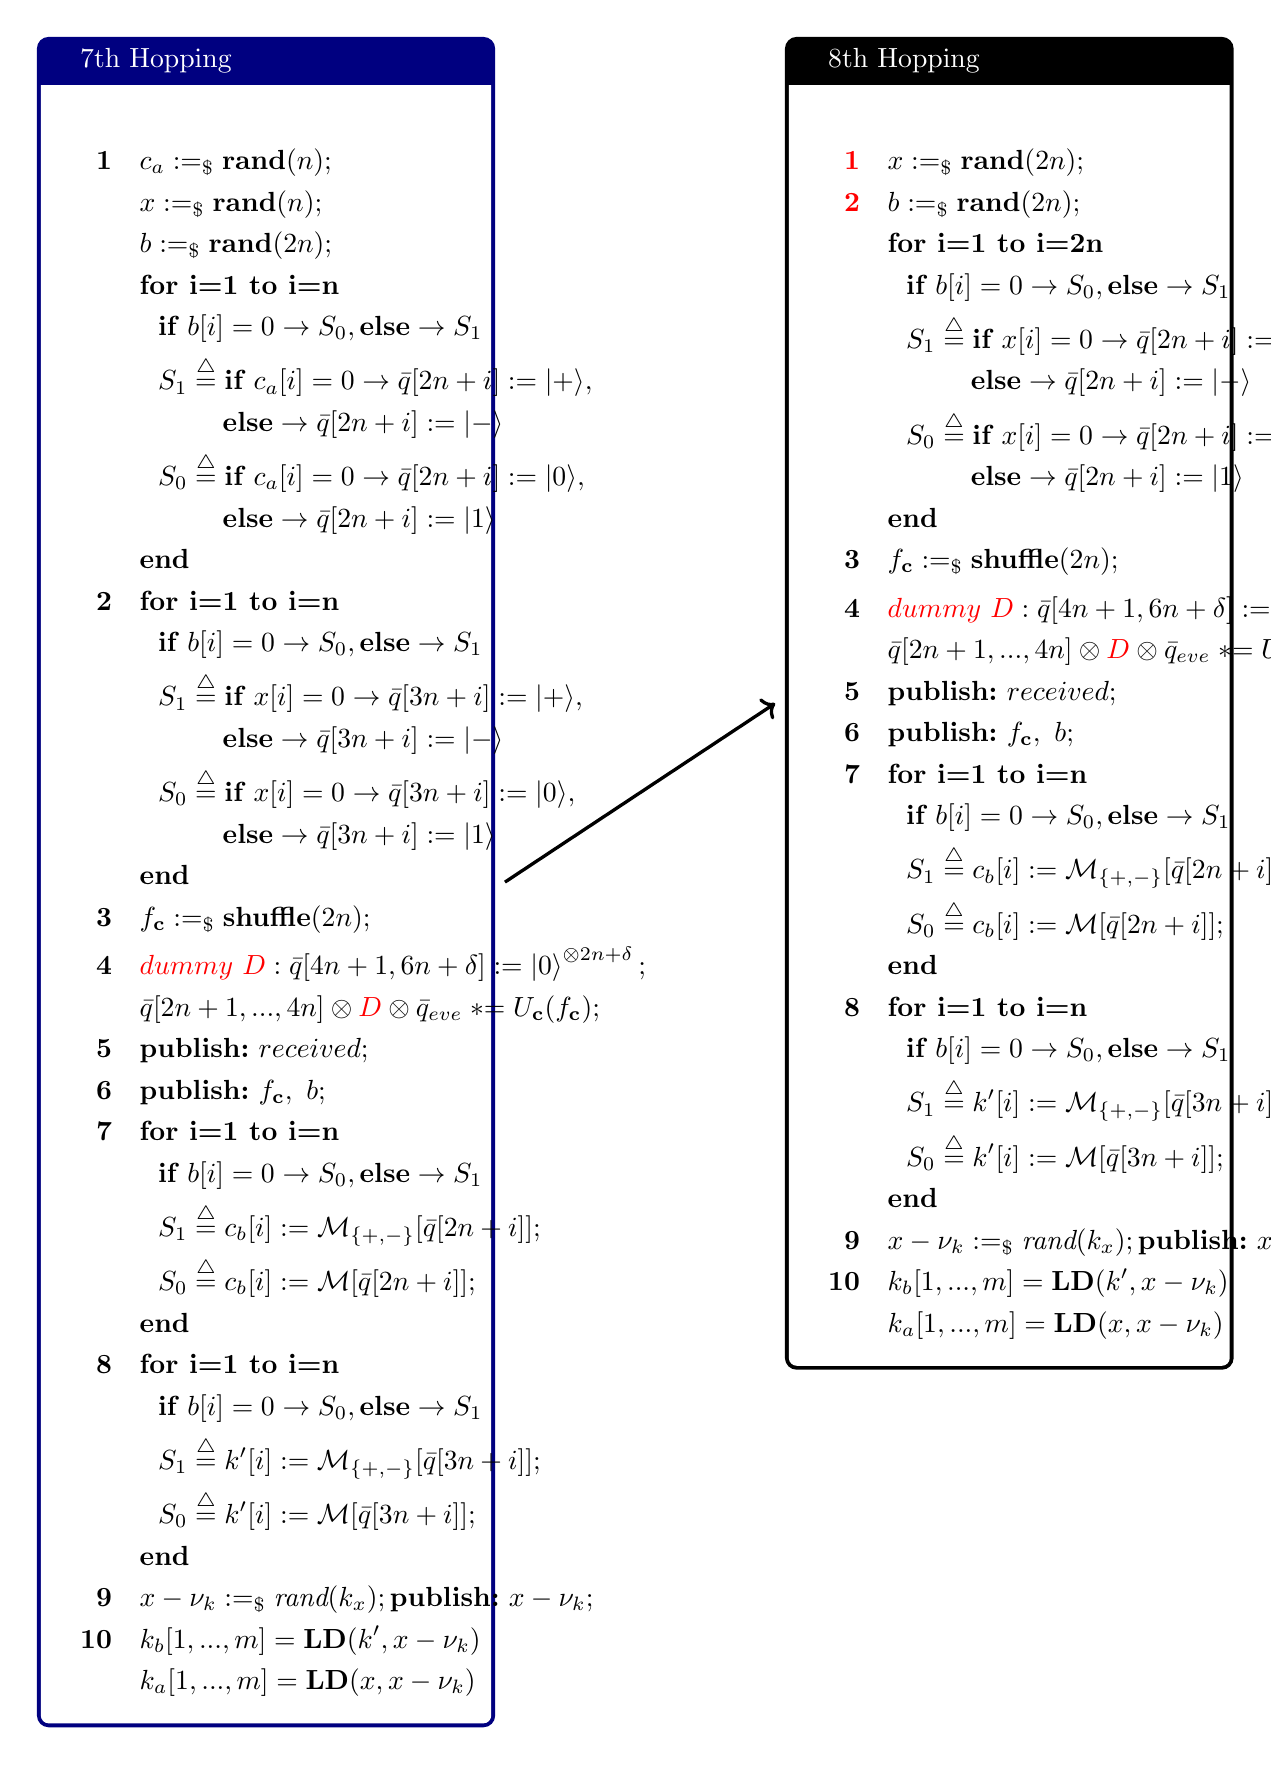
\begin{tikzpicture}[remember picture]

% Left box
\node[anchor=north west] (leftbox) at (0,0) {
\begin{minipage}[t]{0.48\textwidth}
\begin{tcolorbox}[colframe=blue!50!black, colback=white, title=7th Hopping, width=\textwidth]
\begin{align*}
    \textbf{{1}} \quad 
    & c_a :=_\$ \textbf{rand}(n); \\ 
    & x :=_\$ \textbf{rand}(n); \\ 
    & b :=_\$ \textbf{rand}(2n); \\
    \quad 
    &\textbf{for i=1 to i=n}\\
    &~~ \textbf{if }  b[i] = 0 \rightarrow S_{0} ,\textbf{else}\rightarrow S_{1}\\
    &~~ S_{1}\stackrel{\triangle}{=}\textbf{if }  c_a[i] = 0 \rightarrow \bar{q}[2n+i] := |+\rangle,\\ &~~~~~~~~~\textbf{else}   \rightarrow \bar{q}[2n+i] := |-\rangle\\
    &~~ S_{0}\stackrel{\triangle}{=}\textbf{if }  c_a[i] = 0 \rightarrow \bar{q}[2n+i] := |0\rangle,\\ &~~~~~~~~~\textbf{else}   \rightarrow \bar{q}[2n+i] := |1\rangle\\
    &\textbf{end}\\
    \textbf{{2}}\quad 
    &\textbf{for i=1 to i=n}\\
    &~~ \textbf{if }  b[i] = 0 \rightarrow S_{0} ,\textbf{else}\rightarrow S_{1}\\
    &~~ S_{1}\stackrel{\triangle}{=}\textbf{if }  x[i] = 0 \rightarrow \bar{q}[3n+i] := |+\rangle,\\ &~~~~~~~~~\textbf{else}   \rightarrow \bar{q}[3n+i] := |-\rangle\\
    &~~ S_{0}\stackrel{\triangle}{=}\textbf{if }  x[i] = 0 \rightarrow \bar{q}[3n+i] := |0\rangle,\\ &~~~~~~~~~\textbf{else}   \rightarrow \bar{q}[3n+i] := |1\rangle\\
    &\textbf{end}\\
    \textbf{{3}} \quad & f_{\textbf{c}}:=_\$\textbf{shuffle}(2n); \\
    \textbf{{4}} \quad & \textcolor{red}{dummy~D}: \bar{q}[4n+1,6n+\delta]:=\ket{0}^{\otimes 2n+\delta};\\     &\bar{q}[2n+1,...,4n]\otimes \textcolor{red}{D} \otimes \bar{q}_{eve} \asteq U_{\textbf{c}}(f_{\textbf{c}}); \\
    \textbf{{5}} \quad & \textbf{publish:}~ received;\\
    \textbf{{6}} \quad & \textbf{publish:}~ f_{\textbf{c}},~b;\\
    \textbf{{7}} 
    \quad 
    &\textbf{for i=1 to i=n}\\
    &~~ \textbf{if }  b[i] = 0 \rightarrow S_{0} ,\textbf{else}\rightarrow S_{1}\\
    &~~ S_{1}\stackrel{\triangle}{=}c_b[i]:= \mathcal{M}_{\{+,-\}} [\bar{q}[2n+i]];\\
    &~~ S_{0}\stackrel{\triangle}{=}c_b[i]:= \mathcal{M} [\bar{q}[2n+i]];\\
    &\textbf{end}\\
    \textbf{{8}}\quad 
    &\textbf{for i=1 to i=n}\\
    &~~ \textbf{if }  b[i] = 0 \rightarrow S_{0} ,\textbf{else}\rightarrow S_{1}\\
    &~~ S_{1}\stackrel{\triangle}{=}k'[i]:= \mathcal{M}_{\{+,-\}} [\bar{q}[3n+i]];\\
    &~~ S_{0}\stackrel{\triangle}{=}k'[i]:= \mathcal{M} [\bar{q}[3n+i]];\\
    &\textbf{end}\\
    \textbf{{9}} \quad & x-\nu_k :=_\$ \textit{rand}(k_x); \textbf{publish:}~ x-\nu_k;\\
    \textbf{{10}} \quad 
    &k_b[1,...,m]=\textbf{LD}(k',x-\nu_k)\\
    &k_a[1,...,m]=\textbf{LD}(x,x-\nu_k)
\end{align*}
\end{tcolorbox}
\end{minipage}
};

% Right box
\node[anchor=north west] (rightbox) at (9.5,0) {
\begin{minipage}[t]{0.47\textwidth}
\begin{tcolorbox}[colframe=black!50!black, colback=white, title=8th Hopping, width=\textwidth]
\begin{align*}
    \textbf{\textcolor{red}{1}} \quad 
    & x :=_\$ \textbf{rand}(2n); \\ 
    \textbf{\textcolor{red}{2}}\quad 
    & b :=_\$ \textbf{rand}(2n); \\
    &\textbf{for i=1 to i=2n}\\
    &~~ \textbf{if }  b[i] = 0 \rightarrow S_{0} ,\textbf{else}\rightarrow S_{1}\\
    &~~ S_{1}\stackrel{\triangle}{=}\textbf{if }  x[i] = 0 \rightarrow \bar{q}[2n+i] := |+\rangle,\\ &~~~~~~~~~\textbf{else}   \rightarrow \bar{q}[2n+i] := |-\rangle\\
    &~~ S_{0}\stackrel{\triangle}{=}\textbf{if }  x[i] = 0 \rightarrow \bar{q}[2n+i] := |0\rangle,\\ &~~~~~~~~~\textbf{else}   \rightarrow \bar{q}[2n+i] := |1\rangle\\
    &\textbf{end}\\
    \textbf{{3}} \quad & f_{\textbf{c}}:=_\$\textbf{shuffle}(2n); \\
    \textbf{{4}} \quad & \textcolor{red}{dummy~D}: \bar{q}[4n+1,6n+\delta]:=\ket{0}^{\otimes 2n+\delta};\\     &\bar{q}[2n+1,...,4n]\otimes \textcolor{red}{D} \otimes \bar{q}_{eve} \asteq U_{\textbf{c}}(f_{\textbf{c}}); \\
    \textbf{{5}} \quad & \textbf{publish:}~ received;\\
    \textbf{{6}} \quad & \textbf{publish:}~ f_{\textbf{c}},~b;\\
    \textbf{{7}} 
    \quad 
    &\textbf{for i=1 to i=n}\\
    &~~ \textbf{if }  b[i] = 0 \rightarrow S_{0} ,\textbf{else}\rightarrow S_{1}\\
    &~~ S_{1}\stackrel{\triangle}{=}c_b[i]:= \mathcal{M}_{\{+,-\}} [\bar{q}[2n+i]];\\
    &~~ S_{0}\stackrel{\triangle}{=}c_b[i]:= \mathcal{M} [\bar{q}[2n+i]];\\
    &\textbf{end}\\
    \textbf{{8}}\quad 
    &\textbf{for i=1 to i=n}\\
    &~~ \textbf{if }  b[i] = 0 \rightarrow S_{0} ,\textbf{else}\rightarrow S_{1}\\
    &~~ S_{1}\stackrel{\triangle}{=}k'[i]:= \mathcal{M}_{\{+,-\}} [\bar{q}[3n+i]];\\
    &~~ S_{0}\stackrel{\triangle}{=}k'[i]:= \mathcal{M} [\bar{q}[3n+i]];\\
    &\textbf{end}\\
    \textbf{{9}} \quad & x-\nu_k :=_\$ \textit{rand}(k_x); \textbf{publish:}~ x-\nu_k;\\
    \textbf{{10}} \quad 
    &k_b[1,...,m]=\textbf{LD}(k',x-\nu_k)\\
    &k_a[1,...,m]=\textbf{LD}(x,x-\nu_k)
\end{align*}
\end{tcolorbox}
\end{minipage}
};

% Draw arrow between boxes
\draw[->, very thick] (leftbox.east) -- node[above]{} (rightbox.west);

\end{tikzpicture}
\newpage

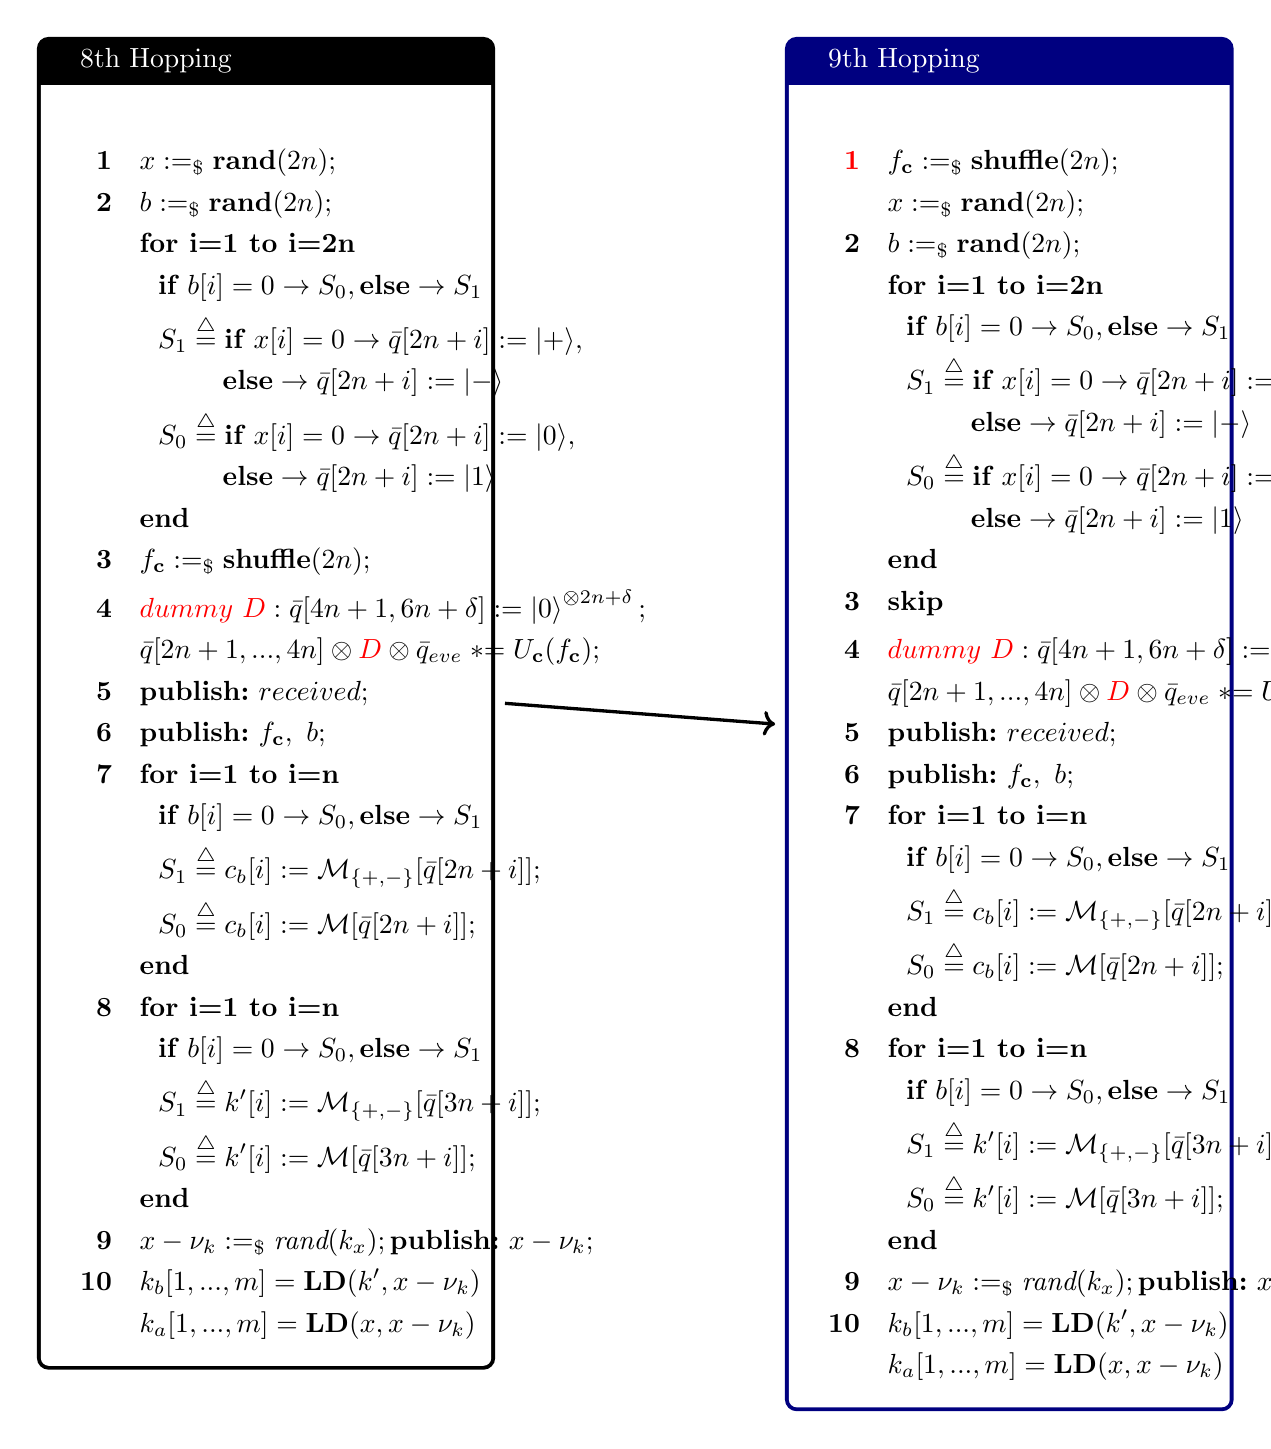
\begin{tikzpicture}[remember picture]

% Left box
\node[anchor=north west] (leftbox) at (0,0) {
\begin{minipage}[t]{0.48\textwidth}
\begin{tcolorbox}[colframe=black!50!black, colback=white, title=8th Hopping, width=\textwidth]
\begin{align*}
    \textbf{{1}} \quad 
    & x :=_\$ \textbf{rand}(2n); \\ 
    \textbf{{2}}\quad 
    & b :=_\$ \textbf{rand}(2n); \\
    &\textbf{for i=1 to i=2n}\\
    &~~ \textbf{if }  b[i] = 0 \rightarrow S_{0} ,\textbf{else}\rightarrow S_{1}\\
    &~~ S_{1}\stackrel{\triangle}{=}\textbf{if }  x[i] = 0 \rightarrow \bar{q}[2n+i] := |+\rangle,\\ &~~~~~~~~~\textbf{else}   \rightarrow \bar{q}[2n+i] := |-\rangle\\
    &~~ S_{0}\stackrel{\triangle}{=}\textbf{if }  x[i] = 0 \rightarrow \bar{q}[2n+i] := |0\rangle,\\ &~~~~~~~~~\textbf{else}   \rightarrow \bar{q}[2n+i] := |1\rangle\\
    &\textbf{end}\\
    \textbf{{3}} \quad & f_{\textbf{c}}:=_\$\textbf{shuffle}(2n); \\
    \textbf{{4}} \quad & \textcolor{red}{dummy~D}: \bar{q}[4n+1,6n+\delta]:=\ket{0}^{\otimes 2n+\delta};\\     &\bar{q}[2n+1,...,4n]\otimes \textcolor{red}{D} \otimes \bar{q}_{eve} \asteq U_{\textbf{c}}(f_{\textbf{c}}); \\
    \textbf{{5}} \quad & \textbf{publish:}~ received;\\
    \textbf{{6}} \quad & \textbf{publish:}~ f_{\textbf{c}},~b;\\
    \textbf{{7}} 
    \quad 
    &\textbf{for i=1 to i=n}\\
    &~~ \textbf{if }  b[i] = 0 \rightarrow S_{0} ,\textbf{else}\rightarrow S_{1}\\
    &~~ S_{1}\stackrel{\triangle}{=}c_b[i]:= \mathcal{M}_{\{+,-\}} [\bar{q}[2n+i]];\\
    &~~ S_{0}\stackrel{\triangle}{=}c_b[i]:= \mathcal{M} [\bar{q}[2n+i]];\\
    &\textbf{end}\\
    \textbf{{8}}\quad 
    &\textbf{for i=1 to i=n}\\
    &~~ \textbf{if }  b[i] = 0 \rightarrow S_{0} ,\textbf{else}\rightarrow S_{1}\\
    &~~ S_{1}\stackrel{\triangle}{=}k'[i]:= \mathcal{M}_{\{+,-\}} [\bar{q}[3n+i]];\\
    &~~ S_{0}\stackrel{\triangle}{=}k'[i]:= \mathcal{M} [\bar{q}[3n+i]];\\
    &\textbf{end}\\
    \textbf{{9}} \quad & x-\nu_k :=_\$ \textit{rand}(k_x); \textbf{publish:}~ x-\nu_k;\\
    \textbf{{10}} \quad 
    &k_b[1,...,m]=\textbf{LD}(k',x-\nu_k)\\
    &k_a[1,...,m]=\textbf{LD}(x,x-\nu_k)
\end{align*}
\end{tcolorbox}
\end{minipage}
};

% Right box
\node[anchor=north west] (rightbox) at (9.5,0) {
\begin{minipage}[t]{0.47\textwidth}
\begin{tcolorbox}[colframe=blue!50!black, colback=white, title=9th Hopping, width=\textwidth]
\begin{align*}
    \textbf{\textcolor{red}{1}} \quad 
    &f_{\textbf{c}}:=_\$\textbf{shuffle}(2n); \\
    &x :=_\$ \textbf{rand}(2n); \\ 
    \textbf{{2}}\quad 
    & b :=_\$ \textbf{rand}(2n); \\
    &\textbf{for i=1 to i=2n}\\
    &~~ \textbf{if }  b[i] = 0 \rightarrow S_{0} ,\textbf{else}\rightarrow S_{1}\\
    &~~ S_{1}\stackrel{\triangle}{=}\textbf{if }  x[i] = 0 \rightarrow \bar{q}[2n+i] := |+\rangle,\\ &~~~~~~~~~\textbf{else}   \rightarrow \bar{q}[2n+i] := |-\rangle\\
    &~~ S_{0}\stackrel{\triangle}{=}\textbf{if }  x[i] = 0 \rightarrow \bar{q}[2n+i] := |0\rangle,\\ &~~~~~~~~~\textbf{else}   \rightarrow \bar{q}[2n+i] := |1\rangle\\
    &\textbf{end}\\
    \textbf{{3}} \quad & \textbf{skip}\\
    \textbf{{4}} \quad & \textcolor{red}{dummy~D}: \bar{q}[4n+1,6n+\delta]:=\ket{0}^{\otimes 2n+\delta};\\     &\bar{q}[2n+1,...,4n]\otimes \textcolor{red}{D} \otimes \bar{q}_{eve} \asteq U_{\textbf{c}}(f_{\textbf{c}}); \\
    \textbf{{5}} \quad & \textbf{publish:}~ received;\\
    \textbf{{6}} \quad & \textbf{publish:}~ f_{\textbf{c}},~b;\\
    \textbf{{7}} 
    \quad 
    &\textbf{for i=1 to i=n}\\
    &~~ \textbf{if }  b[i] = 0 \rightarrow S_{0} ,\textbf{else}\rightarrow S_{1}\\
    &~~ S_{1}\stackrel{\triangle}{=}c_b[i]:= \mathcal{M}_{\{+,-\}} [\bar{q}[2n+i]];\\
    &~~ S_{0}\stackrel{\triangle}{=}c_b[i]:= \mathcal{M} [\bar{q}[2n+i]];\\
    &\textbf{end}\\
    \textbf{{8}}\quad 
    &\textbf{for i=1 to i=n}\\
    &~~ \textbf{if }  b[i] = 0 \rightarrow S_{0} ,\textbf{else}\rightarrow S_{1}\\
    &~~ S_{1}\stackrel{\triangle}{=}k'[i]:= \mathcal{M}_{\{+,-\}} [\bar{q}[3n+i]];\\
    &~~ S_{0}\stackrel{\triangle}{=}k'[i]:= \mathcal{M} [\bar{q}[3n+i]];\\
    &\textbf{end}\\
    \textbf{{9}} \quad & x-\nu_k :=_\$ \textit{rand}(k_x); \textbf{publish:}~ x-\nu_k;\\
    \textbf{{10}} \quad 
    &k_b[1,...,m]=\textbf{LD}(k',x-\nu_k)\\
    &k_a[1,...,m]=\textbf{LD}(x,x-\nu_k)
\end{align*}
\end{tcolorbox}
\end{minipage}
};

% Draw arrow between boxes
\draw[->, very thick] (leftbox.east) -- node[above]{} (rightbox.west);

\end{tikzpicture}

\newpage


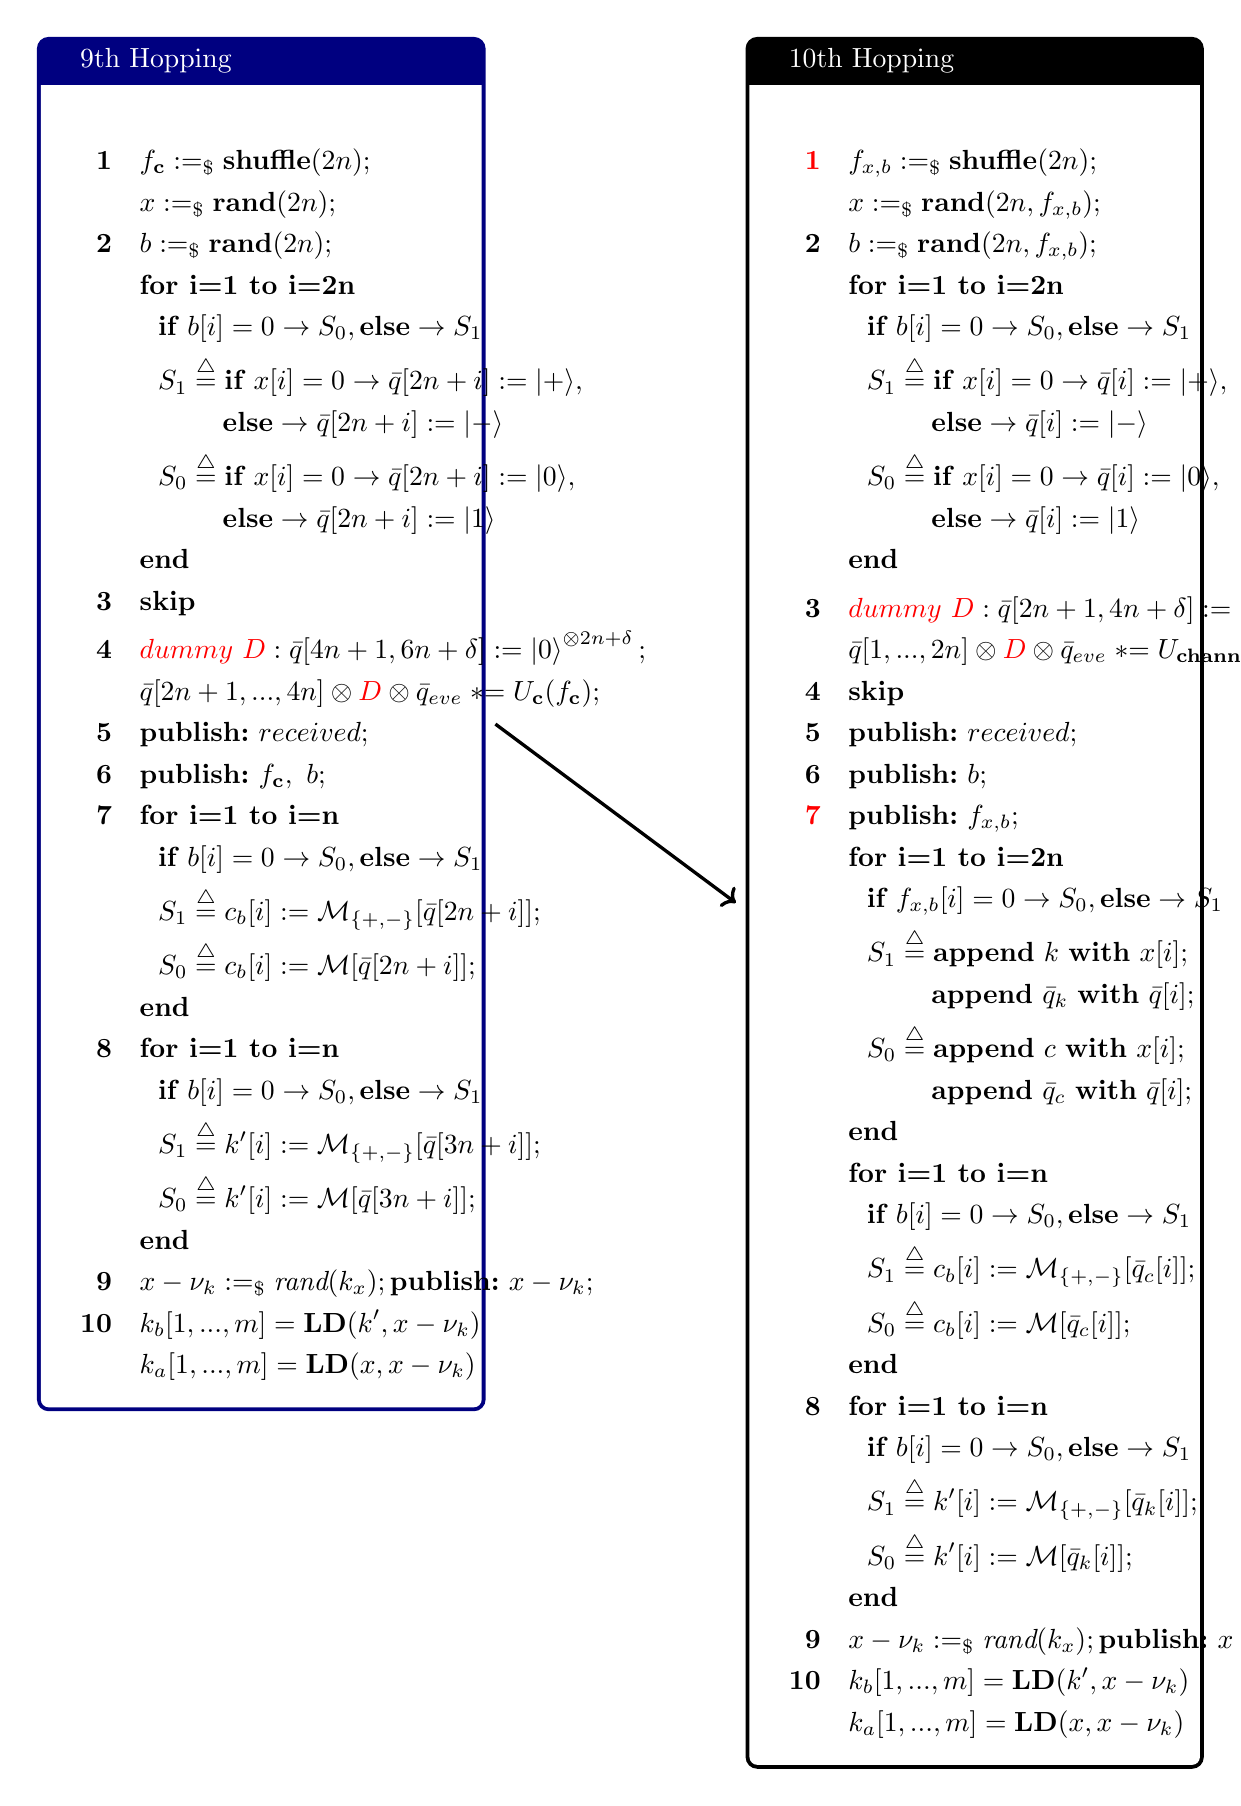
\begin{tikzpicture}[remember picture]

% Left box
\node[anchor=north west] (leftbox) at (0,0) {
\begin{minipage}[t]{0.47\textwidth}
\begin{tcolorbox}[colframe=blue!50!black, colback=white, title=9th Hopping, width=\textwidth]
\begin{align*}
    \textbf{{1}} \quad 
    &f_{\textbf{c}}:=_\$\textbf{shuffle}(2n); \\
    &x :=_\$ \textbf{rand}(2n); \\ 
    \textbf{{2}}\quad 
    & b :=_\$ \textbf{rand}(2n); \\
    &\textbf{for i=1 to i=2n}\\
    &~~ \textbf{if }  b[i] = 0 \rightarrow S_{0} ,\textbf{else}\rightarrow S_{1}\\
    &~~ S_{1}\stackrel{\triangle}{=}\textbf{if }  x[i] = 0 \rightarrow \bar{q}[2n+i] := |+\rangle,\\ &~~~~~~~~~\textbf{else}   \rightarrow \bar{q}[2n+i] := |-\rangle\\
    &~~ S_{0}\stackrel{\triangle}{=}\textbf{if }  x[i] = 0 \rightarrow \bar{q}[2n+i] := |0\rangle,\\ &~~~~~~~~~\textbf{else}   \rightarrow \bar{q}[2n+i] := |1\rangle\\
    &\textbf{end}\\
    \textbf{{3}} \quad & \textbf{skip}\\
    \textbf{{4}} \quad & \textcolor{red}{dummy~D}: \bar{q}[4n+1,6n+\delta]:=\ket{0}^{\otimes 2n+\delta};\\     &\bar{q}[2n+1,...,4n]\otimes \textcolor{red}{D} \otimes \bar{q}_{eve} \asteq U_{\textbf{c}}(f_{\textbf{c}}); \\
    \textbf{{5}} \quad & \textbf{publish:}~ received;\\
    \textbf{{6}} \quad & \textbf{publish:}~ f_{\textbf{c}},~b;\\
    \textbf{{7}} 
    \quad 
    &\textbf{for i=1 to i=n}\\
    &~~ \textbf{if }  b[i] = 0 \rightarrow S_{0} ,\textbf{else}\rightarrow S_{1}\\
    &~~ S_{1}\stackrel{\triangle}{=}c_b[i]:= \mathcal{M}_{\{+,-\}} [\bar{q}[2n+i]];\\
    &~~ S_{0}\stackrel{\triangle}{=}c_b[i]:= \mathcal{M} [\bar{q}[2n+i]];\\
    &\textbf{end}\\
    \textbf{{8}}\quad 
    &\textbf{for i=1 to i=n}\\
    &~~ \textbf{if }  b[i] = 0 \rightarrow S_{0} ,\textbf{else}\rightarrow S_{1}\\
    &~~ S_{1}\stackrel{\triangle}{=}k'[i]:= \mathcal{M}_{\{+,-\}} [\bar{q}[3n+i]];\\
    &~~ S_{0}\stackrel{\triangle}{=}k'[i]:= \mathcal{M} [\bar{q}[3n+i]];\\
    &\textbf{end}\\
    \textbf{{9}} \quad & x-\nu_k :=_\$ \textit{rand}(k_x); \textbf{publish:}~ x-\nu_k;\\
    \textbf{{10}} \quad 
    &k_b[1,...,m]=\textbf{LD}(k',x-\nu_k)\\
    &k_a[1,...,m]=\textbf{LD}(x,x-\nu_k)
\end{align*}
\end{tcolorbox}
\end{minipage}
};

% Right box
\node[anchor=north west] (rightbox) at (9,0) {
\begin{minipage}[t]{0.48\textwidth}
\begin{tcolorbox}[colframe=black!50!black, colback=white, title=10th Hopping, width=\textwidth]
\begin{align*}
    \textbf{\textcolor{red}{1}} \quad 
    & f_{x,b}:=_\$\textbf{shuffle}(2n); \\
    &x :=_\$ \textbf{rand}(2n,f_{x,b}); \\ 
    \textbf{{2}}\quad 
    & b :=_\$ \textbf{rand}(2n,f_{x,b}); \\
    &\textbf{for i=1 to i=2n}\\
    &~~ \textbf{if }  b[i] = 0 \rightarrow S_{0} ,\textbf{else}\rightarrow S_{1}\\
    &~~ S_{1}\stackrel{\triangle}{=}\textbf{if }  x[i] = 0 \rightarrow \bar{q}[i] := |+\rangle,\\ &~~~~~~~~~\textbf{else}   \rightarrow \bar{q}[i] := |-\rangle\\
    &~~ S_{0}\stackrel{\triangle}{=}\textbf{if }  x[i] = 0 \rightarrow \bar{q}[i] := |0\rangle,\\ &~~~~~~~~~\textbf{else}   \rightarrow \bar{q}[i] := |1\rangle\\
    &\textbf{end}\\
    \textbf{{3}} 
    \quad & \textcolor{red}{dummy~D}: \bar{q}[2n+1,4n+\delta]:=\ket{0}^{\otimes 2n+\delta};\\     &\bar{q}[1,...,2n]\otimes \textcolor{red}{D} \otimes \bar{q}_{eve} \asteq U_{\textbf{channel seq}}; \\
    \textbf{{4}} \quad &\textbf{skip} \\ 
    \textbf{{5}} \quad & \textbf{publish:}~ received;\\
    \textbf{{6}} \quad & \textbf{publish:}~b;\\
    \textbf{\textcolor{red}{7}} 
    \quad & \textbf{publish:}~ f_{x,b};\\
    &\textbf{for i=1  to i=2n}\\
    &~~ \textbf{if }  f_{x,b}[i] = 0 \rightarrow S_{0} ,\textbf{else}\rightarrow S_{1}\\
    &~~ S_{1}\stackrel{\triangle}{=}\textbf{append}~k~\textbf{with}~x[i];\\
    &~~~~~~~~~\textbf{append}~\bar{q}_k~\textbf{with}~\bar{q}[i];\\
    &~~ S_{0}\stackrel{\triangle}{=}\textbf{append}~c~\textbf{with}~x[i];\\
    &~~~~~~~~~\textbf{append}~\bar{q}_c~\textbf{with}~\bar{q}[i];\\
    &\textbf{end}\\
    &\textbf{for i=1 to i=n}\\
    &~~ \textbf{if }  b[i] = 0 \rightarrow S_{0} ,\textbf{else}\rightarrow S_{1}\\
    &~~ S_{1}\stackrel{\triangle}{=}c_b[i]:= \mathcal{M}_{\{+,-\}} [\bar{q}_c[i]];\\
    &~~ S_{0}\stackrel{\triangle}{=}c_b[i]:= \mathcal{M} [\bar{q}_c[i]];\\
    &\textbf{end}\\
    \textbf{{8}}\quad 
    &\textbf{for i=1 to i=n}\\
    &~~ \textbf{if }  b[i] = 0 \rightarrow S_{0} ,\textbf{else}\rightarrow S_{1}\\
    &~~ S_{1}\stackrel{\triangle}{=}k'[i]:= \mathcal{M}_{\{+,-\}} [\bar{q}_k[i]];\\
    &~~ S_{0}\stackrel{\triangle}{=}k'[i]:= \mathcal{M} [\bar{q}_k[i]];\\
    &\textbf{end}\\
    \textbf{{9}} \quad & x-\nu_k :=_\$ \textit{rand}(k_x); \textbf{publish:}~ x-\nu_k;\\
    \textbf{{10}} \quad 
    &k_b[1,...,m]=\textbf{LD}(k',x-\nu_k)\\
    &k_a[1,...,m]=\textbf{LD}(x,x-\nu_k)
\end{align*}
\end{tcolorbox}
\end{minipage}
};

% Draw arrow between boxes
\draw[->, very thick] (leftbox.east) -- node[above]{} (rightbox.west);

\end{tikzpicture}
\newpage

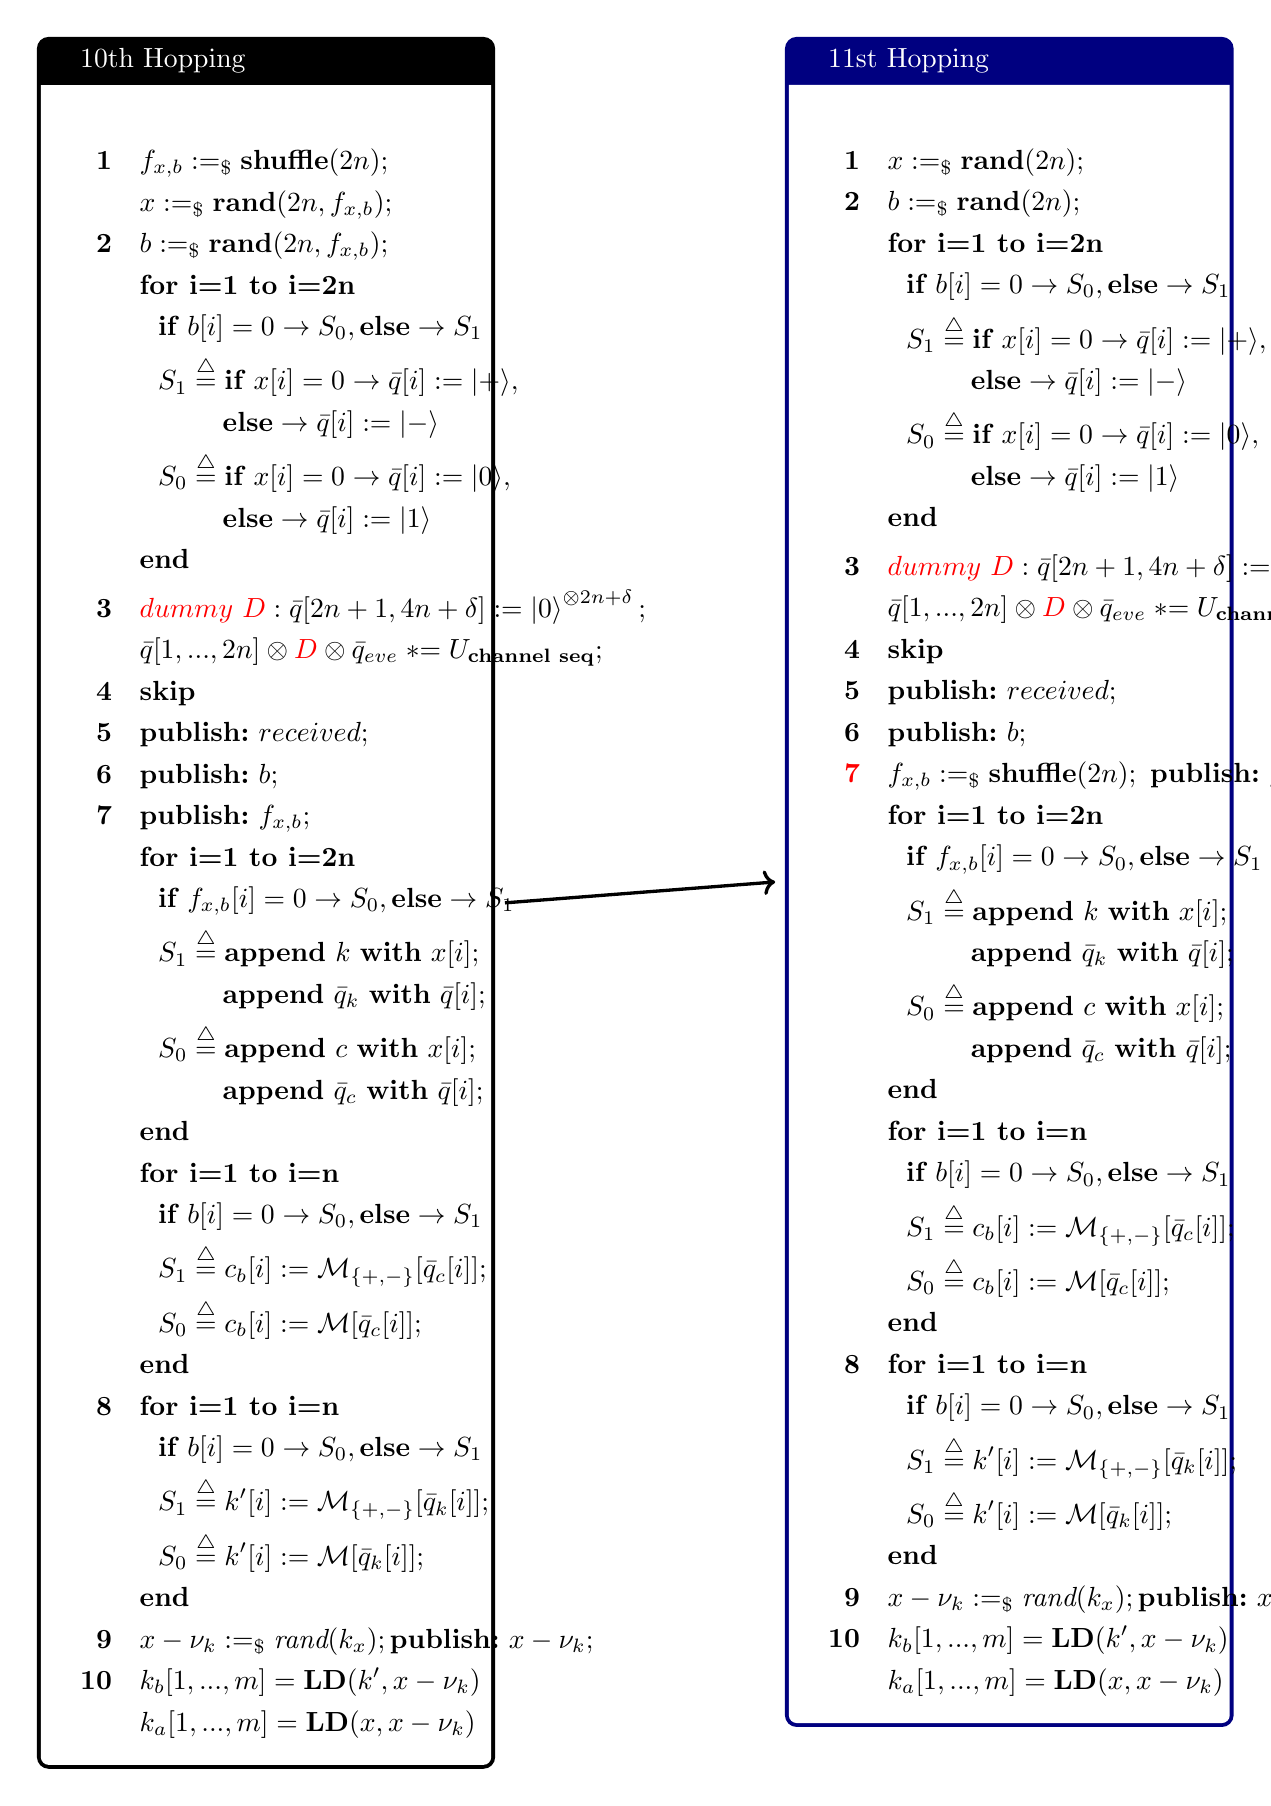
\begin{tikzpicture}[remember picture]

% Left box
\node[anchor=north west] (leftbox) at (0,0) {
\begin{minipage}[t]{0.48\textwidth}
\begin{tcolorbox}[colframe=black!50!black, colback=white, title=10th Hopping, width=\textwidth]
\begin{align*}
    \textbf{{1}} \quad 
    & f_{x,b}:=_\$\textbf{shuffle}(2n); \\
    &x :=_\$ \textbf{rand}(2n,f_{x,b}); \\ 
    \textbf{{2}}\quad 
    & b :=_\$ \textbf{rand}(2n,f_{x,b}); \\
    &\textbf{for i=1 to i=2n}\\
    &~~ \textbf{if }  b[i] = 0 \rightarrow S_{0} ,\textbf{else}\rightarrow S_{1}\\
    &~~ S_{1}\stackrel{\triangle}{=}\textbf{if }  x[i] = 0 \rightarrow \bar{q}[i] := |+\rangle,\\ &~~~~~~~~~\textbf{else}   \rightarrow \bar{q}[i] := |-\rangle\\
    &~~ S_{0}\stackrel{\triangle}{=}\textbf{if }  x[i] = 0 \rightarrow \bar{q}[i] := |0\rangle,\\ &~~~~~~~~~\textbf{else}   \rightarrow \bar{q}[i] := |1\rangle\\
    &\textbf{end}\\
    \textbf{{3}} 
    \quad & \textcolor{red}{dummy~D}: \bar{q}[2n+1,4n+\delta]:=\ket{0}^{\otimes 2n+\delta};\\     &\bar{q}[1,...,2n]\otimes \textcolor{red}{D} \otimes \bar{q}_{eve} \asteq U_{\textbf{channel seq}}; \\
    \textbf{{4}} \quad &\textbf{skip} \\ 
    \textbf{{5}} \quad & \textbf{publish:}~ received;\\
    \textbf{{6}} \quad & \textbf{publish:}~b;\\
    \textbf{{7}} 
    \quad & \textbf{publish:}~ f_{x,b};\\
    &\textbf{for i=1  to i=2n}\\
    &~~ \textbf{if }  f_{x,b}[i] = 0 \rightarrow S_{0} ,\textbf{else}\rightarrow S_{1}\\
    &~~ S_{1}\stackrel{\triangle}{=}\textbf{append}~k~\textbf{with}~x[i];\\
    &~~~~~~~~~\textbf{append}~\bar{q}_k~\textbf{with}~\bar{q}[i];\\
    &~~ S_{0}\stackrel{\triangle}{=}\textbf{append}~c~\textbf{with}~x[i];\\
    &~~~~~~~~~\textbf{append}~\bar{q}_c~\textbf{with}~\bar{q}[i];\\
    &\textbf{end}\\
    &\textbf{for i=1 to i=n}\\
    &~~ \textbf{if }  b[i] = 0 \rightarrow S_{0} ,\textbf{else}\rightarrow S_{1}\\
    &~~ S_{1}\stackrel{\triangle}{=}c_b[i]:= \mathcal{M}_{\{+,-\}} [\bar{q}_c[i]];\\
    &~~ S_{0}\stackrel{\triangle}{=}c_b[i]:= \mathcal{M} [\bar{q}_c[i]];\\
    &\textbf{end}\\
    \textbf{{8}}\quad 
    &\textbf{for i=1 to i=n}\\
    &~~ \textbf{if }  b[i] = 0 \rightarrow S_{0} ,\textbf{else}\rightarrow S_{1}\\
    &~~ S_{1}\stackrel{\triangle}{=}k'[i]:= \mathcal{M}_{\{+,-\}} [\bar{q}_k[i]];\\
    &~~ S_{0}\stackrel{\triangle}{=}k'[i]:= \mathcal{M} [\bar{q}_k[i]];\\
    &\textbf{end}\\
    \textbf{{9}} \quad & x-\nu_k :=_\$ \textit{rand}(k_x); \textbf{publish:}~ x-\nu_k;\\
    \textbf{{10}} \quad 
    &k_b[1,...,m]=\textbf{LD}(k',x-\nu_k)\\
    &k_a[1,...,m]=\textbf{LD}(x,x-\nu_k)
\end{align*}
\end{tcolorbox}
\end{minipage}
};

% Right box
\node[anchor=north west] (rightbox) at (9.5,0) {
\begin{minipage}[t]{0.47\textwidth}
\begin{tcolorbox}[colframe=blue!50!black, colback=white, title=11st Hopping, width=\textwidth]
\begin{align*}
    \textbf{{1}} \quad 
    &x :=_\$ \textbf{rand}(2n); \\ 
    \textbf{{2}}\quad 
    & b :=_\$ \textbf{rand}(2n); \\
    &\textbf{for i=1 to i=2n}\\
    &~~ \textbf{if }  b[i] = 0 \rightarrow S_{0} ,\textbf{else}\rightarrow S_{1}\\
    &~~ S_{1}\stackrel{\triangle}{=}\textbf{if }  x[i] = 0 \rightarrow \bar{q}[i] := |+\rangle,\\ &~~~~~~~~~\textbf{else}   \rightarrow \bar{q}[i] := |-\rangle\\
    &~~ S_{0}\stackrel{\triangle}{=}\textbf{if }  x[i] = 0 \rightarrow \bar{q}[i] := |0\rangle,\\ &~~~~~~~~~\textbf{else}   \rightarrow \bar{q}[i] := |1\rangle\\
    &\textbf{end}\\
    \textbf{{3}} 
    \quad & \textcolor{red}{dummy~D}: \bar{q}[2n+1,4n+\delta]:=\ket{0}^{\otimes 2n+\delta};\\     &\bar{q}[1,...,2n]\otimes \textcolor{red}{D} \otimes \bar{q}_{eve} \asteq U_{\textbf{channel seq}}; \\
    \textbf{{4}} \quad &\textbf{skip} \\ 
    \textbf{{5}} \quad & \textbf{publish:}~ received;\\
    \textbf{{6}} \quad & \textbf{publish:}~b;\\
    \textbf{\textcolor{red}{7}} 
    \quad &f_{x,b}:=_\$\textbf{shuffle}(2n); ~ \textbf{publish:}~ f_{x,b};\\
    &\textbf{for i=1  to i=2n}\\
    &~~ \textbf{if }  f_{x,b}[i] = 0 \rightarrow S_{0} ,\textbf{else}\rightarrow S_{1}\\
    &~~ S_{1}\stackrel{\triangle}{=}\textbf{append}~k~\textbf{with}~x[i];\\
    &~~~~~~~~~\textbf{append}~\bar{q}_k~\textbf{with}~\bar{q}[i];\\
    &~~ S_{0}\stackrel{\triangle}{=}\textbf{append}~c~\textbf{with}~x[i];\\
    &~~~~~~~~~\textbf{append}~\bar{q}_c~\textbf{with}~\bar{q}[i];\\
    &\textbf{end}\\
    &\textbf{for i=1 to i=n}\\
    &~~ \textbf{if }  b[i] = 0 \rightarrow S_{0} ,\textbf{else}\rightarrow S_{1}\\
    &~~ S_{1}\stackrel{\triangle}{=}c_b[i]:= \mathcal{M}_{\{+,-\}} [\bar{q}_c[i]];\\
    &~~ S_{0}\stackrel{\triangle}{=}c_b[i]:= \mathcal{M} [\bar{q}_c[i]];\\
    &\textbf{end}\\
    \textbf{{8}}\quad 
    &\textbf{for i=1 to i=n}\\
    &~~ \textbf{if }  b[i] = 0 \rightarrow S_{0} ,\textbf{else}\rightarrow S_{1}\\
    &~~ S_{1}\stackrel{\triangle}{=}k'[i]:= \mathcal{M}_{\{+,-\}} [\bar{q}_k[i]];\\
    &~~ S_{0}\stackrel{\triangle}{=}k'[i]:= \mathcal{M} [\bar{q}_k[i]];\\
    &\textbf{end}\\
    \textbf{{9}} \quad & x-\nu_k :=_\$ \textit{rand}(k_x); \textbf{publish:}~ x-\nu_k;\\
    \textbf{{10}} \quad 
    &k_b[1,...,m]=\textbf{LD}(k',x-\nu_k)\\
    &k_a[1,...,m]=\textbf{LD}(x,x-\nu_k)
\end{align*}
\end{tcolorbox}
\end{minipage}
};

% Draw arrow between boxes
\draw[->, very thick] (leftbox.east) -- node[above]{} (rightbox.west);

\end{tikzpicture}
\newpage


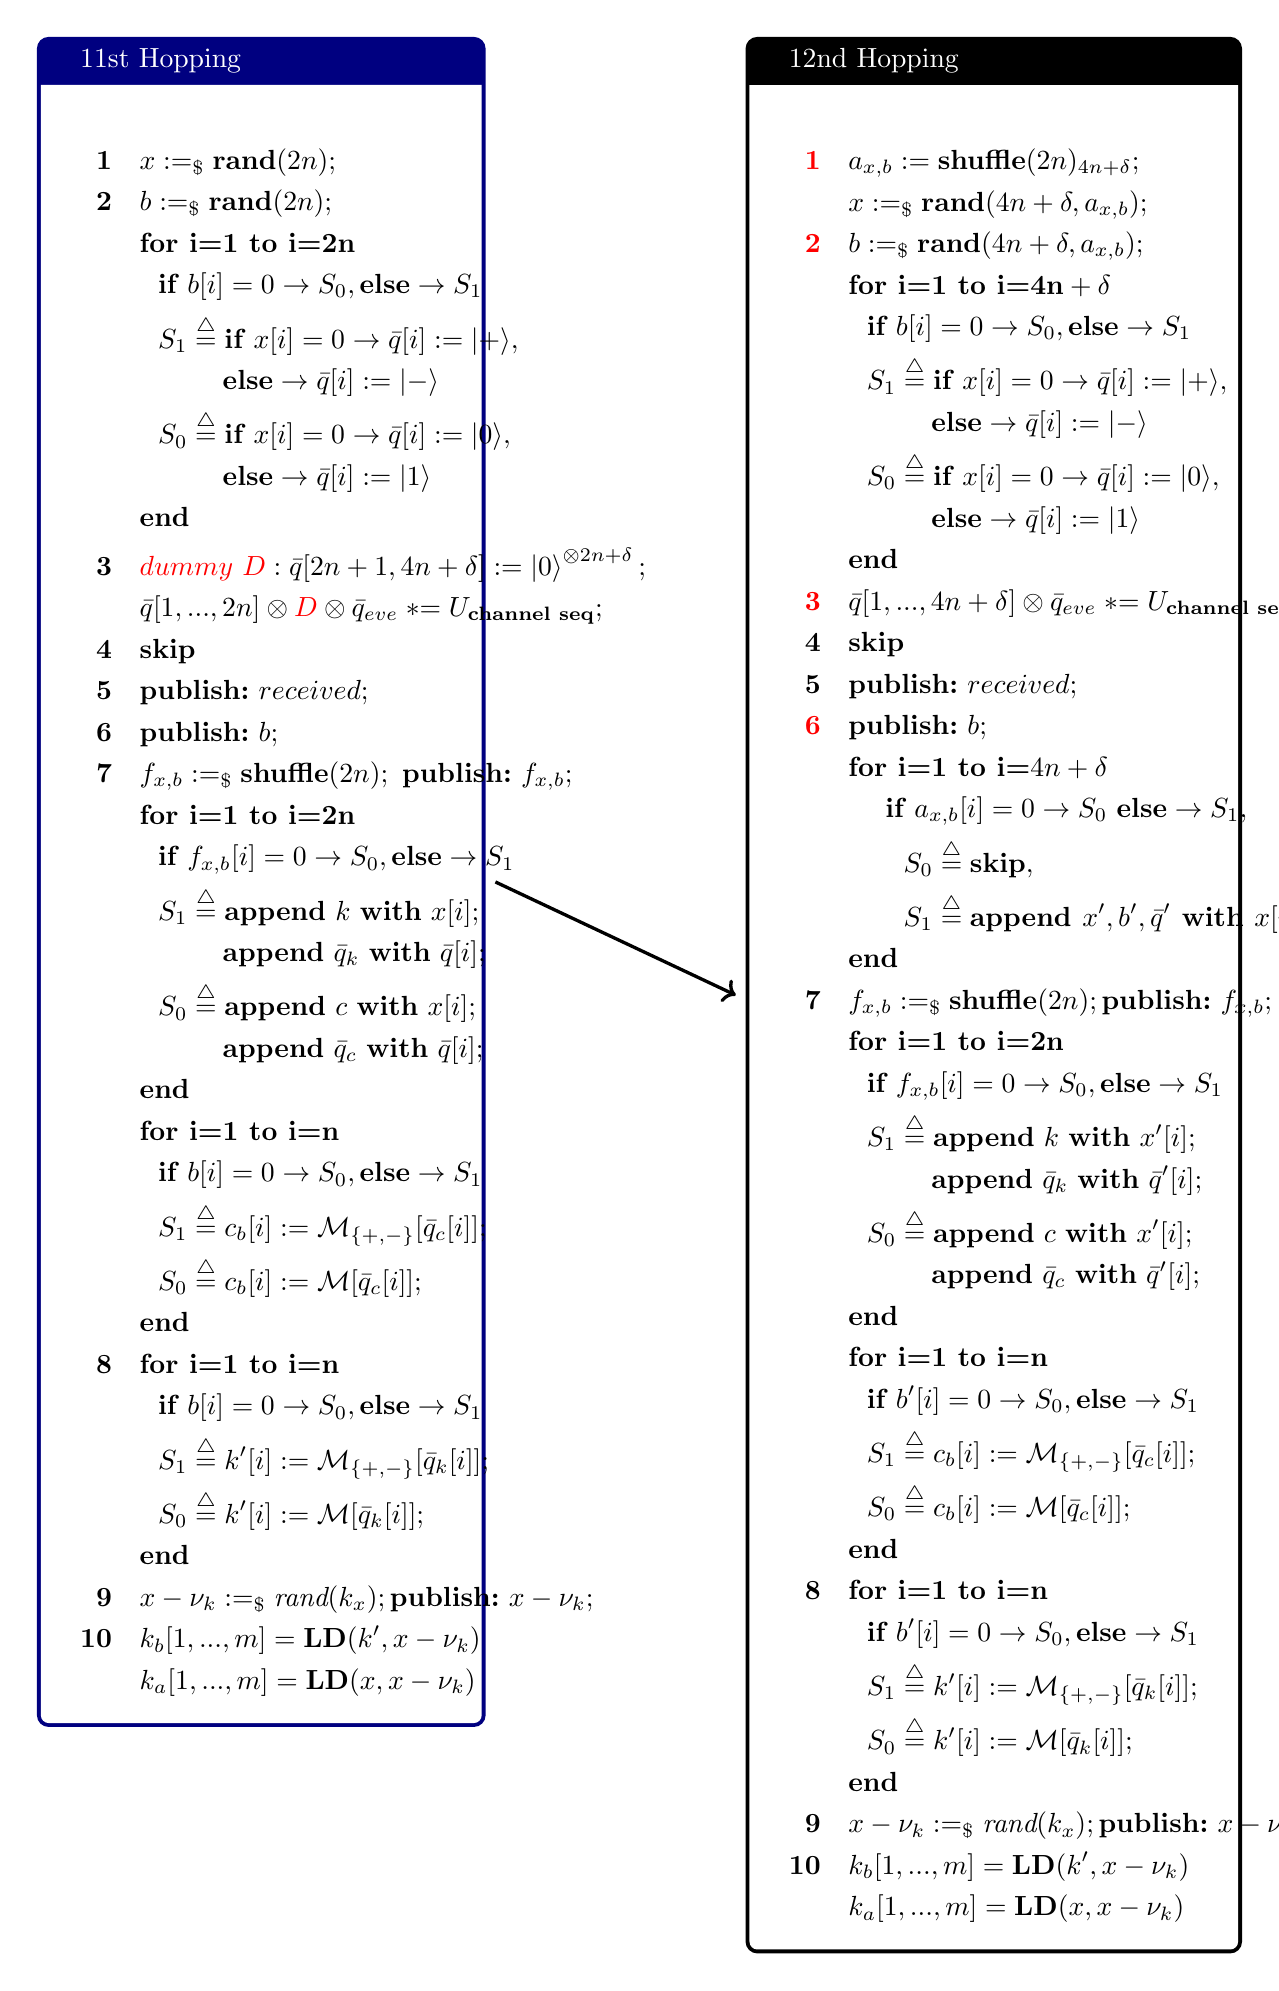
\begin{tikzpicture}[remember picture]

% Left box
\node[anchor=north west] (leftbox) at (0,0) {
\begin{minipage}[t]{0.47\textwidth}
\begin{tcolorbox}[colframe=blue!50!black, colback=white, title=11st Hopping, width=\textwidth]
\begin{align*}
    \textbf{{1}} \quad 
    &x :=_\$ \textbf{rand}(2n); \\ 
    \textbf{{2}}\quad 
    & b :=_\$ \textbf{rand}(2n); \\
    &\textbf{for i=1 to i=2n}\\
    &~~ \textbf{if }  b[i] = 0 \rightarrow S_{0} ,\textbf{else}\rightarrow S_{1}\\
    &~~ S_{1}\stackrel{\triangle}{=}\textbf{if }  x[i] = 0 \rightarrow \bar{q}[i] := |+\rangle,\\ &~~~~~~~~~\textbf{else}   \rightarrow \bar{q}[i] := |-\rangle\\
    &~~ S_{0}\stackrel{\triangle}{=}\textbf{if }  x[i] = 0 \rightarrow \bar{q}[i] := |0\rangle,\\ &~~~~~~~~~\textbf{else}   \rightarrow \bar{q}[i] := |1\rangle\\
    &\textbf{end}\\
    \textbf{{3}} 
    \quad & \textcolor{red}{dummy~D}: \bar{q}[2n+1,4n+\delta]:=\ket{0}^{\otimes 2n+\delta};\\     &\bar{q}[1,...,2n]\otimes \textcolor{red}{D} \otimes \bar{q}_{eve} \asteq U_{\textbf{channel seq}}; \\
    \textbf{{4}} \quad &\textbf{skip} \\ 
    \textbf{{5}} \quad & \textbf{publish:}~ received;\\
    \textbf{{6}} \quad & \textbf{publish:}~b;\\
    \textbf{{7}} 
    \quad &f_{x,b}:=_\$\textbf{shuffle}(2n); ~ \textbf{publish:}~ f_{x,b};\\
    &\textbf{for i=1  to i=2n}\\
    &~~ \textbf{if }  f_{x,b}[i] = 0 \rightarrow S_{0} ,\textbf{else}\rightarrow S_{1}\\
    &~~ S_{1}\stackrel{\triangle}{=}\textbf{append}~k~\textbf{with}~x[i];\\
    &~~~~~~~~~\textbf{append}~\bar{q}_k~\textbf{with}~\bar{q}[i];\\
    &~~ S_{0}\stackrel{\triangle}{=}\textbf{append}~c~\textbf{with}~x[i];\\
    &~~~~~~~~~\textbf{append}~\bar{q}_c~\textbf{with}~\bar{q}[i];\\
    &\textbf{end}\\
    &\textbf{for i=1 to i=n}\\
    &~~ \textbf{if }  b[i] = 0 \rightarrow S_{0} ,\textbf{else}\rightarrow S_{1}\\
    &~~ S_{1}\stackrel{\triangle}{=}c_b[i]:= \mathcal{M}_{\{+,-\}} [\bar{q}_c[i]];\\
    &~~ S_{0}\stackrel{\triangle}{=}c_b[i]:= \mathcal{M} [\bar{q}_c[i]];\\
    &\textbf{end}\\
    \textbf{{8}}\quad 
    &\textbf{for i=1 to i=n}\\
    &~~ \textbf{if }  b[i] = 0 \rightarrow S_{0} ,\textbf{else}\rightarrow S_{1}\\
    &~~ S_{1}\stackrel{\triangle}{=}k'[i]:= \mathcal{M}_{\{+,-\}} [\bar{q}_k[i]];\\
    &~~ S_{0}\stackrel{\triangle}{=}k'[i]:= \mathcal{M} [\bar{q}_k[i]];\\
    &\textbf{end}\\
    \textbf{{9}} \quad & x-\nu_k :=_\$ \textit{rand}(k_x); \textbf{publish:}~ x-\nu_k;\\
    \textbf{{10}} \quad 
    &k_b[1,...,m]=\textbf{LD}(k',x-\nu_k)\\
    &k_a[1,...,m]=\textbf{LD}(x,x-\nu_k)
\end{align*}
\end{tcolorbox}
\end{minipage}
};

% Right box
\node[anchor=north west] (rightbox) at (9,0) {
\begin{minipage}[t]{0.52\textwidth}
\begin{tcolorbox}[colframe=black!50!black, colback=white, title=12nd Hopping, width=\textwidth]
\begin{align*}
    \textbf{\textcolor{red}{1}} \quad 
    & a_{x,b}:=\textbf{shuffle}(2n)_{4n+\delta};\\
    &x :=_\$ \textbf{rand}(4n+\delta,a_{x,b}); \\ 
    \textbf{\textcolor{red}{2}}\quad 
    & b :=_\$ \textbf{rand}(4n+\delta,a_{x,b}); \\
    &\textbf{for i=1 to i=4n}+\delta\\
    &~~ \textbf{if }  b[i] = 0 \rightarrow S_{0} ,\textbf{else}\rightarrow S_{1}\\
    &~~ S_{1}\stackrel{\triangle}{=}\textbf{if }  x[i] = 0 \rightarrow \bar{q}[i] := |+\rangle,\\ &~~~~~~~~~\textbf{else}   \rightarrow \bar{q}[i] := |-\rangle\\
    &~~ S_{0}\stackrel{\triangle}{=}\textbf{if }  x[i] = 0 \rightarrow \bar{q}[i] := |0\rangle,\\ &~~~~~~~~~\textbf{else}   \rightarrow \bar{q}[i] := |1\rangle\\
    &\textbf{end}\\
    \textbf{\textcolor{red}{3}} 
    \quad & \bar{q}[1,...,4n+\delta] \otimes \bar{q}_{eve} \asteq U_{\textbf{channel seq}}; \\
    \textbf{{4}} \quad &\textbf{skip} \\ 
    \textbf{{5}} \quad & \textbf{publish:}~ received;\\
    \textbf{\textcolor{red}{6}} \quad & \textbf{publish:}~b;\\
    &\textbf{for i=1 to i=} 4n+\delta\\
    &~~~~ \textbf{if }  a_{x,b}[i] = 0 \rightarrow S_{0} ~\textbf{else} \rightarrow S_{1} ,\\
    &~~~~~~S_{0}\stackrel{\triangle}{=}\textbf{skip},\\
    &~~~~~~S_{1}\stackrel{\triangle}{=}\textbf{append } x',b',\bar{q}' \textbf{ with } x[i],b[i],\bar{q}[i]\\
    &\textbf{end}\\
    \textbf{{7}} 
    \quad & f_{x,b}:=_\$\textbf{shuffle}(2n); \textbf{publish:}~ f_{x,b};\\
    &\textbf{for i=1  to i=2n}\\
    &~~ \textbf{if }  f_{x,b}[i] = 0 \rightarrow S_{0} ,\textbf{else}\rightarrow S_{1}\\
    &~~ S_{1}\stackrel{\triangle}{=}\textbf{append}~k~\textbf{with}~x'[i];\\
    &~~~~~~~~~\textbf{append}~\bar{q}_k~\textbf{with}~\bar{q}'[i];\\
    &~~ S_{0}\stackrel{\triangle}{=}\textbf{append}~c~\textbf{with}~x'[i];\\
    &~~~~~~~~~\textbf{append}~\bar{q}_c~\textbf{with}~\bar{q}'[i];\\
    &\textbf{end}\\
    &\textbf{for i=1 to i=n}\\
    &~~ \textbf{if }  b'[i] = 0 \rightarrow S_{0} ,\textbf{else}\rightarrow S_{1}\\
    &~~ S_{1}\stackrel{\triangle}{=}c_b[i]:= \mathcal{M}_{\{+,-\}} [\bar{q}_c[i]];\\
    &~~ S_{0}\stackrel{\triangle}{=}c_b[i]:= \mathcal{M} [\bar{q}_c[i]];\\
    &\textbf{end}\\
    \textbf{{8}}\quad 
    &\textbf{for i=1 to i=n}\\
    &~~ \textbf{if }  b'[i] = 0 \rightarrow S_{0} ,\textbf{else}\rightarrow S_{1}\\
    &~~ S_{1}\stackrel{\triangle}{=}k'[i]:= \mathcal{M}_{\{+,-\}} [\bar{q}_k[i]];\\
    &~~ S_{0}\stackrel{\triangle}{=}k'[i]:= \mathcal{M} [\bar{q}_k[i]];\\
    &\textbf{end}\\
    \textbf{{9}} \quad & x-\nu_k :=_\$ \textit{rand}(k_x); \textbf{publish:}~ x-\nu_k;\\
    \textbf{{10}} \quad 
    &k_b[1,...,m]=\textbf{LD}(k',x-\nu_k)\\
    &k_a[1,...,m]=\textbf{LD}(x,x-\nu_k)
\end{align*}
\end{tcolorbox}
\end{minipage}
};

% Draw arrow between boxes
\draw[->, very thick] (leftbox.east) -- node[above]{} (rightbox.west);

\end{tikzpicture}
\newpage

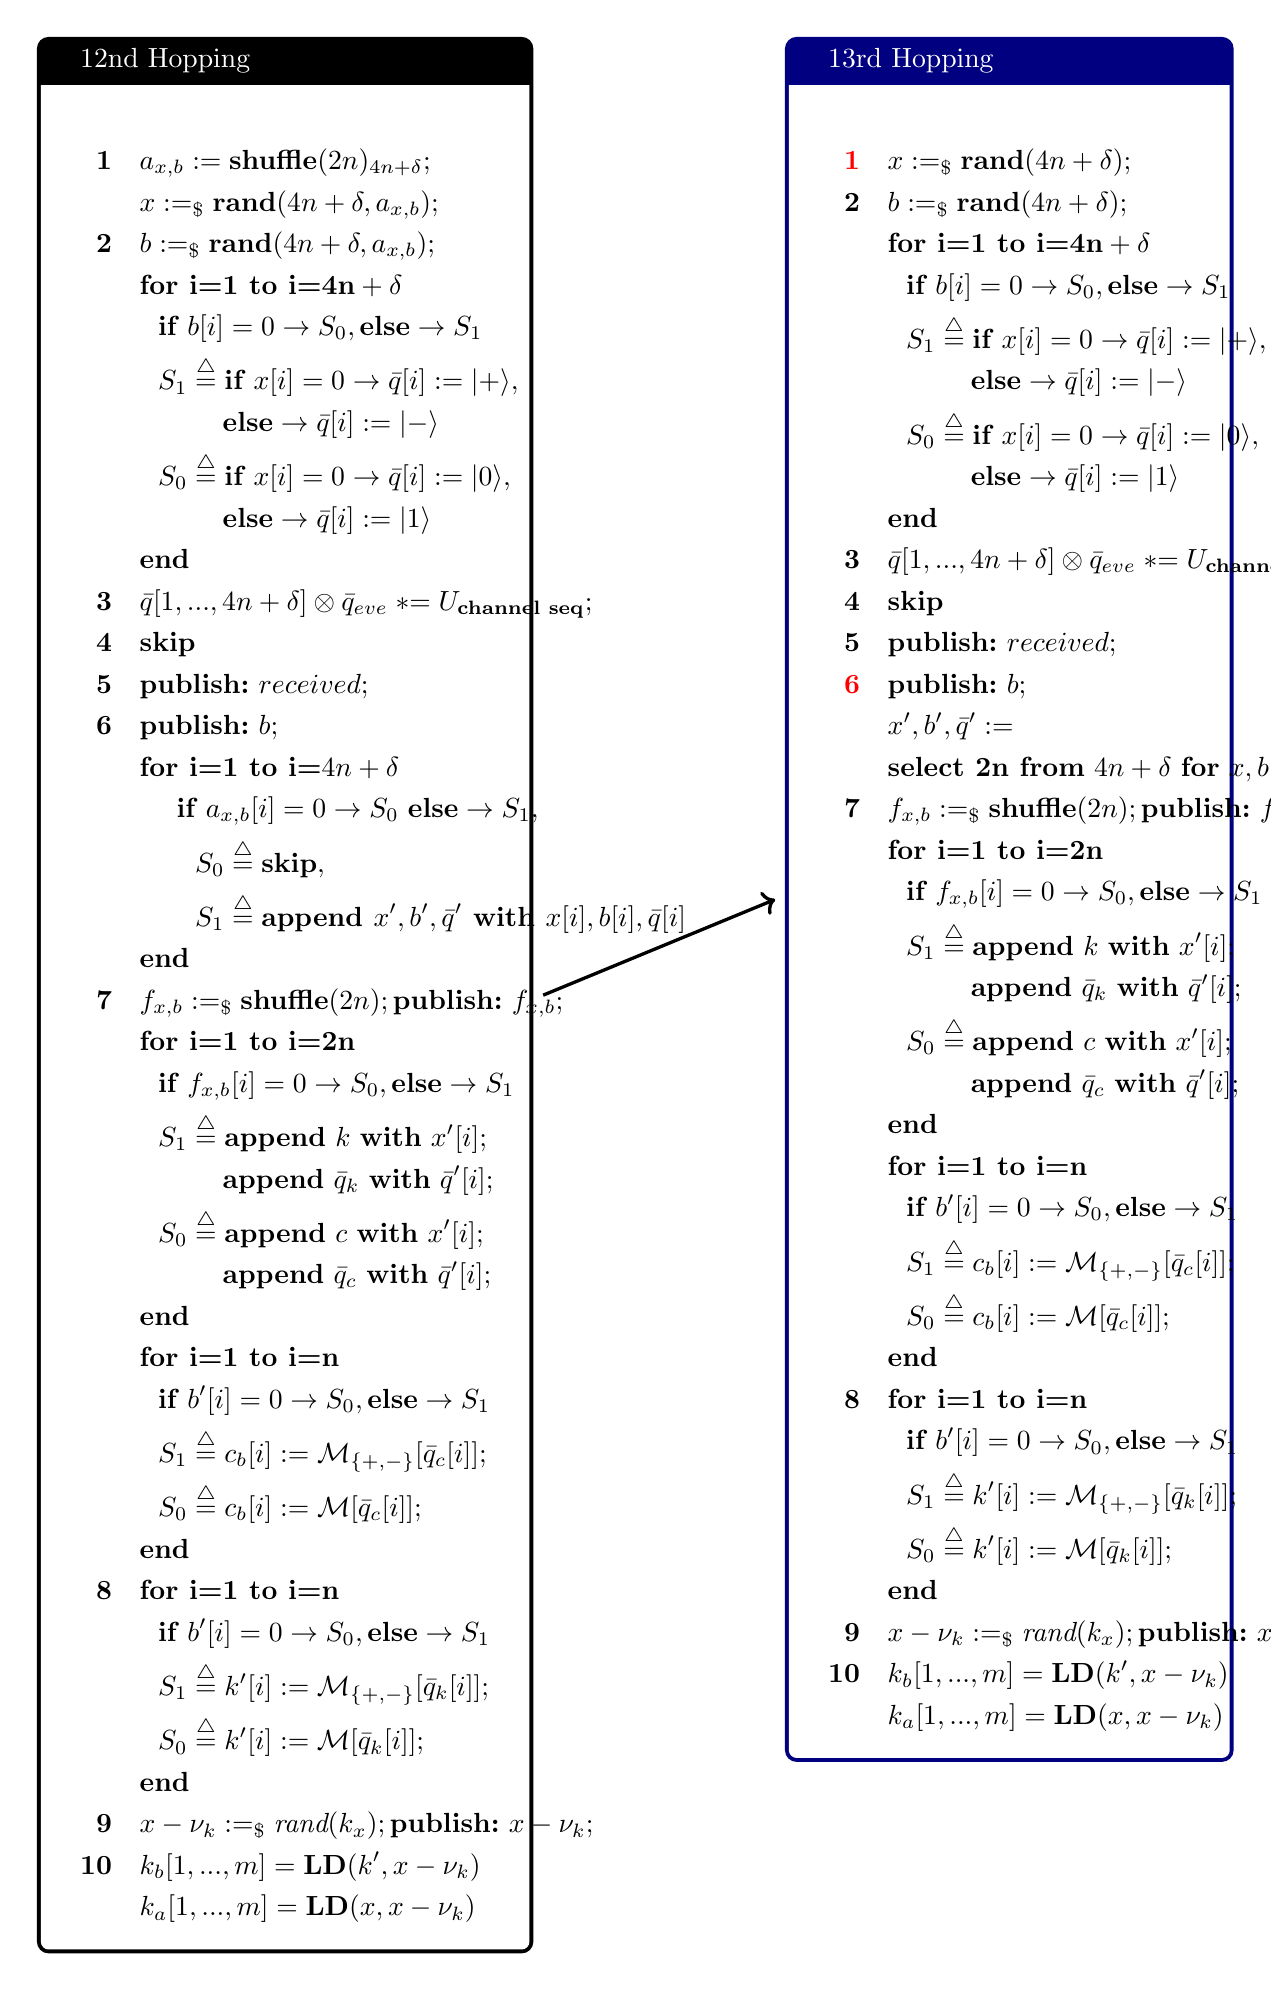
\begin{tikzpicture}[remember picture]

% Left box
\node[anchor=north west] (leftbox) at (0,0) {
\begin{minipage}[t]{0.52\textwidth}
\begin{tcolorbox}[colframe=black!50!black, colback=white, title=12nd Hopping, width=\textwidth]
\begin{align*}
    \textbf{{1}} \quad 
    & a_{x,b}:=\textbf{shuffle}(2n)_{4n+\delta};\\
    &x :=_\$ \textbf{rand}(4n+\delta,a_{x,b}); \\ 
    \textbf{{2}}\quad 
    & b :=_\$ \textbf{rand}(4n+\delta,a_{x,b}); \\
    &\textbf{for i=1 to i=4n}+\delta\\
    &~~ \textbf{if }  b[i] = 0 \rightarrow S_{0} ,\textbf{else}\rightarrow S_{1}\\
    &~~ S_{1}\stackrel{\triangle}{=}\textbf{if }  x[i] = 0 \rightarrow \bar{q}[i] := |+\rangle,\\ &~~~~~~~~~\textbf{else}   \rightarrow \bar{q}[i] := |-\rangle\\
    &~~ S_{0}\stackrel{\triangle}{=}\textbf{if }  x[i] = 0 \rightarrow \bar{q}[i] := |0\rangle,\\ &~~~~~~~~~\textbf{else}   \rightarrow \bar{q}[i] := |1\rangle\\
    &\textbf{end}\\
    \textbf{{3}} 
    \quad & \bar{q}[1,...,4n+\delta] \otimes \bar{q}_{eve} \asteq U_{\textbf{channel seq}}; \\
    \textbf{{4}} \quad &\textbf{skip} \\ 
    \textbf{{5}} \quad & \textbf{publish:}~ received;\\
    \textbf{{6}} \quad & \textbf{publish:}~b;\\
    &\textbf{for i=1 to i=} 4n+\delta\\
    &~~~~ \textbf{if }  a_{x,b}[i] = 0 \rightarrow S_{0} ~\textbf{else} \rightarrow S_{1} ,\\
    &~~~~~~S_{0}\stackrel{\triangle}{=}\textbf{skip},\\
    &~~~~~~S_{1}\stackrel{\triangle}{=}\textbf{append } x',b',\bar{q}' \textbf{ with } x[i],b[i],\bar{q}[i]\\
    &\textbf{end}\\
    \textbf{{7}} 
    \quad & f_{x,b}:=_\$\textbf{shuffle}(2n); \textbf{publish:}~ f_{x,b};\\
    &\textbf{for i=1  to i=2n}\\
    &~~ \textbf{if }  f_{x,b}[i] = 0 \rightarrow S_{0} ,\textbf{else}\rightarrow S_{1}\\
    &~~ S_{1}\stackrel{\triangle}{=}\textbf{append}~k~\textbf{with}~x'[i];\\
    &~~~~~~~~~\textbf{append}~\bar{q}_k~\textbf{with}~\bar{q}'[i];\\
    &~~ S_{0}\stackrel{\triangle}{=}\textbf{append}~c~\textbf{with}~x'[i];\\
    &~~~~~~~~~\textbf{append}~\bar{q}_c~\textbf{with}~\bar{q}'[i];\\
    &\textbf{end}\\
    &\textbf{for i=1 to i=n}\\
    &~~ \textbf{if }  b'[i] = 0 \rightarrow S_{0} ,\textbf{else}\rightarrow S_{1}\\
    &~~ S_{1}\stackrel{\triangle}{=}c_b[i]:= \mathcal{M}_{\{+,-\}} [\bar{q}_c[i]];\\
    &~~ S_{0}\stackrel{\triangle}{=}c_b[i]:= \mathcal{M} [\bar{q}_c[i]];\\
    &\textbf{end}\\
    \textbf{{8}}\quad 
    &\textbf{for i=1 to i=n}\\
    &~~ \textbf{if }  b'[i] = 0 \rightarrow S_{0} ,\textbf{else}\rightarrow S_{1}\\
    &~~ S_{1}\stackrel{\triangle}{=}k'[i]:= \mathcal{M}_{\{+,-\}} [\bar{q}_k[i]];\\
    &~~ S_{0}\stackrel{\triangle}{=}k'[i]:= \mathcal{M} [\bar{q}_k[i]];\\
    &\textbf{end}\\
    \textbf{{9}} \quad & x-\nu_k :=_\$ \textit{rand}(k_x); \textbf{publish:}~ x-\nu_k;\\
    \textbf{{10}} \quad 
    &k_b[1,...,m]=\textbf{LD}(k',x-\nu_k)\\
    &k_a[1,...,m]=\textbf{LD}(x,x-\nu_k)
\end{align*}
\end{tcolorbox}
\end{minipage}
};

% Right box
\node[anchor=north west] (rightbox) at (9.5,0) {
\begin{minipage}[t]{0.47\textwidth}
\begin{tcolorbox}[colframe=blue!50!black, colback=white, title=13rd Hopping, width=\textwidth]
\begin{align*}
    \textbf{\textcolor{red}{1}} \quad 
    & x :=_\$ \textbf{rand}(4n+\delta); \\ 
    \textbf{{2}}\quad 
    & b :=_\$ \textbf{rand}(4n+\delta); \\
    &\textbf{for i=1 to i=4n}+\delta\\
    &~~ \textbf{if }  b[i] = 0 \rightarrow S_{0} ,\textbf{else}\rightarrow S_{1}\\
    &~~ S_{1}\stackrel{\triangle}{=}\textbf{if }  x[i] = 0 \rightarrow \bar{q}[i] := |+\rangle,\\ &~~~~~~~~~\textbf{else}   \rightarrow \bar{q}[i] := |-\rangle\\
    &~~ S_{0}\stackrel{\triangle}{=}\textbf{if }  x[i] = 0 \rightarrow \bar{q}[i] := |0\rangle,\\ &~~~~~~~~~\textbf{else}   \rightarrow \bar{q}[i] := |1\rangle\\
    &\textbf{end}\\
    \textbf{{3}} 
    \quad & \bar{q}[1,...,4n+\delta] \otimes \bar{q}_{eve} \asteq U_{\textbf{channel seq}}; \\
    \textbf{{4}} \quad &\textbf{skip} \\ 
    \textbf{{5}} \quad & \textbf{publish:}~ received;\\
    \textbf{\textcolor{red}{6}} \quad & \textbf{publish:}~b;\\
     &x',b',\bar{q}':=\\&\textbf{select 2n from}~4n+\delta ~\textbf{for}~ x,b,\bar{q};\\ 
    \textbf{{7}} 
    \quad & f_{x,b}:=_\$\textbf{shuffle}(2n); \textbf{publish:}~ f_{x,b};\\
    &\textbf{for i=1  to i=2n}\\
    &~~ \textbf{if }  f_{x,b}[i] = 0 \rightarrow S_{0} ,\textbf{else}\rightarrow S_{1}\\
    &~~ S_{1}\stackrel{\triangle}{=}\textbf{append}~k~\textbf{with}~x'[i];\\
    &~~~~~~~~~\textbf{append}~\bar{q}_k~\textbf{with}~\bar{q}'[i];\\
    &~~ S_{0}\stackrel{\triangle}{=}\textbf{append}~c~\textbf{with}~x'[i];\\
    &~~~~~~~~~\textbf{append}~\bar{q}_c~\textbf{with}~\bar{q}'[i];\\
    &\textbf{end}\\
    &\textbf{for i=1 to i=n}\\
    &~~ \textbf{if }  b'[i] = 0 \rightarrow S_{0} ,\textbf{else}\rightarrow S_{1}\\
    &~~ S_{1}\stackrel{\triangle}{=}c_b[i]:= \mathcal{M}_{\{+,-\}} [\bar{q}_c[i]];\\
    &~~ S_{0}\stackrel{\triangle}{=}c_b[i]:= \mathcal{M} [\bar{q}_c[i]];\\
    &\textbf{end}\\
    \textbf{{8}}\quad 
    &\textbf{for i=1 to i=n}\\
    &~~ \textbf{if }  b'[i] = 0 \rightarrow S_{0} ,\textbf{else}\rightarrow S_{1}\\
    &~~ S_{1}\stackrel{\triangle}{=}k'[i]:= \mathcal{M}_{\{+,-\}} [\bar{q}_k[i]];\\
    &~~ S_{0}\stackrel{\triangle}{=}k'[i]:= \mathcal{M} [\bar{q}_k[i]];\\
    &\textbf{end}\\
    \textbf{{9}} \quad & x-\nu_k :=_\$ \textit{rand}(k_x); \textbf{publish:}~ x-\nu_k;\\
    \textbf{{10}} \quad 
    &k_b[1,...,m]=\textbf{LD}(k',x-\nu_k)\\
    &k_a[1,...,m]=\textbf{LD}(x,x-\nu_k)
\end{align*}
\end{tcolorbox}
\end{minipage}
};

% Draw arrow between boxes
\draw[->, very thick] (leftbox.east) -- node[above]{} (rightbox.west);

\end{tikzpicture}
\newpage

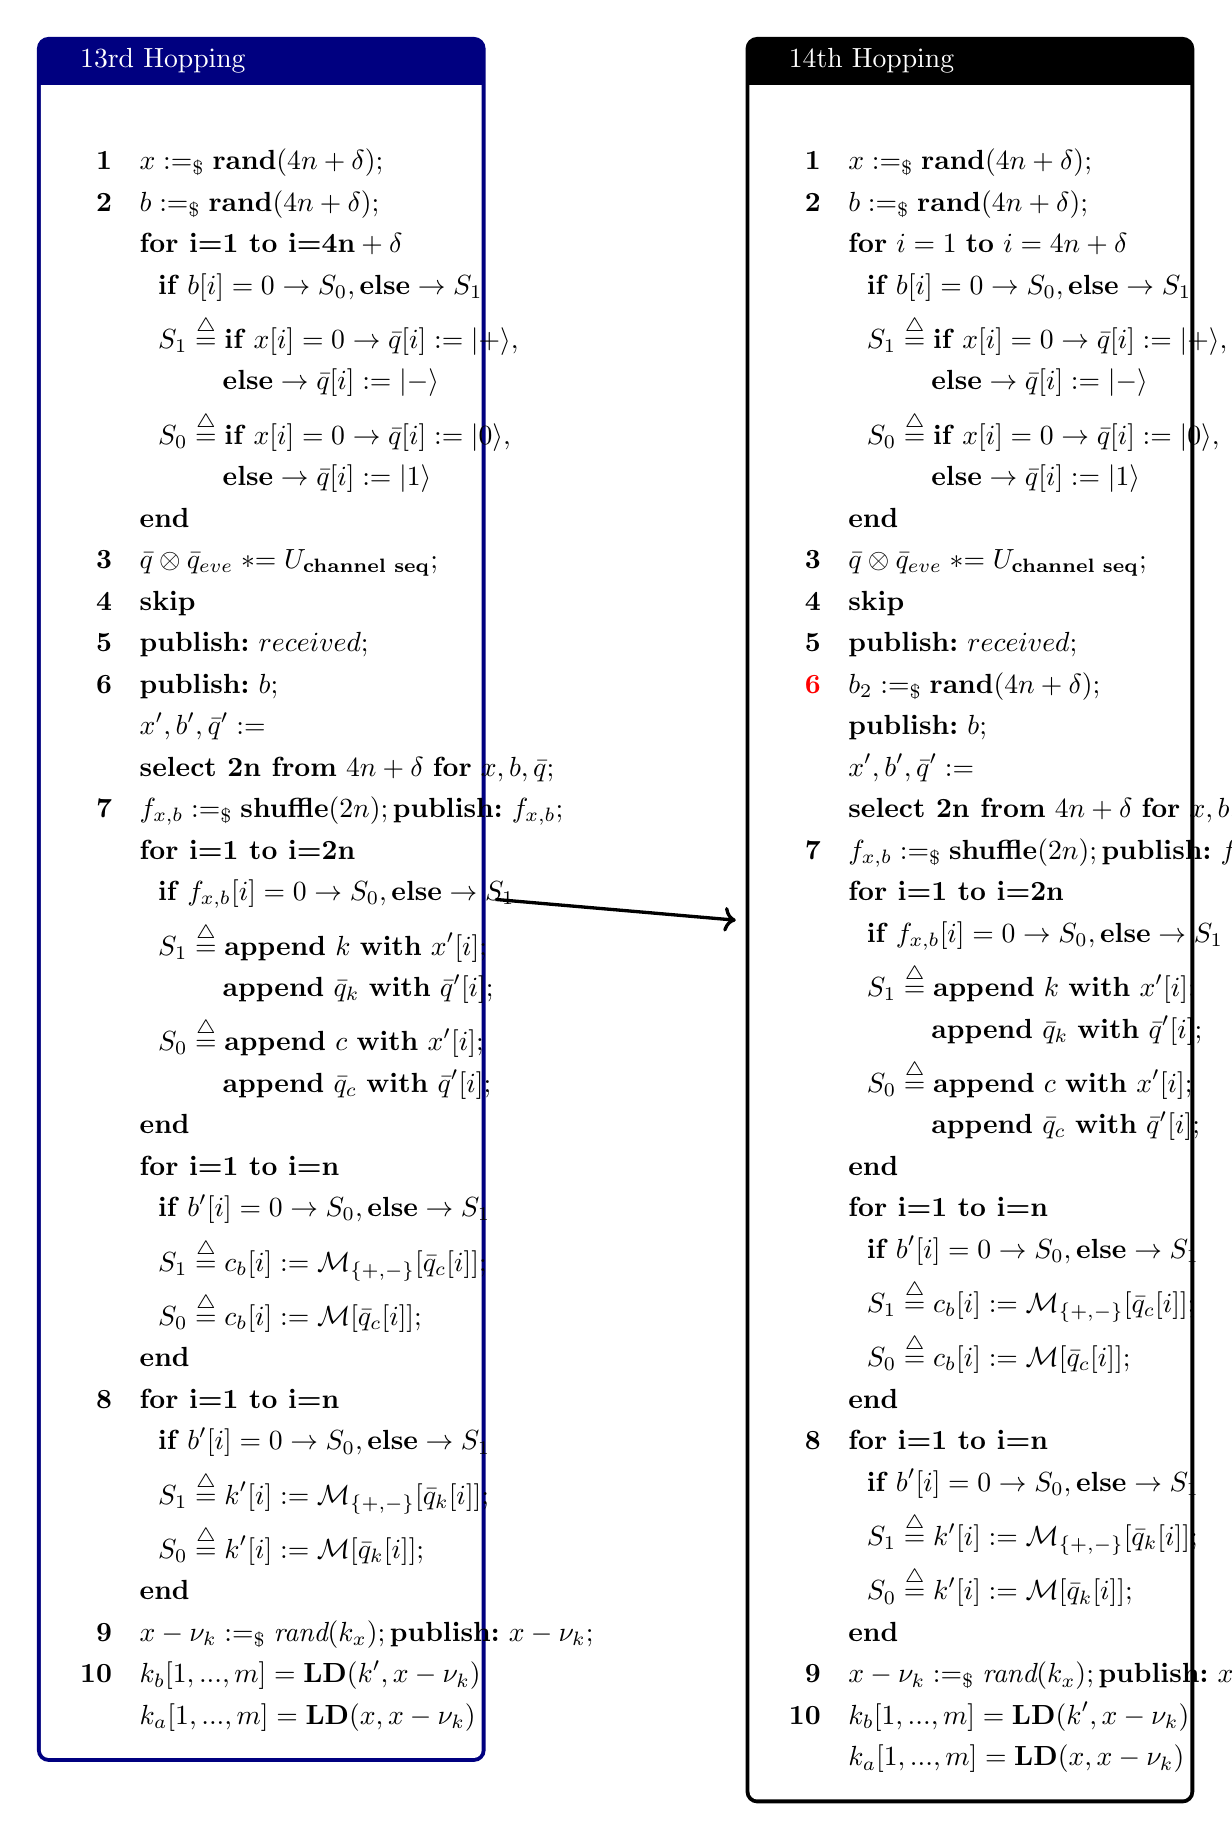
\begin{tikzpicture}[remember picture]

% Left box
\node[anchor=north west] (leftbox) at (0,0) {
\begin{minipage}[t]{0.47\textwidth}
\begin{tcolorbox}[colframe=blue!50!black, colback=white, title=13rd Hopping, width=\textwidth]
\begin{align*}
    \textbf{{1}} \quad 
    & x :=_\$ \textbf{rand}(4n+\delta); \\ 
    \textbf{{2}}\quad 
    & b :=_\$ \textbf{rand}(4n+\delta); \\
    &\textbf{for i=1 to i=4n}+\delta\\
    &~~ \textbf{if }  b[i] = 0 \rightarrow S_{0} ,\textbf{else}\rightarrow S_{1}\\
    &~~ S_{1}\stackrel{\triangle}{=}\textbf{if }  x[i] = 0 \rightarrow \bar{q}[i] := |+\rangle,\\ &~~~~~~~~~\textbf{else}   \rightarrow \bar{q}[i] := |-\rangle\\
    &~~ S_{0}\stackrel{\triangle}{=}\textbf{if }  x[i] = 0 \rightarrow \bar{q}[i] := |0\rangle,\\ &~~~~~~~~~\textbf{else}   \rightarrow \bar{q}[i] := |1\rangle\\
    &\textbf{end}\\
    \textbf{{3}} 
    \quad & \bar{q} \otimes \bar{q}_{eve} \asteq U_{\textbf{channel seq}}; \\
    \textbf{{4}} \quad &\textbf{skip} \\ 
    \textbf{{5}} \quad & \textbf{publish:}~ received;\\
    \textbf{{6}} \quad & \textbf{publish:}~b;\\
     &x',b',\bar{q}':=\\&\textbf{select 2n from}~4n+\delta ~\textbf{for}~ x,b,\bar{q};\\ 
    \textbf{{7}} 
    \quad & f_{x,b}:=_\$\textbf{shuffle}(2n); \textbf{publish:}~ f_{x,b};\\
    &\textbf{for i=1  to i=2n}\\
    &~~ \textbf{if }  f_{x,b}[i] = 0 \rightarrow S_{0} ,\textbf{else}\rightarrow S_{1}\\
    &~~ S_{1}\stackrel{\triangle}{=}\textbf{append}~k~\textbf{with}~x'[i];\\
    &~~~~~~~~~\textbf{append}~\bar{q}_k~\textbf{with}~\bar{q}'[i];\\
    &~~ S_{0}\stackrel{\triangle}{=}\textbf{append}~c~\textbf{with}~x'[i];\\
    &~~~~~~~~~\textbf{append}~\bar{q}_c~\textbf{with}~\bar{q}'[i];\\
    &\textbf{end}\\
    &\textbf{for i=1 to i=n}\\
    &~~ \textbf{if }  b'[i] = 0 \rightarrow S_{0} ,\textbf{else}\rightarrow S_{1}\\
    &~~ S_{1}\stackrel{\triangle}{=}c_b[i]:= \mathcal{M}_{\{+,-\}} [\bar{q}_c[i]];\\
    &~~ S_{0}\stackrel{\triangle}{=}c_b[i]:= \mathcal{M} [\bar{q}_c[i]];\\
    &\textbf{end}\\
    \textbf{{8}}\quad 
    &\textbf{for i=1 to i=n}\\
    &~~ \textbf{if }  b'[i] = 0 \rightarrow S_{0} ,\textbf{else}\rightarrow S_{1}\\
    &~~ S_{1}\stackrel{\triangle}{=}k'[i]:= \mathcal{M}_{\{+,-\}} [\bar{q}_k[i]];\\
    &~~ S_{0}\stackrel{\triangle}{=}k'[i]:= \mathcal{M} [\bar{q}_k[i]];\\
    &\textbf{end}\\
    \textbf{{9}} \quad & x-\nu_k :=_\$ \textit{rand}(k_x); \textbf{publish:}~ x-\nu_k;\\
    \textbf{{10}} \quad 
    &k_b[1,...,m]=\textbf{LD}(k',x-\nu_k)\\
    &k_a[1,...,m]=\textbf{LD}(x,x-\nu_k)
\end{align*}
\end{tcolorbox}
\end{minipage}
};

% Right box
\node[anchor=north west] (rightbox) at (9,0) {
\begin{minipage}[t]{0.47\textwidth}
\begin{tcolorbox}[colframe=black!50!black, colback=white, title=14th Hopping, width=\textwidth]
\begin{align*}
    \textbf{{1}} \quad 
    & x :=_\$ \textbf{rand}(4n+\delta); \\ 
    \textbf{{2}}\quad 
    & b :=_\$ \textbf{rand}(4n+\delta); \\
    &\textbf{for} ~i=1 ~\textbf{to}~ i=4n+\delta\\
    &~~ \textbf{if }  b[i] = 0 \rightarrow S_{0} ,\textbf{else}\rightarrow S_{1}\\
    &~~ S_{1}\stackrel{\triangle}{=}\textbf{if }  x[i] = 0 \rightarrow \bar{q}[i] := |+\rangle,\\ &~~~~~~~~~\textbf{else}   \rightarrow \bar{q}[i] := |-\rangle\\
    &~~ S_{0}\stackrel{\triangle}{=}\textbf{if }  x[i] = 0 \rightarrow \bar{q}[i] := |0\rangle,\\ &~~~~~~~~~\textbf{else}   \rightarrow \bar{q}[i] := |1\rangle\\
    &\textbf{end}\\
    \textbf{{3}} 
    \quad & \bar{q}\otimes \bar{q}_{eve} \asteq U_{\textbf{channel seq}}; \\
    \textbf{{4}} \quad &\textbf{skip} \\ 
    \textbf{{5}} \quad & \textbf{publish:}~ received;\\
    \textbf{\textcolor{red}{6}} \quad & b_2 :=_\$ \textbf{rand}(4n+\delta); \\
    \quad & \textbf{publish:}~b;\\
     &x',b',\bar{q}':=\\&\textbf{select 2n from}~4n+\delta ~\textbf{for}~ x,b,\bar{q};\\
    \textbf{{7}} 
    \quad & f_{x,b}:=_\$\textbf{shuffle}(2n); \textbf{publish:}~ f_{x,b};\\
    &\textbf{for i=1  to i=2n}\\
    &~~ \textbf{if }  f_{x,b}[i] = 0 \rightarrow S_{0} ,\textbf{else}\rightarrow S_{1}\\
    &~~ S_{1}\stackrel{\triangle}{=}\textbf{append}~k~\textbf{with}~x'[i];\\
    &~~~~~~~~~\textbf{append}~\bar{q}_k~\textbf{with}~\bar{q}'[i];\\
    &~~ S_{0}\stackrel{\triangle}{=}\textbf{append}~c~\textbf{with}~x'[i];\\
    &~~~~~~~~~\textbf{append}~\bar{q}_c~\textbf{with}~\bar{q}'[i];\\
    &\textbf{end}\\
    &\textbf{for i=1 to i=n}\\
    &~~ \textbf{if }  b'[i] = 0 \rightarrow S_{0} ,\textbf{else}\rightarrow S_{1}\\
    &~~ S_{1}\stackrel{\triangle}{=}c_b[i]:= \mathcal{M}_{\{+,-\}} [\bar{q}_c[i]];\\
    &~~ S_{0}\stackrel{\triangle}{=}c_b[i]:= \mathcal{M} [\bar{q}_c[i]];\\
    &\textbf{end}\\
    \textbf{{8}}\quad 
    &\textbf{for i=1 to i=n}\\
    &~~ \textbf{if }  b'[i] = 0 \rightarrow S_{0} ,\textbf{else}\rightarrow S_{1}\\
    &~~ S_{1}\stackrel{\triangle}{=}k'[i]:= \mathcal{M}_{\{+,-\}} [\bar{q}_k[i]];\\
    &~~ S_{0}\stackrel{\triangle}{=}k'[i]:= \mathcal{M} [\bar{q}_k[i]];\\
    &\textbf{end}\\
    \textbf{{9}} \quad & x-\nu_k :=_\$ \textit{rand}(k_x); \textbf{publish:}~ x-\nu_k;\\
    \textbf{{10}} \quad 
    &k_b[1,...,m]=\textbf{LD}(k',x-\nu_k)\\
    &k_a[1,...,m]=\textbf{LD}(x,x-\nu_k)
\end{align*}
\end{tcolorbox}
\end{minipage}
};

% Draw arrow between boxes
\draw[->, very thick] (leftbox.east) -- node[above]{} (rightbox.west);

\end{tikzpicture}
\newpage


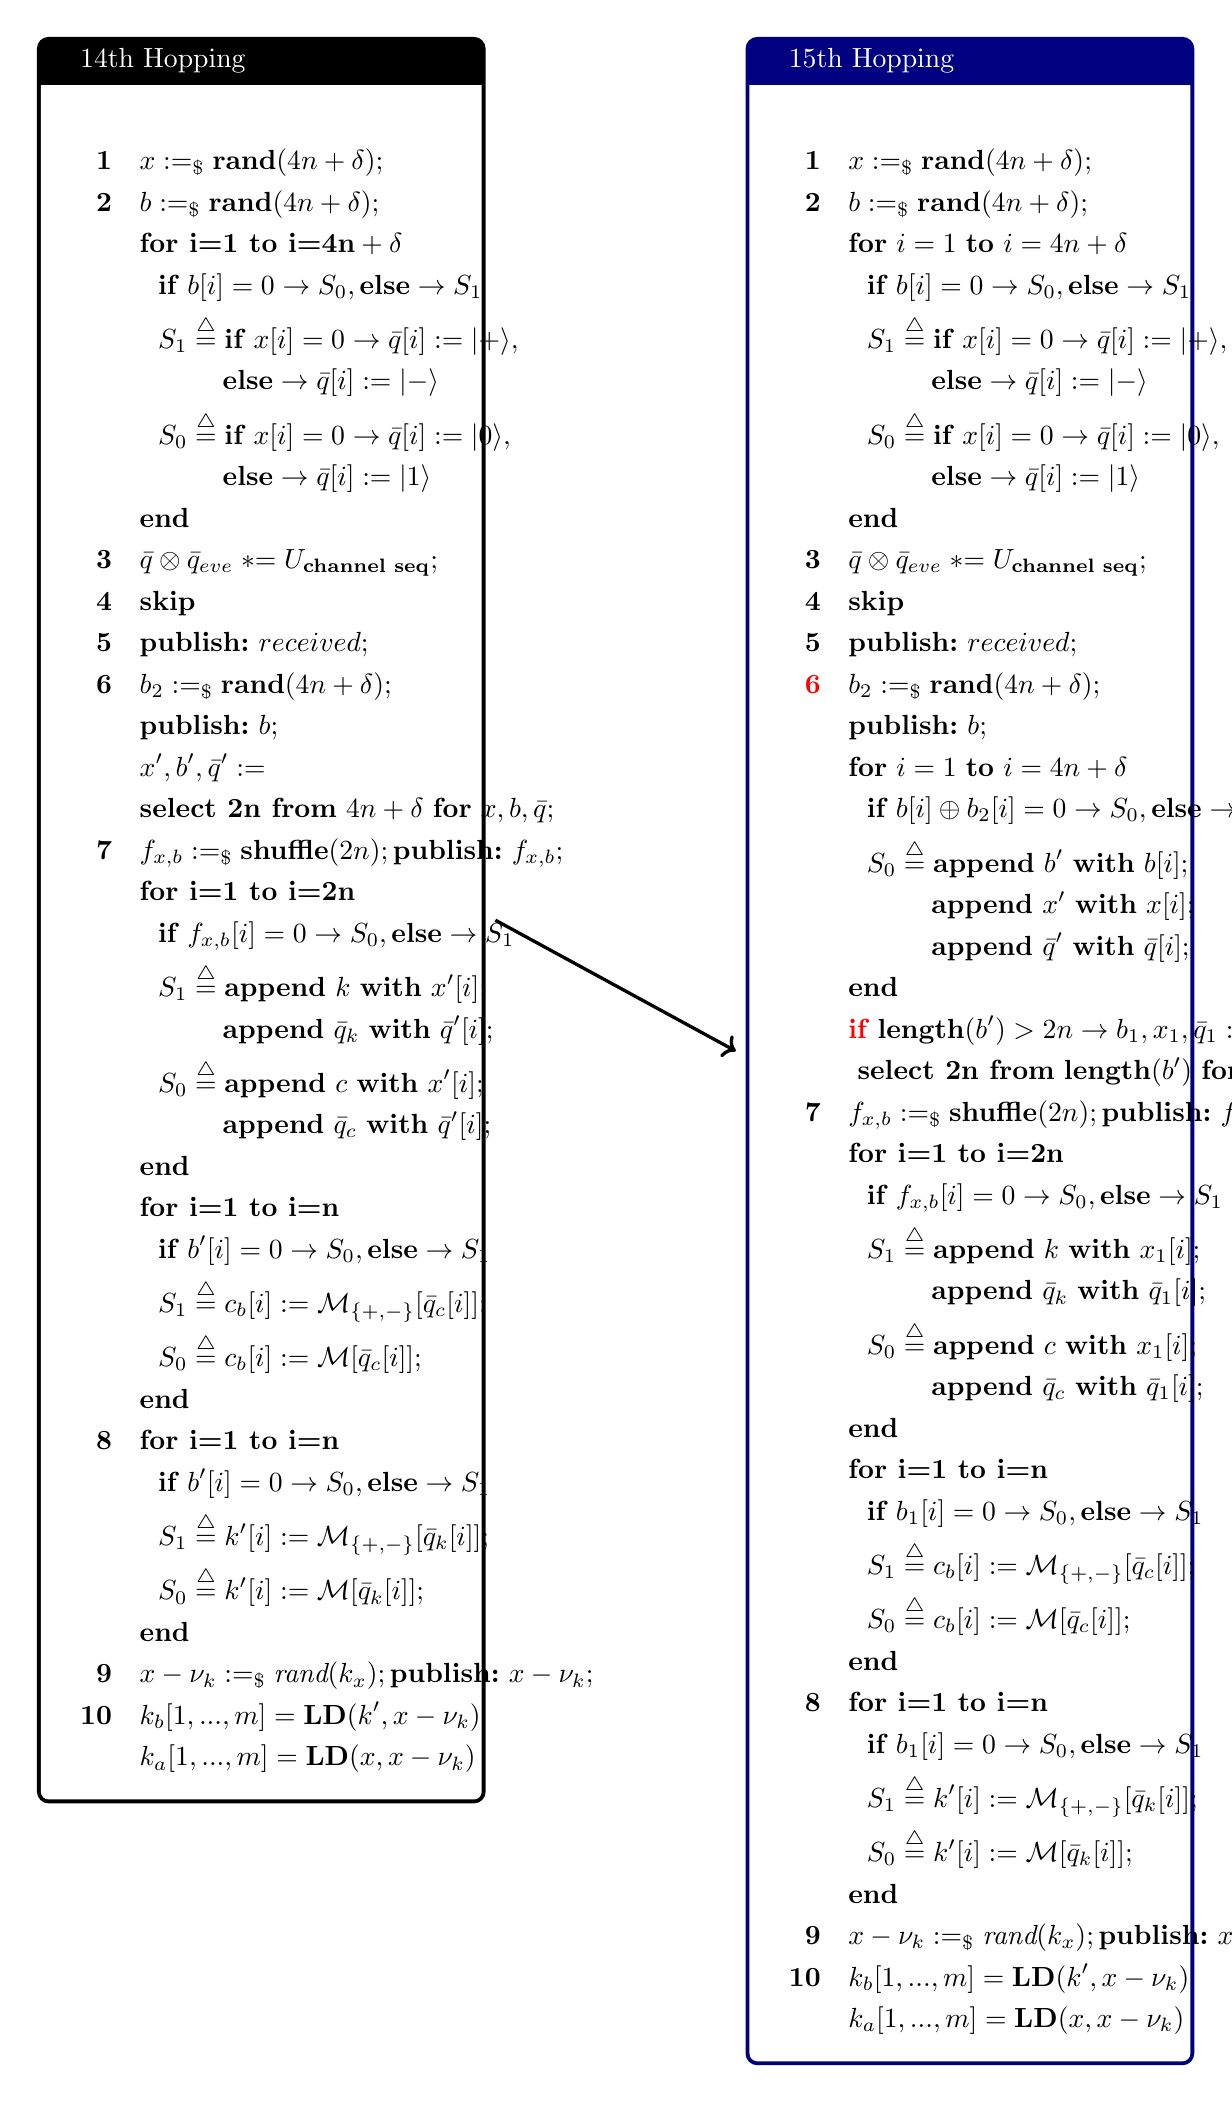
\begin{tikzpicture}[remember picture]

% Left box
\node[anchor=north west] (leftbox) at (0,0) {
\begin{minipage}[t]{0.47\textwidth}
\begin{tcolorbox}[colframe=black!50!black, colback=white, title=14th Hopping, width=\textwidth]
\begin{align*}
    \textbf{{1}} \quad 
    & x :=_\$ \textbf{rand}(4n+\delta); \\ 
    \textbf{{2}}\quad 
    & b :=_\$ \textbf{rand}(4n+\delta); \\
    &\textbf{for i=1 to i=4n}+\delta\\
    &~~ \textbf{if }  b[i] = 0 \rightarrow S_{0} ,\textbf{else}\rightarrow S_{1}\\
    &~~ S_{1}\stackrel{\triangle}{=}\textbf{if }  x[i] = 0 \rightarrow \bar{q}[i] := |+\rangle,\\ &~~~~~~~~~\textbf{else}   \rightarrow \bar{q}[i] := |-\rangle\\
    &~~ S_{0}\stackrel{\triangle}{=}\textbf{if }  x[i] = 0 \rightarrow \bar{q}[i] := |0\rangle,\\ &~~~~~~~~~\textbf{else}   \rightarrow \bar{q}[i] := |1\rangle\\
    &\textbf{end}\\
    \textbf{{3}} 
    \quad & \bar{q} \otimes \bar{q}_{eve} \asteq U_{\textbf{channel seq}}; \\
    \textbf{{4}} \quad &\textbf{skip} \\ 
    \textbf{{5}} \quad & \textbf{publish:}~ received;\\
    \textbf{{6}} \quad & b_2 :=_\$ \textbf{rand}(4n+\delta); \\ \quad & \textbf{publish:}~b;\\
     &x',b',\bar{q}':=\\&\textbf{select 2n from}~4n+\delta ~\textbf{for}~ x,b,\bar{q};\\
    \textbf{{7}} 
    \quad & f_{x,b}:=_\$\textbf{shuffle}(2n); \textbf{publish:}~ f_{x,b};\\
    &\textbf{for i=1  to i=2n}\\
    &~~ \textbf{if }  f_{x,b}[i] = 0 \rightarrow S_{0} ,\textbf{else}\rightarrow S_{1}\\
    &~~ S_{1}\stackrel{\triangle}{=}\textbf{append}~k~\textbf{with}~x'[i];\\
    &~~~~~~~~~\textbf{append}~\bar{q}_k~\textbf{with}~\bar{q}'[i];\\
    &~~ S_{0}\stackrel{\triangle}{=}\textbf{append}~c~\textbf{with}~x'[i];\\
    &~~~~~~~~~\textbf{append}~\bar{q}_c~\textbf{with}~\bar{q}'[i];\\
    &\textbf{end}\\
    &\textbf{for i=1 to i=n}\\
    &~~ \textbf{if }  b'[i] = 0 \rightarrow S_{0} ,\textbf{else}\rightarrow S_{1}\\
    &~~ S_{1}\stackrel{\triangle}{=}c_b[i]:= \mathcal{M}_{\{+,-\}} [\bar{q}_c[i]];\\
    &~~ S_{0}\stackrel{\triangle}{=}c_b[i]:= \mathcal{M} [\bar{q}_c[i]];\\
    &\textbf{end}\\
    \textbf{{8}}\quad 
    &\textbf{for i=1 to i=n}\\
    &~~ \textbf{if }  b'[i] = 0 \rightarrow S_{0} ,\textbf{else}\rightarrow S_{1}\\
    &~~ S_{1}\stackrel{\triangle}{=}k'[i]:= \mathcal{M}_{\{+,-\}} [\bar{q}_k[i]];\\
    &~~ S_{0}\stackrel{\triangle}{=}k'[i]:= \mathcal{M} [\bar{q}_k[i]];\\
    &\textbf{end}\\
    \textbf{{9}} \quad & x-\nu_k :=_\$ \textit{rand}(k_x); \textbf{publish:}~ x-\nu_k;\\
    \textbf{{10}} \quad 
    &k_b[1,...,m]=\textbf{LD}(k',x-\nu_k)\\
    &k_a[1,...,m]=\textbf{LD}(x,x-\nu_k)
\end{align*}
\end{tcolorbox}
\end{minipage}
};

% Right box
\node[anchor=north west] (rightbox) at (9,0) {
\begin{minipage}[t]{0.47\textwidth}
\begin{tcolorbox}[colframe=blue!50!black, colback=white, title=15th Hopping, width=\textwidth]
\begin{align*}
    \textbf{{1}} \quad 
    &x :=_\$ \textbf{rand}(4n+\delta); \\ 
    \textbf{{2}}\quad 
    & b :=_\$ \textbf{rand}(4n+\delta); \\
    &\textbf{for} ~i=1 ~\textbf{to}~ i=4n+\delta\\
    &~~ \textbf{if }  b[i] = 0 \rightarrow S_{0} ,\textbf{else}\rightarrow S_{1}\\
    &~~ S_{1}\stackrel{\triangle}{=}\textbf{if }  x[i] = 0 \rightarrow \bar{q}[i] := |+\rangle,\\ &~~~~~~~~~\textbf{else}   \rightarrow \bar{q}[i] := |-\rangle\\
    &~~ S_{0}\stackrel{\triangle}{=}\textbf{if }  x[i] = 0 \rightarrow \bar{q}[i] := |0\rangle,\\ &~~~~~~~~~\textbf{else}   \rightarrow \bar{q}[i] := |1\rangle\\
    &\textbf{end}\\
    \textbf{{3}} 
    \quad & \bar{q}\otimes \bar{q}_{eve} \asteq U_{\textbf{channel seq}}; \\
    \textbf{{4}} \quad &\textbf{skip} \\ 
    \textbf{{5}} \quad & \textbf{publish:}~ received;\\
    \textbf{\textcolor{red}{6}} \quad & b_2 :=_\$ \textbf{rand}(4n+\delta); \\
    \quad 
    &\textbf{publish:}~ b;\\
    &\textbf{for} ~i=1 ~\textbf{to} ~i=4n+\delta\\
    &~~ \textbf{if } b[i]\oplus b_2[i]=0 \rightarrow S_{0},\textbf{else}\rightarrow\textbf{skip}~, \\
    &~~ S_{0}\stackrel{\triangle}{=}\textbf{append}~b'~\textbf{with}~b[i];\\
    &~~~~~~~~~\textbf{append}~x'~\textbf{with}~x[i];\\
    &~~~~~~~~~\textbf{append}~\bar{q}'~\textbf{with}~\bar{q}[i];\\
    &\textbf{end}\\
    &\textcolor{red}{\textbf{if }} \textbf{length} (b')> 2n\rightarrow b_1,x_1,\bar{q}_1:=\\&~\textbf{select 2n from}~\textbf{length}(b')~\textbf{for}~b',x',\bar{q}';\\
    \textbf{{7}} 
    \quad & f_{x,b}:=_\$\textbf{shuffle}(2n); \textbf{publish:}~ f_{x,b};\\
    &\textbf{for i=1  to i=2n}\\
    &~~ \textbf{if }  f_{x,b}[i] = 0 \rightarrow S_{0} ,\textbf{else}\rightarrow S_{1}\\
    &~~ S_{1}\stackrel{\triangle}{=}\textbf{append}~k~\textbf{with}~x_1[i];\\
    &~~~~~~~~~\textbf{append}~\bar{q}_k~\textbf{with}~\bar{q}_1[i];\\
    &~~ S_{0}\stackrel{\triangle}{=}\textbf{append}~c~\textbf{with}~x_1[i];\\
    &~~~~~~~~~\textbf{append}~\bar{q}_c~\textbf{with}~\bar{q}_1[i];\\
    &\textbf{end}\\
    &\textbf{for i=1 to i=n}\\
    &~~ \textbf{if }  b_1[i] = 0 \rightarrow S_{0} ,\textbf{else}\rightarrow S_{1}\\
    &~~ S_{1}\stackrel{\triangle}{=}c_b[i]:= \mathcal{M}_{\{+,-\}} [\bar{q}_c[i]];\\
    &~~ S_{0}\stackrel{\triangle}{=}c_b[i]:= \mathcal{M} [\bar{q}_c[i]];\\
    &\textbf{end}\\
    \textbf{{8}}\quad 
    &\textbf{for i=1 to i=n}\\
    &~~ \textbf{if }  b_1[i] = 0 \rightarrow S_{0} ,\textbf{else}\rightarrow S_{1}\\
    &~~ S_{1}\stackrel{\triangle}{=}k'[i]:= \mathcal{M}_{\{+,-\}} [\bar{q}_k[i]];\\
    &~~ S_{0}\stackrel{\triangle}{=}k'[i]:= \mathcal{M} [\bar{q}_k[i]];\\
    &\textbf{end}\\
    \textbf{{9}} \quad & x-\nu_k :=_\$ \textit{rand}(k_x); \textbf{publish:}~ x-\nu_k;\\
    \textbf{{10}} \quad 
    &k_b[1,...,m]=\textbf{LD}(k',x-\nu_k)\\
    &k_a[1,...,m]=\textbf{LD}(x,x-\nu_k)
\end{align*}
\end{tcolorbox}
\end{minipage}
};

% Draw arrow between boxes
\draw[->, very thick] (leftbox.east) -- node[above]{} (rightbox.west);

\end{tikzpicture}
\newpage

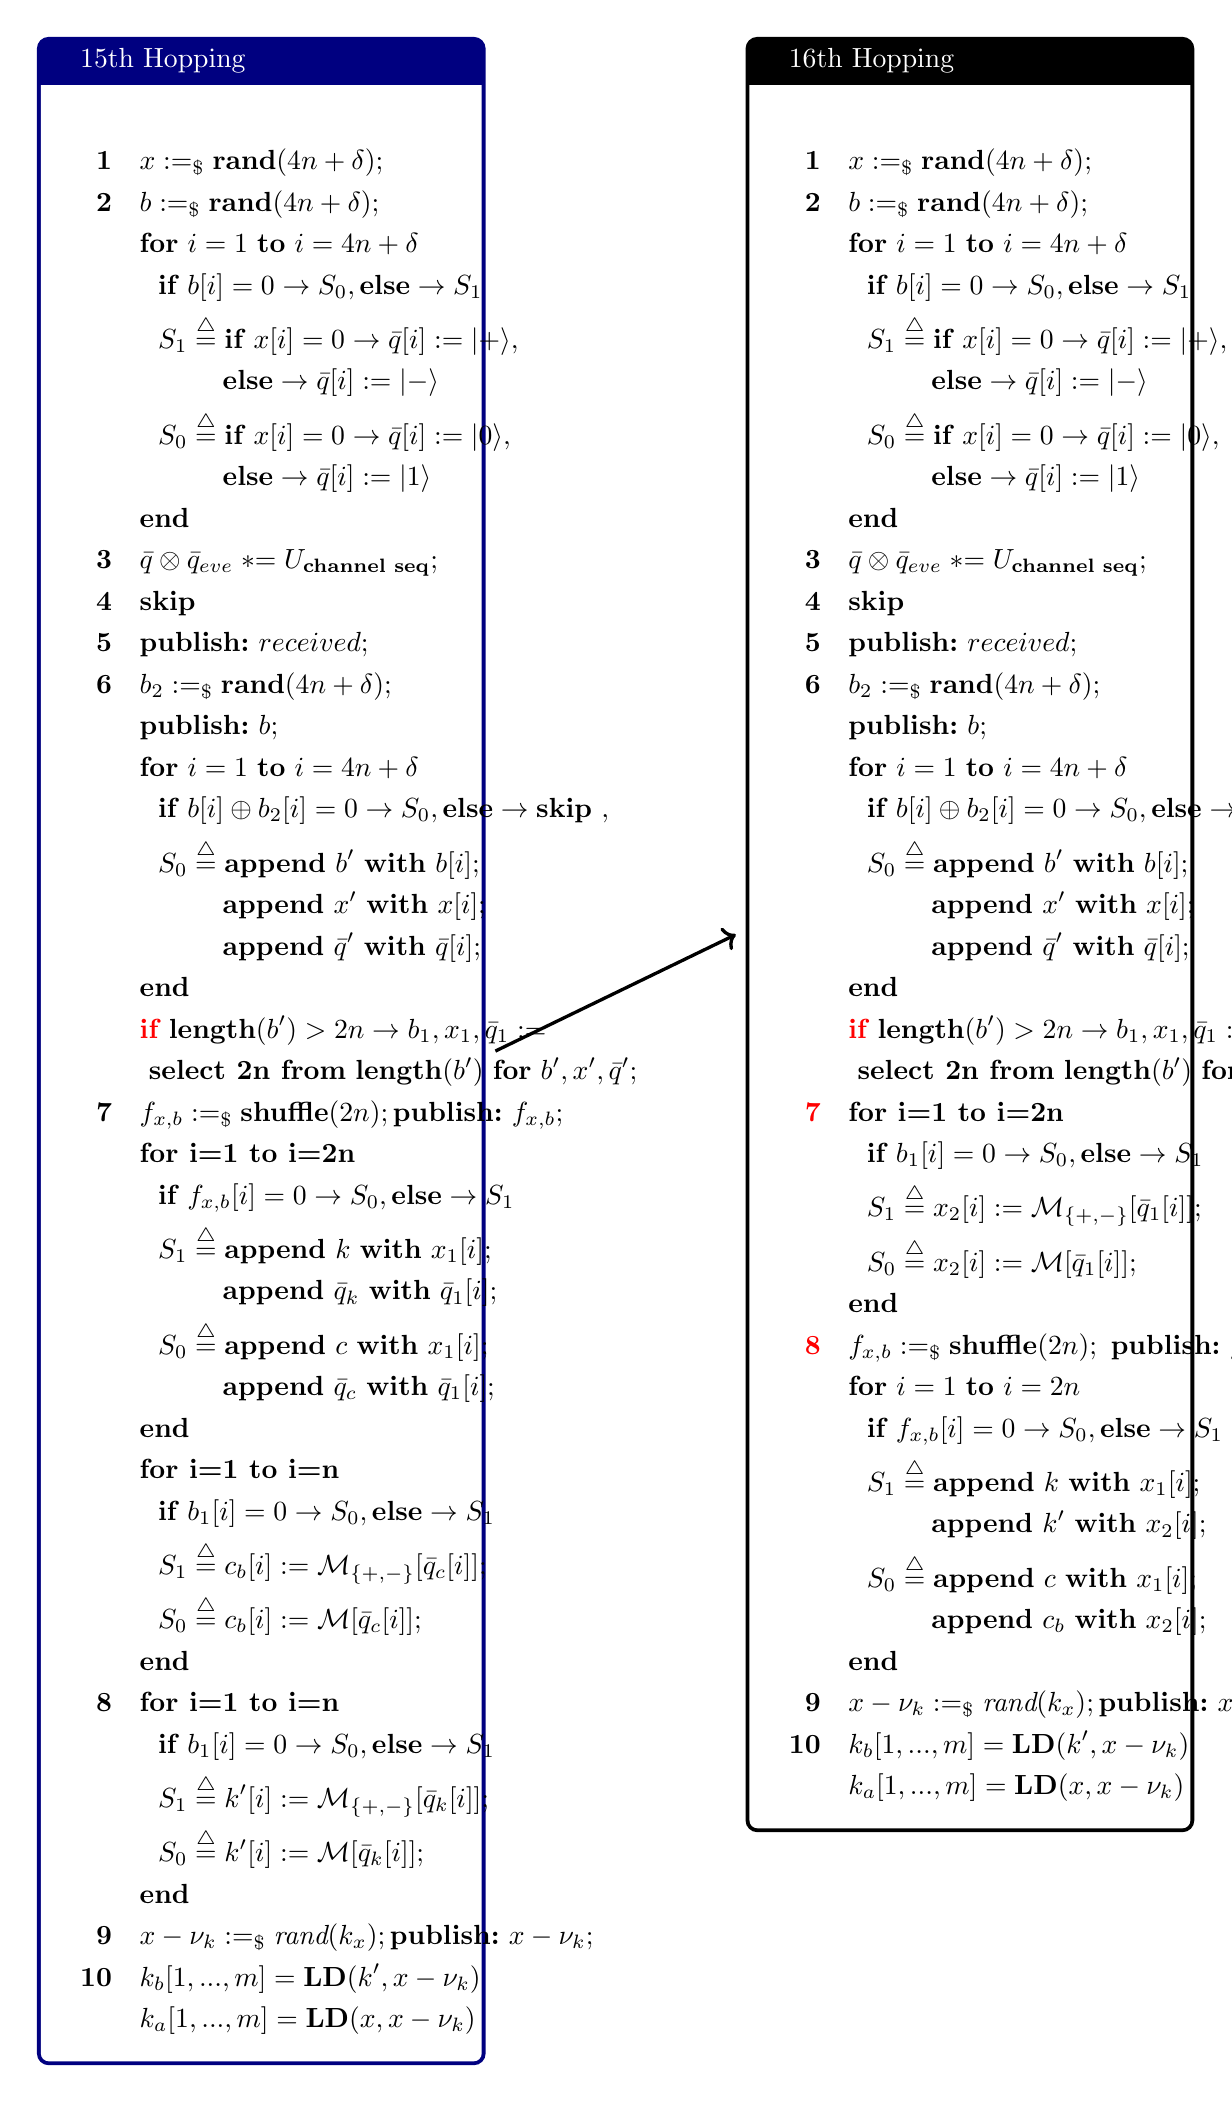
\begin{tikzpicture}[remember picture]

% Left box
\node[anchor=north west] (leftbox) at (0,0) {
\begin{minipage}[t]{0.47\textwidth}
\begin{tcolorbox}[colframe=blue!50!black, colback=white, title=15th Hopping, width=\textwidth]
\begin{align*}
    \textbf{{1}} \quad 
    &x :=_\$ \textbf{rand}(4n+\delta); \\ 
    \textbf{{2}}\quad 
    & b :=_\$ \textbf{rand}(4n+\delta); \\
    &\textbf{for} ~i=1 ~\textbf{to}~ i=4n+\delta\\
    &~~ \textbf{if }  b[i] = 0 \rightarrow S_{0} ,\textbf{else}\rightarrow S_{1}\\
    &~~ S_{1}\stackrel{\triangle}{=}\textbf{if }  x[i] = 0 \rightarrow \bar{q}[i] := |+\rangle,\\ &~~~~~~~~~\textbf{else}   \rightarrow \bar{q}[i] := |-\rangle\\
    &~~ S_{0}\stackrel{\triangle}{=}\textbf{if }  x[i] = 0 \rightarrow \bar{q}[i] := |0\rangle,\\ &~~~~~~~~~\textbf{else}   \rightarrow \bar{q}[i] := |1\rangle\\
    &\textbf{end}\\
    \textbf{{3}} 
    \quad & \bar{q}\otimes \bar{q}_{eve} \asteq U_{\textbf{channel seq}}; \\
    \textbf{{4}} \quad &\textbf{skip} \\ 
    \textbf{{5}} \quad & \textbf{publish:}~ received;\\
    \textbf{{6}} \quad & b_2 :=_\$ \textbf{rand}(4n+\delta); \\
    \quad 
    &\textbf{publish:}~ b;\\
    &\textbf{for} ~i=1 ~\textbf{to} ~i=4n+\delta\\
    &~~ \textbf{if } b[i]\oplus b_2[i]=0 \rightarrow S_{0},\textbf{else}\rightarrow\textbf{skip}~, \\
    &~~ S_{0}\stackrel{\triangle}{=}\textbf{append}~b'~\textbf{with}~b[i];\\
    &~~~~~~~~~\textbf{append}~x'~\textbf{with}~x[i];\\
    &~~~~~~~~~\textbf{append}~\bar{q}'~\textbf{with}~\bar{q}[i];\\
    &\textbf{end}\\
    &\textcolor{red}{\textbf{if }} \textbf{length} (b')> 2n\rightarrow b_1,x_1,\bar{q}_1:=\\&~\textbf{select 2n from}~\textbf{length}(b')~\textbf{for}~b',x',\bar{q}';\\
    \textbf{{7}} 
    \quad & f_{x,b}:=_\$\textbf{shuffle}(2n); \textbf{publish:}~ f_{x,b};\\
    &\textbf{for i=1  to i=2n}\\
    &~~ \textbf{if }  f_{x,b}[i] = 0 \rightarrow S_{0} ,\textbf{else}\rightarrow S_{1}\\
    &~~ S_{1}\stackrel{\triangle}{=}\textbf{append}~k~\textbf{with}~x_1[i];\\
    &~~~~~~~~~\textbf{append}~\bar{q}_k~\textbf{with}~\bar{q}_1[i];\\
    &~~ S_{0}\stackrel{\triangle}{=}\textbf{append}~c~\textbf{with}~x_1[i];\\
    &~~~~~~~~~\textbf{append}~\bar{q}_c~\textbf{with}~\bar{q}_1[i];\\
    &\textbf{end}\\
    &\textbf{for i=1 to i=n}\\
    &~~ \textbf{if }  b_1[i] = 0 \rightarrow S_{0} ,\textbf{else}\rightarrow S_{1}\\
    &~~ S_{1}\stackrel{\triangle}{=}c_b[i]:= \mathcal{M}_{\{+,-\}} [\bar{q}_c[i]];\\
    &~~ S_{0}\stackrel{\triangle}{=}c_b[i]:= \mathcal{M} [\bar{q}_c[i]];\\
    &\textbf{end}\\
    \textbf{{8}}\quad 
    &\textbf{for i=1 to i=n}\\
    &~~ \textbf{if }  b_1[i] = 0 \rightarrow S_{0} ,\textbf{else}\rightarrow S_{1}\\
    &~~ S_{1}\stackrel{\triangle}{=}k'[i]:= \mathcal{M}_{\{+,-\}} [\bar{q}_k[i]];\\
    &~~ S_{0}\stackrel{\triangle}{=}k'[i]:= \mathcal{M} [\bar{q}_k[i]];\\
    &\textbf{end}\\
    \textbf{{9}} \quad & x-\nu_k :=_\$ \textit{rand}(k_x); \textbf{publish:}~ x-\nu_k;\\
    \textbf{{10}} \quad 
    &k_b[1,...,m]=\textbf{LD}(k',x-\nu_k)\\
    &k_a[1,...,m]=\textbf{LD}(x,x-\nu_k)
\end{align*}
\end{tcolorbox}
\end{minipage}
};

% Right box
\node[anchor=north west] (rightbox) at (9,0) {
\begin{minipage}[t]{0.47\textwidth}
\begin{tcolorbox}[colframe=black!50!black, colback=white, title=16th Hopping, width=\textwidth]
\begin{align*}
    \textbf{{1}} \quad 
    & x :=_\$ \textbf{rand}(4n+\delta); \\ 
    \textbf{{2}}\quad 
    & b :=_\$ \textbf{rand}(4n+\delta); \\
    &\textbf{for} ~i=1 ~\textbf{to}~ i=4n+\delta\\
    &~~ \textbf{if }  b[i] = 0 \rightarrow S_{0} ,\textbf{else}\rightarrow S_{1}\\
    &~~ S_{1}\stackrel{\triangle}{=}\textbf{if }  x[i] = 0 \rightarrow \bar{q}[i] := |+\rangle,\\ &~~~~~~~~~\textbf{else}   \rightarrow \bar{q}[i] := |-\rangle\\
    &~~ S_{0}\stackrel{\triangle}{=}\textbf{if }  x[i] = 0 \rightarrow \bar{q}[i] := |0\rangle,\\ &~~~~~~~~~\textbf{else}   \rightarrow \bar{q}[i] := |1\rangle\\
    &\textbf{end}\\
    \textbf{{3}} 
    \quad & \bar{q}\otimes \bar{q}_{eve} \asteq U_{\textbf{channel seq}}; \\
    \textbf{{4}} \quad &\textbf{skip} \\ 
    \textbf{{5}} \quad & \textbf{publish:}~ received;\\
    \textbf{{6}} \quad & b_2 :=_\$ \textbf{rand}(4n+\delta); \\
    \quad 
    &\textbf{publish:}~ b;\\
    &\textbf{for} ~i=1 ~\textbf{to} ~i=4n+\delta\\
    &~~ \textbf{if } b[i]\oplus b_2[i]=0 \rightarrow S_{0},\textbf{else}\rightarrow\textbf{skip}~, \\
    &~~ S_{0}\stackrel{\triangle}{=}\textbf{append}~b'~\textbf{with}~b[i];\\
    &~~~~~~~~~\textbf{append}~x'~\textbf{with}~x[i];\\
    &~~~~~~~~~\textbf{append}~\bar{q}'~\textbf{with}~\bar{q}[i];\\
    &\textbf{end}\\
    &\textcolor{red}{\textbf{if }} \textbf{length} (b')> 2n\rightarrow b_1,x_1,\bar{q}_1:=\\&~\textbf{select 2n from}~\textbf{length}(b')~\textbf{for}~b',x',\bar{q}';\\
    \textbf{\textcolor{red}{7}} 
    \quad 
    &\textbf{for i=1 to i=2n}\\
    &~~ \textbf{if }  b_1[i] = 0 \rightarrow S_{0} ,\textbf{else}\rightarrow S_{1}\\
    &~~ S_{1}\stackrel{\triangle}{=}x_2[i]:= \mathcal{M}_{\{+,-\}} [\bar{q}_1[i]];\\
    &~~ S_{0}\stackrel{\triangle}{=}x_2[i]:= \mathcal{M} [\bar{q}_1[i]];\\
    &\textbf{end}\\
    \textbf{\textcolor{red}{8}}\quad &f_{x,b}:=_\$\textbf{shuffle}(2n); ~\textbf{publish:}~f_{x,b};\\
    &\textbf{for} ~i=1 ~\textbf{to} ~i=2n\\
    &~~ \textbf{if }  f_{x,b}[i] = 0 \rightarrow S_{0} ,\textbf{else}\rightarrow S_{1}\\
    &~~ S_{1}\stackrel{\triangle}{=}\textbf{append}~k~\textbf{with}~x_1[i];\\
    &~~~~~~~~~\textbf{append}~k'~\textbf{with}~x_2[i];\\
    &~~ S_{0}\stackrel{\triangle}{=}\textbf{append}~c~\textbf{with}~x_1[i];\\
    &~~~~~~~~~\textbf{append}~c_b~\textbf{with}~x_2[i];\\
    &\textbf{end}\\
    \textbf{{9}} \quad & x-\nu_k :=_\$ \textit{rand}(k_x); \textbf{publish:}~ x-\nu_k;\\
    \textbf{{10}} \quad 
    &k_b[1,...,m]=\textbf{LD}(k',x-\nu_k)\\
    &k_a[1,...,m]=\textbf{LD}(x,x-\nu_k)
\end{align*}
\end{tcolorbox}
\end{minipage}
};

% Draw arrow between boxes
\draw[->, very thick] (leftbox.east) -- node[above]{} (rightbox.west);

\end{tikzpicture}
\newpage

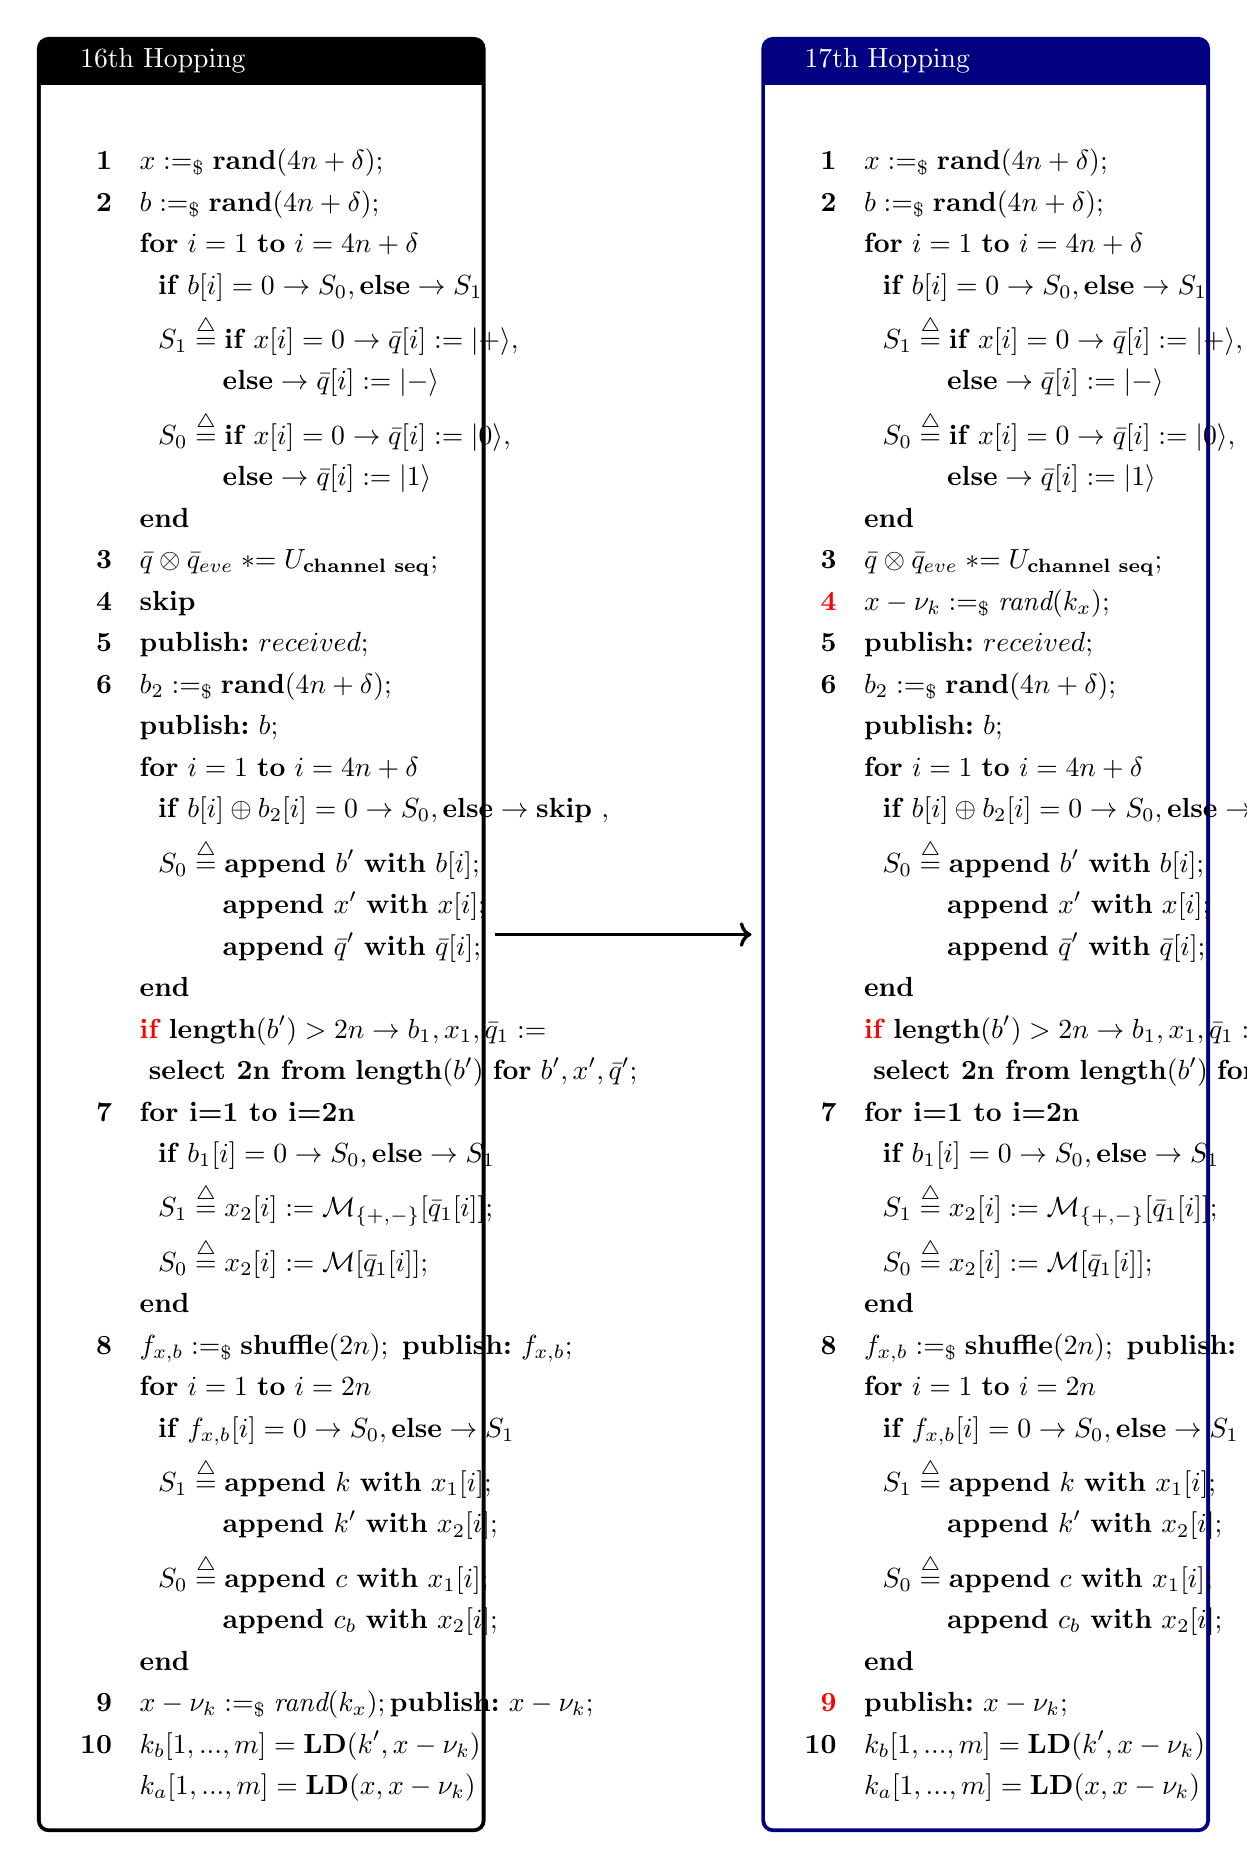
\begin{tikzpicture}[remember picture]

% Left box
\node[anchor=north west] (leftbox) at (0,0) {
\begin{minipage}[t]{0.47\textwidth}
\begin{tcolorbox}[colframe=black!50!black, colback=white, title=16th Hopping, width=\textwidth]
\begin{align*}
    \textbf{{1}} \quad 
    & x :=_\$ \textbf{rand}(4n+\delta); \\ 
    \textbf{{2}}\quad 
    & b :=_\$ \textbf{rand}(4n+\delta); \\
    &\textbf{for} ~i=1 ~\textbf{to}~ i=4n+\delta\\
    &~~ \textbf{if }  b[i] = 0 \rightarrow S_{0} ,\textbf{else}\rightarrow S_{1}\\
    &~~ S_{1}\stackrel{\triangle}{=}\textbf{if }  x[i] = 0 \rightarrow \bar{q}[i] := |+\rangle,\\ &~~~~~~~~~\textbf{else}   \rightarrow \bar{q}[i] := |-\rangle\\
    &~~ S_{0}\stackrel{\triangle}{=}\textbf{if }  x[i] = 0 \rightarrow \bar{q}[i] := |0\rangle,\\ &~~~~~~~~~\textbf{else}   \rightarrow \bar{q}[i] := |1\rangle\\
    &\textbf{end}\\
    \textbf{{3}} 
    \quad & \bar{q}\otimes \bar{q}_{eve} \asteq U_{\textbf{channel seq}}; \\
    \textbf{{4}} \quad &\textbf{skip} \\ 
    \textbf{{5}} \quad & \textbf{publish:}~ received;\\
    \textbf{{6}} \quad & b_2 :=_\$ \textbf{rand}(4n+\delta); \\
    \quad 
    &\textbf{publish:}~ b;\\
    &\textbf{for} ~i=1 ~\textbf{to} ~i=4n+\delta\\
    &~~ \textbf{if } b[i]\oplus b_2[i]=0 \rightarrow S_{0},\textbf{else}\rightarrow\textbf{skip}~, \\
    &~~ S_{0}\stackrel{\triangle}{=}\textbf{append}~b'~\textbf{with}~b[i];\\
    &~~~~~~~~~\textbf{append}~x'~\textbf{with}~x[i];\\
    &~~~~~~~~~\textbf{append}~\bar{q}'~\textbf{with}~\bar{q}[i];\\
    &\textbf{end}\\
    &\textcolor{red}{\textbf{if } }\textbf{length} (b')> 2n\rightarrow b_1,x_1,\bar{q}_1:=\\&~\textbf{select 2n from}~\textbf{length}(b')~\textbf{for}~b',x',\bar{q}';\\
    \textbf{{7}} 
    \quad 
    &\textbf{for i=1 to i=2n}\\
    &~~ \textbf{if }  b_1[i] = 0 \rightarrow S_{0} ,\textbf{else}\rightarrow S_{1}\\
    &~~ S_{1}\stackrel{\triangle}{=}x_2[i]:= \mathcal{M}_{\{+,-\}} [\bar{q}_1[i]];\\
    &~~ S_{0}\stackrel{\triangle}{=}x_2[i]:= \mathcal{M} [\bar{q}_1[i]];\\
    &\textbf{end}\\
    \textbf{{8}}\quad &f_{x,b}:=_\$\textbf{shuffle}(2n); ~\textbf{publish:}~f_{x,b};\\
    &\textbf{for} ~i=1 ~\textbf{to} ~i=2n\\
    &~~ \textbf{if }  f_{x,b}[i] = 0 \rightarrow S_{0} ,\textbf{else}\rightarrow S_{1}\\
    &~~ S_{1}\stackrel{\triangle}{=}\textbf{append}~k~\textbf{with}~x_1[i];\\
    &~~~~~~~~~\textbf{append}~k'~\textbf{with}~x_2[i];\\
    &~~ S_{0}\stackrel{\triangle}{=}\textbf{append}~c~\textbf{with}~x_1[i];\\
    &~~~~~~~~~\textbf{append}~c_b~\textbf{with}~x_2[i];\\
    &\textbf{end}\\
    \textbf{{9}} \quad & x-\nu_k :=_\$ \textit{rand}(k_x); \textbf{publish:}~ x-\nu_k;\\
    \textbf{{10}} \quad 
    &k_b[1,...,m]=\textbf{LD}(k',x-\nu_k)\\
    &k_a[1,...,m]=\textbf{LD}(x,x-\nu_k)
\end{align*}
\end{tcolorbox}
\end{minipage}
};

% Right box
\node[anchor=north west] (rightbox) at (9.2,0) {
\begin{minipage}[t]{0.47\textwidth}
\begin{tcolorbox}[colframe=blue!50!black, colback=white, title=17th Hopping, width=\textwidth]
\begin{align*}
    \textbf{{1}} \quad 
    & x :=_\$ \textbf{rand}(4n+\delta); \\ 
    \textbf{{2}}\quad 
    & b :=_\$ \textbf{rand}(4n+\delta); \\
    &\textbf{for} ~i=1 ~\textbf{to}~ i=4n+\delta\\
    &~~ \textbf{if }  b[i] = 0 \rightarrow S_{0} ,\textbf{else}\rightarrow S_{1}\\
    &~~ S_{1}\stackrel{\triangle}{=}\textbf{if }  x[i] = 0 \rightarrow \bar{q}[i] := |+\rangle,\\ &~~~~~~~~~\textbf{else}   \rightarrow \bar{q}[i] := |-\rangle\\
    &~~ S_{0}\stackrel{\triangle}{=}\textbf{if }  x[i] = 0 \rightarrow \bar{q}[i] := |0\rangle,\\ &~~~~~~~~~\textbf{else}   \rightarrow \bar{q}[i] := |1\rangle\\
    &\textbf{end}\\
    \textbf{{3}} 
    \quad & \bar{q}\otimes \bar{q}_{eve} \asteq U_{\textbf{channel seq}}; \\
    \textbf{\textcolor{red}{4}} \quad & x-\nu_k :=_\$ \textit{rand}(k_x); \\ 
    \textbf{{5}} \quad & \textbf{publish:}~ received;\\
    \textbf{{6}} \quad & b_2 :=_\$ \textbf{rand}(4n+\delta); \\
    \quad 
    &\textbf{publish:}~ b;\\
    &\textbf{for} ~i=1 ~\textbf{to} ~i=4n+\delta\\
    &~~ \textbf{if } b[i]\oplus b_2[i]=0 \rightarrow S_{0},\textbf{else}\rightarrow\textbf{skip}~, \\
    &~~ S_{0}\stackrel{\triangle}{=}\textbf{append}~b'~\textbf{with}~b[i];\\
    &~~~~~~~~~\textbf{append}~x'~\textbf{with}~x[i];\\
    &~~~~~~~~~\textbf{append}~\bar{q}'~\textbf{with}~\bar{q}[i];\\
    &\textbf{end}\\
    &\textcolor{red}{\textbf{if } }\textbf{length} (b')> 2n\rightarrow b_1,x_1,\bar{q}_1:=\\&~\textbf{select 2n from}~\textbf{length}(b')~\textbf{for}~b',x',\bar{q}';\\
    \textbf{{7}} 
    \quad 
    &\textbf{for i=1 to i=2n}\\
    &~~ \textbf{if }  b_1[i] = 0 \rightarrow S_{0} ,\textbf{else}\rightarrow S_{1}\\
    &~~ S_{1}\stackrel{\triangle}{=}x_2[i]:= \mathcal{M}_{\{+,-\}} [\bar{q}_1[i]];\\
    &~~ S_{0}\stackrel{\triangle}{=}x_2[i]:= \mathcal{M} [\bar{q}_1[i]];\\
    &\textbf{end}\\
    \textbf{{8}}\quad &f_{x,b}:=_\$\textbf{shuffle}(2n); ~\textbf{publish:}~f_{x,b};\\
    &\textbf{for} ~i=1 ~\textbf{to} ~i=2n\\
    &~~ \textbf{if }  f_{x,b}[i] = 0 \rightarrow S_{0} ,\textbf{else}\rightarrow S_{1}\\
    &~~ S_{1}\stackrel{\triangle}{=}\textbf{append}~k~\textbf{with}~x_1[i];\\
    &~~~~~~~~~\textbf{append}~k'~\textbf{with}~x_2[i];\\
    &~~ S_{0}\stackrel{\triangle}{=}\textbf{append}~c~\textbf{with}~x_1[i];\\
    &~~~~~~~~~\textbf{append}~c_b~\textbf{with}~x_2[i];\\
    &\textbf{end}\\
    \textbf{\textcolor{red}{9}} \quad & \textbf{publish:}~ x-\nu_k;\\
    \textbf{{10}} \quad 
    &k_b[1,...,m]=\textbf{LD}(k',x-\nu_k)\\
    &k_a[1,...,m]=\textbf{LD}(x,x-\nu_k)
\end{align*}
\end{tcolorbox}
\end{minipage}
};

% Draw arrow between boxes
\draw[->, very thick] (leftbox.east) -- node[above]{} (rightbox.west);

\end{tikzpicture}
\newpage


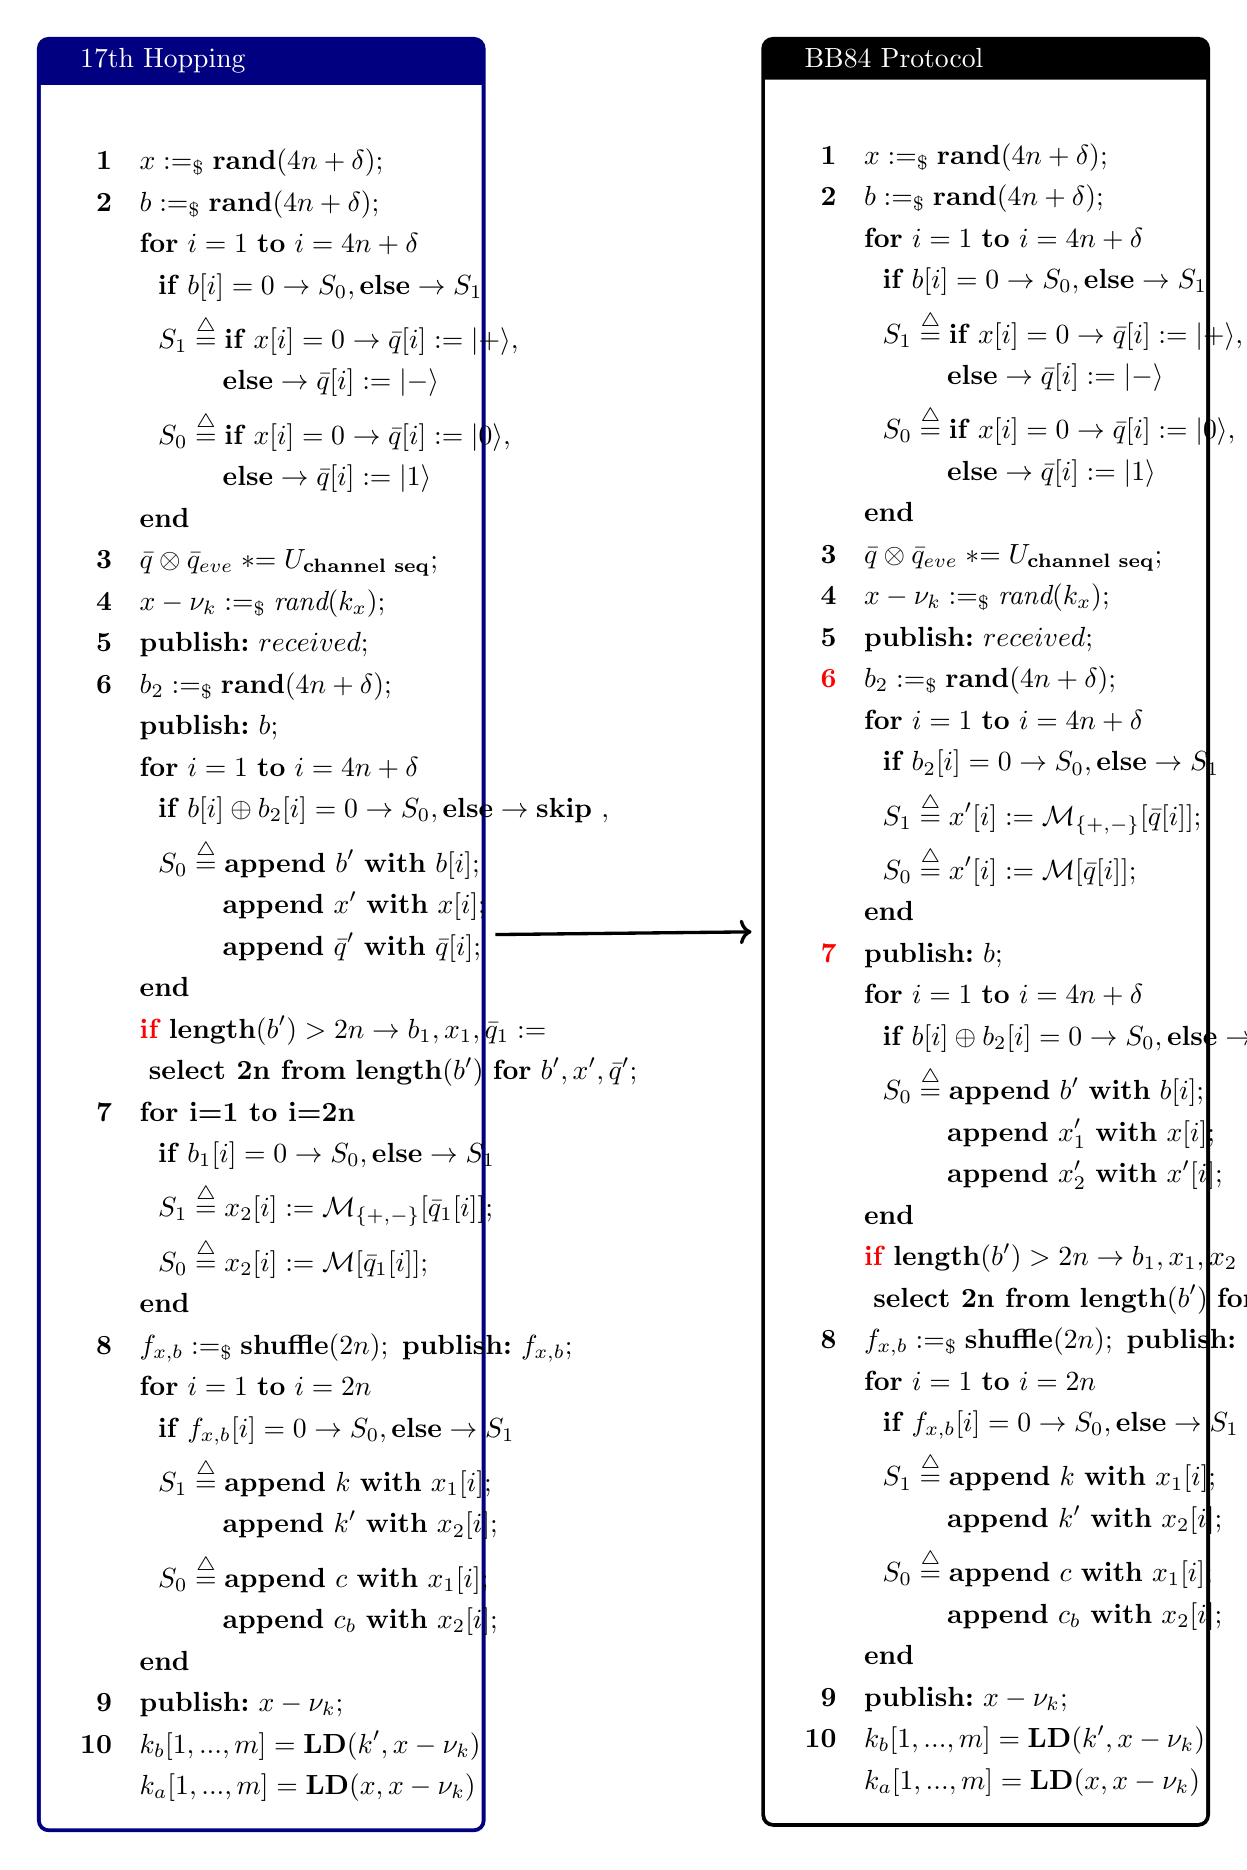
\begin{tikzpicture}[remember picture]

% Left box
\node[anchor=north west] (leftbox) at (0,0) {
\begin{minipage}[t]{0.47\textwidth}
\begin{tcolorbox}[colframe=blue!50!black, colback=white, title=17th Hopping, width=\textwidth]
\begin{align*}
    \textbf{{1}} \quad 
    & x :=_\$ \textbf{rand}(4n+\delta); \\ 
    \textbf{{2}}\quad 
    & b :=_\$ \textbf{rand}(4n+\delta); \\
    &\textbf{for} ~i=1 ~\textbf{to}~ i=4n+\delta\\
    &~~ \textbf{if }  b[i] = 0 \rightarrow S_{0} ,\textbf{else}\rightarrow S_{1}\\
    &~~ S_{1}\stackrel{\triangle}{=}\textbf{if }  x[i] = 0 \rightarrow \bar{q}[i] := |+\rangle,\\ &~~~~~~~~~\textbf{else}   \rightarrow \bar{q}[i] := |-\rangle\\
    &~~ S_{0}\stackrel{\triangle}{=}\textbf{if }  x[i] = 0 \rightarrow \bar{q}[i] := |0\rangle,\\ &~~~~~~~~~\textbf{else}   \rightarrow \bar{q}[i] := |1\rangle\\
    &\textbf{end}\\
    \textbf{{3}} 
    \quad & \bar{q}\otimes \bar{q}_{eve} \asteq U_{\textbf{channel seq}}; \\
    \textbf{{4}} \quad & x-\nu_k :=_\$ \textit{rand}(k_x); \\ 
    \textbf{{5}} \quad & \textbf{publish:}~ received;\\
    \textbf{{6}} \quad & b_2 :=_\$ \textbf{rand}(4n+\delta); \\
    \quad 
    &\textbf{publish:}~ b;\\
    &\textbf{for} ~i=1 ~\textbf{to} ~i=4n+\delta\\
    &~~ \textbf{if } b[i]\oplus b_2[i]=0 \rightarrow S_{0},\textbf{else}\rightarrow\textbf{skip}~, \\
    &~~ S_{0}\stackrel{\triangle}{=}\textbf{append}~b'~\textbf{with}~b[i];\\
    &~~~~~~~~~\textbf{append}~x'~\textbf{with}~x[i];\\
    &~~~~~~~~~\textbf{append}~\bar{q}'~\textbf{with}~\bar{q}[i];\\
    &\textbf{end}\\
    &\textcolor{red}{\textbf{if } }\textbf{length} (b')> 2n\rightarrow b_1,x_1,\bar{q}_1:=\\&~\textbf{select 2n from}~\textbf{length}(b')~\textbf{for}~b',x',\bar{q}';\\
    \textbf{{7}} 
    \quad 
    &\textbf{for i=1 to i=2n}\\
    &~~ \textbf{if }  b_1[i] = 0 \rightarrow S_{0} ,\textbf{else}\rightarrow S_{1}\\
    &~~ S_{1}\stackrel{\triangle}{=}x_2[i]:= \mathcal{M}_{\{+,-\}} [\bar{q}_1[i]];\\
    &~~ S_{0}\stackrel{\triangle}{=}x_2[i]:= \mathcal{M} [\bar{q}_1[i]];\\
    &\textbf{end}\\
    \textbf{{8}}\quad &f_{x,b}:=_\$\textbf{shuffle}(2n); ~\textbf{publish:}~f_{x,b};\\
    &\textbf{for} ~i=1 ~\textbf{to} ~i=2n\\
    &~~ \textbf{if }  f_{x,b}[i] = 0 \rightarrow S_{0} ,\textbf{else}\rightarrow S_{1}\\
    &~~ S_{1}\stackrel{\triangle}{=}\textbf{append}~k~\textbf{with}~x_1[i];\\
    &~~~~~~~~~\textbf{append}~k'~\textbf{with}~x_2[i];\\
    &~~ S_{0}\stackrel{\triangle}{=}\textbf{append}~c~\textbf{with}~x_1[i];\\
    &~~~~~~~~~\textbf{append}~c_b~\textbf{with}~x_2[i];\\
    &\textbf{end}\\
    \textbf{{9}} \quad & \textbf{publish:}~ x-\nu_k;\\
    \textbf{{10}} \quad 
    &k_b[1,...,m]=\textbf{LD}(k',x-\nu_k)\\
    &k_a[1,...,m]=\textbf{LD}(x,x-\nu_k)
\end{align*}
\end{tcolorbox}
\end{minipage}
};

% Right box
\node[anchor=north west] (rightbox) at (9.2,0) {
\begin{minipage}[t]{0.47\textwidth}
\begin{tcolorbox}[colframe=black!50!black, colback=white, title=BB84 Protocol, width=\textwidth]
\begin{align*}
    \textbf{{1}} \quad 
    & x :=_\$ \textbf{rand}(4n+\delta); \\ 
    \textbf{{2}}\quad 
    & b :=_\$ \textbf{rand}(4n+\delta); \\
    &\textbf{for} ~i=1 ~\textbf{to}~ i=4n+\delta\\
    &~~ \textbf{if }  b[i] = 0 \rightarrow S_{0} ,\textbf{else}\rightarrow S_{1}\\
    &~~ S_{1}\stackrel{\triangle}{=}\textbf{if }  x[i] = 0 \rightarrow \bar{q}[i] := |+\rangle,\\ &~~~~~~~~~\textbf{else}   \rightarrow \bar{q}[i] := |-\rangle\\
    &~~ S_{0}\stackrel{\triangle}{=}\textbf{if }  x[i] = 0 \rightarrow \bar{q}[i] := |0\rangle,\\ &~~~~~~~~~\textbf{else}   \rightarrow \bar{q}[i] := |1\rangle\\
    &\textbf{end}\\
    \textbf{{3}} 
    \quad & \bar{q}\otimes \bar{q}_{eve} \asteq U_{\textbf{channel seq}}; \\
    \textbf{{4}} \quad & x-\nu_k :=_\$ \textit{rand}(k_x); \\ 
    \textbf{{5}} \quad & \textbf{publish:}~ received;\\
    \textbf{\textcolor{red}{6}} \quad & b_2 :=_\$ \textbf{rand}(4n+\delta); \\
    &\textbf{for} ~i=1 ~\textbf{to} ~i=4n+\delta\\
    &~~ \textbf{if }  b_2[i] = 0 \rightarrow S_{0} ,\textbf{else}\rightarrow S_{1}\\
    &~~ S_{1}\stackrel{\triangle}{=}x'[i]:= \mathcal{M}_{\{+,-\}} [\bar{q}[i]];\\
    &~~ S_{0}\stackrel{\triangle}{=}x'[i]:= \mathcal{M} [\bar{q}[i]];\\
    &\textbf{end}\\
    \textbf{\textcolor{red}{7}} 
    \quad 
    &\textbf{publish:}~ b;\\
    &\textbf{for} ~i=1 ~\textbf{to} ~i=4n+\delta\\
    &~~ \textbf{if } b[i]\oplus b_2[i]=0 \rightarrow S_{0},\textbf{else}\rightarrow\textbf{skip}~, \\
    &~~ S_{0}\stackrel{\triangle}{=}\textbf{append}~b'~\textbf{with}~b[i];\\
    &~~~~~~~~~\textbf{append}~x'_1~\textbf{with}~x[i];\\
    &~~~~~~~~~\textbf{append}~x'_2~\textbf{with}~x'[i];\\
    &\textbf{end}\\
    &\textcolor{red}{\textbf{if }} \textbf{length} (b')> 2n\rightarrow b_1,x_1,x_2:=\\&~\textbf{select 2n from}~\textbf{length}(b')~\textbf{for}~b',x'_1,x'_2;\\
    \textbf{{8}}\quad &f_{x,b}:=_\$\textbf{shuffle}(2n); ~\textbf{publish:}~f_{x,b};\\
    &\textbf{for} ~i=1 ~\textbf{to} ~i=2n\\
    &~~ \textbf{if }  f_{x,b}[i] = 0 \rightarrow S_{0} ,\textbf{else}\rightarrow S_{1}\\
    &~~ S_{1}\stackrel{\triangle}{=}\textbf{append}~k~\textbf{with}~x_1[i];\\
    &~~~~~~~~~\textbf{append}~k'~\textbf{with}~x_2[i];\\
    &~~ S_{0}\stackrel{\triangle}{=}\textbf{append}~c~\textbf{with}~x_1[i];\\
    &~~~~~~~~~\textbf{append}~c_b~\textbf{with}~x_2[i];\\
    &\textbf{end}\\
    \textbf{{9}} \quad & \textbf{publish:}~ x-\nu_k;\\
    \textbf{{10}} \quad 
    &k_b[1,...,m]=\textbf{LD}(k',x-\nu_k)\\
    &k_a[1,...,m]=\textbf{LD}(x,x-\nu_k)
\end{align*}
\end{tcolorbox}
\end{minipage}
};

% Draw arrow between boxes
\draw[->, very thick] (leftbox.east) -- node[above]{} (rightbox.west);

\end{tikzpicture}

\newpage

\chapter{Summarizations}


\subsection{Rules}

\begin{definition}[Variable Names to Address Indexes]
    Ahead of program execution, all variables in it will have fixed indexes. We map variables to addresses like below:
    \[\overset{\textbf{Quantum variables}}{\overbrace{ \bar{q}\rightarrow[1,...,n_q]}}~~~\overset{\textbf{Probability Distributions}}{\overbrace{ p\rightarrow[n_q+1,...,n_q+n_p]}}~~~\overset{\textbf{Classical variables}}{\overbrace{ x\rightarrow[n_q+n_p+1,...,n_q+n_p+n_x]}}\]
\end{definition}

\begin{definition}[Classical-quantum State lifting]
Two c-q states $\triangle =$ $\sum_i \mu_1[i]\ket{i}\bra{i}\otimes \rho_i\ $ (with address indexes $[i_1,...,i_m]$) and $\triangle'=$ $ \sum_j \mu_2[j]\ket{j}\bra{j}\otimes \rho'_j$ (with address indexes $[i'_1,...,i'_m]$), where $\rho_i\in D(\mathcal{H}_1)$ and $\rho'_j\in D(\mathcal{H}_2)$, are related by $\delta$-lifting $\triangle A^{\delta}\triangle'$, if for a projector $A$ (we may use variables index $A_{(\bar{q},p,x),(\bar{q}',p',x')}$ to represent that it acts on address location pairs $[(i_1,i'_1),(i_2,i'_2),...,(i_m,i'_m)]$), there exist a witness $\pi=\sum_{i,j}\mu(ij)\ket{i}\bra{i}\otimes\ket{j}\bra{j}\otimes \rho_{{ij}}$, where $\rho_{{ij}}\in D(\mathcal{H}_1\otimes\mathcal{H}_2)$, such that

1. $\text{Tr}_2\left(\pi\right)=\triangle$ and $\text{Tr}_1\left(\pi\right)=\triangle'$;

2. $\operatorname{Tr}(A \pi)\geq 1-\delta$.

If $\delta$ is 0, it degenerates to exact lifting and we write $\triangle A^{\delta}\triangle'$ as $\triangle A\triangle'
$.

\end{definition}

\begin{definition}[Assertion]
    We use $\Phi,~\Psi,~\Theta,...$ to represent assertions. Our assertion is on address indexes \\$[(i_1,i'_1),(i_2,i'_2),...,(i_m,i'_m)]$ and interpreted as projectors corresponding to subspace of two classical-quantum states of two programs. They can be wakened or strengthened like below when used in \textbf{(Consequence rule)}:

 \[[(i_1,i'_1),...,(i_m,i'_m),...],A\Longrightarrow[(i_1,i'_1),...,(i_{m-1},i'_{m-1}),(i_{m+1},i'_{m+1}),...],\operatorname{proj}(\operatorname{tr}_{\mathcal{H}_{i_m} \otimes \mathcal{H}_{i'_m}}A)\]

For simplicity, we would use:

 \[[(i_1,i'_1),...,(i_m,i'_m),...],\equiv\Longrightarrow[(i_1,i'_1),...,(i_{m-1},i'_{m-1}),(i_{m+1},i'_{m+1}),...],\equiv\] to represent\\ \[[(i_1,i'_1),...,(i_m,i'_m),...],\equiv\Longrightarrow[(i_1,i'_1),...,(i_{m-1},i'_{m-1}),(i_{m+1},i'_{m+1}),...],\operatorname{proj}(\operatorname{tr}_{\mathcal{H}_{i_m} \otimes \mathcal{H}_{i'_m}}\equiv)\]

\end{definition}

\begin{definition}[Classical-Quantum Relational Judgment]
A judgment has the form
$$
\vdash P \sim_{ \delta} P': \Phi \Longrightarrow \Psi
$$

The post-condition is $\Psi$. The judgment is valid iff for every two c-q states $\triangle$ and $\triangle'$ such that $\triangle \Phi \triangle'$, we have
$$
\left(\llbracket P \rrbracket{\triangle}\right) \Psi^{ \delta}\left(\llbracket P' \rrbracket{\triangle'}\right),
$$
where 
the parameter $\delta$ here to represent the the probability of non-satisfying of post-condition. 

If $\delta'$ is 0, it degenerate to exact judgment and we write $
\vdash P \sim_0 P': \Phi \Longrightarrow \Psi
$ as $
\vdash P \sim P': \Phi \Longrightarrow \Psi
$.

\end{definition}




\textbf{Structural proof rules for QKD:}


$\begin{aligned}
    &\text{ (Conseq) }
    \frac{\vDash \Phi'\Longrightarrow\Phi~~~\vDash \Psi\Longrightarrow\Psi'~~~\delta\leq \delta' ~~~\vdash P\sim_{\delta}P':\Phi\Longrightarrow\Psi}{\vdash P\sim_{\delta'}P':\Phi'\Longrightarrow\Psi'} \\ 
    \begin{comment}
    &\text{ (\textcolor{red}{Case?}) }
    \frac{\vdash P\sim_{\delta}P':\Phi_1\Longrightarrow\Psi~~~\vdash P\sim_{\delta}P':\Phi_2\Longrightarrow\Psi}{\vdash P\sim_{\delta}P':\text{Proj}\left(\text{Im}(\Phi_1)\cup\text{Im}(\Phi_2)\right)\Longrightarrow\Psi} \\ 
    &\text{ (\textcolor{red}{And?}) }
    \frac{\vdash P\sim_{\delta_1}P':\Phi\Longrightarrow\Psi_1~~~\vdash P\sim_{\delta_2}P':\Phi\Longrightarrow\Psi_2}{\vdash P\sim_{\delta_1+\delta_2}P':\Phi\Longrightarrow\text{Proj}\left(\text{Im}(\Psi_1)\cap\text{Im}(\Psi_2)\right)} \\ 
    \end{comment}
    &\text{ (Frame) }
    \frac{\vdash P\sim_{\delta}P':\Phi\Longrightarrow\Psi~~~V\cap \text{var}(P,P')=\emptyset~~~\text{Im}(C)\subseteq\mathcal{H}_{V}}{\vdash P\sim_{\delta}P':\Phi\otimes C\Longrightarrow\Psi\otimes C}\\ 
\end{aligned}$

here, by $\vDash\Phi\Longrightarrow\Psi$ we mean $\text{Im}(\Phi)\subseteq\text{Im}(\Psi)$, and $\text{Im}(\Psi)$ means the subspace corresponding to projection $\Psi$.

\textbf{Non-structural proof rules for QKD proof:}

$\begin{aligned} 
& \text { (Seq)} \frac{\vdash P \sim_\delta P': \Phi \Longrightarrow \Theta \quad \vdash P^{\prime} \sim_{\delta'} P'^{\prime}: \Theta \Longrightarrow \Psi}{\vdash P ; P^{\prime} \sim_{\delta+\delta'} P' ; P'^{\prime}: \Phi \Longrightarrow \Psi}\\
&\begin{gathered}\text { (Comp) } \frac{\vdash P \sim_{\delta_1} P': \equiv \Longrightarrow \equiv \quad \vdash P' \sim_{\delta_2} P'': \equiv \Longrightarrow \equiv}{\vdash P \sim_{\delta_1+\delta_2} P'': \equiv \Longrightarrow \equiv}\end{gathered}\\
&\text{ (Init-Classical) } \vdash c_1:=a_1 \sim c_2:=a_2: \quad \Phi \Longrightarrow  |a_1\rangle_{c_1}\langle a_1| \otimes|a_2\rangle_{c_2}\langle a_2| \otimes \operatorname{proj}\left(\operatorname{tr}_{\mathcal{H}_{c_1} \otimes \mathcal{H}_{c_2}}\Phi\right) \\ & \text { (Init-Classical-L) } 
\vdash c_1:=a \sim \textbf{skip}: \quad \Phi \Longrightarrow  |a\rangle_{c_1}\langle a| \otimes \operatorname{proj}\left(\operatorname{tr}_{\mathcal{H}_{c_1} }\Phi\right)\\
&\text { ({Init-Quantum}) } \vdash q_1:=|0\rangle \sim q_2:=|0\rangle: \quad \Phi \Longrightarrow  |0\rangle_{q_1}\langle 0| \otimes|0\rangle_{q_2}\langle 0| \otimes \operatorname{proj}\left(\operatorname{tr}_{\mathcal{H}_{q_1} \otimes \mathcal{H}_{q_2}}\Phi\right) \\ & \text { ({Init-Quantum-L}) } 
\vdash q_1:=|0\rangle \sim \textbf{skip}: \quad \Phi \Longrightarrow  |0\rangle_{q_1}\langle 0| \otimes \operatorname{proj}\left(\operatorname{tr}_{\mathcal{H}_{q_1} }\Phi\right) \\
\end{aligned}$

%\begin{definition}[Filter Operation on Probability Set]

%For a set of coin-flip probability distributions $\{\mu_i:=\{0,1\}\longrightarrow[0,1]|i\in \{1,2,...,n\}\}$, we have the filter of it $a_{\mu}=\textbf{shuffle}(m)_{n}$ which is the operation to mark the bits we need. We define the filter of the probability set: $\{\mu_i\}\!\upharpoonright\!a_{\mu}=\{u_{i}\!\upharpoonright\!a_{\mu}[i]\}$ which means for each element inside the set would evolve into $\mu_i\!\upharpoonright\!a_{\mu}[i]$ after filter. Besides, we define the probability set is $\{\mu_i\!\upharpoonright\!1\}$ by default without filters applied.

%For example, if we have a set $\{\mu_i\}$ as above with the length of $n$ and suppose the filter of it is $a_{\mu}=\textbf{shuffle}(m)_{n}=1,0,1...,1$. We shall get the distributions $\{\mu_1\!\upharpoonright\!1,\mu_2\!\upharpoonright\!0,...,\mu_n\!\upharpoonright\!1\}$after filter.
%\end{definition}

$\begin{aligned}
& \text{ ({Init-Coin-flip-Probability}) } {\vdash {p_1(i_1):=_\$\mu \sim p_2(i_2):=_\$\mu:\quad \Phi \Longrightarrow \equiv_{p_1(i_1),p_2(i_2)}\otimes\operatorname{proj}\left(\operatorname{tr}_{\mathcal{H}_{p_1(i_1)} \otimes \mathcal{H}_{p_2(i_2)}}\Phi\right)}} \\ 
& \text{ ({Init-Coin-flip-Probability-L}) } {\vdash p[i]:=_\$\mu \sim \textbf{skip}:\quad \Phi \Longrightarrow \text{supp}(\mu)\otimes\operatorname{proj}\left(\operatorname{tr}_{\mathcal{H}_{p[i]} }\Phi\right)} \\ 
&\text{ (Length) } \vdash x_1:=\textbf{length}(g_1) \sim x_2:=\textbf{length}(g_2):\\
&~~~~~~~~~~~\quad \Phi \Longrightarrow  |\textbf{length}(g_1)\rangle_{x_1}\langle \textbf{length}(g_1)| \otimes|\textbf{length}(g_2)\rangle_{x_2}\langle \textbf{length}(g_2)| \otimes \operatorname{proj}\left(\operatorname{tr}_{\mathcal{H}_{x_1} \otimes \mathcal{H}_{x_2}}\Phi\right) \\ 
& \text { (Length-L) } 
\vdash x_1:=\textbf{length}(g_1) \sim \textbf{skip}: \quad \Phi \Longrightarrow  |\textbf{length}(g_1)\rangle_{x_1}\langle \textbf{length}(g_1)| \otimes \operatorname{proj}\left(\operatorname{tr}_{\mathcal{H}_{x_1} }\Phi\right)\\
& \text { (UT)} \quad \vdash \bar{q}_1:=U_1\left[\bar{q}_1\right] \sim \bar{q}_2:=U_2\left[\bar{q}_2\right]: \Phi \Longrightarrow \left(U_1 \otimes U_2\right) \Psi\left(U_1^{\dagger} \otimes U_2^{\dagger}\right)\\
& \text { (UT-L)} \quad \vdash \bar{q}_1:=U_1\left[\bar{q}_1\right] \sim \textbf{skip}: \Phi \Longrightarrow  U_1 \Psi U_1^{\dagger},\\
& \text { ({If}) } \frac{\Phi\Longrightarrow x=x' \quad  \Phi\Longrightarrow\left\{\Theta_0,\Theta_1\right\} \quad \vdash P_{0} \sim P'_{0}: \Theta_0 \Longrightarrow \Psi\quad \vdash P_{1} \sim P'_{1}: \Theta_1 \Longrightarrow \Psi}{\vdash \mathbf{if}~ x=0 \rightarrow P_{0},~\textbf{else}\rightarrow P_{1}~\sim \mathbf{if}~ x'=0 \rightarrow P'_{0},~\textbf{else}\rightarrow P'_{1}~: \Phi \Longrightarrow \Psi}\\ 
& \text { ({If-L}) } \frac{ \Phi\Longrightarrow\left\{\Theta_0,\Theta_1\right\} \quad \vdash P_{0} \sim P: \Theta_0 \Longrightarrow \Psi\quad \vdash P_{1} \sim P: \Theta_1 \Longrightarrow \Psi}{\vdash \mathbf{if }~x=0 \rightarrow P_{0},~\textbf{else}\rightarrow P_1 ~ \sim P: \Phi \Longrightarrow \Psi}\\ 
&~~\text{where the}~\sigma_1,~\sigma_2,~\sigma~\text{here means the random variables corresponding to probability distributions}\\
&\mu_1,~\mu_2,~\mu.
\end{aligned}$

\begin{definition}[Measurement rule]
Let $\mathcal{M}_1=$ $\left\{M_1^{i}\right\}_{i=1}^m$ and $\mathcal{M}_2=\left\{M_2^i\right\}_{i=1}^m$ be two  measurements in $\mathcal{H}_1$ and $\mathcal{H}_2$,  respectively, share the same number of measurement outcomes $m$. The measurement condition
$$
\mathcal{M}_1 \approx\mathcal{M}_2: \Phi \Longrightarrow \Psi
$$
means that for every index $i$, we have
$$
\forall \triangle, \triangle' ~~~s.t.~~~ \triangle \Phi \triangle' \Longrightarrow
(M_1^i \triangle M_1^{i \dagger}) \Psi (M_2^i \triangle' M_2^{i \dagger}).
$$
Let $\mathcal{M}_1=$ $\left\{M_1^i\right\}_{i=1}^m$  be a measurement in $\mathcal{H}_1$. The measurement condition
$$
\mathcal{M}_1 \approx\mathcal{I}: \Phi \Longrightarrow\Psi
$$
means that for all quantum states $\triangle$ and $\triangle'$, the following statement holds. For each measurement outcome $i$, the following is satisfied  
$$
\triangle \Phi \triangle' \Longrightarrow
(M_1^i \triangle M_1^{i \dagger}) \Psi \triangle'.
$$
\end{definition}

$\begin{aligned}
& \text { ({Meas}) } \frac{\vDash \mathcal{M}_1 \approx \mathcal{M}_2: \Phi \Longrightarrow\Psi}{\vdash x_1:=\mathcal{M}_1[\bar{q}_1] \sim x_2:=\mathcal{M}_2[\bar{q}_2]: \Phi \Longrightarrow \equiv_{x_1,x_2}\otimes\operatorname{proj}\left(\operatorname{tr}_{\mathcal{H}_{x_1}\otimes\mathcal{H}_{x_2} }\Psi\right)} \\ 
& \text { (Meas-L) } \frac{\vDash \mathcal{M}_1 \approx I_2: \Phi \Longrightarrow\Psi }{\vdash x:=\mathcal{M}[\bar{q}]  \sim \textbf{skip}: \Phi \Longrightarrow \operatorname{supp}(x)\otimes\operatorname{proj}\left(\operatorname{tr}_{\mathcal{H}_{x}}\Psi\right)}\\
& \text { (Ident)} \quad \vdash P\sim P : \equiv \Longrightarrow  \equiv\\
& \text { (CNOT)} \quad \vdash \bar{q}_1,\bar{q}_2*=CNOT;c:= \mathcal{M}[\bar{q}_1]\sim c':= \mathcal{M}[\bar{q}'_1]; \textbf{if }c'=0\rightarrow\textbf{skip},~\textbf{else}\rightarrow\bar{q}'_2*=X~ : \\
&~~~~~~~~~~~~~~~~~\equiv_{(\bar{q}_1,\bar{q}_2),(\bar{q}_1,\bar{q}_2)} \Longrightarrow  \equiv_{(\bar{q}_1,\bar{q}_2),(\bar{q}_1,\bar{q}_2)}\\
& \text{(If-Stru-1)} \vdash c_2; \textbf{if b=0}\rightarrow c_0, \textbf{else}\rightarrow c_1~\sim \textbf{if b=0}\rightarrow c_2;c_0, \textbf{else}\rightarrow c_2;c_1 ~ : \equiv \Longrightarrow  \equiv\\
& \text{(If-Stru-2)} \vdash  (\textbf{if b=0}\rightarrow c_0, \textbf{else}\rightarrow c_1)~c_2;\sim \textbf{if b=0}\rightarrow c_0;c_2, \textbf{else}\rightarrow c_1;c_2 ~ : \equiv \Longrightarrow  \equiv\\
\end{aligned}$
\begin{definition}[Classical-Quantum Judgement]
That judgment has the form
$$
\vdash_{ \delta} P: \Phi \Longrightarrow \Psi
$$

The post-condition $\Psi$ is interpreted as an approximate projection over the output distributions. The judgment is valid iff for every c-q state $\triangle$ satisfying precondition $\Phi$ we will have: 
$$
\text{Tr}(\Psi\left(\llbracket P \rrbracket{\triangle}\right))\geq1-\delta,
$$
where c-q states are  $\triangle =$ $\sum_iP_i\ket{\sigma_i}\bra{\sigma_i}\otimes \rho_i\in D(\mathcal{H})$ representing classical variables tensor product with quantum states. 
\end{definition}

$\begin{aligned}
&\text { ({UTB'})} \frac{\vdash P \sim_{\delta} P': \Phi \Longrightarrow \Psi~~~\Phi_0 = \text{Proj}(\text{Tr}_2(\Phi))
\quad \vdash_{\delta^{\prime}} P: \Phi_0 \Longrightarrow \neg bad}{\vdash P \sim_{\delta+\delta^{\prime}} P': \Phi \Longrightarrow \Psi\land(\neg bad\otimes I)}\\
& \text { ({UTB})} \frac{\vdash P \sim_{\delta} P': \equiv \Longrightarrow \equiv~~~\vdash P\sim_{\delta'} P'_1: \equiv \Longrightarrow \equiv \land (\neg bad\otimes I)}{\vdash P'_1 \sim_{\delta+\delta^{\prime}} P': \equiv \Longrightarrow \equiv\land(\neg bad\otimes I)}\\
\end{aligned}$


\begin{definition}
If the set of  quantum variables for program $P$ is $var( P)$, the set of  quantum variables for program $P'$ is $var( P')$, then $var( P), var( P)$ are two quantum systems without intersections (but they can have entanglement between each other). 
we write $var( P) \cap var( P' )=\emptyset$.
\end{definition}

\[\vdash P: \Omega_0 \rightarrow \Omega_1\]

$\begin{aligned} & \text { (Swap) }
\frac{ var( P) \cap var( P' )=\emptyset}{\vdash P ; P' \sim P' ; P: \equiv_V \Longrightarrow \equiv_V}
\end{aligned}$

$\begin{aligned} & \text { (Swap) }
\frac{ \vdash P:\Omega_0\rightarrow\Omega_1\qquad \vdash P':\Omega'_0\rightarrow\Omega'_1\qquad  \vdash P;P':\Omega_0\cup \Omega'_0 \rightarrow\Omega_1\cup \Omega'_1}{\vdash P ; P' \sim P' ; P: \equiv_V \Longrightarrow \equiv_V}
\end{aligned}$

\begin{definition}[Uniform Distribution]
    A density operator $\rho$ in $\mathcal{H}$ with $d=\operatorname{dim} \mathcal{H}$ is called uniform in basis $\mathcal{B}$ if the outcome of measurement $\mathcal{M}_{\mathcal{B}}$ on $\rho$ is uniformly distributed; i.e. for every $i$,
$$
p_i=\operatorname{tr}\left(M_i \rho\right)=\langle i| \rho|i\rangle=\frac{1}{d}
$$

\end{definition}

Hence we need to introduce uniformity of a program's outputs based on projection judgment.
The following proposition gives a characterization of uniformity of a program's outputs in terms of quantum coupling. In general, the uniformity information need to captured by observable judgment not the projection judgment. However, the QKD protocol is special and shared qubits only are encoded on $|0\rangle$, $|1\rangle$, $|+\rangle$, and $|-\rangle$. Therefore, we have the following property:

\begin{pro}
Let $P$ be a quantum program, with initialization in $\mathcal{B}=\{|i\rangle\}$, where $\mathcal{B}=\{|i\rangle\}$ is an orthonormal basis of $\mathcal{H}_P$ and $d=\operatorname{dim} \mathcal{H}_P$. Then for the following two statements, we can get statement (1) from statement (2), under the projection judgment:

(1) with initialization in program $P$, the output of $ P $ is uniform in basis $\mathcal{B}$;

(2) for any initialization state $|i\rangle$ in $\mathcal{B}$,
$$
\vDash P: \Phi \Rightarrow \ket{+}_{\mathcal{B}}\bra{+}\otimes\text{Proj}(\text{Tr}_{\mathcal{B}}\Phi),
$$
where $\Phi$ is the pre-condition corresponding to the chosen initialization state $|i\rangle$, and
$$
\ket{+}_{\mathcal{B}}=\frac{1}{\sqrt d}\sum_{j=0}^{d-1}\ket{j}.
$$

We name the post-condition as
$$
\Phi_{\mathcal{B}}=\ket{+}_{\mathcal{B}}\bra{+}\otimes\text{Proj}(\text{Tr}_{\mathcal{B}}\Phi).
$$
\label{prop:Uniform2}
\end{pro}

\begin{proof}
Fix an arbitrary initialization state $|i\rangle\in\mathcal{B}$, and let $\rho_i$ be the output state of $P$ under the initialization described by $\Phi$.

By the validity of the projection judgment
$$
\vDash P: \Phi \Rightarrow \ket{+}_{\mathcal{B}}\bra{+}\otimes\text{Proj}(\text{Tr}_{\mathcal{B}}\Phi),
$$
the output state $\rho_i$ satisfies the post-condition
$$
\Phi_{\mathcal{B}}=\ket{+}_{\mathcal{B}}\bra{+}\otimes\text{Proj}(\text{Tr}_{\mathcal{B}}\Phi).
$$
Hence,
$$
\operatorname{supp}(\rho_i)\subseteq
\operatorname{supp}\!\bigl(\ket{+}_{\mathcal{B}}\bra{+}\bigr)\otimes
\operatorname{supp}\!\bigl(\text{Proj}(\text{Tr}_{\mathcal{B}}\Phi)\bigr).
$$
Since $\ket{+}_{\mathcal{B}}\bra{+}$ is a rank-one projector, there exists a density operator $\sigma_i$ on the remaining subsystem such that
$$
\rho_i=\ket{+}_{\mathcal{B}}\bra{+}\otimes\sigma_i.
$$

Now measure the $\mathcal{B}$-part of $\rho_i$ in basis $\mathcal{B}=\{\ket{j}\}_{j=0}^{d-1}$. For every $j\in\{0,\dots,d-1\}$, the probability of obtaining outcome $j$ is
\begin{align*}
\Pr[j]
&=\operatorname{Tr}\Bigl((\ket{j}\bra{j}\otimes I)\rho_i\Bigr)\\
&=\operatorname{Tr}\Bigl((\ket{j}\bra{j}\otimes I)(\ket{+}_{\mathcal{B}}\bra{+}\otimes\sigma_i)\Bigr)\\
&=\operatorname{Tr}\bigl(\ket{j}\bra{j}\ket{+}_{\mathcal{B}}\bra{+}\bigr)\cdot\operatorname{Tr}(\sigma_i)\\
&=\bigl|\langle j \mid +_{\mathcal{B}}\rangle\bigr|^2\\
&=\frac{1}{d}.
\end{align*}
Therefore, the measurement outcome distribution of the output state is uniform in basis $\mathcal{B}$.

Since the above argument holds for an arbitrary initialization state $|i\rangle\in\mathcal{B}$, statement (1) follows from statement (2).
\end{proof}


\begin{equation*}
    \text{({Uniform-Rule})}\qquad
    \frac{\Phi \Longrightarrow\Phi_{\bar{q}}}
    {\vdash x:=\mathcal{M}[\bar{q}] \sim x:=_{\$}\textbf{rand}(d): \Phi \Longrightarrow \equiv_{x,x}}
\end{equation*}
where
$$
\Phi_{\bar{q}}=\ket{+}_{\bar{q}}\bra{+}.
$$



\begin{proof}[\textbf{Proof of the Uniform-Rule}]
Assume the premise
$$
\Phi \Longrightarrow \Phi_{\bar q},
\qquad
\Phi_{\bar q}=\ket{+}_{\bar q}\bra{+}.
$$
Then whenever the left-hand program starts from a state satisfying $\Phi$, the measured subsystem $\bar q$ satisfies the post-condition $\Phi_{\bar q}$. By Proposition~\ref{prop:Uniform2}, the outcome distribution of the measurement
$$
x:=\mathcal M[\bar q]
$$
is uniform on $\{0,\dots,d-1\}$.

On the right-hand side, the command
$$
x:=_{\$}\textbf{rand}(d)
$$
also produces the uniform distribution on $\{0,\dots,d-1\}$.

Now define a coupling witness on the two classical outputs:
$$
\pi=\frac{1}{d}\sum_{k=0}^{d-1}\ket{k}\bra{k}\otimes\ket{k}\bra{k}.
$$
Then both marginals of $\pi$ are the same uniform distribution on $\{0,\dots,d-1\}$, and moreover
$$
\operatorname{supp}(\pi)\subseteq \equiv_{x,x}.
$$
Therefore the two output distributions are related by the equality assertion on the classical variable $x$, and thus
$$
\vdash x:=\mathcal{M}[\bar{q}] \sim x:=_{\$}\textbf{rand}(d): \Phi \Longrightarrow \equiv_{x,x}.
$$
\end{proof}





\textbf{Another Version of Proof:}


\textbf{SWAP Proof:}

% Requires only:
% \usepackage{amsmath,amssymb}

\paragraph{Swap rule for classical--quantum memories.}
In the classical--quantum setting, the side condition must refer to all addresses
touched by the program, not only to quantum registers.

We write $\equiv$ for the full classical--quantum equality assertion:
its classical part is equality of the paired classical memories, and its quantum part
is equality of the paired quantum registers.

\[
P=c_1;\cdots;c_m,
\qquad
P'=d_1;\cdots;d_n,
\]
where each $c_i$ and $d_j$ is atomic.
Since
\[
\operatorname{supp}(P)\cap\operatorname{supp}(P')=\emptyset,
\]
we have
\[
\operatorname{supp}(c_i)\cap\operatorname{supp}(d_j)=\emptyset
\qquad
\text{for all } i,j.
\]
Thus it is enough to prove the following atomic exchange claim.

\noindent
\textbf{Claim (atomic exchange).}
If $c$ and $d$ are atomic commands with
\[
\operatorname{supp}(c)\cap\operatorname{supp}(d)=\emptyset,
\]
then
\[
\vdash c;d \sim d;c : \equiv \Longrightarrow \equiv .
\]

\noindent
\emph{Proof of the claim.}
Write branch decompositions
\[
\llbracket c \rrbracket = \sum_{\alpha\in\Gamma_c}\mathcal{C}_\alpha,
\qquad
\llbracket d \rrbracket = \sum_{\beta\in\Gamma_d}\mathcal{D}_\beta,
\]
where each branch map is local to the support of its command.
Disjoint supports imply branch commutation:
\[
\mathcal{D}_\beta\circ\mathcal{C}_\alpha
=
\mathcal{C}_\alpha\circ\mathcal{D}_\beta
\qquad
(\alpha\in\Gamma_c,\ \beta\in\Gamma_d).
\tag{1}
\]

Fix an arbitrary input witness $\Gamma$ supported in $\equiv$, and define
\[
\Omega
:=
\sum_{\alpha\in\Gamma_c}\sum_{\beta\in\Gamma_d}
\Bigl(
(\mathcal{D}_\beta^L\circ\mathcal{C}_\alpha^L)
\otimes
(\mathcal{C}_\alpha^R\circ\mathcal{D}_\beta^R)
\Bigr)(\Gamma),
\]
with superscripts $L,R$ denoting action on left and right memories.
By \((1)\), each summand can be rewritten as
\[
\Bigl(
(\mathcal{D}_\beta^L\circ\mathcal{C}_\alpha^L)
\otimes
(\mathcal{D}_\beta^R\circ\mathcal{C}_\alpha^R)
\Bigr)(\Gamma),
\]
so the same branch of each local command is applied to paired addresses on both sides.
Hence every summand is supported in $\equiv$, and therefore $\Omega$ is supported in $\equiv$.

For the marginals,
\[
\operatorname{Tr}_R(\Omega)
=
\sum_{\alpha,\beta}(\mathcal{D}_\beta\circ\mathcal{C}_\alpha)\bigl(\operatorname{Tr}_R(\Gamma)\bigr)
=
\llbracket c;d\rrbracket\bigl(\operatorname{Tr}_R(\Gamma)\bigr),
\]
and
\[
\operatorname{Tr}_L(\Omega)
=
\sum_{\alpha,\beta}(\mathcal{C}_\alpha\circ\mathcal{D}_\beta)\bigl(\operatorname{Tr}_L(\Gamma)\bigr)
=
\llbracket d;c\rrbracket\bigl(\operatorname{Tr}_L(\Gamma)\bigr).
\]
Therefore $\Omega$ is a valid witness for
\[
\vdash c;d \sim d;c : \equiv \Longrightarrow \equiv,
\]
which proves the claim.

We now return to $P$ and $P'$. By the claim, each adjacent pair $c_i;d_j$ can be exchanged while preserving
\(
\equiv \Longrightarrow \equiv
\).
Starting from
\[
c_1;\cdots;c_m;d_1;\cdots;d_n,
\]
repeated adjacent exchanges of cross-block commands produce
\[
d_1;\cdots;d_n;c_1;\cdots;c_m.
\]
Each exchange preserves the relational judgment, and sequential composition propagates this invariant through the whole derivation. Hence
\[
\vdash P;P' \sim P';P : \equiv \Longrightarrow \equiv .
\]
\hfill$\square$


\textbf{UTB Proof:}
% Requires only:
% \usepackage{amsmath,amssymb}

\paragraph{Two forms of the UTB rule.}
Let $E$ denote the projector interpreting the equality assertion $\equiv$,
and let $\Pi_{\neg bad}$ denote the projector for the classical event $\neg bad$.
Since we restrict assertions to the equality space, the left marginal support
of $E$ is the whole left state space; hence
\[
\operatorname{Proj}\!\bigl(\operatorname{Tr}_2(E)\bigr)=I.
\]
We write
\[
\equiv \wedge (\neg bad \otimes I)
\]
for the projector
\[
E(\Pi_{\neg bad}\otimes I),
\]
which is well-defined because, in the present setting, $E$ commutes with
$\Pi_{\neg bad}\otimes I$.

\noindent
The foundational form is the following one-sided rule:
\[
\textsc{(UTB)}_{\mathrm{base}}
\qquad
\frac{
\vdash P \sim_{\delta} P' : \equiv \Longrightarrow \equiv
\qquad
\vdash_{\delta'} P : I \Longrightarrow \neg bad
}{
\vdash P \sim_{\delta+\delta'} P' : \equiv \Longrightarrow \equiv \wedge (\neg bad \otimes I)
}.
\]

\noindent
The derived two-sided form, restricted to equality assertions, is:
\[
\textsc{(UTB)}_{\equiv}
\qquad
\frac{
\vdash P \sim_{\delta} P' : \equiv \Longrightarrow \equiv
\qquad
\vdash P \sim_{\delta'} P'_1 : \equiv \Longrightarrow \equiv \wedge (\neg bad \otimes I)
}{
\vdash P'_1 \sim_{\delta+\delta'} P' : \equiv \Longrightarrow \equiv \wedge (\neg bad \otimes I)
},
\]
provided that, for every input pair related by $\equiv$, the two output witnesses
in the premises can be chosen so as to admit a common tripartite extension.

\paragraph{Proof of \textsc{(UTB)}$_{\mathrm{base}}$.}
Fix arbitrary input c-q states $\Delta,\Delta'$ such that
\[
\Delta \mathrel{\equiv} \Delta'.
\]
Let
\[
\tau := \mathcal{E}_{P}(\Delta),
\qquad
\tau' := \mathcal{E}_{P'}(\Delta').
\]
By the first premise,
\[
\vdash P \sim_{\delta} P' : \equiv \Longrightarrow \equiv,
\]
there exists an output witness $\Omega$ such that
\[
\operatorname{Tr}_2(\Omega)=\tau,
\qquad
\operatorname{Tr}_1(\Omega)=\tau',
\qquad
\operatorname{Tr}(E\Omega)\ge 1-\delta.
\]

On the other hand, the second premise gives
\[
\operatorname{Tr}(\Pi_{\neg bad}\,\tau)\ge 1-\delta'.
\]
Using $\tau=\operatorname{Tr}_2(\Omega)$, this is equivalent to
\[
\operatorname{Tr}\bigl((\Pi_{\neg bad}\otimes I)\Omega\bigr)\ge 1-\delta'.
\]

Set
\[
A:=E,
\qquad
B:=\Pi_{\neg bad}\otimes I.
\]
By construction, $A$ and $B$ are commuting projectors. Therefore
\[
I-AB=(I-A)+A(I-B)\le (I-A)+(I-B).
\]
Taking the trace against $\Omega$, we obtain
\begin{align*}
1-\operatorname{Tr}(AB\,\Omega)
&=
\operatorname{Tr}\bigl((I-AB)\Omega\bigr) \\
&\le
\operatorname{Tr}\bigl((I-A)\Omega\bigr)
+
\operatorname{Tr}\bigl((I-B)\Omega\bigr) \\
&\le
\delta+\delta'.
\end{align*}
Hence
\[
\operatorname{Tr}(AB\,\Omega)\ge 1-\delta-\delta'.
\]
Since
\[
AB = E(\Pi_{\neg bad}\otimes I),
\]
the same witness $\Omega$ proves that
\[
\tau \mathrel{\bigl(\equiv \wedge (\neg bad\otimes I)\bigr)^{\delta+\delta'}} \tau'.
\]
Because the choice of $\Delta,\Delta'$ was arbitrary, we conclude
\[
\vdash P \sim_{\delta+\delta'} P' : \equiv \Longrightarrow \equiv \wedge (\neg bad \otimes I).
\]
\hfill$\square$

\paragraph{Proof of \textsc{(UTB)}$_{\equiv}$.}
Fix arbitrary input c-q states $\Delta,\Delta'$ such that
\[
\Delta \mathrel{\equiv} \Delta'.
\]
Define
\[
\tau_0 := \mathcal{E}_{P}(\Delta),
\qquad
\tau_1 := \mathcal{E}_{P'_1}(\Delta'),
\qquad
\tau_2 := \mathcal{E}_{P'}(\Delta').
\]

Let $E_{01},E_{02},E_{12}$ denote the equality projectors on the output pairs
$(0,1)$, $(0,2)$, and $(1,2)$, respectively. Let
$\Pi_{\neg bad}^{(0)}$ and $\Pi_{\neg bad}^{(1)}$ denote the projectors for
$\neg bad$ on systems $0$ and $1$.

By the first premise, there exists a witness $\Omega_{02}$ such that
\[
\operatorname{Tr}_2(\Omega_{02})=\tau_0,
\qquad
\operatorname{Tr}_0(\Omega_{02})=\tau_2,
\qquad
\operatorname{Tr}(E_{02}\Omega_{02})\ge 1-\delta.
\]

By the second premise, there exists a witness $\Omega_{01}$ such that
\[
\operatorname{Tr}_1(\Omega_{01})=\tau_0,
\qquad
\operatorname{Tr}_0(\Omega_{01})=\tau_1,
\qquad
\operatorname{Tr}\bigl(E_{01}(\Pi_{\neg bad}^{(0)}\otimes I)\,\Omega_{01}\bigr)\ge 1-\delta'.
\]

By the side condition, $\Omega_{01}$ and $\Omega_{02}$ can be chosen so that
there exists a tripartite c-q state $\Xi$ on systems $(0,1,2)$ with
\[
\operatorname{Tr}_2(\Xi)=\Omega_{01},
\qquad
\operatorname{Tr}_1(\Xi)=\Omega_{02}.
\]

Now regard the following projectors as acting on the full tripartite space:
\[
A:=E_{01}\Pi_{\neg bad}^{(0)},
\qquad
B:=E_{02},
\qquad
C:=E_{12}\Pi_{\neg bad}^{(1)}.
\]

We claim that
\[
\operatorname{im}(A)\cap\operatorname{im}(B)\subseteq \operatorname{im}(C).
\]
Indeed, let $\xi\in \operatorname{im}(A)\cap\operatorname{im}(B)$.
Then
\[
E_{01}\xi=\xi,
\qquad
E_{02}\xi=\xi,
\qquad
\Pi_{\neg bad}^{(0)}\xi=\xi.
\]
Since equality is interpreted by the swap-fixed subspace, $E_{01}\xi=\xi$ and
$E_{02}\xi=\xi$ imply that $\xi$ is fixed by the swaps exchanging $(0,1)$ and
$(0,2)$. These two swaps generate the transposition $(1,2)$; hence $\xi$ is
also fixed by the swap exchanging $(1,2)$, and therefore
\[
E_{12}\xi=\xi.
\]
Moreover, on $\operatorname{im}(E_{01})$, systems $0$ and $1$ have identical
classical contents. Since $\Pi_{\neg bad}^{(0)}\xi=\xi$, it follows that
\[
\Pi_{\neg bad}^{(1)}\xi=\xi.
\]
Thus $C\xi=\xi$, proving the claimed inclusion.

Let $A\wedge B$ denote the projector onto
\[
\operatorname{im}(A)\cap\operatorname{im}(B).
\]
From the inclusion above we obtain
\[
A\wedge B \le C,
\]
and therefore
\[
1-\operatorname{Tr}(C\Xi)\le 1-\operatorname{Tr}((A\wedge B)\Xi).
\]

Next, for arbitrary projectors $P,Q$, one has
\[
I-(P\wedge Q)\le (I-P)+(I-Q).
\]
Applying this with $P=A$ and $Q=B$, and then taking the trace against $\Xi$,
gives
\begin{align*}
1-\operatorname{Tr}(C\Xi)
&\le 1-\operatorname{Tr}((A\wedge B)\Xi) \\
&= \operatorname{Tr}\bigl((I-(A\wedge B))\Xi\bigr) \\
&\le \operatorname{Tr}((I-A)\Xi)+\operatorname{Tr}((I-B)\Xi).
\end{align*}

Because $\operatorname{Tr}_2(\Xi)=\Omega_{01}$ and $\operatorname{Tr}_1(\Xi)=\Omega_{02}$,
the two terms on the right are bounded by the premise errors:
\[
\operatorname{Tr}(A\Xi)
=
\operatorname{Tr}\bigl(E_{01}(\Pi_{\neg bad}^{(0)}\otimes I)\,\Omega_{01}\bigr)
\ge 1-\delta',
\]
and
\[
\operatorname{Tr}(B\Xi)
=
\operatorname{Tr}(E_{02}\Omega_{02})
\ge 1-\delta.
\]
Hence
\[
1-\operatorname{Tr}(C\Xi)\le \delta+\delta',
\qquad\text{so}\qquad
\operatorname{Tr}(C\Xi)\ge 1-\delta-\delta'.
\]

Finally, let
\[
\Gamma:=\operatorname{Tr}_0(\Xi).
\]
Then $\Gamma$ is a witness for $\tau_1$ and $\tau_2$, since
\[
\operatorname{Tr}_2(\Gamma)=\tau_1,
\qquad
\operatorname{Tr}_1(\Gamma)=\tau_2.
\]
Because $C$ acts only on systems $(1,2)$, we have
\[
\operatorname{Tr}\bigl(E_{12}(\Pi_{\neg bad}^{(1)}\otimes I)\,\Gamma\bigr)
=
\operatorname{Tr}(C\Xi)
\ge 1-\delta-\delta'.
\]
Therefore $\Gamma$ witnesses
\[
\tau_1 \mathrel{\bigl(\equiv \wedge (\neg bad\otimes I)\bigr)^{\delta+\delta'}} \tau_2.
\]
Since $\Delta,\Delta'$ were arbitrary, we conclude
\[
\vdash P'_1 \sim_{\delta+\delta'} P' : \equiv \Longrightarrow \equiv \wedge (\neg bad \otimes I).
\]
\hfill$\square$




\subsection{First version Proof for Swapping Rule and Up-to-bad Rule}
\textbf{1}
% Requires only:
% \usepackage{amsmath,amssymb}

\paragraph{Swap rule for disjoint quantum registers.}
Let $\operatorname{var}(P)$ and $\operatorname{var}(P')$ denote the sets of
quantum variables occurring in programs $P$ and $P'$, respectively.
We assume
\[
\operatorname{var}(P)\cap\operatorname{var}(P')=\emptyset .
\]
We write $\equiv$ for the quantum equality assertion on paired registers.

\[
\textsc{(Swap)}\qquad
\frac{\operatorname{var}(P)\cap\operatorname{var}(P')=\emptyset}
     {\vdash P;P' \sim P';P : \equiv \Longrightarrow \equiv }.
\]

\medskip
\noindent\textit{Proof idea.}
We first prove a local exchange lemma for one unitary command and one disjoint
projective measurement on arbitrary registers.  The general swap rule then
follows by repeated adjacent transpositions.

\medskip
\noindent\textbf{Local exchange lemma.}
Let $A,B$ be disjoint quantum registers on the left, and let $A',B'$ be their
paired copies on the right.
Let $U$ be a unitary on register $B$, and let $\{P_m\}_{m\in M}$ be a projective
measurement on register $A$; thus
\[
P_mP_n=\delta_{mn}P_m,
\qquad
\sum_{m\in M}P_m=I_A .
\]

Let $S_{AA'}$ and $S_{BB'}$ denote the swap operators on the paired registers
$(A,A')$ and $(B,B')$, and define the corresponding equality projectors
\[
E_{AA'} := \frac{1}{2}(I+S_{AA'}),
\qquad
E_{BB'} := \frac{1}{2}(I+S_{BB'}).
\]
Set
\[
R := E_{AA'}\otimes E_{BB'} .
\]

We claim that
\[
\vdash\ \operatorname{apply}\ U\ \operatorname{to}\ B;\ \operatorname{meas}_{\{P_m\}}(A)
\ \sim\
\operatorname{meas}_{\{P_m\}}(A');\ \operatorname{apply}\ U\ \operatorname{to}\ B'
:\ R \Longrightarrow \{R_m\}_{m\in M},
\]
where
\[
R_m := \bigl(Q_mE_{AA'}Q_m\bigr)\otimes E_{BB'},
\qquad
Q_m := (P_m)_A\otimes (P_m)_{A'} .
\]

\medskip
\noindent\textit{Proof of the local lemma.}
Write
\[
U_B := I_{AA'}\otimes U\otimes I_{B'},
\qquad
U_{B'} := I_{AA'B}\otimes U .
\]
After applying $\operatorname{apply}\ U\ \operatorname{to}\ B$ on the left, the equality
assertion on $(B,B')$ must be transported accordingly. Define
\[
E_{BB'}^{\,U} := U_B E_{BB'} U_B^\dagger .
\]
Since
\[
E_{BB'}=\frac12(I+S_{BB'}),
\]
we obtain
\[
E_{BB'}^{\,U}
=
\frac12\bigl(I+U_BS_{BB'}U_B^\dagger\bigr).
\]
Using the standard flip identity
\[
(X\otimes I)\,S_{BB'} = S_{BB'}\,(I\otimes X)
\]
on the pair $(B,B')$, we get
\[
U_BS_{BB'}U_B^\dagger
=
U_{B'}^\dagger S_{BB'}U_{B'}.
\]
Hence
\[
E_{BB'}^{\,U}=U_{B'}^\dagger E_{BB'}U_{B'} .
\]
Therefore the correct intermediate assertion after the left unitary is
\[
R^{U}:=E_{AA'}\otimes E_{BB'}^{\,U}.
\]

We now perform the measurement on $A$ and $A'$ branchwise.
For each $m\in M$, let
\[
Q_m := (P_m)_A\otimes (P_m)_{A'} .
\]
Because $Q_m$ acts only on the pair $(A,A')$ whereas $E_{BB'}^{\,U}$ acts only on
the pair $(B,B')$, they commute.  Moreover, $Q_m$ commutes with $E_{AA'}$,
because $Q_m$ commutes with $S_{AA'}$.
Therefore
\[
Q_mR^{U}Q_m
=
\bigl(Q_mE_{AA'}Q_m\bigr)\otimes E_{BB'}^{\,U}.
\]
This is the branch-wise postcondition after the two measurements.

Finally, execute the right-hand command $\operatorname{apply}\ U\ \operatorname{to}\ B'$.
Since
\[
E_{BB'}^{\,U}=U_{B'}^\dagger E_{BB'}U_{B'},
\]
conjugating back by $U_{B'}$ yields
\[
U_{B'}E_{BB'}^{\,U}U_{B'}^\dagger = E_{BB'}.
\]
Hence in branch $m$ the postcondition becomes
\[
\bigl(Q_mE_{AA'}Q_m\bigr)\otimes E_{BB'} = R_m.
\]
This proves the local exchange lemma.

\medskip
\noindent
The original four-qubit lemma is recovered by taking $A,B,A',B'$ all to be
one-qubit registers and
\[
P_0=|0\rangle\langle 0|,
\qquad
P_1=|1\rangle\langle 1|.
\]
In that case
\[
Q_mE_{AA'}Q_m = |mm\rangle\langle mm|_{AA'},
\]
so the branch postcondition reduces exactly to the form used in the four-qubit proof.

\medskip
\noindent
For the special case $U=H$ on a one-qubit register $B$, because $H^\dagger=H$
and $H^2=I$, the transported equality can be written as
\[
E_{BB'}^{\,H}
=
\frac12\bigl(I+H_BS_{BB'}H_B\bigr)
=
\frac12\bigl(I+H_{B'}S_{BB'}H_{B'}\bigr),
\]
which is the rigorous form of the handwritten step ``move $H$ from the left register
to the paired right register.''

\medskip
\noindent\textbf{Derivation of the Swap rule.}
Write
\[
P=c_1;\cdots;c_m,
\qquad
P'=d_1;\cdots;d_n,
\]
where each $c_i$ and $d_j$ is atomic, i.e., either a unitary application or a
projective measurement.
Since
\[
\operatorname{var}(P)\cap\operatorname{var}(P')=\emptyset,
\]
we have
\[
\operatorname{var}(c_i)\cap\operatorname{var}(d_j)=\emptyset
\qquad
\text{for all } i,j.
\]
We show that every adjacent cross-block pair $c_i;d_j$ can be exchanged.

\smallskip
\noindent
(i) If both $c_i$ and $d_j$ are unitary commands, then they act on disjoint tensor
factors, hence their operators commute directly.

\smallskip
\noindent
(ii) If both are projective measurements, then their branch projectors act on
disjoint tensor factors, so they commute branch by branch.

\smallskip
\noindent
(iii) If one is a unitary command and the other is a projective measurement,
the local exchange lemma above applies.  If the measurement occurs in $c_i$ and the
unitary in $d_j$, apply the same lemma with the two sides exchanged.

\smallskip
\noindent
Starting from
\[
c_1;\cdots;c_m;d_1;\cdots;d_n,
\]
we repeatedly exchange adjacent cross-block commands. After finitely many such
exchanges, we obtain
\[
d_1;\cdots;d_n;c_1;\cdots;c_m.
\]
Each adjacent transposition preserves the relational judgment with precondition
and postcondition $\equiv$, and sequential composition propagates this invariant
through the whole derivation. Therefore
\[
\vdash P;P' \sim P';P : \equiv \Longrightarrow \equiv .
\]
This proves the swap rule.
\hfill$\square$
\textbf{2}
% Requires only:
% \usepackage{amsmath,amssymb}

\paragraph{Two forms of the UTB rule.}
Let $E$ denote the projector interpreting the equality assertion $\equiv$,
and let $\Pi_{\neg bad}$ denote the projector for the classical event $\neg bad$.
Since we restrict assertions to the equality space, the left marginal support
of $E$ is the whole left state space; hence
\[
\operatorname{Proj}\!\bigl(\operatorname{Tr}_2(E)\bigr)=I.
\]
We write
\[
\equiv \wedge (\neg bad \otimes I)
\]
for the projector
\[
E(\Pi_{\neg bad}\otimes I),
\]
which is well-defined because, in the present setting, $E$ commutes with
$\Pi_{\neg bad}\otimes I$.

\medskip
\noindent
The foundational form is the following one-sided rule:
\[
\textsc{(UTB)}_{\mathrm{base}}
\qquad
\frac{
\vdash P \sim_{\delta} P' : \equiv \Longrightarrow \equiv
\qquad
\vdash_{\delta'} P : I \Longrightarrow \neg bad
}{
\vdash P \sim_{\delta+\delta'} P' : \equiv \Longrightarrow \equiv \wedge (\neg bad \otimes I)
}.
\]

\medskip
\noindent
The derived two-sided form, restricted to equality assertions, is:
\[
\textsc{(UTB)}_{\equiv}
\qquad
\frac{
\vdash P \sim_{\delta} P' : \equiv \Longrightarrow \equiv
\qquad
\vdash P \sim_{\delta'} P'_1 : \equiv \Longrightarrow \equiv \wedge (\neg bad \otimes I)
}{
\vdash P'_1 \sim_{\delta+\delta'} P' : \equiv \Longrightarrow \equiv \wedge (\neg bad \otimes I)
},
\]
provided that, for every input pair related by $\equiv$, the two output witnesses
in the premises can be chosen so as to admit a common tripartite extension.

\paragraph{Proof of \textsc{(UTB)}$_{\mathrm{base}}$.}
Fix arbitrary input c-q states $\Delta,\Delta'$ such that
\[
\Delta \mathrel{\equiv} \Delta'.
\]
Let
\[
\tau := \mathcal{E}_{P}(\Delta),
\qquad
\tau' := \mathcal{E}_{P'}(\Delta').
\]
By the first premise,
\[
\vdash P \sim_{\delta} P' : \equiv \Longrightarrow \equiv,
\]
there exists an output witness $\Omega$ such that
\[
\operatorname{Tr}_2(\Omega)=\tau,
\qquad
\operatorname{Tr}_1(\Omega)=\tau',
\qquad
\operatorname{Tr}(E\Omega)\ge 1-\delta.
\]

On the other hand, the second premise gives
\[
\operatorname{Tr}(\Pi_{\neg bad}\,\tau)\ge 1-\delta'.
\]
Using $\tau=\operatorname{Tr}_2(\Omega)$, this is equivalent to
\[
\operatorname{Tr}\bigl((\Pi_{\neg bad}\otimes I)\Omega\bigr)\ge 1-\delta'.
\]

Set
\[
A:=E,
\qquad
B:=\Pi_{\neg bad}\otimes I.
\]
By construction, $A$ and $B$ are commuting projectors. Therefore
\[
I-AB=(I-A)+A(I-B)\le (I-A)+(I-B).
\]
Taking the trace against $\Omega$, we obtain
\begin{align*}
1-\operatorname{Tr}(AB\,\Omega)
&=
\operatorname{Tr}\bigl((I-AB)\Omega\bigr) \\
&\le
\operatorname{Tr}\bigl((I-A)\Omega\bigr)
+
\operatorname{Tr}\bigl((I-B)\Omega\bigr) \\
&\le
\delta+\delta'.
\end{align*}
Hence
\[
\operatorname{Tr}(AB\,\Omega)\ge 1-\delta-\delta'.
\]
Since
\[
AB = E(\Pi_{\neg bad}\otimes I),
\]
the same witness $\Omega$ proves that
\[
\tau \mathrel{\bigl(\equiv \wedge (\neg bad\otimes I)\bigr)^{\delta+\delta'}} \tau'.
\]
Because the choice of $\Delta,\Delta'$ was arbitrary, we conclude
\[
\vdash P \sim_{\delta+\delta'} P' : \equiv \Longrightarrow \equiv \wedge (\neg bad \otimes I).
\]
\hfill$\square$

\paragraph{Proof of \textsc{(UTB)}$_{\equiv}$.}
Fix arbitrary input c-q states $\Delta,\Delta'$ such that
\[
\Delta \mathrel{\equiv} \Delta'.
\]
Define
\[
\tau_0 := \mathcal{E}_{P}(\Delta),
\qquad
\tau_1 := \mathcal{E}_{P'_1}(\Delta'),
\qquad
\tau_2 := \mathcal{E}_{P'}(\Delta').
\]

Let $E_{01},E_{02},E_{12}$ denote the equality projectors on the output pairs
$(0,1)$, $(0,2)$, and $(1,2)$, respectively. Let
$\Pi_{\neg bad}^{(0)}$ and $\Pi_{\neg bad}^{(1)}$ denote the projectors for
$\neg bad$ on systems $0$ and $1$.

By the first premise, there exists a witness $\Omega_{02}$ such that
\[
\operatorname{Tr}_2(\Omega_{02})=\tau_0,
\qquad
\operatorname{Tr}_0(\Omega_{02})=\tau_2,
\qquad
\operatorname{Tr}(E_{02}\Omega_{02})\ge 1-\delta.
\]

By the second premise, there exists a witness $\Omega_{01}$ such that
\[
\operatorname{Tr}_1(\Omega_{01})=\tau_0,
\qquad
\operatorname{Tr}_0(\Omega_{01})=\tau_1,
\qquad
\operatorname{Tr}\bigl(E_{01}(\Pi_{\neg bad}^{(0)}\otimes I)\,\Omega_{01}\bigr)\ge 1-\delta'.
\]

By the side condition, $\Omega_{01}$ and $\Omega_{02}$ can be chosen so that
there exists a tripartite c-q state $\Xi$ on systems $(0,1,2)$ with
\[
\operatorname{Tr}_2(\Xi)=\Omega_{01},
\qquad
\operatorname{Tr}_1(\Xi)=\Omega_{02}.
\]

Now regard the following projectors as acting on the full tripartite space:
\[
A:=E_{01}\Pi_{\neg bad}^{(0)},
\qquad
B:=E_{02},
\qquad
C:=E_{12}\Pi_{\neg bad}^{(1)}.
\]

We claim that
\[
\operatorname{im}(A)\cap\operatorname{im}(B)\subseteq \operatorname{im}(C).
\]
Indeed, let $\xi\in \operatorname{im}(A)\cap\operatorname{im}(B)$.
Then
\[
E_{01}\xi=\xi,
\qquad
E_{02}\xi=\xi,
\qquad
\Pi_{\neg bad}^{(0)}\xi=\xi.
\]
Since equality is interpreted by the swap-fixed subspace, $E_{01}\xi=\xi$ and
$E_{02}\xi=\xi$ imply that $\xi$ is fixed by the swaps exchanging $(0,1)$ and
$(0,2)$. These two swaps generate the transposition $(1,2)$; hence $\xi$ is
also fixed by the swap exchanging $(1,2)$, and therefore
\[
E_{12}\xi=\xi.
\]
Moreover, on $\operatorname{im}(E_{01})$, systems $0$ and $1$ have identical
classical contents. Since $\Pi_{\neg bad}^{(0)}\xi=\xi$, it follows that
\[
\Pi_{\neg bad}^{(1)}\xi=\xi.
\]
Thus $C\xi=\xi$, proving the claimed inclusion.

Let $A\wedge B$ denote the projector onto
\[
\operatorname{im}(A)\cap\operatorname{im}(B).
\]
From the inclusion above we obtain
\[
A\wedge B \le C,
\]
and therefore
\[
1-\operatorname{Tr}(C\Xi)\le 1-\operatorname{Tr}((A\wedge B)\Xi).
\]

Next, for arbitrary projectors $P,Q$, one has
\[
I-(P\wedge Q)\le (I-P)+(I-Q).
\]
Applying this with $P=A$ and $Q=B$, and then taking the trace against $\Xi$,
gives
\begin{align*}
1-\operatorname{Tr}(C\Xi)
&\le 1-\operatorname{Tr}((A\wedge B)\Xi) \\
&= \operatorname{Tr}\bigl((I-(A\wedge B))\Xi\bigr) \\
&\le \operatorname{Tr}((I-A)\Xi)+\operatorname{Tr}((I-B)\Xi).
\end{align*}

Because $\operatorname{Tr}_2(\Xi)=\Omega_{01}$ and $\operatorname{Tr}_1(\Xi)=\Omega_{02}$,
the two terms on the right are bounded by the premise errors:
\[
\operatorname{Tr}(A\Xi)
=
\operatorname{Tr}\bigl(E_{01}(\Pi_{\neg bad}^{(0)}\otimes I)\,\Omega_{01}\bigr)
\ge 1-\delta',
\]
and
\[
\operatorname{Tr}(B\Xi)
=
\operatorname{Tr}(E_{02}\Omega_{02})
\ge 1-\delta.
\]
Hence
\[
1-\operatorname{Tr}(C\Xi)\le \delta+\delta',
\qquad\text{so}\qquad
\operatorname{Tr}(C\Xi)\ge 1-\delta-\delta'.
\]

Finally, let
\[
\Gamma:=\operatorname{Tr}_0(\Xi).
\]
Then $\Gamma$ is a witness for $\tau_1$ and $\tau_2$, since
\[
\operatorname{Tr}_2(\Gamma)=\tau_1,
\qquad
\operatorname{Tr}_1(\Gamma)=\tau_2.
\]
Because $C$ acts only on systems $(1,2)$, we have
\[
\operatorname{Tr}\bigl(E_{12}(\Pi_{\neg bad}^{(1)}\otimes I)\,\Gamma\bigr)
=
\operatorname{Tr}(C\Xi)
\ge 1-\delta-\delta'.
\]
Therefore $\Gamma$ witnesses
\[
\tau_1 \mathrel{\bigl(\equiv \wedge (\neg bad\otimes I)\bigr)^{\delta+\delta'}} \tau_2.
\]
Since $\Delta,\Delta'$ were arbitrary, we conclude
\[
\vdash P'_1 \sim_{\delta+\delta'} P' : \equiv \Longrightarrow \equiv \wedge (\neg bad \otimes I).
\]
\hfill$\square$


\section{Hopping Proof}



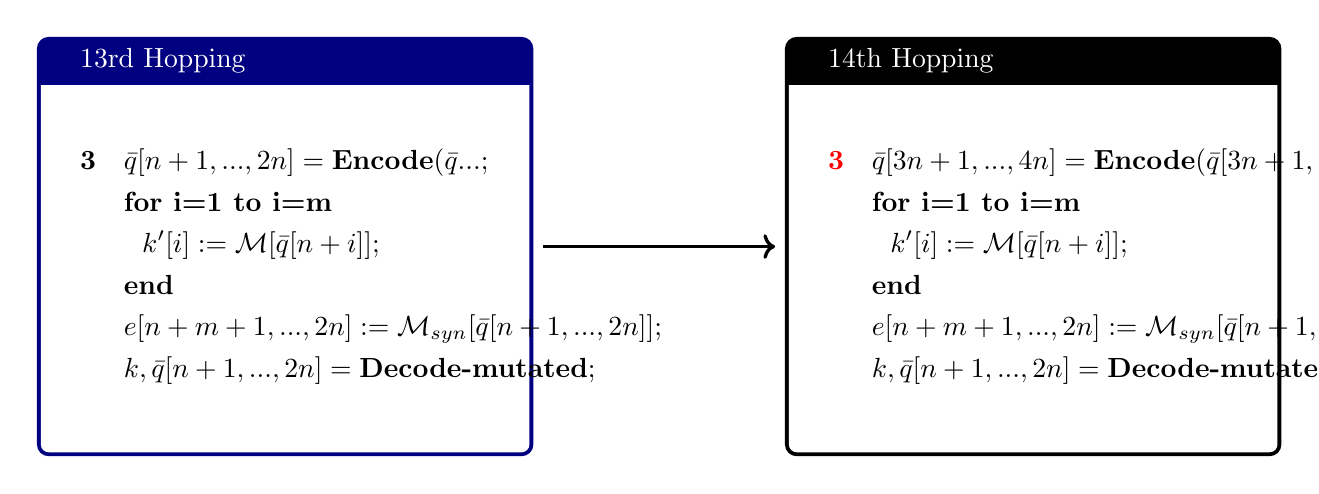
\begin{tikzpicture}[remember picture]

% Left box
\node[anchor=north west] (leftbox) at (0,0) {
\begin{minipage}[t]{0.52\textwidth}
\begin{tcolorbox}[colframe=blue!50!black, colback=white, title=13rd Hopping, width=\textwidth]
\begin{align*}
    \textbf{{3}} \quad &\bar{q}[n+1,...,2n]=\textbf{Encode}(\bar{q}...;\\
    & \textbf{for i=1 to i=m}\\
    &~~ k'[i]:= \mathcal{M} [\bar{q}[n+i]];\\
    &\textbf{end}\\
    & e[n+m+1,...,2n]:=\mathcal{M}_{syn} [\bar{q}[n+1,...,2n]];\\
    & k,\bar{q}[n+1,...,2n]=\textbf{Decode-mutated};\\
\end{align*}
\end{tcolorbox}
\end{minipage}
};

% Right box
\node[anchor=north west] (rightbox) at (9.5,0) {
\begin{minipage}[t]{0.52\textwidth}
\begin{tcolorbox}[colframe=black!50!black, colback=white, title=14th Hopping, width=\textwidth]
\begin{align*}
    \textbf{\textcolor{red}{3}} \quad 
    &\bar{q}[3n+1,...,4n]=\textbf{Encode}(\bar{q}[3n+1,...,3n+m])\\
    & \textbf{for i=1 to i=m}\\
    &~~ k'[i]:= \mathcal{M} [\bar{q}[n+i]];\\
    &\textbf{end}\\
    & e[n+m+1,...,2n]:=\mathcal{M}_{syn} [\bar{q}[n+1,...,2n]];\\
    & k,\bar{q}[n+1,...,2n]=\textbf{Decode-mutated};\\
\end{align*}
\end{tcolorbox}
\end{minipage}
};

% Draw arrow between boxes
\draw[->, very thick] (leftbox.east) -- node[above]{} (rightbox.west);

\end{tikzpicture}


\textbf{13th Hopping and 14th Hopping:}
$$
P:\textbf{3}; \sim P':\textbf{3};~~~~~~~\{\equiv\}\Rightarrow \{\equiv\}~~~~~~~~(SC: (P_C^{A}\!\otimes P_C^{B})|\Phi^+\rangle^{\otimes n}=P_C^{A}|\Phi^+\rangle^{\otimes n}=P_C^{B}|\Phi^+\rangle^{\otimes n})
$$

\newpage


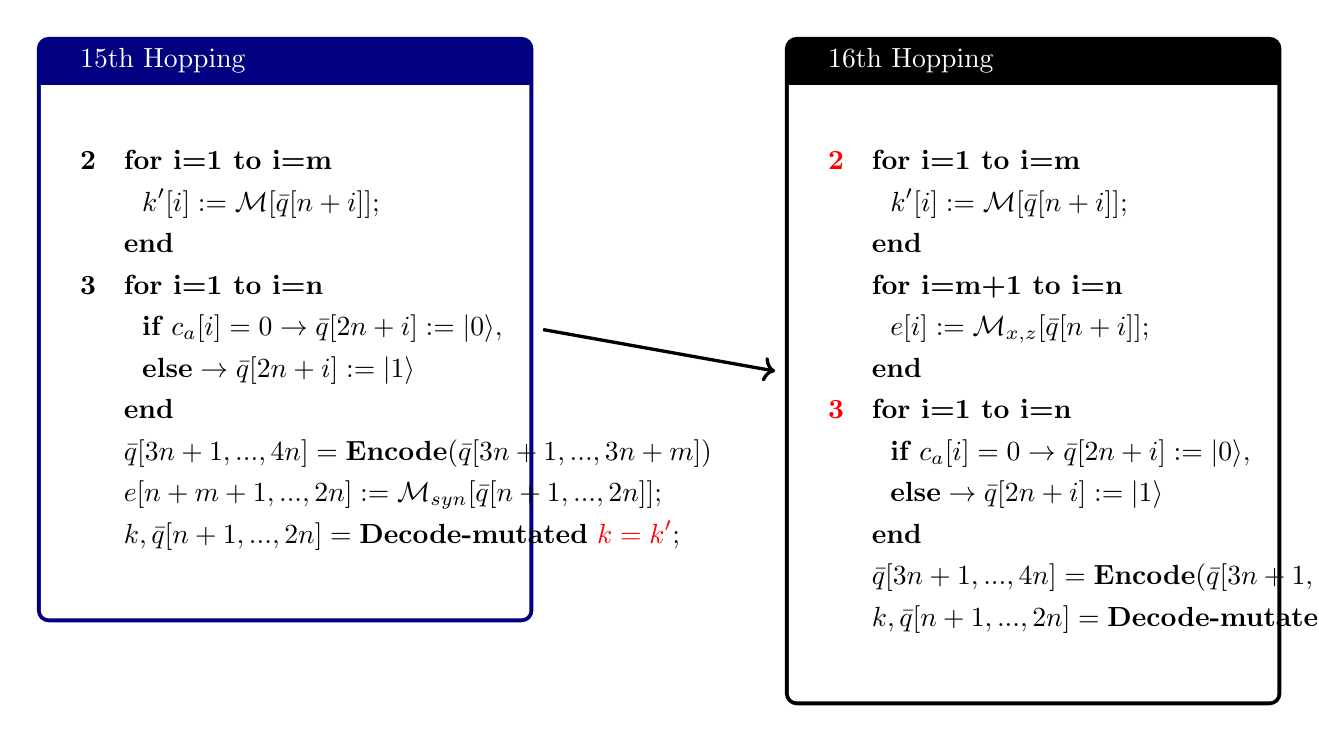
\begin{tikzpicture}[remember picture]

% Left box
\node[anchor=north west] (leftbox) at (0,0) {
\begin{minipage}[t]{0.52\textwidth}
\begin{tcolorbox}[colframe=blue!50!black, colback=white, title=15th Hopping, width=\textwidth]
\begin{align*}
    \textbf{{2}} \quad 
    & \textbf{for i=1 to i=m}\\
    &~~ k'[i]:= \mathcal{M} [\bar{q}[n+i]];\\
    &\textbf{end}\\
    \textbf{{3}} \quad 
    &\textbf{for i=1 to i=n}\\
    &~~ \textbf{if }  c_a[i] = 0 \rightarrow \bar{q}[2n+i] := |0\rangle,\\ &~~\textbf{else}   \rightarrow \bar{q}[2n+i] := |1\rangle\\
    &\textbf{end}\ \\
    &\bar{q}[3n+1,...,4n]=\textbf{Encode}(\bar{q}[3n+1,...,3n+m])\\ 
    & e[n+m+1,...,2n]:=\mathcal{M}_{syn} [\bar{q}[n+1,...,2n]];\\
    & k,\bar{q}[n+1,...,2n]=\textbf{Decode-mutated} ~\textcolor{red}{k=k'};\\
\end{align*}
\end{tcolorbox}
\end{minipage}
};

% Right box
\node[anchor=north west] (rightbox) at (9.5,0) {
\begin{minipage}[t]{0.52\textwidth}
\begin{tcolorbox}[colframe=black!50!black, colback=white, title=16th Hopping, width=\textwidth]
\begin{align*}
    \textbf{\textcolor{red}{2}} \quad 
    & \textbf{for i=1 to i=m}\\
    &~~ k'[i]:= \mathcal{M} [\bar{q}[n+i]];\\
    &\textbf{end}\\
    &\textbf{for i=m+1 to i=n}\\
    &~~ e[i]:=\mathcal{M}_{x,z} [\bar{q}[n+i]];\\
    &\textbf{end}\\
    \textbf{\textcolor{red}{3}} \quad 
    &\textbf{for i=1 to i=n}\\
    &~~ \textbf{if }  c_a[i] = 0 \rightarrow \bar{q}[2n+i] := |0\rangle,\\ &~~\textbf{else}   \rightarrow \bar{q}[2n+i] := |1\rangle\\
    &\textbf{end}\ \\
    \quad 
    &\bar{q}[3n+1,...,4n]=\textbf{Encode}(\bar{q}[3n+1,...,3n+m])\\
    &k,\bar{q}[n+1,...,2n]=\textbf{Decode-mutated} ~\textcolor{red}{k=k'}\\
\end{align*}
\end{tcolorbox}
\end{minipage}
};

% Draw arrow between boxes
\draw[->, very thick] (leftbox.east) -- node[above]{} (rightbox.west);

\end{tikzpicture}


\textbf{15th Hopping and 16th Hopping:}
$$
P; \sim P'; ~~~~~~\{\equiv\}\Rightarrow \{\equiv\}~~~~~~(SC: (\mathbb I\!\otimes P_C),\ket{\Phi^{+}}^{\otimes n}
  \;=\;
(U_{\text{enc}}^{\dagger}\!\otimes U_{\text{enc}}^{\dagger})
\!\Bigl[
    \mathbb I_L\!\otimes\!\mathbb I_L
    \otimes
    \ket{0}\!\bra{0}^{\otimes 2(n-k)}
 \Bigr]
(U_{\text{enc}}\!\otimes U_{\text{enc}})
\ket{\Phi^{+}}^{\otimes n})
$$
where $P$ is:
\begin{align*}
    \quad &\bar{q}[3n+1,...,4n]=\textbf{Encode}(\bar{q}[3n+1,...,3n+m])\\
    & e[i]:= \mathcal{M}_{synrome} [\bar{q}[i]];\\
\end{align*}

and $P'$ is:
\begin{align*}
    \quad 
    & \textbf{for i=m+1 to i=n}\\
    &~~ e[n+i]:= \mathcal{M}_{x,z} [\bar{q}[n+i]];\\
    &\textbf{end}\\
    \quad 
    &\bar{q}[3n+1,...,4n]=\textbf{Encode}(\bar{q}[3n+1,...,3n+m])\\ 
\end{align*}

$$
P'_1; \sim P'_2; ~~~~~~~\{\equiv\}\Rightarrow \{\equiv\}~~~~~~~(SWAP)
$$
where $P'_1$ is:
\begin{align*}
    \quad &\textbf{for i=1 to i=n}\\
    &~~ \textbf{if }  c_a[i] = 0 \rightarrow \bar{q}[2n+i] := |0\rangle,\\ &~~\textbf{else}   \rightarrow \bar{q}[2n+i] := |1\rangle\\
    &\textbf{end}\ \\
    & \textbf{for i=m+1 to i=n}\\
    &~~ e[n+i]:= \mathcal{M}_{x,z} [\bar{q}[n+i]];\\
    &\textbf{end}\\
\end{align*}

and $P'_2$ is:
\begin{align*}
    \quad 
    & \textbf{for~i=m+1~to~i=n}\\
    &~~ e[i]:= \mathcal{M}_{x,z} [\bar{q}[3n+i]];\\
    &\textbf{end}\\
    \quad 
    &\textbf{for i=1 to i=n}\\
    &~~ \textbf{if }  c_a[i] = 0 \rightarrow \bar{q}[i] := |0\rangle,\\ &~~\textbf{else}   \rightarrow \bar{q}[i] := |1\rangle\\
    &\textbf{end}\ \\
\end{align*}

\newpage

\subsection{Resource-Certified Relational Hopping for Lo--Chau, CSS, and BB84}
\label{subsec:resource-certified-hopping-final}

This subsection gives the command-level proof certificate for the two reduction
chains
\[
  \textsf{Modified Lo--Chau Protocol}
  \leadsto
  \textsf{CSS Code Protocol}
  \qquad\text{and}\qquad
  \textsf{CSS Code Protocol}
  \leadsto
  \textsf{BB84 Protocol}.
\]
The optional BBM92 branch is not used in this proof.  We write the population
slack as \(\lambda\).  All checkpoint names below follow the technical-report
hopping notation: we refer to the \(i\)-th displayed transformation as
\emph{Hopping \(i\)}, not as a figure node \(G_i\).

The central convention is the following.  No relational rule application is
accepted merely because its local side condition has been asserted.  Instead,
every local resource premise used by a relational rule must be derived from the
beginning of the current Hopping by the auxiliary resource judgment.  Thus a
relational rule is discharged only after running the appropriate resource prefix
and extracting its endpoint \(\Omega\)-context.

\paragraph{Notation.}
We use the following shorthand:
\[
\providecommand{\res}{\mathsf{res}}
\providecommand{\rel}{\mathsf{rel}}
\providecommand{\Live}{\operatorname{Live}}
\providecommand{\Fresh}{\operatorname{Fresh}}
\providecommand{\AllocOK}{\operatorname{AllocOK}}
\providecommand{\Own}{\operatorname{Own}}
\providecommand{\Req}{\operatorname{Req}_{\mathsf{res}}}
\providecommand{\acc}{\operatorname{acc}}
\providecommand{\upd}{\operatorname{upd}}
\providecommand{\Obs}{\operatorname{Obs}}
\providecommand{\susp}{\mathsf{susp}}
\providecommand{\asteq}{\mathrel{\ast\!\!=}}
\providecommand{\HopLC}[1]{\mathsf{LC}^{[#1]}}
\providecommand{\HopBB}[1]{\mathsf{BB}^{[#1]}}
\providecommand{\Out}{\mathsf{Out}}
\providecommand{\term}{\mathsf{term}}
\]
When these macros already exist in the manuscript, this paragraph should be
deleted.

\subsubsection{The Resource System Used by the Hop Certificates}
\label{subsubsec:resource-system-hop-certificates-final}

\paragraph{Resource contexts.}
A resource context has the form
\[
\Omega =
\bigl(
  Q_{\mathsf{live}},
  C_{\mathsf{live}},
  D_{\mathsf{desc}},
  Q_{\mathsf{susp}},
  C_{\mathsf{susp}},
  \mathsf{Own},
  L,
  \Obs
\bigr).
\]
Here \(Q_{\mathsf{live}}\) and \(C_{\mathsf{live}}\) are the live quantum and
classical roots.  The descriptor map \(D_{\mathsf{desc}}\) resolves displayed
views, such as \(\bar q[i]\), \(\bar q[I]\), \(x[I]\), and \(b[I]\), to owned
physical roots or slices.  The sets \(Q_{\mathsf{susp}}\) and
\(C_{\mathsf{susp}}\) contain suspended descriptors that may remain in the
semantic store but cannot discharge a later \(\Live\), \(\#\), or \(\Own\)
premise.  The component \(\mathsf{Own}\) records singleton ownership tokens used
by append, partition, and select.  The transcript root \(L\) is append-only and
persistent; publication copies a classical value into a fresh transcript cell and
does not consume the source root.

We write
\[
  \Omega \models \Live(v)
\]
when the descriptor \(v\) resolves to a live root or live slice.  We write
\[
  \Omega \models v \# w
\]
when \(v\) and \(w\) resolve to disjoint live physical supports.  We write
\[
  \Omega \models \Fresh(v)
\]
when \(v\) has not been allocated in the current branch.  We write
\[
  \Omega \models \AllocOK(v)
\]
when \(v\) is available for allocation in the current live interface: either it
is fresh, or it is a suspended descriptor that can be reintroduced only through
an explicit allocation, reset, or superoperator-output rule.  Thus the proof may
reuse a displayed name such as \(\bar q[1{:}m]\) only after the earlier live root
occupying that view has been suspended.

Two distinct live roots never denote the same physical address.  Two surface
names may denote the same physical address only when one descriptor is suspended
and the other is the unique live owned alias.

For compactness, write
\[
  \Omega\oplus v
\]
for the context obtained by removing \(v\) from the suspended or allocable
component, if present, and inserting \(v\) as a live root.  Likewise,
\[
  \Omega+\susp(v)
\]
means that the descriptor \(v\) is retained only as suspended metadata and cannot
be used to discharge later liveness or ownership premises.

\paragraph{Primitive and derived resource rules.}
The resource judgment is written
\[
  \Omega\vdash_{\mathsf{res}} P:\Omega' .
\]

\[
\frac{}{\Omega\vdash_{\mathsf{res}}\mathbf{skip}:\Omega}
\tag{\textsc{Res-Skip}}
\]

\[
\frac{
  \Omega\vdash_{\mathsf{res}}P:\Omega'
  \qquad
  \Omega'\vdash_{\mathsf{res}}Q:\Omega''
}{
  \Omega\vdash_{\mathsf{res}}P;Q:\Omega''
}
\tag{\textsc{Res-Seq}}
\]

\[
\frac{
  \Omega\models\AllocOK(c)
}{
  \Omega\vdash_{\mathsf{res}}
  c:=_\$\mathsf{rand}(d)
  :
  \Omega\oplus c{:}\mathsf{classical}(d)
}
\tag{\textsc{Res-Rand}}
\]

\[
\frac{
  \Omega\models\Live(e)
  \qquad
  \Omega\models\Live(L)
}{
  \Omega\vdash_{\mathsf{res}}
  \mathbf{publish}(e)
  :
  \Omega[L\mapsto L\mathbin{\|}e]
}
\tag{\textsc{Res-Publish}}
\]
Publication is value-copy into a transcript cell.  It does not create an alias
for \(e\), does not consume \(e\), and does not introduce a new linear root for
the copied transcript cell.

\[
\frac{
  \Omega\models\AllocOK(q)
}{
  \Omega\vdash_{\mathsf{res}}
  q:=\ket 0^{\otimes r}
  :
  \Omega\oplus q{:}\mathsf{quantum}(r)
}
\tag{\textsc{Res-QInit}}
\]

For resetting a live target, we use the derived rule
\[
\frac{
  \Omega\models\Live(q)
}{
  \Omega\vdash_{\mathsf{res}}
  q:=\ket0
  :
  \Omega
}
\tag{\textsc{Res-QReset}}
\]
and its \(r\)-qubit extension.  This rule is used when a displayed branch
initialization is a reset of the same live target, not a fresh allocation.

\[
\frac{
  \Omega\models\Live(q_1),\ldots,\Omega\models\Live(q_r)
  \qquad
  \Omega\models q_i\#q_j\quad(i\neq j)
}{
  \Omega\vdash_{\mathsf{res}}
  (q_1,\ldots,q_r)\asteq U
  :
  \Omega
}
\tag{\textsc{Res-Unitary}}
\]

\[
\frac{
  \Omega\models\Live(q_1)
  \qquad
  \Omega\models\Live(q_2)
  \qquad
  \Omega\models q_1\#q_2
}{
  \Omega\vdash_{\mathsf{res}}
  (q_1,q_2)\asteq\mathrm{CNOT}
  :
  \Omega
}
\tag{\textsc{Res-CNOT}}
\]

\[
\frac{
  \Omega\models\Live(q)
  \qquad
  \Omega\models\AllocOK(c)
}{
  \Omega\vdash_{\mathsf{res}}
  c:=\mathcal M[q]
  :
  \Omega\oplus c{:}\mathsf{classical}
}
\tag{\textsc{Res-Meas}}
\]

For a destructive measurement followed by removal of the measured view from the
proof interface, we use:
\[
\frac{
  \Omega\models\Live(q)
  \qquad
  \Omega\models\AllocOK(c)
}{
  \Omega\vdash_{\mathsf{res}}
  c:=\mathcal M[q];\mathbf{drop}(q)
  :
  \Omega-q+\susp(q)+c{:}\mathsf{classical}
}
\tag{\textsc{Res-MeasDrop}}
\]

\[
\frac{
  \Omega\models\Live(g)
  \qquad
  \Omega_g^0\vdash_{\mathsf{res}}P_0:\Omega_0'
  \qquad
  \Omega_g^1\vdash_{\mathsf{res}}P_1:\Omega_1'
  \qquad
  \Omega_0'\Join\Omega_1'\ \text{defined}
}{
  \Omega\vdash_{\mathsf{res}}
  \mathbf{if}\ g=0\rightarrow P_0\ \mathbf{else}\ P_1
  :
  \Omega_0'\Join\Omega_1'
}
\tag{\textsc{Res-If}}
\]

\[
\frac{
  \mathcal I(0)=\Omega_0
  \qquad
  \forall i<r,\ 
  \mathcal I(i)\vdash_{\mathsf{res}}P(i):\mathcal I(i+1)
}{
  \Omega_0\vdash_{\mathsf{res}}
  \mathbf{for}\ i=1\ \mathbf{to}\ r\ \mathbf{do}\ P(i)
  :
  \mathcal I(r)
}
\tag{\textsc{Res-For}}
\]

\[
\frac{
  \Omega\models\Live(v)
}{
  \Omega\vdash_{\mathsf{res}}
  \mathbf{drop}(v)
  :
  \Omega-v+\susp(v)
}
\tag{\textsc{Res-Drop}}
\]

\[
\frac{
  \Omega\models\Live(r)
  \qquad
  I_1,\ldots,I_k\ \text{partition the support of }r
}{
  \Omega\vdash_{\mathsf{res}}
  r\Rightarrow r[I_1]\uplus\cdots\uplus r[I_k]
  :
  \Omega-r+\{r[I_j]\}_{j=1}^k
}
\tag{\textsc{Res-Split}}
\]

\[
\frac{
  \Omega\models\Live(r)
}{
  \Omega\vdash_{\mathsf{res}}
  r\Rightarrow \biguplus_{i=1}^{|r|}r[i]
  :
  \Omega-r+\{r[i]\}_{i=1}^{|r|}
}
\tag{\textsc{Res-SplitSingleton}}
\]

\[
\frac{
  \Omega\models\Own(v)
  \qquad
  \Omega\models\Live(d)
  \qquad
  \Omega\models v\# d
}{
  \Omega\vdash_{\mathsf{res}}
  \mathbf{append}(d,v)
  :
  \Omega-v+(d\mathbin{\|}v)
}
\tag{\textsc{Res-Append}}
\]

\[
\frac{
  \Omega\models\Own(v_i)
  \qquad
  \Omega\models v_i\#v_j\quad(i\neq j)
}{
  \Omega\vdash_{\mathsf{res}}
  d:=\mathbf{concat}(v_1,\ldots,v_k)
  :
  \Omega-\{v_i\}_{i=1}^k+d
}
\tag{\textsc{Res-Concat}}
\]

\[
\frac{
  \Omega\models\Live(x,b,\bar q)
  \qquad
  \Omega\models\Live(f)
  \qquad
  f\ \text{is duplicate-free}
}{
  \Omega\vdash_{\mathsf{res}}
  (x',b',\bar q'):=\mathbf{select}_f(x,b,\bar q)
  :
  \Omega-x-b-\bar q+\susp(x,b,\bar q)+x'+b'+\bar q'
}
\tag{\textsc{Res-Select}}
\]
The old source roots are suspended after selection.  They may remain as semantic
descriptors, but they cannot discharge later \(\Live\), \(\#\), or \(\Own\)
premises.

The explicit guarded append loop is certified by the derived rule:
\[
\frac{
  \Omega\vdash_{\mathsf{res}}
  r\Rightarrow\biguplus_i r[i]:\Omega_1
  \qquad
  \forall i,\ 
  \Omega_i\vdash_{\mathsf{res}}
  \begin{cases}
    \mathbf{append}(d,r[i]) & \text{if the guard accepts }i,\\
    \mathbf{drop}(r[i]) & \text{otherwise}
  \end{cases}
  :
  \Omega_{i+1}
}{
  \Omega\vdash_{\mathsf{res}}
  d:=\mathbf{selectLoop}_{G}(r)
  :
  \Omega_{\mathsf{out}}
}
\tag{\textsc{Res-SelectLoop}}
\]
In this derived rule, every source singleton is either transferred exactly once
into an output descriptor or suspended/dropped.  No quantum state and no
classical value is copied.

\[
\frac{
  \Omega\models\Live(A)
  \qquad
  \Omega\models\AllocOK(a_Z,a_X)
  \qquad
  \Omega\models\AllocOK(s_Z,s_X)
}{
  \Omega\vdash_{\mathsf{res}}
  (s_Z,s_X):=\mathsf{CSSSyn}_{H_Z,H_X}(A;a_Z,a_X)
  :
  \Omega\oplus a_Z\oplus a_X\oplus s_Z\oplus s_X
}
\tag{\textsc{Res-CSSSyn}}
\]

\[
\frac{
  \Omega\models\Live(A)
  \qquad
  \Omega\models\AllocOK(A')
  \qquad
  \Omega\models\AllocOK(\mathsf{anc})
}{
  \Omega\vdash_{\mathsf{res}}
  A':=QEC(A;\mathsf{anc})
  :
  \Omega-A+\susp(A)+A'+\mathsf{anc}
}
\tag{\textsc{Res-QEC}}
\]

\[
\frac{
  \Omega\models\Live(\bar q_{\mathsf{in}})
  \qquad
  \Omega\models\Live(\bar q_{\mathsf{eve}})
  \qquad
  \Omega\models \bar q_{\mathsf{in}}\#\bar q_{\mathsf{eve}}
}{
  \Omega\vdash_{\mathsf{res}}
  (\bar q_{\mathsf{in}},\bar q_{\mathsf{eve}})
  \asteq U_{\mathsf{channel}}
  :
  \Omega
}
\tag{\textsc{Res-Channel}}
\]

\[
\frac{}{\Omega\vdash_{\mathsf{res}}\mathbf{abort}:\Omega_{\mathsf{abort}}}
\tag{\textsc{Res-Abort}}
\]

\paragraph{Hop certificates, endpoint alignment, and observation extraction.}
For every Hopping
\[
  H_i:\qquad P_i\leadsto P_{i+1},
\]
the certificate has three layers.

First, it contains resource traces for the displayed left and right programs:
\[
  \vdash_{\mathsf{res}}P_i:
  \Omega_i^L\longrightarrow\widehat\Omega_i^L,
  \qquad
  \vdash_{\mathsf{res}}P_{i+1}:
  \Omega_i^R\longrightarrow\widehat\Omega_i^R.
\]
Second, it contains an endpoint resource-alignment certificate
\[
  \widehat\Omega_i^L\simeq_{\theta_i}\widehat\Omega_i^R,
\tag{Endpoint-Align}
\]
where \(\theta_i\) is a harmless renaming of presentation descriptors and where
the retained observation views are identified exactly.  The relational
postcondition of the Hopping is extracted only after this endpoint alignment has
been applied.

Third, after the endpoint alignment, the retained terminal observation extractor
\[
  \mathsf{obs}_i:\widehat\Omega_i\to(K_A,K_B,L,\mathsf E)
\tag{Obs-Extractor}
\]
is applied.  The Hopping certificate is accepted only when the relational
postcondition implies equality of the extracted retained views.  Thus every
Hopping has the closed shape
\[
  \text{resource trace}
  \quad+\quad
  \text{local relational judgment}
  \quad+\quad
  \text{terminal observation extraction}.
\]

The retained transcript convention is fixed as follows.  In the CSS phase-frame
elimination Hopping, \(L\) means \(L^{\setminus z}\), the authenticated
transcript after erasing the displayed \(z\)-publication cells.  In all other
exact Hoppings, \(L\) denotes the retained public transcript specified by the
technical-report protocol checkpoint.

\paragraph{Resource-prefix admissibility of relational rules.}
For a Hopping
\[
  H:\quad P\leadsto P',
\]
and for a relational rule \(R\) applied at an internal node \(\nu\), let
\[
  P_{\preceq\nu}=S_1;\cdots;S_t
\]
be the prefix of the displayed side of the Hopping from the first statement of
that Hopping to the rule application point.  The relational rule application is
resource-admissible only if there exists a prefix derivation
\[
  \mathsf{Run}_{\mathsf{res}}(H,\nu):
  \qquad
  \Omega_0^H
  \vdash_{\mathsf{res}}
  S_1;\cdots;S_t
  :
  \Omega_\nu^H
\]
such that
\[
  \Omega_\nu^H\models \Req(R,\nu).
\]
Equivalently, the admissible relational rule form is:
\[
\frac{
  \Omega_0^H\vdash_{\mathsf{res}}P_{\preceq\nu}:\Omega_\nu^H
  \qquad
  \Omega_\nu^H\models\Req(R,\nu)
  \qquad
  \Xi\vdash_R P\sim P':\Phi\Rightarrow\Psi
}{
  \Xi;\Omega_0^H
  \vdash
  P\sim P':\Phi\Rightarrow\Psi
}.
\tag{\textsc{ResRel-Admiss}}
\]
Thus the proof never uses a free-standing assertion such as
``\(q[i]\) is live''.  Every such assertion must be the endpoint of a prefix
resource run.

For the rules used below, the relevant resource requirements are:
\[
\Req(\textsc{Swap}(P_0,P_1),\nu)
\equiv
\Live(\acc(P_0)\cup\acc(P_1))
\land
\acc(P_0)\#\acc(P_1)
\land
\upd(P_0)\#\upd(P_1),
\]
together with typability of both execution orders from the same input resource:
\[
  \Omega_\nu\vdash_{\mathsf{res}}P_0;P_1:\Omega^\star
  \qquad
  \Omega_\nu\vdash_{\mathsf{res}}P_1;P_0:\Omega^\star .
\]

\[
\Req(\textsc{CNOT}(q_1,q_2),\nu)
\equiv
\Live(q_1)\land\Live(q_2)\land q_1\#q_2 .
\]

For a \(\textsc{Uniform}\) node, the resource certificate contains both a
pre-node and a post-node context:
\[
  \Omega_0^H\vdash_{\mathsf{res}}P_{\prec\nu}:\Omega_\nu^{\mathsf{pre}},
  \qquad
  \Omega_\nu^{\mathsf{pre}}
  \models
  \Live(q)\land \AllocOK(c)\land q\notin\Obs_{\mathsf{retained}},
\tag{Uniform-Pre}
\]
and
\[
  \Omega_\nu^{\mathsf{pre}}
  \vdash_{\mathsf{res}}
  c:=\mathcal M[q];\mathbf{drop}(q)
  :
  \Omega_\nu^{\mathsf{post}},
  \qquad
  \Omega_\nu^{\mathsf{post}}\models q\in Q_{\mathsf{susp}}.
\tag{Uniform-Post}
\]
The relational \(\textsc{Uniform}\) rule is applied at
\(\Omega_\nu^{\mathsf{pre}}\), while later rule applications use
\(\Omega_\nu^{\mathsf{post}}\).

\[
\Req(\textsc{If-Stru}(g),\nu)
\equiv
\Live(g)
\land
\upd(P_{\mathsf{then}})\#\acc(g)
\land
\upd(P_{\mathsf{else}})\#\acc(g),
\]
with both branches resource-typable and joinable.

\[
\Req(\textsc{IID},\nu)
\equiv
\Live(x,b,f)
\land |x|=|b|=N
\land
f\in\mathsf{Shuffle}(r,N)
\land
\mathsf{IidFit}_N(x,f)
\land
\mathsf{IidFit}_N(b,f).
\]

\[
\Req(\textsc{Sift},\nu)
\equiv
\text{both resource traces end with the same retained classical roots}
\]
after comparing the quantum-first trace and the measure-first trace.

\[
\Req(\textsc{CSS},\nu)
\equiv
\Live(A)\land\AllocOK(a_Z,a_X,s_Z,s_X)
\land
\operatorname{AncFresh}_{\Omega}(A;a_Z,a_X).
\]

\[
\Req(\textsc{PublicExt}(e),\nu)
\equiv
\AllocOK(e)\land\Live(L),
\]
and the same public extension must be applied on both sides of the relational
comparison.

\paragraph{Quantum frames.}
The swap steps below use only resolved access-disjointness from the current
\(\Omega\)-context.  They do not assume product structure.  A
\(\textsc{Quantum-Frame}\) instance is used only when a quantum assertion is
carried unchanged around a local derivation.  In that case, the side condition
\[
  \Xi\models \operatorname{Sep}(U:F)
\]
is discharged at the rule instance.  The resource judgment proves liveness,
ownership, freshness, and physical disjointness; it is not used as a surrogate
for separability.

\subsubsection{Modified Lo--Chau Protocol to CSS Code Protocol}
\label{subsubsec:lc-css-resource-certified-ledger-final}

Write the four \(n\)-qubit slices of the Lo--Chau \(4n\)-qubit block as
\[
  A_c=\bar q[1{:}n],
  \qquad
  A_k=\bar q[n+1{:}2n],
  \qquad
  B_c=\bar q[2n+1{:}3n],
  \qquad
  B_k=\bar q[3n+1{:}4n].
\]
The \(c\)-subscript denotes check positions and the \(k\)-subscript denotes key
positions.

Let
\[
  \HopLC{0},\HopLC{1},\ldots,\HopLC{12}
\]
denote the technical-report Lo--Chau-to-CSS checkpoints, where
\(\HopLC{0}\) is the Modified Lo--Chau Protocol before the first displayed
Hopping, \(\HopLC{i}\) is the checkpoint after Hopping \(i\), and
\(\HopLC{12}\) is the CSS Code Protocol.  These indices are proof-ledger
indices, not additional protocol nodes.

The initial resource context is
\[
\Omega^{\mathrm{LC}}_0
=
\{
  L:\mathsf{live}_C,\ 
  \bar q[1{:}4n]:\mathsf{allocable}_Q,\ 
  c_a,c_b,k,f_{\mathbf c},b:\mathsf{allocable}_C,\ 
  \bar q_{\mathsf{eve}}:\mathsf{live}_Q
\}.
\]

\paragraph{Common Lo--Chau EPR prefix.}
The EPR-preparation prefix used by the first Lo--Chau Hoppings is
\[
\mathsf{EPRPrep}_{\mathrm{LC}}
\equiv
\bar q[1{:}4n]:=\ket0^{\otimes 4n};
\quad
\bar q[1{:}4n]\Rightarrow A_c\uplus A_k\uplus B_c\uplus B_k;
\]
\[
\mathbf{for}\ i=1\ \mathbf{to}\ n\ \mathbf{do}\ 
  A_c[i]\asteq H;
  (A_c[i],B_c[i])\asteq\mathrm{CNOT};
  A_k[i]\asteq H;
  (A_k[i],B_k[i])\asteq\mathrm{CNOT}
\ \mathbf{end}.
\]
The resource derivation is:
\[
\begin{aligned}
\Omega^{\mathrm{LC}}_0
&\xrightarrow{\textsc{Res-QInit}(\bar q[1{:}4n])}
\Omega^{\mathrm{LC}}_1
\\
&\xrightarrow{\textsc{Res-Split}(\bar q[1{:}4n])}
\Omega^{\mathrm{LC}}_2
=
\Omega^{\mathrm{LC}}_1-\bar q[1{:}4n]+A_c+A_k+B_c+B_k
\\
&\xrightarrow{\textsc{Res-For}+\textsc{Res-Unitary}(H)}
\Omega^{\mathrm{LC}}_3
\\
&\xrightarrow{\textsc{Res-For}+\textsc{Res-CNOT}}
\Omega^{\mathrm{LC}}_4 .
\end{aligned}
\tag{LC-EPR-Prefix}
\]
At the endpoint,
\[
\Omega^{\mathrm{LC}}_4
\models
\Live(A_c,A_k,B_c,B_k)
\land
A_c\#A_k\#B_c\#B_k.
\tag{LC-EPR}\label{LC-EPR}
\]

\paragraph{Hopping 1: moving Alice's check measurement.}
The moved block is
\[
M_A^c
\equiv
\mathbf{for}\ i=1\ \mathbf{to}\ n\ \mathbf{do}\ 
c_a[i]:=\mathcal M_{\mathrm{com}}[A_c[i]];
\mathbf{drop}(A_c[i])
\ \mathbf{end}.
\]
The relational rule node is the swap of \(M_A^c\) with the crossed suffix
\(C_{\mathrm{rest}}\).  The required prefix resource certificate is:
\[
\Omega^{\mathrm{LC}}_0
\vdash_{\mathsf{res}}
\mathsf{EPRPrep}_{\mathrm{LC}}
:
\Omega^{\mathrm{LC}}_4 .
\tag{LC-H1-Prefix}\label{LC-H1-Prefix}
\]
By \eqref{LC-EPR},
\[
\Omega^{\mathrm{LC}}_4
\models
\Live(A_c)
\land
\AllocOK(c_a[1{:}n])
\land
A_c\#(A_k\uplus B_c\uplus B_k).
\]
The crossed suffix accesses
\[
\acc(C_{\mathrm{rest}})
\subseteq
\{f_{\mathbf c},b,L,\bar q_{\mathsf{eve}},A_k,B_c,B_k,c_b,k[m+1{:}2m]\},
\]
and does not access \(A_c\) or \(c_a[1{:}n]\).  Therefore
\[
\Omega^{\mathrm{LC}}_4
\models
\{A_c,c_a[1{:}n]\}\#\acc(C_{\mathrm{rest}}).
\tag{LC-H1-SwapReq}
\]
The moved measurement block is itself resource-checked:
\[
\begin{aligned}
\Omega^{\mathrm{LC}}_4
&\xrightarrow{
  \textsc{Res-For}
  \left(
    \forall i\le n,\ 
    \textsc{Res-MeasDrop}(A_c[i],c_a[i])
  \right)}
\Omega^{\mathrm{LC}}_5
\\
&=
\Omega^{\mathrm{LC}}_4
-A_c+\susp(A_c)+c_a[1{:}n].
\end{aligned}
\tag{LC-H1-MeasRun}
\]
Both orders are typable from \(\Omega^{\mathrm{LC}}_4\):
\[
\Omega^{\mathrm{LC}}_4
\vdash_{\mathsf{res}}
M_A^c;C_{\mathrm{rest}}:\widehat\Omega^{\mathrm{LC}}_1,
\qquad
\Omega^{\mathrm{LC}}_4
\vdash_{\mathsf{res}}
C_{\mathrm{rest}};M_A^c:\widehat\Omega^{\mathrm{LC}}_1.
\]
Hence
\[
\Xi^{\mathrm{LC}}_1
\vdash
\HopLC{0}\sim\HopLC{1}:
\equiv_{\mathcal V^{\mathrm{LC}}_0}
\Longrightarrow
\equiv_{\mathcal V^{\mathrm{LC}}_1}
\tag{LC-H1-Rel}
\]
by \(\textsc{Swap}\).  This Hopping has loss \(0\).  The endpoint
alignment \(\widehat\Omega_1^L\simeq_{\theta_1}\widehat\Omega_1^R\) identifies
the same retained views after the presentation move.

\paragraph{Hopping 2: CNOT-plus-measure to conditional \(X\).}
For each \(1\le i\le n\), the left fragment is
\[
L_i
\equiv
(A_c[i],B_c[i])\asteq\mathrm{CNOT};
\ c_a[i]:=\mathcal M_{\mathrm{com}}[A_c[i]];
\ \mathbf{drop}(A_c[i]).
\]
The right fragment is
\[
R_i
\equiv
c_a[i]:=\mathcal M_{\mathrm{com}}[A_c[i]];
\ \mathbf{drop}(A_c[i]);
\ \mathbf{if}\ c_a[i]=0\rightarrow\mathbf{skip}
\ \mathbf{else}\rightarrow B_c[i]\asteq X .
\]
The prefix to the \(i\)-th relational CNOT node is
\[
\Omega^{\mathrm{LC}}_0
\vdash_{\mathsf{res}}
\mathsf{EPRPrep}_{\mathrm{LC}};
L_1;\cdots;L_{i-1}
:
\Omega^{\mathrm{LC}}_{4,i}.
\tag{LC-H2-Prefix-i}\label{LC-H2-Prefix-i}
\]
The loop invariant gives
\[
\Omega^{\mathrm{LC}}_{4,i}
\models
\Live(A_c[i],B_c[i])
\land
A_c[i]\#B_c[i]
\land
\AllocOK(c_a[i])
\land
\Live(A_k,B_k).
\tag{LC-H2-CNOTReq-i}\label{LC-H2-CNOTReq-i}
\]
The left resource trace is
\[
\Omega^{\mathrm{LC}}_{4,i}
\xrightarrow{\textsc{Res-CNOT}(A_c[i],B_c[i])}
\Omega^{\mathrm{LC}}_{4,i,1}
\xrightarrow{\textsc{Res-MeasDrop}(A_c[i],c_a[i])}
\Omega^{\mathrm{LC}}_{4,i,2}.
\tag{LC-H2-LeftRun-i}\label{LC-H2-LeftRun-i}
\]
The right resource trace is
\[
\Omega^{\mathrm{LC}}_{4,i}
\xrightarrow{\textsc{Res-MeasDrop}(A_c[i],c_a[i])}
\widetilde\Omega^{\mathrm{LC}}_{4,i,1}
\xrightarrow{\textsc{Res-If}(c_a[i])+\textsc{Res-Unitary}(B_c[i])}
\widetilde\Omega^{\mathrm{LC}}_{4,i,2}.
\tag{LC-H2-RightRun-i}\label{LC-H2-RightRun-i}
\]
Both traces leave \(B_c[i]\) live and suspend \(A_c[i]\).  Therefore
\[
\frac{
  \eqref{LC-H2-Prefix-i}
  \qquad
  \eqref{LC-H2-CNOTReq-i}
  \qquad
  \eqref{LC-H2-LeftRun-i}
  \qquad
  \eqref{LC-H2-RightRun-i}
}{
  \Xi^{\mathrm{LC}}_{2,i}
  \vdash
  L_i\sim R_i:
  \Phi_{2,i}\Longrightarrow\Psi_{2,i}
}
\tag{LC-H2-PointwiseRel-i}
\]
by the pointwise \(\textsc{CNOT}\), \(\textsc{Meas}\), and
\(\textsc{If}\) rules.  Iterating with \(\textsc{SC+}\), \(\textsc{Seq}\),
and \(\textsc{Res-For}\) gives
\[
\Xi^{\mathrm{LC}}_2
\vdash
\HopLC{1}\sim\HopLC{2}:
\equiv_{\mathcal V^{\mathrm{LC}}_1}
\Longrightarrow
\equiv_{\mathcal V^{\mathrm{LC}}_2}.
\tag{LC-H2-Rel}
\]
This Hopping has loss \(0\).

\paragraph{Hopping 3: replacing Alice check readout by randomness.}
The uniformity replacement is
\[
c_a[1{:}n]:=\mathcal M_{\mathrm{com}}[A_c]
\quad\leadsto\quad
c_a:=_\$\mathbf{rand}(n).
\]
This Hopping uses the pre-node/post-node form of
\(\textsc{Uniform}\).  The pre-node prefix is
\[
\Omega^{\mathrm{LC}}_0
\vdash_{\mathsf{res}}
\mathsf{EPRPrep}_{\mathrm{LC}};
\mathbf{for}_{i=1}^n
\bigl((A_c[i],B_c[i])\asteq\mathrm{CNOT}\bigr)
:
\Omega^{\mathrm{LC},\mathsf{pre}}_{6}.
\tag{LC-H3-UniformPreRun}\label{LC-H3-UniformPreRun}
\]
At the uniformity node,
\[
\Omega^{\mathrm{LC},\mathsf{pre}}_{6}
\models
\Live(A_c,B_c,A_k,B_k)
\land
\AllocOK(c_a[1{:}n])
\land
A_c\notin\Obs_{\mathsf{retained}}.
\tag{LC-H3-UniformPreReq}
\]
The post-node resource trace is
\[
\Omega^{\mathrm{LC},\mathsf{pre}}_{6}
\vdash_{\mathsf{res}}
\mathbf{for}_{i=1}^n
\bigl(
  c_a[i]:=\mathcal M_{\mathrm{com}}[A_c[i]];
  \mathbf{drop}(A_c[i])
\bigr)
:
\Omega^{\mathrm{LC},\mathsf{post}}_{6},
\tag{LC-H3-UniformPostRun}\label{LC-H3-UniformPostRun}
\]
with
\[
\Omega^{\mathrm{LC},\mathsf{post}}_{6}
\models
\Live(c_a[1{:}n])
\land
A_c\in Q_{\mathsf{susp}}
\land
\Live(B_c,A_k,B_k)
\land
c_a[1{:}n]\#\acc(\text{later quantum commands}).
\tag{LC-H3-UniformPostReq}
\]
The semantic premise is that, after exposing the CNOT correlation, the measured
Alice check register has computational-basis uniform readout:
\[
\Xi^{\mathrm{LC}}_3
\models
A_c\ \text{has uniform computational-basis readout}
\land
A_c\notin\Obs_{\mathsf{retained}}.
\tag{LC-H3-UniformSemantic}
\]
The relational rule is
\[
\Xi^{\mathrm{LC}}_3
\vdash
\HopLC{2}\sim\HopLC{3}:
\equiv_{\mathcal V^{\mathrm{LC}}_2}
\Longrightarrow
\equiv_{\mathcal V^{\mathrm{LC}}_3}
\tag{LC-H3-Rel}
\]
by \(\textsc{Uniform}\), \(\textsc{If}\), and \(\textsc{Conseq}\).  The
post-node fact \(A_c\in Q_{\mathsf{susp}}\) is essential for later reuse of the
displayed addresses \(\bar q[1{:}m]\).

\paragraph{Hopping 4: isolating initialization of \(B_c\).}
The Hopping isolates the check-preparation target \(B_c\) from the key EPR
block.  The relevant prefix is:
\[
\Omega^{\mathrm{LC}}_0
\vdash_{\mathsf{res}}
A_k:=\ket0^{\otimes n};
B_k:=\ket0^{\otimes n};
\mathbf{for}_{i=1}^n
\bigl(
  A_k[i]\asteq H;
  (A_k[i],B_k[i])\asteq\mathrm{CNOT}
\bigr)
:
\Omega^{\mathrm{LC}}_7.
\tag{LC-H4-Prefix}\label{LC-H4-Prefix}
\]
At the initialization node for \(B_c\),
\[
\Omega^{\mathrm{LC}}_7
\models
\AllocOK(B_c)
\land
B_c\#A_k
\land
B_c\#B_k.
\tag{LC-H4-SwapReq}
\]
The initialization is resource-checked:
\[
\Omega^{\mathrm{LC}}_7
\xrightarrow{\textsc{Res-QInit}(B_c)}
\Omega^{\mathrm{LC}}_8.
\tag{LC-H4-QInit}
\]
Both execution orders are typable because the crossed commands access only
\(A_k,B_k\) and classical roots disjoint from \(B_c\):
\[
\Omega^{\mathrm{LC}}_7
\vdash_{\mathsf{res}}
B_c:=\ket0^{\otimes n};C_{A_kB_k}:\widehat\Omega^{\mathrm{LC}}_4,
\qquad
\Omega^{\mathrm{LC}}_7
\vdash_{\mathsf{res}}
C_{A_kB_k};B_c:=\ket0^{\otimes n}:\widehat\Omega^{\mathrm{LC}}_4 .
\]
Therefore
\[
\Xi^{\mathrm{LC}}_4
\vdash
\HopLC{3}\sim\HopLC{4}:
\equiv_{\mathcal V^{\mathrm{LC}}_3}
\Longrightarrow
\equiv_{\mathcal V^{\mathrm{LC}}_4}
\tag{LC-H4-Rel}
\]
by \(\textsc{Swap}\) and associativity of sequential composition.

\paragraph{Hopping 5: folding conditional \(X\) into direct bit preparation.}
For each \(i\), the left fragment is
\[
B_c[i]:=\ket0;
\quad
\mathbf{if}\ c_a[i]=0\rightarrow\mathbf{skip}
\ \mathbf{else}\rightarrow B_c[i]\asteq X.
\]
The right fragment is
\[
\mathbf{if}\ c_a[i]=0\rightarrow B_c[i]:=\ket0
\ \mathbf{else}\rightarrow B_c[i]:=\ket1.
\]
The prefix to the \(i\)-th fold node is:
\[
\Omega^{\mathrm{LC}}_0
\vdash_{\mathsf{res}}
\mathsf{EPRPrep}_{\mathrm{LC}};
M_A^c;
B_c[1{:}i-1]\text{-preparation}
:
\Omega^{\mathrm{LC}}_{8,i}.
\tag{LC-H5-Prefix-i}\label{LC-H5-Prefix-i}
\]
It gives
\[
\Omega^{\mathrm{LC}}_{8,i}
\models
\Live(c_a[i])
\land
\AllocOK(B_c[i])
\land
B_c[i]\#B_c[j]\quad(j<i).
\tag{LC-H5-FoldReq-i}
\]
The left resource trace is:
\[
\Omega^{\mathrm{LC}}_{8,i}
\xrightarrow{\textsc{Res-QInit}(B_c[i])}
\Omega^{\mathrm{LC}}_{8,i,1}
\xrightarrow{\textsc{Res-If}(c_a[i])+\textsc{Res-Unitary}(B_c[i])}
\Omega^{\mathrm{LC}}_{8,i,2}.
\tag{LC-H5-LeftRun-i}
\]
The right resource trace uses a live-target reset inside the branches:
\[
\Omega^{\mathrm{LC}}_{8,i}
\xrightarrow{\textsc{Res-If}(c_a[i])+
  \textsc{Res-QInit}/\textsc{Res-QReset}(B_c[i])}
\widetilde\Omega^{\mathrm{LC}}_{8,i,2}.
\tag{LC-H5-RightRun-i}
\]
Here the use of \(\textsc{Res-QReset}\) is only for the presentation in which
the branch command is viewed as resetting the same target singleton.  It is not
a fresh allocation and does not create a second live root.  The branch contexts
join to the same live root \(B_c[i]\).  Thus
\[
\Xi^{\mathrm{LC}}_5
\vdash
\HopLC{4}\sim\HopLC{5}:
\equiv_{\mathcal V^{\mathrm{LC}}_4}
\Longrightarrow
\equiv_{\mathcal V^{\mathrm{LC}}_5}
\tag{LC-H5-Rel}
\]
by pointwise \(\textsc{If}\), unitary computation of \(X\ket0=\ket1\), and
syntax folding.  The Hopping has loss \(0\).

\paragraph{Hopping 6: moving Alice-side QEC and Alice key measurement.}
The moved Alice block is
\[
Q_A
\equiv
\bar q[1{:}m]:=QEC(A_k;\mathsf{anc}_A);
\quad
\mathbf{for}\ i=1\ \mathbf{to}\ m\ \mathbf{do}\ 
k[i]:=\mathcal M_{\mathrm{com}}[\bar q[i]];
\mathbf{drop}(\bar q[i])
\ \mathbf{end}.
\]
The prefix certificate must explicitly show that the old check root \(A_c\) has
already been suspended:
\[
\Omega^{\mathrm{LC}}_0
\vdash_{\mathsf{res}}
\mathsf{EPRPrep}_{\mathrm{LC}};
M_A^c
:
\Omega^{\mathrm{LC}}_9.
\tag{LC-H6-Prefix}\label{LC-H6-Prefix}
\]
Since \(M_A^c\) includes the destructive readout and drop of \(A_c\), the
endpoint satisfies
\[
\Omega^{\mathrm{LC}}_9
\models
A_c\in Q_{\mathsf{susp}}
\land
\Live(A_k)
\land
\AllocOK(\bar q[1{:}m])
\land
\AllocOK(k[1{:}m]).
\tag{LC-H6-QECReq}
\]
The QEC output is checked by:
\[
\Omega^{\mathrm{LC}}_9
\xrightarrow{\textsc{Res-QEC}(A_k,\bar q[1{:}m])}
\Omega^{\mathrm{LC}}_{10}.
\tag{LC-H6-QEC}
\]
Alice's logical-key measurement is checked by:
\[
\Omega^{\mathrm{LC}}_{10}
\xrightarrow{
  \textsc{Res-For}
  \left(
    \forall i\le m,\ 
    \textsc{Res-MeasDrop}(\bar q[i],k[i])
  \right)}
\Omega^{\mathrm{LC}}_{11}.
\tag{LC-H6-Meas}
\]
The resource context at the swap node satisfies
\[
\Omega^{\mathrm{LC}}_{11}
\models
\Live(k[1{:}m])
\land
\Live(B_c,B_k)
\land
k[1{:}m]\#k[m+1{:}2m]
\land
\acc(Q_A)\#\acc(f_{\mathbf c},b,U_{\mathsf{channel}},L,c_b,Q_B).
\tag{LC-H6-SwapReq}
\]
Therefore
\[
\Xi^{\mathrm{LC}}_6
\vdash
\HopLC{5}\sim\HopLC{6}:
\equiv_{\mathcal V^{\mathrm{LC}}_5}
\Longrightarrow
\equiv_{\mathcal V^{\mathrm{LC}}_6}
\tag{LC-H6-Rel}
\]
by exact \(\textsc{Swap}\), framed by unchanged context.  This Hopping is exact.

\paragraph{Hopping 7: CSS purification-to-QEC interface.}
The CSS module is expanded rather than treated as an untyped black box.  The
resource trace is:
\[
\begin{aligned}
\Omega^{\mathrm{LC}}_{11}
&\xrightarrow{\textsc{Res-QInit}(a_Z)}
\Omega^{\mathrm{LC}}_{12}
\\
&\xrightarrow{\textsc{Res-QInit}(a_X)}
\Omega^{\mathrm{LC}}_{13}
\\
&\xrightarrow{\textsc{Res-CSSSyn}(A_k;a_Z,a_X)}
\Omega^{\mathrm{LC}}_{14}
\\
&\xrightarrow{\textsc{Res-Unitary}(\mathsf{CSSCorr})}
\Omega^{\mathrm{LC}}_{15}
\\
&\xrightarrow{\textsc{Res-Unitary}(\mathsf{Decode})}
\Omega^{\mathrm{LC}}_{16}.
\end{aligned}
\tag{LC-H7-CSSRun}\label{LC-H7-CSSRun}
\]
The rule requirements are:
\[
\Omega^{\mathrm{LC}}_{16}
\models
\Live(A_k)
\land
\Live(s_Z,s_X)
\land
\operatorname{AncFresh}_{\Omega}(A_k;a_Z,a_X)
\land
\AllocOK(\text{later public roots}).
\tag{LC-H7-CSSReq}\label{LC-H7-CSSReq}
\]
The private syndrome workspace is then removed from the live interface:
\[
\Omega^{\mathrm{LC}}_{16}
\xrightarrow{\textsc{Res-Drop}(a_Z,a_X,s_Z,s_X)}
\Omega^{\mathrm{LC}}_{17}.
\tag{LC-H7-DropPrivate}
\]
The relational step is:
\[
\Xi^{\mathrm{LC}}_7
\vdash
\HopLC{6}\sim\HopLC{7}:
\equiv_{\mathcal V^{\mathrm{LC}}_6}
\Longrightarrow
\equiv_{\mathcal V^{\mathrm{LC}}_7}
\tag{LC-H7-Rel}
\]
by the imported CSS purification-to-QEC interface, with
\eqref{LC-H7-CSSRun} and \eqref{LC-H7-CSSReq} discharging its resource
requirements.

\paragraph{Hopping 8: deleting private zero-syndrome readout and moving Bob encode.}
The deletion of the private syndrome readout is admissible only after the prefix
trace has shown that the syndrome workspace is private and unused later:
\[
\Omega^{\mathrm{LC}}_{17}
\models
a_Z,a_X,s_Z,s_X
\in
Q_{\mathsf{susp}}\cup C_{\mathsf{susp}}
\qquad
\text{and}
\qquad
a_Z,a_X,s_Z,s_X\notin \Obs_{\mathsf{retained}}.
\tag{LC-H8-PrivateReq}
\]
Bob's encoding command is checked separately:
\[
\Omega^{\mathrm{LC}}_{17}
\xrightarrow{\textsc{Res-Unitary}(\mathbf{Encode}(B_k))}
\Omega^{\mathrm{LC}}_{18}.
\tag{LC-H8-BobEncode}\label{LC-H8-BobEncode}
\]
The swap of Bob encode with Alice's key-measurement block uses:
\[
\Omega^{\mathrm{LC}}_{18}
\models
\acc(M_{k_A})\#\acc(\mathbf{Encode}(B_k)).
\tag{LC-H8-SwapReq}
\]
Therefore
\[
\Xi^{\mathrm{LC}}_8
\vdash
\HopLC{7}\sim\HopLC{8}:
\equiv_{\mathcal V^{\mathrm{LC}}_7}
\Longrightarrow
\equiv_{\mathcal V^{\mathrm{LC}}_8}
\tag{LC-H8-Rel}
\]
by \(\textsc{CSSSyn-Zero}\), \(\mathbf{Decode}\circ\mathbf{Encode}=I\) on the
CSS codespace, and \(\textsc{Swap}\).  The Hopping is exact on retained views.

\paragraph{Hopping 9: moving Alice logical-key measurement before check preparation.}
The moved block is
\[
M_{k_A}
\equiv
\mathbf{for}\ i=1\ \mathbf{to}\ m\ \mathbf{do}\ 
k[i]:=\mathcal M_{\mathrm{com}}[\bar q[n+i]];
\mathbf{drop}(\bar q[n+i])
\ \mathbf{end}.
\]
The prefix to the swap node is:
\[
\Omega^{\mathrm{LC}}_0
\vdash_{\mathsf{res}}
\mathsf{EPRPrep}_{\mathrm{LC}};
M_A^c;
QEC(A_k);
\mathbf{Encode}(B_k)
:
\Omega^{\mathrm{LC}}_{19}.
\tag{LC-H9-Prefix}\label{LC-H9-Prefix}
\]
It gives:
\[
\Omega^{\mathrm{LC}}_{19}
\models
\Live(\bar q[n+1{:}n+m])
\land
\AllocOK(k[1{:}m])
\land
\{\bar q[n+1{:}n+m],k[1{:}m]\}\#
\{c_a[1{:}n],B_c\}.
\tag{LC-H9-SwapReq}
\]
Hence
\[
\Xi^{\mathrm{LC}}_9
\vdash
\HopLC{8}\sim\HopLC{9}:
\equiv_{\mathcal V^{\mathrm{LC}}_8}
\Longrightarrow
\equiv_{\mathcal V^{\mathrm{LC}}_9}
\tag{LC-H9-Rel}
\]
by \(\textsc{Swap}\).  Any presentation difference between
\(\bar q[1{:}m]\) and \(\bar q[n+1{:}n+m]\) is handled by the endpoint alignment
map \(\theta_9\).

\paragraph{Hopping 10: uniform replacement for Alice logical key.}
This Hopping again uses the pre-node/post-node form of
\(\textsc{Uniform}\).  The pre-node prefix is:
\[
\Omega^{\mathrm{LC}}_0
\vdash_{\mathsf{res}}
\mathsf{EPRPrep}_{\mathrm{LC}};
QEC(A_k)
:
\Omega^{\mathrm{LC},\mathsf{pre}}_{20}.
\tag{LC-H10-UniformPreRun}\label{LC-H10-UniformPreRun}
\]
At the uniformity node,
\[
\Omega^{\mathrm{LC},\mathsf{pre}}_{20}
\models
\Live(\bar q[n+1{:}n+m])
\land
\AllocOK(k[1{:}m])
\land
\bar q[n+1{:}n+m]\notin\Obs_{\mathsf{retained}}
\land
\Live(\bar q[3n+1{:}3n+m]).
\tag{LC-H10-UniformPreReq}
\]
The post-node trace is:
\[
\Omega^{\mathrm{LC},\mathsf{pre}}_{20}
\vdash_{\mathsf{res}}
M_{k_A}
:
\Omega^{\mathrm{LC},\mathsf{post}}_{20},
\tag{LC-H10-UniformPostRun}\label{LC-H10-UniformPostRun}
\]
with:
\[
\Omega^{\mathrm{LC},\mathsf{post}}_{20}
\models
\Live(k[1{:}m])
\land
\bar q[n+1{:}n+m]\in Q_{\mathsf{susp}}
\land
\Live(\bar q[3n+1{:}3n+m])
\land
\bar q[3n+1{:}3n+m]\#B_c.
\tag{LC-H10-UniformPostReq}
\]
The relational replacement is:
\[
k[1{:}m]:=\mathcal M_{\mathrm{com}}[\bar q[n+1{:}n+m]]
\quad\leadsto\quad
k:=_\$\mathbf{rand}(m),
\]
followed by direct loading of Bob's logical block:
\[
\mathbf{for}\ i=1\ \mathbf{to}\ m\ \mathbf{do}\ 
\mathbf{if}\ k[i]=0\rightarrow \bar q[3n+i]:=\ket0
\ \mathbf{else}\rightarrow \bar q[3n+i]:=\ket1
\ \mathbf{end}.
\]
Thus
\[
\Xi^{\mathrm{LC}}_{10}
\vdash
\HopLC{9}\sim\HopLC{10}:
\equiv_{\mathcal V^{\mathrm{LC}}_9}
\Longrightarrow
\equiv_{\mathcal V^{\mathrm{LC}}_{10}}
\tag{LC-H10-Rel}
\]
by \(\textsc{CNOT}\), \(\textsc{Uniform}\), \(\textsc{If}\), and syntax
folding.  The Hopping is exact.

\paragraph{Hopping 11: introducing CSS frame variables \(x,z\) and publishing the CSS transcript.}
The technical-report CSS checkpoint publishes the channel filter, basis string,
and CSS frame data.  We fix the explicit convention
\[
  \mathbf{publish}(f_{\mathbf c});
  \mathbf{publish}(b);
  \mathbf{publish}(x);
  \mathbf{publish}(z)
\]
for this Hopping.  If a presentation has already copied \(f_{\mathbf c}\) and
\(b\) into \(L\) before this point, the first two publish commands are omitted by
the retained-transcript convention and the endpoint alignment identifies the
same retained transcript.  In the explicit certificate used here, \(f_{\mathbf c}\)
and \(b\) are live at the publication point.

The resource prefix is:
\[
\begin{aligned}
\Omega^{\mathrm{LC},\mathsf{post}}_{20}
&\xrightarrow{\textsc{Res-Rand}(x)}
\Omega^{\mathrm{LC}}_{21}
\\
&\xrightarrow{\textsc{Res-Rand}(z)}
\Omega^{\mathrm{LC}}_{22}
\\
&\xrightarrow{\textsc{Res-Publish}(f_{\mathbf c})}
\Omega^{\mathrm{LC}}_{22a}
\\
&\xrightarrow{\textsc{Res-Publish}(b)}
\Omega^{\mathrm{LC}}_{22b}
\\
&\xrightarrow{\textsc{Res-Publish}(x)}
\Omega^{\mathrm{LC}}_{23}
\\
&\xrightarrow{\textsc{Res-Publish}(z)}
\Omega^{\mathrm{LC}}_{24}.
\end{aligned}
\tag{LC-H11-Prefix}\label{LC-H11-Prefix}
\]
The CSS-frame relational rule may use \(x,z\) only because:
\[
\Omega^{\mathrm{LC}}_{24}
\models
\Live(f_{\mathbf c},b,x,z)
\land
x,z\notin\mathsf{Own}_Q
\land
L\ \text{contains public copies of }f_{\mathbf c},b,x,z.
\tag{LC-H11-FrameReq}
\]
Therefore
\[
\Xi^{\mathrm{LC}}_{11}
\vdash
\HopLC{10}\sim\HopLC{11}:
\equiv_{\mathcal V^{\mathrm{LC}}_{10}}
\Longrightarrow
\equiv_{\mathcal V^{\mathrm{LC}}_{11}}
\tag{LC-H11-Rel}
\]
by the CSS frame and error-correction equivalence.  Publication is value-copy
and does not alter ownership of \(f_{\mathbf c},b,x,z\).

\paragraph{Hopping 12: folding into the CSS Code Protocol.}
The last Lo--Chau-to-CSS Hopping is definitional:
\[
\mathbf{Load}_{k};\mathbf{Encode}_{x,z}
\equiv
\mathbf{Encode}(k,x,z).
\]
The resource contexts on both sides are equal up to harmless presentation
renaming:
\[
\Omega^{\mathrm{LC}}_{\mathrm{left},24}
\simeq_{\theta_{12}}
\Omega^{\mathrm{LC}}_{\mathrm{right},24}.
\tag{LC-H12-ResourceAlign}\label{LC-H12-ResourceAlign}
\]
Thus
\[
\Xi^{\mathrm{LC}}_{12}
\vdash
\HopLC{11}\sim\HopLC{12}:
\equiv_{\mathcal V^{\mathrm{LC}}_{11}}
\Longrightarrow
\equiv_{\mathcal V^{\mathrm{LC}}_{12}}
\tag{LC-H12-Rel}
\]
by \(\textsc{Conseq}\) and syntax folding.

\paragraph{Lo--Chau-to-CSS composition.}
By repeated \(\textsc{SC+}\), using the resource-prefix certificates
\[
  \eqref{LC-H1-Prefix},
  \eqref{LC-H2-Prefix-i},
  \eqref{LC-H3-UniformPreRun},
  \eqref{LC-H3-UniformPostRun},
  \eqref{LC-H4-Prefix},
  \eqref{LC-H5-Prefix-i},
  \eqref{LC-H6-Prefix},
  \eqref{LC-H7-CSSRun},
  \eqref{LC-H8-BobEncode},
  \eqref{LC-H9-Prefix},
  \eqref{LC-H10-UniformPreRun},
  \eqref{LC-H10-UniformPostRun},
  \eqref{LC-H11-Prefix},
  \eqref{LC-H12-ResourceAlign},
\]
and applying endpoint alignment plus observation extraction after every Hopping,
we obtain the exact Lo--Chau-to-CSS judgment
\[
\Xi^{\mathrm{LC}\to\mathrm{CSS}}
\vdash
\textsf{Modified Lo--Chau Protocol}
\sim
\textsf{CSS Code Protocol}:
\Phi_{\mathrm{LC}}
\Longrightarrow
\Psi_{\mathrm{CSS}}.
\tag{LC-CSS-Comp}
\]
The loss is \(0\) on the retained terminal QKD observation
\[
  (K_A,K_B,L,\mathsf E).
\]

\subsubsection{CSS Code Protocol to BB84 Protocol}
\label{subsubsec:css-bb84-resource-certified-ledger-final}

Let
\[
  \HopBB{0},\HopBB{1},\ldots,\HopBB{15}
\]
denote the technical-report CSS-to-BB84 checkpoints, where \(\HopBB{0}\) is the
CSS Code Protocol, \(\HopBB{j}\) is the checkpoint after Hopping \(j\), and
\(\HopBB{15}\) is the BB84 Protocol.  The optional BBM92 sequence is not part of
this ledger.

For this chain, write
\[
  Q_c=\bar q[1{:}n],
  \qquad
  Q_k=\bar q[n+1{:}2n]
\]
for the check and key physical BB84 blocks after the CSS protocol has been
folded into a \(2n\)-position prepare-and-measure interface.

The initial CSS-to-BB84 resource context is
\[
\Omega^{\mathrm{BB}}_0
=
\{
  L:\mathsf{live}_C,\ 
  k,x,z,b,f_{\mathbf c},f_{x,b},a_{x,b},b_2:
  \mathsf{allocable}_C,\ 
  \bar q[1{:}2n]:\mathsf{allocable}_Q,\ 
  \bar q_{\mathsf{eve}}:\mathsf{live}_Q
\}.
\]

\paragraph{Hopping 1: moving \(b\)-sampling and splitting basis rotations.}
The sampler is moved upward:
\[
b:=_\$\mathbf{rand}(2n).
\]
The prefix certificate is:
\[
\Omega^{\mathrm{BB}}_0
\xrightarrow{\textsc{Res-Rand}(b[1{:}2n])}
\Omega^{\mathrm{BB}}_1.
\tag{BB-H1-Prefix}\label{BB-H1-Prefix}
\]
The \(b\)-root is split into check and key basis slices:
\[
\Omega^{\mathrm{BB}}_1
\xrightarrow{\textsc{Res-Split}(b[1{:}2n])}
\Omega^{\mathrm{BB}}_2
=
\Omega^{\mathrm{BB}}_1-b+b_c+b_k.
\tag{BB-H1-Split}
\]
The basis-rotation loop is resource-checked:
\[
\Omega^{\mathrm{BB}}_2
\xrightarrow{
\textsc{Res-For}
\left(
\forall i\le n,\ 
\textsc{Res-If}(b_c[i])+\textsc{Res-Unitary}(Q_c[i])
\right)}
\Omega^{\mathrm{BB}}_3,
\tag{BB-H1-BasisCheck}
\]
and similarly for \(b_k,Q_k\).  The relational split and swap rules may use:
\[
\Omega^{\mathrm{BB}}_3
\models
\Live(b_c,b_k,Q_c,Q_k)
\land
b_c\#b_k
\land
Q_c\#Q_k.
\tag{BB-H1-Req}
\]
Thus
\[
\Xi^{\mathrm{BB}}_1
\vdash
\HopBB{0}\sim\HopBB{1}:
\equiv_{\mathcal V^{\mathrm{BB}}_0}
\Longrightarrow
\equiv_{\mathcal V^{\mathrm{BB}}_1}
\tag{BB-H1-Rel}\label{BB-H1-Rel}
\]
by \(\textsc{Swap}\), \(\textsc{Seq}\), \(\textsc{If}\), and loop splitting.

\paragraph{Hopping 2: distributing preparation through basis conditionals.}
For each position \(i\), the prefix to the conditional-distribution node is:
\[
\Omega^{\mathrm{BB}}_0
\vdash_{\mathsf{res}}
b:=_\$\mathbf{rand}(2n);
\mathsf{Split}(b);
\mathsf{PreparePrefix}_{<i}
:
\Omega^{\mathrm{BB}}_{1,i}.
\tag{BB-H2-Prefix-i}\label{BB-H2-Prefix-i}
\]
For check positions, the endpoint satisfies:
\[
\Omega^{\mathrm{BB}}_{1,i}
\models
\Live(b[i])
\land
\Live(c_a[i])
\land
\AllocOK(Q_c[i]).
\tag{BB-H2-CheckReq-i}
\]
For key positions, it satisfies:
\[
\Omega^{\mathrm{BB}}_{1,n+i}
\models
\Live(b[n+i])
\land
\Live(x[i])
\land
\AllocOK(Q_k[i]).
\tag{BB-H2-KeyReq-i}
\]
The branch resources are checked by:
\[
\Omega^{\mathrm{BB}}_{1,i}
\xrightarrow{\textsc{Res-If}(b[i])+
\textsc{Res-QInit}/\textsc{Res-QReset}(Q_c[i])+
\textsc{Res-Unitary}(Q_c[i])}
\Omega^{\mathrm{BB}}_{1,i+1},
\tag{BB-H2-BranchRun-i}
\]
and analogously for \(Q_k[i]\).  The \(\textsc{If-Stru}\) requirement is:
\[
\Omega^{\mathrm{BB}}_{1,i}
\models
\upd(Q_c[i])\#\acc(b[i]),
\qquad
\Omega^{\mathrm{BB}}_{1,n+i}
\models
\upd(Q_k[i])\#\acc(b[n+i]).
\tag{BB-H2-IfStruReq}
\]
Therefore
\[
\Xi^{\mathrm{BB}}_2
\vdash
\HopBB{1}\sim\HopBB{2}:
\equiv_{\mathcal V^{\mathrm{BB}}_1}
\Longrightarrow
\equiv_{\mathcal V^{\mathrm{BB}}_2}
\tag{BB-H2-Rel}\label{BB-H2-Rel}
\]
by \(\textsc{If-Stru}\), primitive initialization, unitary, and measurement
rules.

\paragraph{Hopping 3: folding BB84 basis syntax.}
This Hopping only changes presentation:
\[
\ket0;H=\ket+,
\qquad
\ket1;H=\ket-,
\qquad
H;\mathcal M_{\mathrm{com}}=\mathcal M_{\{+,-\}}.
\]
The resource contexts are identical:
\[
\Omega^{\mathrm{BB}}_{\mathrm{before}}
\simeq_{\theta_3}
\Omega^{\mathrm{BB}}_{\mathrm{after}}.
\tag{BB-H3-ResourceAlign}\label{BB-H3-ResourceAlign}
\]
Therefore
\[
\Xi^{\mathrm{BB}}_3
\vdash
\HopBB{2}\sim\HopBB{3}:
\equiv_{\mathcal V^{\mathrm{BB}}_2}
\Longrightarrow
\equiv_{\mathcal V^{\mathrm{BB}}_3}
\tag{BB-H3-Rel}\label{BB-H3-Rel}
\]
by syntax sugar and \(\textsc{Conseq}\).

\paragraph{Hopping 4: separating check and key fragments.}
The prefix that creates the relevant classical controls is:
\[
\Omega^{\mathrm{BB}}_0
\vdash_{\mathsf{res}}
c_a:=_\$\mathbf{rand}(n);
k:=_\$\mathbf{rand}(m);
x:=_\$\mathbf{rand}(k_x);
z:=_\$\mathbf{rand}(k_z);
b:=_\$\mathbf{rand}(2n)
:
\Omega^{\mathrm{BB}}_4.
\tag{BB-H4-Prefix}\label{BB-H4-Prefix}
\]
Define
\[
X_c=(c_a,b[1{:}n],Q_c),
\qquad
X_k=(k,x,z,b[n+1{:}2n],Q_k).
\]
The resource side condition is:
\[
\Omega^{\mathrm{BB}}_4
\models
X_c\#X_k.
\tag{BB-H4-SwapReq}
\]
The transcript has not yet published \(x,z\), so the key block is not crossed
over a publication command that reads it.  Hence
\[
\Xi^{\mathrm{BB}}_4
\vdash
\HopBB{3}\sim\HopBB{4}:
\equiv_{\mathcal V^{\mathrm{BB}}_3}
\Longrightarrow
\equiv_{\mathcal V^{\mathrm{BB}}_4}
\tag{BB-H4-Rel}\label{BB-H4-Rel}
\]
by exact \(\textsc{Swap}\), with identical samplers coupled by \(\textsc{Coin}\)
when needed.

\paragraph{Hopping 5: eliminating the CSS phase frame.}
The phase-frame Hopping is exact only under the retained-transcript convention
\[
  L=L^{\setminus z}.
\]
Resource-wise, \(z\) is a private phase-frame root whose displayed publication
cells are erased from the retained observation, not by a resource command but by
the observation convention.

The resource prefix on the right side is:
\[
\Omega^{\mathrm{BB}}_4
\xrightarrow{\textsc{Res-Rand}(x[1{:}n])}
\Omega^{\mathrm{BB}}_5
\xrightarrow{\textsc{Res-Rand}(x-\nu_k)}
\Omega^{\mathrm{BB}}_6
\xrightarrow{\textsc{Res-Publish}(x-\nu_k)}
\Omega^{\mathrm{BB}}_7.
\tag{BB-H5-Prefix}\label{BB-H5-Prefix}
\]
The endpoint requirement is:
\[
\Omega^{\mathrm{BB}}_7
\models
z\notin\Obs_{\mathsf{retained}}
\land
\Live(x[1{:}n],x-\nu_k)
\land
L\ \text{contains a public copy of }x-\nu_k.
\tag{BB-H5-Req}
\]
Thus
\[
\Xi^{\mathrm{BB}}_5
\vdash
\HopBB{4}\sim\HopBB{5}:
\equiv_{(K_A,K_B,L^{\setminus z},\mathsf E)}
\Longrightarrow
\equiv_{(K_A,K_B,L^{\setminus z},\mathsf E)}
\tag{BB-H5-Rel}\label{BB-H5-Rel}
\]
by the CSS \(z\)-publication elimination theorem, phase-frame averaging, and
the classical CSS correction interface.

\paragraph{Hopping 6: folding key-side preparation and measurement.}
For each key position \(i\), the prefix to the fold node is:
\[
\Omega^{\mathrm{BB}}_0
\vdash_{\mathsf{res}}
\mathsf{KeyPrepPrefix}_{<i}
:
\Omega^{\mathrm{BB}}_{5,i}.
\tag{BB-H6-Prefix-i}\label{BB-H6-Prefix-i}
\]
The endpoint satisfies:
\[
\Omega^{\mathrm{BB}}_{5,i}
\models
\Live(x[i])
\land
\Live(b[n+i])
\land
\AllocOK(Q_k[i]).
\tag{BB-H6-Req-i}
\]
The resource trace for preparation and Bob measurement is:
\[
\Omega^{\mathrm{BB}}_{5,i}
\xrightarrow{
\textsc{Res-If}(b[n+i])
+
\textsc{Res-QInit}/\textsc{Res-QReset}(Q_k[i])
+
\textsc{Res-Unitary}(Q_k[i])
}
\Omega^{\mathrm{BB}}_{5,i,1}
\xrightarrow{\textsc{Res-MeasDrop}(Q_k[i],k'[i])}
\Omega^{\mathrm{BB}}_{5,i+1}.
\tag{BB-H6-Run-i}
\]
The classical recovery block satisfies
\[
  \acc(\mathsf{Rec}_{x-\nu_k})
  \subseteq \{k',x,x-\nu_k\},
  \qquad
  \upd(\mathsf{Rec}_{x-\nu_k})
  \subseteq \{K_A,K_B\}.
\tag{BB-H6-RecAccess}\label{BB-H6-RecAccess}
\]
The resource trace checks that \(x-\nu_k\) is live and public-by-copy, and that
\(\mathsf{Rec}_{x-\nu_k}\) writes no quantum view and no raw-string descriptor.

The relational proof folds
\[
\ket{x[i]};H
\quad\text{into}\quad
\ket{x[i]}_{\{+,-\}}
\]
and
\[
H;\mathcal M_{\mathrm{com}}
\quad\text{into}\quad
\mathcal M_{\{+,-\}}.
\]
Therefore
\[
\Xi^{\mathrm{BB}}_6
\vdash
\HopBB{5}\sim\HopBB{6}:
\equiv_{\mathcal V^{\mathrm{BB}}_5}
\Longrightarrow
\equiv_{\mathcal V^{\mathrm{BB}}_6}
\tag{BB-H6-Rel}\label{BB-H6-Rel}
\]
by \(\textsc{If-Stru}\), \(\textsc{Meas}\), syntax folding, and the certified
access/write obligation \eqref{BB-H6-RecAccess}.

\paragraph{Hopping 7: merging check and key raw strings.}
The iid rule is applied only after the two live raw strings have been certified
live and disjoint:
\[
\Omega^{\mathrm{BB}}_0
\vdash_{\mathsf{res}}
c_a:=_\$\mathbf{rand}(n);
x_k:=_\$\mathbf{rand}(n)
:
\Omega^{\mathrm{BB}}_8.
\tag{BB-H7-Prefix}\label{BB-H7-Prefix}
\]
The endpoint satisfies:
\[
\Omega^{\mathrm{BB}}_8
\models
\Live(c_a,x_k)
\land
c_a\#x_k.
\tag{BB-H7-ConcatReq}
\]
The concatenation is a proof-level ownership transfer, not a copy:
\[
\Omega^{\mathrm{BB}}_8
\xrightarrow{\textsc{Res-Concat}(c_a,x_k)}
\Omega^{\mathrm{BB}}_9
=
\Omega^{\mathrm{BB}}_8-c_a-x_k+x[1{:}2n].
\tag{BB-H7-Concat}\label{BB-H7-Concat}
\]
Only after \eqref{BB-H7-Concat} is the relational iid rule applied:
\[
c_a:=_\$\mathbf{rand}(n);
\quad
x_k:=_\$\mathbf{rand}(n)
\equiv
x[1{:}2n]:=_\$\mathbf{rand}(2n).
\tag{BB-H7-IID}
\]
Thus
\[
\Xi^{\mathrm{BB}}_7
\vdash
\HopBB{6}\sim\HopBB{7}:
\equiv_{\mathcal V^{\mathrm{BB}}_6}
\Longrightarrow
\equiv_{\mathcal V^{\mathrm{BB}}_7}
\tag{BB-H7-Rel}\label{BB-H7-Rel}
\]
by iid sampling and \(\textsc{Conseq}\).  The same proof-time slicing is used
for the basis root \(b[1{:}2n]\).

\paragraph{Hopping 8: moving \(f_{\mathbf c}\) only across filter-independent code.}
The sampler is:
\[
f_{\mathbf c}:=_\$\mathbf{shuffle}(n)_{2n}.
\]
Its resource prefix is:
\[
\Omega^{\mathrm{BB}}_0
\xrightarrow{\textsc{Res-Rand}(f_{\mathbf c})}
\Omega^{\mathrm{BB}}_{10}.
\tag{BB-H8-Prefix}\label{BB-H8-Prefix}
\]
The swap rule may cross only blocks \(C\) satisfying:
\[
\Omega^{\mathrm{BB}}_{10}
\models
f_{\mathbf c}\notin\acc(C)
\qquad
\text{and}
\qquad
\acc(f_{\mathbf c}:=_\$\mathbf{shuffle}(n)_{2n})\#\acc(C).
\tag{BB-H8-SwapReq}
\]
In particular, the proof does not swap \(f_{\mathbf c}\) across
\[
U_{\mathbf c}(f_{\mathbf c})
\]
or across publication of \(f_{\mathbf c}\).  Therefore
\[
\Xi^{\mathrm{BB}}_8
\vdash
\HopBB{7}\sim\HopBB{8}:
\equiv_{\mathcal V^{\mathrm{BB}}_7}
\Longrightarrow
\equiv_{\mathcal V^{\mathrm{BB}}_8}
\tag{BB-H8-Rel}\label{BB-H8-Rel}
\]
by exact \(\textsc{Swap}\).

\paragraph{Hopping 9: expanding channel order and introducing the check/key partition.}
The filter-dependent channel notation is first expanded definitionally:
\[
(\bar r,\bar q_{\mathsf{ch}})\asteq U_{\mathbf c}(f_{\mathbf c})
\equiv
(\bar r^{f_{\mathbf c}},\bar q_{\mathsf{ch}})
\asteq U_{\mathrm{channel}},
\]
where \(\bar r^{f_{\mathbf c}}\) is a permutation of the same live transmitted
systems.

The channel input is certified live by the prefix:
\[
\Omega^{\mathrm{BB}}_0
\vdash_{\mathsf{res}}
x:=_\$\mathbf{rand}(2n);
b:=_\$\mathbf{rand}(2n);
\bar q[1{:}2n]:=\ket0^{\otimes 2n};
\mathsf{BB84Prep}(x,b,\bar q[1{:}2n])
:
\Omega^{\mathrm{BB}}_{11}.
\tag{BB-H9-Prefix}\label{BB-H9-Prefix}
\]
The channel command is checked:
\[
\Omega^{\mathrm{BB}}_{11}
\xrightarrow{\textsc{Res-Channel}(\bar q[1{:}2n],\bar q_{\mathsf{eve}})}
\Omega^{\mathrm{BB}}_{12}.
\tag{BB-H9-Channel}
\]
The later partition loop consumes singleton ownership:
\[
\Omega^{\mathrm{BB}}_{12}
\xrightarrow{\textsc{Res-SplitSingleton}(x,b,\bar q)}
\Omega^{\mathrm{BB}}_{13}
\xrightarrow{\textsc{Res-SelectLoop}(f_{x,b})}
\Omega^{\mathrm{BB}}_{14}.
\tag{BB-H9-Partition}
\]
The endpoint satisfies:
\[
\Omega^{\mathrm{BB}}_{14}
\models
x,b,\bar q\in\mathsf{suspended}
\land
\Live(c,b_c,\bar q_c,k,b_k,\bar q_k).
\tag{BB-H9-PartitionReq}
\]
Thus
\[
\Xi^{\mathrm{BB}}_9
\vdash
\HopBB{8}\sim\HopBB{9}:
\equiv_{\mathcal V^{\mathrm{BB}}_8}
\Longrightarrow
\equiv_{\mathcal V^{\mathrm{BB}}_9}
\tag{BB-H9-Rel}\label{BB-H9-Rel}
\]
by channel-order expansion, shuffle, append/select folding, and consequence.
No quantum state is copied.

\paragraph{Hopping 10: moving \(f_{x,b}\) by iid scheduling, not by invalid swap.}
This Hopping is not justified by swapping a filter sampler across commands that
read the filter.  The resource trace certifying the iid shape is:
\[
\Omega^{\mathrm{BB}}_0
\xrightarrow{\textsc{Res-Rand}(x[1{:}2n])}
\Omega^{\mathrm{BB}}_{15}
\xrightarrow{\textsc{Res-Rand}(b[1{:}2n])}
\Omega^{\mathrm{BB}}_{16}
\xrightarrow{\textsc{Res-Rand}(f_{x,b})}
\Omega^{\mathrm{BB}}_{17}.
\tag{BB-H10-Prefix}\label{BB-H10-Prefix}
\]
The endpoint satisfies:
\[
\Omega^{\mathrm{BB}}_{17}
\models
\Live(x,b,f_{x,b})
\land
|x|=|b|=2n
\land
f_{x,b}\in\mathsf{Shuffle}(n,2n)
\land
\mathsf{IidFit}_{2n}(x,f_{x,b})
\land
\mathsf{IidFit}_{2n}(b,f_{x,b}).
\tag{BB-H10-IIDReq}
\]
Then
\[
f_{x,b}:=_\$\mathbf{shuffle}(n)_{2n};
\quad
x:=_\$\mathbf{rand}(2n,f_{x,b});
\quad
b:=_\$\mathbf{rand}(2n,f_{x,b})
\]
is related to
\[
x:=_\$\mathbf{rand}(2n);
\quad
b:=_\$\mathbf{rand}(2n);
\quad
f_{x,b}:=_\$\mathbf{shuffle}(n)_{2n}
\]
by \(\textsc{IID}\).  Subsequent movements of \(f_{x,b}\) use
\(\textsc{Swap}\) only across blocks that do not access \(f_{x,b}\).  Hence
\[
\Xi^{\mathrm{BB}}_{10}
\vdash
\HopBB{9}\sim\HopBB{10}:
\equiv_{\mathcal V^{\mathrm{BB}}_9}
\Longrightarrow
\equiv_{\mathcal V^{\mathrm{BB}}_{10}}
\tag{BB-H10-Rel}\label{BB-H10-Rel}
\]
exactly.

\paragraph{Hopping 11: extending to \(4n+\lambda\) BB84 candidates.}
Let
\[
N=4n+\lambda.
\]
The valid resource prefix allocates and prepares the full population before the
channel:
\[
\begin{aligned}
\Omega^{\mathrm{BB}}_0
&\xrightarrow{\textsc{Res-Rand}(x[1{:}N])}
\Omega^{\mathrm{BB}}_{18}
\\
&\xrightarrow{\textsc{Res-Rand}(b[1{:}N])}
\Omega^{\mathrm{BB}}_{19}
\\
&\xrightarrow{\textsc{Res-QInit}(\bar q[1{:}N])}
\Omega^{\mathrm{BB}}_{20}
\\
&\xrightarrow{\textsc{Res-For}+\mathsf{BB84Prep}}
\Omega^{\mathrm{BB}}_{21}
\\
&\xrightarrow{\textsc{Res-Rand}(a_{x,b})}
\Omega^{\mathrm{BB}}_{21a}
\\
&\xrightarrow{\textsc{Res-Channel}(\bar q[1{:}N],\bar q_{\mathsf{eve}})}
\Omega^{\mathrm{BB}}_{22}.
\end{aligned}
\tag{BB-H11-Prefix}\label{BB-H11-Prefix}
\]
The relational population-extension rule is admissible only if:
\[
\Omega^{\mathrm{BB}}_{22}
\models
\Live(x[1{:}N],b[1{:}N],\bar q[1{:}N])
\land
\Live(a_{x,b})
\land
a_{x,b}\in\mathsf{Shuffle}(2n,N).
\tag{BB-H11-Req}
\]
This Hopping has a critical soundness side condition:
\[
D:=\ket0^{\otimes(2n+\lambda)}
\]
must not be interpreted as a different physical channel input after the channel
has already been applied.  The only sound interpretation is that \(D\) is a
proof-interface dummy for positions absent from the earlier retained interface,
while the physical candidate population entering \(U_{\mathrm{channel}}\) is
already BB84-prepared before the channel.  Equivalently, the population
extension must be placed before the channel.  Under this convention, the same
\(U_{\mathrm{channel}}\) acts on the same ordered physical candidate population
on both sides.

Therefore
\[
\Xi^{\mathrm{BB}}_{11}
\vdash
\HopBB{10}\sim\HopBB{11}:
\equiv_{\mathcal V^{\mathrm{BB}}_{10}}
\Longrightarrow
\equiv_{\mathcal V^{\mathrm{BB}}_{11}}
\tag{BB-H11-Rel}\label{BB-H11-Rel}
\]
by iid extension, quantum-variable renaming, and channel-interface equality.

\paragraph{Hopping 12: folding guarded append into fixed-size select.}
The explicit \(a_{x,b}\)-guarded append loop is folded into
\[
x',b',\bar q'
:=
\mathbf{select}^{N}\ 2n\
\mathbf{from}\ N\
\mathbf{for}\ x,b,\bar q.
\]
The resource trace is:
\[
\Omega^{\mathrm{BB}}_{22}
\xrightarrow{\textsc{Res-SplitSingleton}(x,b,\bar q)}
\Omega^{\mathrm{BB}}_{23}
\xrightarrow{\textsc{Res-Select}(a_{x,b})}
\Omega^{\mathrm{BB}}_{24}.
\tag{BB-H12-Prefix}\label{BB-H12-Prefix}
\]
The endpoint satisfies:
\[
\Omega^{\mathrm{BB}}_{24}
\models
x,b,\bar q\in\mathsf{suspended}
\land
\Live(x',b',\bar q')
\land
|x'|=|b'|=|\bar q'|=2n.
\tag{BB-H12-SelectReq}
\]
Therefore
\[
\Xi^{\mathrm{BB}}_{12}
\vdash
\HopBB{11}\sim\HopBB{12}:
\equiv_{\mathcal V^{\mathrm{BB}}_{11}}
\Longrightarrow
\equiv_{\mathcal V^{\mathrm{BB}}_{12}}
\tag{BB-H12-Rel}\label{BB-H12-Rel}
\]
by shuffle, append, select syntax sugar, and consequence.

\paragraph{Hopping 13: adding Bob's basis string \(b_2\).}
This Hopping must be formalized as a common public extension.  The technical
report publishes \(b\) and \(b_2\) at this interface.  We therefore use the
explicit common extension
\[
\mathcal E_{b,b_2}(P)
\equiv
P;\ \mathbf{publish}(b);\ 
b_2:=_\$\mathbf{rand}(N);\ \mathbf{publish}(b_2).
\tag{BB-H13-PublicExtDef}
\]
If \(b\) has already been copied into \(L\) at \(\HopBB{12}\), then
\(\mathcal E_{b,b_2}\) reduces to the shorter extension
\(\mathcal E_{b_2}\) by endpoint transcript alignment.  In the canonical
certificate below, we keep the explicit \(\mathbf{publish}(b)\) command so that
there is no ambiguity.

The resource extension trace is:
\[
\Omega^{\mathrm{BB}}_{24}
\xrightarrow{\textsc{Res-Publish}(b)}
\Omega^{\mathrm{BB}}_{24b}
\xrightarrow{\textsc{Res-Rand}(b_2[1{:}N])}
\Omega^{\mathrm{BB}}_{25}
\xrightarrow{\textsc{Res-Publish}(b_2)}
\Omega^{\mathrm{BB}}_{26}.
\tag{BB-H13-Prefix}\label{BB-H13-Prefix}
\]
The relational comparison is:
\[
\mathcal E_{b,b_2}(\HopBB{12})
\quad\text{versus}\quad
\HopBB{13}.
\tag{BB-H13-OutputCompatible}
\]
Without this common extension, the terminal transcript spaces would not match.
With it,
\[
\Xi^{\mathrm{BB}}_{13}
\vdash
\mathcal E_{b,b_2}(\HopBB{12})\sim\HopBB{13}:
\equiv_{\mathcal V^{\mathrm{BB}}_{12}}
\Longrightarrow
\equiv_{\mathcal V^{\mathrm{BB}}_{13}}
\tag{BB-H13-Rel}\label{BB-H13-Rel}
\]
by \(\textsc{Coin}\), \(\textsc{Publish}\), and \(\textsc{Swap}\).

\paragraph{Hopping 14: matched-basis sifting.}
Define the matched-basis set
\[
M=\{i:1\le i\le N,\ b[i]=b_2[i]\}
\]
and the bad event
\[
bad\equiv |M|<2n.
\]
The prefix resource fact is:
\[
\Omega^{\mathrm{BB}}_{26}
\models
\Live(b,b_2,x,\bar q)
\land
|b|=|b_2|=|x|=|\bar q|=N.
\tag{BB-H14-PrefixFact}
\]
The matched append loop is resource-checked by:
\[
\Omega^{\mathrm{BB}}_{26}
\xrightarrow{\textsc{Res-SplitSingleton}(b,x,\bar q)}
\Omega^{\mathrm{BB}}_{27}
\xrightarrow{\textsc{Res-SelectLoop}(b[i]=b_2[i])}
\Omega^{\mathrm{BB}}_{28}.
\tag{BB-H14-MatchLoop}\label{BB-H14-MatchLoop}
\]
On the good branch, the fixed-size select is the dynamic-source command
\[
  b_1,x_1,\bar q_1
  :=
  \mathbf{select}^{N}\ 2n\
  \mathbf{from}\ \operatorname{length}(b')\
  \mathbf{for}\ b',x',\bar q'.
\tag{BB-H14-DynamicSelectCmd}
\]
Its resource certificate uses
\[
  \Omega^{\mathrm{BB}}_{28}
  \models
  \neg bad\Longrightarrow
  2n\le \operatorname{length}(b')\le N,
\tag{BB-H14-GoodShape}
\]
followed by
\[
  \Omega^{\mathrm{BB}}_{28}
  \xrightarrow{\textsc{Res-Select}(b',x',\bar q';2n)}
  \Omega^{\mathrm{BB}}_{29}.
\tag{BB-H14-GoodSelect}\label{BB-H14-GoodSelect}
\]
The good-branch endpoint satisfies
\[
  \Omega^{\mathrm{BB}}_{29}\models
  \Live(b_1,x_1,\bar q_1)
  \land
  |b_1|=|x_1|=|\bar q_1|=2n.
\tag{BB-H14-GoodSelectPost}
\]
On the bad branch:
\[
\Omega^{\mathrm{BB}}_{28}
\models
|M|<2n,
\qquad
\Omega^{\mathrm{BB}}_{28}
\xrightarrow{\textsc{Res-Abort}}
\Omega^{\mathrm{BB}}_{\mathsf{abort}}.
\tag{BB-H14-BadAbort}\label{BB-H14-BadAbort}
\]
The relational proof couples the blind \(2n\)-selection with the uniformly
selected \(2n\)-subset of the matched set on the good branch.  By symmetry of
the independent \(b_2\), conditioned on \(\neg bad\), the retained subset has
the same distribution as the blind selection.  The judgment is:
\[
\Xi^{\mathrm{BB}}_{14}
\vdash
\HopBB{13}
\sim_{\beta_{\mathsf{sift}}}
\HopBB{14}
:
\equiv_{\mathcal V^{\mathrm{BB}}_{13}}
\Longrightarrow
\equiv_{\mathcal V^{\mathrm{BB}}_{14}}
\land(\neg bad\otimes I).
\tag{BB-H14-Rel}\label{BB-H14-Rel}
\]
The bad-event probability is:
\[
\beta_{\mathsf{sift}}
=
2^{-N}
\sum_{j=0}^{2n-1}\binom{N}{j}
=
2^{-(4n+\lambda)}
\sum_{j=0}^{2n-1}\binom{4n+\lambda}{j}.
\tag{BB-H14-Beta}
\]
Because the bad branch executes \(\mathbf{abort}\), this is recorded as
availability loss, not as non-abort secrecy loss.

\paragraph{Hopping 15: commuting sifting with Bob measurement and folding BB84.}
The \(\textsc{Sift}\) rule compares two resource traces.

The local refinement used inside this Hopping is
\[
  \mathsf{Part}^{Q}_{f_{x,b}};\ M_{b_1\to(c_b,k')}
  \leadsto
  M_{b_1\to x_2};\ \mathsf{Part}^{C}_{f_{x,b}}.
\tag{BB-H15-LocalSift}
\]
Resource-wise,
\(\mathsf{Part}^{Q}_{f_{x,b}}\) creates only disjoint alias roots
\[
  \bar q_1\rightsquigarrow \bar q_c\uplus \bar q_k
\tag{BB-H15-QPart}
\]
and does not copy quantum states.  The measurement consumes the live quantum
readout view and writes the classical root \(x_2[1{:}2n]\).  Then
\[
  (c_b,k')\preceq x_2
\tag{BB-H15-CPart}
\]
is a purely classical descriptor partition.  No later command accesses
\(\bar q_c\) or \(\bar q_k\).

The quantum-first trace selects retained quantum systems and then measures:
\[
\Omega^{\mathrm{BB}}_{29}
\xrightarrow{\textsc{Res-Select}(\bar q_1)}
\Omega^{\mathrm{BB}}_{30}
\xrightarrow{\textsc{Res-For}+\textsc{Res-MeasDrop}}
\Omega^{\mathrm{BB}}_{31}.
\tag{BB-H15-LeftTrace}\label{BB-H15-LeftTrace}
\]
The measure-first trace measures all quantum systems and then selects classical
outcomes:
\[
\Omega^{\mathrm{BB}}_{29}
\xrightarrow{\textsc{Res-For}+\textsc{Res-MeasDrop}(\bar q[1{:}N])}
\widetilde\Omega^{\mathrm{BB}}_{30}
\xrightarrow{\textsc{Res-Select}(x')}
\widetilde\Omega^{\mathrm{BB}}_{31}.
\tag{BB-H15-RightTrace}\label{BB-H15-RightTrace}
\]
The endpoint contexts agree on retained observations:
\[
\Omega^{\mathrm{BB}}_{31}
\equiv_{\mathsf{obs}}
\widetilde\Omega^{\mathrm{BB}}_{31}
\quad
\text{on }
(K_A,K_B,L,\mathsf E).
\tag{BB-H15-ObsEq}
\]
The movement of \(x-\nu_k\) is separately justified only across blocks whose
access sets do not contain \(x-\nu_k\):
\[
\Omega\models
(x-\nu_k)\notin\acc(C)
\quad
\Rightarrow
\quad
\textsc{Swap}\ \text{may cross }C.
\tag{BB-H15-XnuSwap}
\]
Publication of \(x-\nu_k\) remains value-copy.  Therefore
\[
\Xi^{\mathrm{BB}}_{15}
\vdash
\HopBB{14}\sim\HopBB{15}:
\equiv_{\mathcal V^{\mathrm{BB}}_{14}}
\Longrightarrow
\equiv_{\mathcal V^{\mathrm{BB}}_{15}}
\tag{BB-H15-Rel}\label{BB-H15-Rel}
\]
by \(\textsc{Sift}\), \(\textsc{Meas}\), \(\textsc{Partition}\),
\(\textsc{Append}\), \(\textsc{If-Stru}\), \(\textsc{Swap}\), and
\(\textsc{Conseq}\).  This Hopping is exact on the good branch.

\paragraph{CSS-to-BB84 composition.}
Combining
\[
\eqref{BB-H1-Rel},
\eqref{BB-H2-Rel},
\eqref{BB-H3-Rel},
\eqref{BB-H4-Rel},
\eqref{BB-H5-Rel},
\eqref{BB-H6-Rel},
\eqref{BB-H7-Rel},
\eqref{BB-H8-Rel},
\eqref{BB-H9-Rel},
\eqref{BB-H10-Rel},
\eqref{BB-H11-Rel},
\eqref{BB-H12-Rel},
\eqref{BB-H13-Rel},
\eqref{BB-H14-Rel},
\eqref{BB-H15-Rel}
\]
with \(\textsc{SC+}\), and discharging every relational node by the resource
prefixes
\[
\eqref{BB-H1-Prefix},
\eqref{BB-H2-Prefix-i},
\eqref{BB-H3-ResourceAlign},
\eqref{BB-H4-Prefix},
\eqref{BB-H5-Prefix},
\eqref{BB-H6-Prefix-i},
\eqref{BB-H7-Prefix},
\eqref{BB-H8-Prefix},
\eqref{BB-H9-Prefix},
\eqref{BB-H10-Prefix},
\eqref{BB-H11-Prefix},
\eqref{BB-H12-Prefix},
\eqref{BB-H13-Prefix},
\eqref{BB-H14-MatchLoop},
\eqref{BB-H14-GoodSelect},
\eqref{BB-H14-BadAbort},
\eqref{BB-H15-LeftTrace},
\eqref{BB-H15-RightTrace},
\]
gives
\[
\Xi^{\mathrm{CSS}\to\mathrm{BB84}}
\vdash
\textsf{CSS Code Protocol}
\sim_{\beta_{\mathsf{sift}}}
\textsf{BB84 Protocol}
:
\Phi_{\mathrm{CSS}}
\Longrightarrow
\Psi_{\mathrm{BB84}}\land(\neg bad\otimes I).
\tag{CSS-BB84-Comp}
\]
Equivalently, on the retained non-abort QKD observation,
\[
\mathsf{Real}_{\textsf{BB84 Protocol}}
=
\mathcal R_{\neg\mathsf{sift\mbox{-}fail}}
\bigl(
  \mathsf{Real}_{\textsf{CSS Code Protocol}}
\bigr),
\tag{CSS-BB84-Restriction}
\]
where \(\mathcal R_{\neg\mathsf{sift\mbox{-}fail}}\) is the classical
trace-nonincreasing restriction that keeps only the sifting-success branch.

\subsubsection{End-to-End Resource-Certified Soundness}
\label{subsubsec:end-to-end-resource-certified-soundness-final}

\begin{theorem}[Resource-certified Hopping soundness]
For every displayed Hopping \(H\) in the
Modified Lo--Chau Protocol-to-CSS Code Protocol chain and the
CSS Code Protocol-to-BB84 Protocol chain, and for every relational rule
application \(R\) at an internal node \(\nu\), there exists a prefix resource
certificate
\[
  \Omega_0^H
  \vdash_{\mathsf{res}}
  P_{\preceq\nu}
  :
  \Omega_\nu^H
\]
such that
\[
  \Omega_\nu^H\models \Req(R,\nu).
\]
Moreover, every Hopping carries an endpoint alignment certificate
\[
  \widehat\Omega_i^L\simeq_{\theta_i}\widehat\Omega_i^R
\]
and a retained terminal observation extractor
\[
  \mathsf{obs}_i:\widehat\Omega_i\to(K_A,K_B,L,\mathsf E).
\]
Consequently every relational rule application in the two chains is
resource-admissible, endpoint-aligned, and observation-preserving on the
retained QKD interface.
\end{theorem}

\begin{proof}
The proof is by inspection of the Hopping ledger.

For the Modified Lo--Chau Protocol-to-CSS Code Protocol chain, the required
prefixes are precisely
\[
  \eqref{LC-H1-Prefix},
  \eqref{LC-H2-Prefix-i},
  \eqref{LC-H3-UniformPreRun},
  \eqref{LC-H3-UniformPostRun},
  \eqref{LC-H4-Prefix},
  \eqref{LC-H5-Prefix-i},
  \eqref{LC-H6-Prefix},
  \eqref{LC-H7-CSSRun},
  \eqref{LC-H8-BobEncode},
  \eqref{LC-H9-Prefix},
  \eqref{LC-H10-UniformPreRun},
  \eqref{LC-H10-UniformPostRun},
  \eqref{LC-H11-Prefix},
  \eqref{LC-H12-ResourceAlign}.
\]
Each prefix derives the live, disjoint, allocability, ownership, transcript, or
private-workspace premise required by the corresponding relational rule.  The
most delicate point is Hopping 6: the prefix \(\eqref{LC-H6-Prefix}\) explicitly
proves \(A_c\in Q_{\mathsf{susp}}\), so the new QEC output descriptor
\(\bar q[1{:}m]\) can be introduced without violating live-root uniqueness.
The two \(\textsc{Uniform}\) Hoppings are checked at the correct rule node by
their pre-node contexts and are propagated to later code only after the
post-node measurement/drop traces.

For the CSS Code Protocol-to-BB84 Protocol chain, the required prefixes are
precisely
\[
\eqref{BB-H1-Prefix},
\eqref{BB-H2-Prefix-i},
\eqref{BB-H3-ResourceAlign},
\eqref{BB-H4-Prefix},
\eqref{BB-H5-Prefix},
\eqref{BB-H6-Prefix-i},
\eqref{BB-H7-Prefix},
\eqref{BB-H8-Prefix},
\eqref{BB-H9-Prefix},
\eqref{BB-H10-Prefix},
\eqref{BB-H11-Prefix},
\eqref{BB-H12-Prefix},
\eqref{BB-H13-Prefix},
\eqref{BB-H14-MatchLoop},
\eqref{BB-H14-GoodSelect},
\eqref{BB-H14-BadAbort},
\eqref{BB-H15-LeftTrace},
\eqref{BB-H15-RightTrace}.
\]
Each prefix derives the exact resource premise needed by the relevant relational
rule.  The most delicate points are Hopping 10, where \(f_{x,b}\) is moved by
\(\textsc{IID}\), not by an invalid swap across filter-reading code; Hopping 11,
where the \(4n+\lambda\)-candidate population is allocated and prepared before
the channel; Hopping 13, where \(b\) and \(b_2\) are handled as a common public
extension so that transcript spaces are output-compatible; Hopping 14, where
the good branch uses the dynamic-source select from \(\operatorname{length}(b')\);
and Hopping 15, where quantum partition before measurement is related to
classical partition after measurement without copying quantum states.

All relational rule applications are therefore instances of
\(\textsc{ResRel-Admiss}\), followed by endpoint alignment and retained
observation extraction.
\end{proof}

The full end-to-end derivation has the form
\[
\frac{
  \forall H,\nu,\ 
  \Omega_0^H\vdash_{\mathsf{res}}P_{\preceq\nu}:\Omega_\nu^H
  \qquad
  \Omega_\nu^H\models\Req(R,\nu)
  \qquad
  \widehat\Omega_H^L\simeq_{\theta_H}\widehat\Omega_H^R
  \qquad
  \Xi\vdash_{\mathsf{rel}}H
}{
  \Xi;\Omega_0
  \vdash
  \textsf{Modified Lo--Chau Protocol}
  \leadsto
  \textsf{CSS Code Protocol}
  \leadsto
  \textsf{BB84 Protocol}
}.
\tag{EndToEnd-ResourceRel}
\]

The Modified Lo--Chau Protocol-to-CSS Code Protocol chain is exact:
\[
D\!\left(
\mathsf{Real}_{\textsf{Modified Lo--Chau Protocol}}^{U_{\mathrm{channel}}}(\Delta_0),
\mathsf{Real}_{\textsf{CSS Code Protocol}}^{U_{\mathrm{channel}}}(\Delta_0)
\right)
=0
\tag{LC-CSS-Exact}
\]
on the retained terminal QKD observation.

The CSS Code Protocol-to-BB84 Protocol chain is exact on the
non-sifting-failure branch and has the separate availability event
\[
\mathsf{sift\mbox{-}fail}
\equiv
\left(
  \sum_{i=1}^{4n+\lambda}
  \mathbf 1[b[i]=b_2[i]]
  <2n
\right).
\]
Its probability is
\[
\Pr[\mathsf{sift\mbox{-}fail}]
=
2^{-(4n+\lambda)}
\sum_{j=0}^{2n-1}
\binom{4n+\lambda}{j}
=
\beta_{\mathsf{sift}}.
\tag{SiftFailProb}
\]
Since the failure branch executes \(\mathbf{abort}\), it contributes zero mass
to the subnormalized non-abort terminal QKD observation.  Therefore the
non-abort secrecy advantage transfers without adding
\(\beta_{\mathsf{sift}}\):
\[
\operatorname{Adv}^{\mathsf{qkd}}_{\ell}(\textsf{BB84 Protocol})
\le
\operatorname{Adv}^{\mathsf{qkd}}_{\ell}(\textsf{Modified Lo--Chau Protocol})
\le
\varepsilon_{\mathrm{LC}}.
\tag{NonAbortSecrecy}
\]
The term \(\beta_{\mathsf{sift}}\) is reported separately as availability loss.
If one reports a single combined secrecy-plus-availability parameter, the bound
is
\[
\varepsilon_{\mathrm{LC}}+\beta_{\mathsf{sift}}.
\tag{CombinedBound}
\]


\subsection{\texorpdfstring{Case Study: Lo-Chau $\leadsto$ CSS as a Sequence of Games}{Case Study: Lo-Chau to CSS as a Sequence of Games}}

Figure~\ref{fig:lc-css-main} compresses the Lo--Chau$\leadsto$CSS hop
chain into a U-shaped workflow of semantic checkpoints.
It should be read downward on the left side, across the base, and then
upward on the right side.
Game boxes expose only the local fragment that changes at that
checkpoint, matching colors mark corresponding fragments across
adjacent hop clusters, and relation boxes record the semantic transition, hop
count, induced relation on $\mathsf{Out}(\cdot)$, and the evidence
class discharged below.
The adversary-facing channel port is collected in
$\mathsf{Adv}_{\mathrm{LC}}$, and the entropy-conditioning port
$\mathsf{Ent}_{\mathrm{LC}}(G)$ keeps explicit which leaked information
conditions the secrecy argument at each checkpoint.

\[
\mathsf{Pub}_0 := (\mathrm{received},f_{\mathbf c},b),
\qquad
\mathsf{Pub}_1 := (\mathrm{received},f_{\mathbf c},b,x,z).
\]

\[
\pi_{\mathrm{obs}}(\mathsf{Pub}_0)=(\mathrm{received},f_{\mathbf c},b),
\qquad
\pi_{\mathrm{obs}}(\mathsf{Pub}_1)=(\mathrm{received},f_{\mathbf c},b).
\]

\[
\begin{array}{ll}
\textbf{Adversary/channel port:}
& \mathsf{Adv}_{\mathrm{LC}} := (E,L,\mathsf{Ch}_{f_{\mathbf c}}) \\[1mm]
\textbf{Entropy-conditioning port:}
& \mathsf{Ent}_{\mathrm{LC}}(G) := (E,L,\pi_{\mathrm{obs}}(\mathsf{Pub}(G)))
\end{array}
\]

\[
\mathsf{Out}(G)
:=
\bigl(\pi_{\mathrm{obs}}(\mathsf{Pub}(G)),\mathsf{key}_A,\mathsf{key}_B\bigr).
\]

\[
\mathsf{B}_0
:=
f_{\mathbf c},\,b,\,B_b,\,\mathsf{Ch}_{f_{\mathbf c}},\,\mathsf{Pub}_0,\,B_b,\,c_b,
\qquad
\mathsf{B}_1
:=
f_{\mathbf c},\,b,\,B_b,\,\mathsf{Ch}_{f_{\mathbf c}},\,\mathsf{Pub}_1,\,B_b,\,c_b .
\]

\[
\mathsf{Prep}_{c_a}
:=
c_a :=_\$ \textbf{rand}(n);\; P_{c_a}[2n+1{:}3n],
\qquad
\mathsf{Load}_k[3n+1{:}3n+m]
:=
\bar q[3n+1{:}3n+m] := |k\rangle .
\]

\paragraph{Evidence ledger.}
{\footnotesize
\begin{center}
\begin{tabular}{@{}p{0.08\textwidth}p{0.24\textwidth}p{0.18\textwidth}p{0.42\textwidth}@{}}
\textbf{Edge} & \textbf{Evidence} & \textbf{Ports} & \textbf{Obligation}\\[1mm]
$\mathcal I_1$ &
$\textsc{ObsEq}/\textsc{Swap}_{c_a}$ &
$\mathsf{Adv}_{\mathrm{LC}},\mathsf{Pub}_0$ &
Swap Alice's check measurement ahead of the Bell interface without
changing the adversary-visible channel or observable transcript.\\[1mm]
$\mathcal I_2$ &
$\textsc{InputHop}_{\mathrm{check}}$ &
$\mathsf{Pub}_0$ &
Normalize the check-string hop from the entangled-register view to the
explicitly prepared classical check block.\\[1mm]
$\mathcal I_3$ &
$\textsc{ObsEq}/\textsc{Swap}_{\mathrm{key}}$ &
$\mathsf{Ent}_{\mathrm{LC}}$ &
Move Alice and Bob key extraction out of the remaining shared state
while keeping the entropy-conditioning variables unchanged.\\[1mm]
$\mathcal I_4$ &
\begin{tabular}[t]{@{}l@{}}
$\textsc{InterfaceLemma}/$\\[-1pt]
$\textsc{QEC-Before-Channel}$
\end{tabular} &
$\mathsf{Adv}_{\mathrm{LC}},\mathsf{Ent}_{\mathrm{LC}}$ &
Replace the pre-channel QEC presentation by explicit codeword loading
and Bob-side decoding while preserving the channel-facing secrecy port.\\[1mm]
$\mathcal I_5$ &
\begin{tabular}[t]{@{}l@{}}
$\textsc{InterfaceLemma}/$\\[-1pt]
$\textsc{CSS-Front-End Fold}$
\end{tabular} &
$\mathsf{Pub}_1,\mathsf{Ent}_{\mathrm{LC}}$ &
Fold explicit sampling of $k,x,z$ and the resulting encoding map into
the final CSS front end while making the entropy-conditioning transcript
explicit.
\end{tabular}
\end{center}
}
\[
\mathsf{Out}(\mathsf G_0)\overset{d}{=}\mathsf{Out}(\mathsf G_{\mathrm{CSS}}).
\]

\begin{figure*}[!t]
\centering
\begingroup
\definecolor{lcBell}{RGB}{226,239,255}
\definecolor{lcCheck}{RGB}{224,244,232}
\definecolor{lcMove}{RGB}{255,238,214}
\definecolor{lcLoad}{RGB}{240,228,255}
\definecolor{lcCss}{RGB}{255,230,238}
\definecolor{lcPanel}{RGB}{230,240,255}
\newcommand{\lcB}[1]{\colorbox{lcBell}{$\scriptstyle #1$}}
\newcommand{\lcC}[1]{\colorbox{lcCheck}{$\scriptstyle #1$}}
\newcommand{\lcM}[1]{\colorbox{lcMove}{$\scriptstyle #1$}}
\newcommand{\lcL}[1]{\colorbox{lcLoad}{$\scriptstyle #1$}}
\newcommand{\lcS}[1]{\colorbox{lcCss}{$\scriptstyle #1$}}
\newcommand{\glabel}[2]{\textbf{#1}\\[-2pt]{\scriptsize\textsc{#2}}}

\tikzset{
  every node/.append style={
    execute at begin node={\hbadness=10000\hfuzz=\maxdimen}
  },
  gamebox/.style={
    draw,
    rounded corners=5pt,
    thick,
    draw=black!80,
    fill=gray!2,
    inner xsep=3pt,
    inner ysep=5pt,
    text width=5.60cm,
    align=left,
    font=\scriptsize
  },
  relbox/.style={
    draw,
    rounded corners=5pt,
    thick,
    draw=black!75,
    fill=gray!8,
    inner xsep=4pt,
    inner ysep=3pt,
    text width=4.50cm,
    align=center,
    font=\scriptsize
  },
  flow/.style={
    -{Latex[length=3.0mm,width=2.0mm]},
    line width=0.95pt,
    rounded corners=7pt,
    shorten <=0.4pt,
    shorten >=0.4pt,
    draw=black!82
  }
}

\begin{tcolorbox}[
  width=\linewidth,
  colback=lcPanel!18,
  colframe=black!45,
  boxrule=0.6pt,
  arc=6pt,
  left=4pt,
  right=4pt,
  top=4pt,
  bottom=5pt,
  boxsep=1pt
]
\centering
\resizebox{0.82\linewidth}{!}{%
\begin{tikzpicture}[x=1cm,y=1cm]

% U-shaped layout: descend on the left, cross the base, ascend on the right.
\path[use as bounding box] (-4.10,-5.95) rectangle (17.65,12.05);

\node[gamebox] (g0) at (0,10.0) {
\begin{tabular}{@{}l@{}}
\glabel{Game $G_0$}{Bell Front End}\\[1pt]
\lcB{\bar q[1{:}2n]\asteq H^{\otimes 2n};\ \bar q\asteq CNOT}\\[1pt]
$\mathsf{B}_0$\\[1pt]
\lcC{c_a := \mathcal M[\bar q[1{:}n]]}\\[1pt]
$\mathsf{QEC}_A;\ \mathsf{QEC}_B$
\end{tabular}
};

\node[relbox] (r02) at (0,6.5) {
\[
\begin{array}{c}
\textsc{Expose Check Measurement}\ (2 hops) \\[1mm]
\mathsf{Out}(G_0)\overset{d}{=} \mathsf{Out}(G_2) \\[1mm]
[\mathcal I_1]\ \textsc{ObsEq}/\textsc{Swap}_{c_a}
\end{array}
\]
};

\node[gamebox] (g2) at (0,3.0) {
\begin{tabular}{@{}l@{}}
\glabel{Game $G_2$}{Check Isolated}\\[1pt]
\lcC{c_a := \mathcal M[\bar q[1{:}n]]}\\[1pt]
\lcB{\bar q[n+1{:}2n,\,3n+1{:}4n]\asteq CNOT}\\[1pt]
\lcC{X_{c_a[1{:}n]}[\bar q[2n+1{:}3n]]}\\[1pt]
$\mathsf{B}_0;\ \mathsf{QEC}_A;\ \mathsf{QEC}_B$
\end{tabular}
};

\node[relbox] (r25) at (0,-0.5) {
\[
\begin{array}{c}
\textsc{Classicalize Check Prep}\ (3 hops) \\[1mm]
\mathsf{Out}(G_2)\overset{d}{=} \mathsf{Out}(G_5) \\[1mm]
[\mathcal I_2]\ \textsc{InputHop}_{\mathrm{check}}
\end{array}
\]
};

\node[gamebox] (g5) at (0,-4.0) {
\begin{tabular}{@{}l@{}}
\glabel{Game $G_5$}{Classical Check Prep}\\[1pt]
\lcC{c_a :=_\$ \textbf{rand}(n)}\\[1pt]
\lcC{P_{c_a[1{:}n]}\ \mathrm{on}\ \bar q[2n+1{:}3n]}\\[1pt]
\lcB{\bar q[n+1{:}2n]\asteq H^{\otimes n}}\\[1pt]
\lcB{\bar q[n+1{:}2n,\,3n+1{:}4n]\asteq CNOT}\\[1pt]
\lcM{\mathsf{B}_0;\ \mathsf{QEC}_A;\ \mathsf{QEC}_B}
\end{tabular}
};

\node[relbox] (r56) at (6.75,-4.0) {
\[
\begin{array}{c}
\textsc{Move Key Extraction}\ (1 hop) \\[1mm]
\mathsf{Out}(G_5)\overset{d}{=} \mathsf{Out}(G_6) \\[1mm]
[\mathcal I_3]\ \textsc{ObsEq}/\textsc{Swap}_{\mathrm{key}}
\end{array}
\]
};

\node[gamebox] (g6) at (13.5,-4.0) {
\begin{tabular}{@{}l@{}}
\glabel{Game $G_6$}{Key Moved}\\[1pt]
\lcC{c_a :=_\$ \textbf{rand}(n)}\\[1pt]
\lcC{P_{c_a[1{:}n]}\ \mathrm{on}\ \bar q[2n+1{:}3n]}\\[1pt]
\lcM{\mathsf{QEC}_A;\ \text{Alice-side key extraction}}\\[1pt]
$\mathsf{B}_0$\\[1pt]
\lcL{\mathsf{QEC}_B;\ \text{Bob-side key extraction}}
\end{tabular}
};

\node[relbox] (r610) at (13.5,-0.5) {
\[
\begin{array}{c}
\textsc{Load Explicit Codeword}\ (4 hops) \\[1mm]
\mathsf{Out}(G_6)\overset{d}{=} \mathsf{Out}(G_{10}) \\[1mm]
[\mathcal I_4]\ \textsc{Iface}/\textsc{QEC-Before-Channel}
\end{array}
\]
};

\node[gamebox] (g10) at (13.5,3.0) {
\begin{tabular}{@{}l@{}}
\glabel{Game $G_{10}$}{Explicit Codeword Load}\\[1pt]
\lcC{c_a :=_\$ \textbf{rand}(n)}\\[1pt]
\lcC{P_{c_a[1{:}n]}\ \mathrm{on}\ \bar q[2n+1{:}3n]}\\[1pt]
\lcL{k :=_\$ \textbf{rand}(m)}\\[1pt]
\lcL{\mathsf{Load}_{k[1{:}m]}\ \mathrm{on}\ \bar q[3n+1{:}3n+m]}\\[1pt]
\lcS{\bar q[3n+1{:}4n]=\mathsf{Encode}}\\[1pt]
\lcS{(\bar q[3n+1{:}3n+m])}\\[1pt]
\lcL{\mathsf{B}_0;\ \mathsf{Decode}_B}
\end{tabular}
};

\node[relbox] (r10css) at (13.5,6.5) {
\[
\begin{array}{c}
\textsc{Expose CSS Randomizers}\ (2 hops) \\[1mm]
\mathsf{Out}(G_{10})\overset{d}{=} \mathsf{Out}(G_{\mathrm{CSS}}) \\[1mm]
[\mathcal I_5]\ \textsc{Iface}/\textsc{CSS-Front-End Fold}
\end{array}
\]
};

\node[gamebox] (gcss) at (13.5,10.0) {
\begin{tabular}{@{}l@{}}
\glabel{Game $G_{\mathrm{CSS}}$}{CSS Form}\\[1pt]
\lcC{c_a :=_\$ \textbf{rand}(n)}\\[1pt]
\lcC{P_{c_a[1{:}n]}\ \mathrm{on}\ \bar q[2n+1{:}3n]}\\[1pt]
\lcS{k,x,z :=_\$ \textbf{rand}}\\[1pt]
\lcS{\bar q[3n+1{:}4n]=\mathsf{Encode}_{x,z}(k)}\\[1pt]
$\mathsf{B}_1$\\[1pt]
\lcS{\bar q[m+1{:}2m]=\mathsf{Decode}(\bar q[3n+1{:}4n])}
\end{tabular}
};

% arrows
\draw[flow] (g0.south) -- (r02.north);
\draw[flow] (r02.south) -- (g2.north);
\draw[flow] (g2.south) -- (r25.north);
\draw[flow] (r25.south) -- (g5.north);
\draw[flow] (g5.east) -- (r56.west);
\draw[flow] (r56.east) -- (g6.west);
\draw[flow] (g6.north) -- (r610.south);
\draw[flow] (r610.north) -- (g10.south);
\draw[flow] (g10.north) -- (r10css.south);
\draw[flow] (r10css.north) -- (gcss.south);

\end{tikzpicture}%
}
\caption{
Main case-study figure for the Lo--Chau$\leadsto$CSS chain.
Game boxes expose only proof-relevant local fragments; matching colors
mark corresponding fragments across adjacent hop clusters.
Relation boxes summarize the semantic transition, hop count, induced
game relation, and the named evidence interface discharged in the
ledger below; the local notation in the case-study prelude names the
adversary/channel and entropy-conditioning ports carried across the
workflow.
}
{A U-shaped game-hopping diagram for the Lo-Chau-to-CSS proof. The path descends from the Bell-front-end checkpoint to the classical-check-prep checkpoint on the left, crosses through the key-moved checkpoint at the base, and ascends on the right through the explicit-codeword-load checkpoint to the CSS checkpoint. Matching colors identify corresponding changed fragments between adjacent game boxes. Relation boxes labeled I1 through I5 summarize the semantic checkpoint shift, hop count, output equality claim, and associated evidence class.}
\label{fig:lc-css-main}
\end{tcolorbox}
\endgroup
\end{figure*}
\clearpage

\subsection{\texorpdfstring{Case Study: CSS $\leadsto$ BB84 as a Sequence of Games}{Case Study: CSS to BB84 as a Sequence of Games}}

Figure~\ref{fig:css-bb84-main} compresses the CSS$\leadsto$BB84 hop
chain into a U-shaped workflow of checkpoints.
It should be read downward on the left side, across the base, and then
upward on the right side.
Game boxes suppress unchanged code, matching colors identify
corresponding fragments across adjacent hop clusters, and relation boxes record the
semantic transition and hop count together with the evidence class
whose details are recorded in the ledger below.
The adversary-facing port $\mathsf{Adv}_{\mathrm{CB}}$ collects the
channel state and leakage accumulated across the CSS-to-BB84 bridge,
while $\mathsf{Ent}_{\mathrm{CB}}(G)$ records the transcript variables
that condition the secrecy/entropy argument.

\[
\mathsf{CSS}_{\mathrm{rand}}
:=
c_a :=_\$ \textbf{rand}(n);\ k :=_\$ \textbf{rand}(m);\ x :=_\$ \textit{rand}(k_x);\ z :=_\$ \textit{rand}(k_z).
\]

\[
\mathsf{BB84}_{\mathrm{rand}}
:=
x :=_\$ \textbf{rand}(4n+\delta);\ b :=_\$ \textbf{rand}(4n+\delta),
\qquad
\mathsf{Post}_{\mathrm{rec}}
:=
M_{b\to c_b};\ M_{b\to k'};\ \mathsf{Rec}_{x-\nu_k}[k',x].
\]

\[
\begin{array}{ll}
\textbf{Adversary/channel port:}
& \mathsf{Adv}_{\mathrm{CB}} := (E,L,\mathsf{Ch}^{\mathrm{CSS}}_{f_{\mathbf c}},\mathsf{Ch}^{\mathrm{BB84}}) \\[1mm]
\textbf{Public ports:}
& \mathsf{Pub}_{\mathrm{CSS}} := (\mathrm{received},f_{\mathbf c},b,x,z),\quad
\mathsf{Pub}_{\mathrm{BB84}} := (\mathrm{received},b,b_2,f_{x,b},x-\nu_k) \\[1mm]
\textbf{Entropy-conditioning port:}
& \mathsf{Ent}_{\mathrm{CB}}(G) := (E,L,\mathsf{Pub}(G))
\end{array}
\]

\paragraph{Evidence ledger.}
{\footnotesize
\begin{center}
\begin{tabular}{@{}p{0.08\textwidth}p{0.22\textwidth}p{0.20\textwidth}p{0.40\textwidth}@{}}
\textbf{Edge} & \textbf{Evidence} & \textbf{Ports} & \textbf{Obligation}\\[1mm]
$\mathcal I_1$ &
$\textsc{InputHop}/\textsc{Basis-Exp}_{\mathrm{check}}$ &
$\mathsf{Adv}_{\mathrm{CB}},\mathsf{Pub}_{\mathrm{CSS}}$ &
Expand Bob's basis choice across the CSS check block so the check-path
measurement becomes explicit without changing the adversary-visible CSS
channel port.\\[1mm]
$\mathcal I_2$ &
$\textsc{InputHop}/\textsc{Basis-Exp}_{\mathrm{key}}+\textsc{Rec}$ &
$\mathsf{Pub}_{\mathrm{CSS}},\mathsf{Ent}_{\mathrm{CB}}$ &
Expand the key basis, expose the key-path measurement, and push the
reconciliation map into explicit post-processing while preserving the
current entropy-conditioning variables.\\[1mm]
$\mathcal I_3$ &
$\textsc{InterfaceLemma}/\textsc{Unify}_{x,b}+\textsc{Delay}_{f_{x,b}}$ &
$\mathsf{Adv}_{\mathrm{CB}},\mathsf{Ent}_{\mathrm{CB}}$ &
Unify the CSS-side transcript into the BB84 channel interface and delay
publication of the selection filter until the BB84-shaped checkpoint
where the secrecy-conditioning port becomes explicit.\\[1mm]
$\mathcal I_4$ &
\begin{tabular}[t]{@{}l@{}}
$\textsc{InterfaceLemma}/$\\
$\textsc{Recv-Select}_{2n}$
\end{tabular} &
$\mathsf{Pub}_{\mathrm{BB84}},\mathsf{Ent}_{\mathrm{CB}}$ &
Replace the received $2n$-subset view by the full $4n+\delta$ source
while preserving the observable projection and the conditioning data
for the entropy argument.\\[1mm]
$\mathcal I_5$ &
$\textsc{InterfaceLemma}/\textsc{Basis-Sift}_{b_2}$ &
$\mathsf{Pub}_{\mathrm{BB84}}$ &
Isolate basis sifting as a public classical step driven by the sampled
basis string $b_2$.\\[1mm]
$\mathcal I_6$ &
\begin{tabular}[t]{@{}l@{}}
$\textsc{ObsEq}/\textsc{Measure}$\\
$\textsc{Before-Partition}$
\end{tabular} &
$\mathsf{Ent}_{\mathrm{CB}}$ &
Measure the kept quantum block before the classical partition map so
the remaining hops become purely classical without changing the
entropy-conditioning port.\\[1mm]
$\mathcal I_7$ &
$\textsc{ObsEq}/\textsc{Bob-Measure-First}+\textsc{Delay}_{x-\nu_k}$ &
$\mathsf{Pub}_{\mathrm{BB84}},\mathsf{Ent}_{\mathrm{CB}}$ &
Convert the last checkpoint into the standard BB84 measurement-first
view and delay publication of $x-\nu_k$ to the final public transcript
that conditions the secrecy bound.
\end{tabular}
\end{center}
}

\[
\mathsf{Out}(\mathsf{G}_0)\overset{d}{=}\mathsf{Out}(\mathsf{G}_{\mathrm{BB84}}).
\]

\begin{figure*}[!t]
\centering
\begingroup
\definecolor{cbCheck}{RGB}{226,239,255}
\definecolor{cbKey}{RGB}{224,244,232}
\definecolor{cbChannel}{RGB}{240,228,255}
\definecolor{cbRecv}{RGB}{255,238,214}
\definecolor{cbSift}{RGB}{222,246,246}
\definecolor{cbMeasure}{RGB}{255,230,238}
\definecolor{cbBob}{RGB}{255,247,210}
\definecolor{cbPanel}{RGB}{238,246,244}
\newcommand{\cbC}[1]{\colorbox{cbCheck}{$\scriptstyle #1$}}
\newcommand{\cbK}[1]{\colorbox{cbKey}{$\scriptstyle #1$}}
\newcommand{\cbU}[1]{\colorbox{cbChannel}{$\scriptstyle #1$}}
\newcommand{\cbR}[1]{\colorbox{cbRecv}{$\scriptstyle #1$}}
\newcommand{\cbS}[1]{\colorbox{cbSift}{$\scriptstyle #1$}}
\newcommand{\cbM}[1]{\colorbox{cbMeasure}{$\scriptstyle #1$}}
\newcommand{\cbB}[1]{\colorbox{cbBob}{$\scriptstyle #1$}}
\newcommand{\glabel}[2]{\textbf{#1}\\[-2pt]{\scriptsize\textsc{#2}}}

\tikzset{
  every node/.append style={
    execute at begin node={\hbadness=10000\hfuzz=\maxdimen}
  },
  gamebox/.style={
    draw,
    rounded corners=5pt,
    thick,
    draw=black!80,
    fill=gray!2,
    inner xsep=3pt,
    inner ysep=5pt,
    text width=5.60cm,
    align=left,
    font=\scriptsize
  },
  relbox/.style={
    draw,
    rounded corners=5pt,
    thick,
    draw=black!75,
    fill=gray!8,
    inner xsep=4pt,
    inner ysep=3pt,
    text width=4.50cm,
    align=center,
    font=\scriptsize
  },
  flow/.style={
    -{Latex[length=3.0mm,width=2.0mm]},
    line width=0.95pt,
    rounded corners=7pt,
    shorten <=0.4pt,
    shorten >=0.4pt,
    draw=black!82
  }
}

\begin{tcolorbox}[
  width=\linewidth,
  colback=cbPanel!18,
  colframe=black!45,
  boxrule=0.6pt,
  arc=6pt,
  left=4pt,
  right=4pt,
  top=4pt,
  bottom=5pt,
  boxsep=1pt
]
\centering
\resizebox{0.72\linewidth}{!}{%
\begin{tikzpicture}[x=1cm,y=1cm]

% U-shaped layout: descend on the left, cross the base, ascend on the right.
\path[use as bounding box] (-4.10,-10.35) rectangle (17.65,17.60);

\node[gamebox] (g0) at (0,14.9) {
\begin{tabular}{@{}l@{}}
\glabel{Game $G_0$}{CSS Form}\\[1pt]
$\mathsf{CSS}_{\mathrm{rand}}$\\
$\cbC{P_{c_a[1{:}n]}\ \mathrm{on}\ \bar q[2n+1{:}3n]}$\\
$\cbK{\bar q[3n+1{:}4n]=\mathsf{Encode}_{x,z}(k)}$\\
$f_{\mathbf c}:=_\$\textbf{shuffle}(2n);\;b:=_\$\textbf{rand}(2n)$\\
$\cbC{B_{b[1{:}n]}[\bar q[2n+1{:}3n]]}$\\
$\cbK{B_{b[n+1{:}2n]}[\bar q[3n+1{:}4n]]};\;\mathsf{Ch}^{\mathrm{CSS}}_{f_{\mathbf c}}$\\
$\textbf{publish: }\mathrm{received},\,f_{\mathbf c},\,b,\,x,\,z$\\
$\mathsf{Decode};\;\text{final key measurement}$
\end{tabular}
};

\node[relbox] (r03) at (0,11.05) {
\[
\begin{array}{c}
\textsc{Expand Check Basis}\ (3 hops) \\[1mm]
\mathsf{Out}(G_0)\overset{d}{=}\mathsf{Out}(G_3) \\[1mm]
[\mathcal I_1]\ \textsc{InputHop}/\textsc{Basis-Exp}_{\mathrm{check}}
\end{array}
\]
};

\node[gamebox] (g3) at (0,7.2) {
\begin{tabular}{@{}l@{}}
\glabel{Game $G_3$}{Check Expanded}\\[1pt]
$\mathsf{CSS}_{\mathrm{rand}}$\\
$\cbC{P_{c_a,b[1{:}n]}\ \mathrm{on}\ \bar q[2n+1{:}3n]}$\\
$\cbK{\bar q[3n+1{:}4n]=\mathsf{Encode}_{x,z}(k)}$\\
$f_{\mathbf c}:=_\$\textbf{shuffle}(2n);\;b:=_\$\textbf{rand}(2n)$\\
$\cbK{B_{b[n+1{:}2n]}[\bar q[3n+1{:}4n]]};\;\mathsf{Ch}^{\mathrm{CSS}}_{f_{\mathbf c}}$\\
$\textbf{publish: }\mathrm{received},\,f_{\mathbf c},\,b,\,x,\,z$\\
$\cbC{M_{b[1{:}n]\to c_b}[\bar q[2n+1{:}3n]]}$
\end{tabular}
};

\node[relbox] (r36) at (0,3.35) {
\[
\begin{array}{c}
\textsc{Expand Key Basis}\ (3 hops) \\[1mm]
\mathsf{Out}(G_3)\overset{d}{=}\mathsf{Out}(G_6) \\[1mm]
[\mathcal I_2]\ \textsc{InputHop}/\textsc{Basis-Exp}_{\mathrm{key}}
\end{array}
\]
};

\node[gamebox] (g6) at (0,-0.5) {
\begin{tabular}{@{}l@{}}
\glabel{Game $G_6$}{Key Normalized}\\[1pt]
$\cbC{c_a:=_\$\textbf{rand}(n)};\;\cbK{x:=_\$\textbf{rand}(n)}$\\
$\cbC{b[1{:}n]};\;\cbK{b[n+1{:}2n]}\ :=_\$\textbf{rand}$\\
$\cbC{P_{c_a,b[1{:}n]}\ \mathrm{on}\ \bar q[2n+1{:}3n]}$\\
$\cbK{P_{x,b[n+1{:}2n]}\ \mathrm{on}\ \bar q[3n+1{:}4n]}$\\
$\cbU{f_{\mathbf c}:=_\$\textbf{shuffle}(2n);\ \mathsf{Ch}^{\mathrm{CSS}}_{f_{\mathbf c}}}$\\
$\cbU{\textbf{publish: }\mathrm{received},\,f_{\mathbf c},\,b,\,x-\nu_k}$\\
$\cbC{M_{b[1{:}n]\to c_b}[\bar q[2n+1{:}3n]]}$\\
$\cbK{M_{b[n+1{:}2n]\to k'}[\bar q[3n+1{:}4n]]}$\\
$\cbK{\mathsf{Rec}_{x-\nu_k}[k',x]}$
\end{tabular}
};

\node[relbox] (r611) at (0,-4.35) {
\[
\begin{array}{c}
\textsc{Unify Channel Interface}\ (5 hops) \\[1mm]
\mathsf{Out}(G_6)\overset{d}{=}\mathsf{Out}(G_{11}) \\[1mm]
[\mathcal I_3]\ \textsc{InterfaceLemma}/\textsc{Unify}_{x,b}
\end{array}
\]
};

\node[gamebox] (g11) at (0,-8.2) {
\begin{tabular}{@{}l@{}}
\glabel{Game $G_{11}$}{BB84 Channel}\\[1pt]
$x:=_\$\textbf{rand}(2n);\;b:=_\$\textbf{rand}(2n)$\\
$\cbR{P_{x,b}[1{:}2n]}$\\
$\cbR{\bar q[2n+1{:}4n+\delta]:=|0\rangle^{\otimes 2n+\delta}}$\\
$\cbU{\mathsf{Ch}^{\mathrm{BB84}}}$\\
$\cbU{\textbf{publish: }\mathrm{received},\,b}$\\
$\cbU{f_{x,b}:=_\$\textbf{shuffle}(n)_{2n};\ \textbf{publish: }f_{x,b}}$\\
$\cbU{\mathsf{Part}^{Q}_{f_{x,b}}[x,\bar q]}$\\
$\cbU{M_{b\to c_b};\;M_{b\to k'};\;\mathsf{Rec}_{x-\nu_k}[k',x]}$
\end{tabular}
};

\node[relbox] (r1113) at (6.75,-8.2) {
\[
\begin{array}{c}
\textsc{Expose Received Set}\ (2 hops) \\[1mm]
\mathsf{Out}(G_{11})\overset{d}{=}\mathsf{Out}(G_{13}) \\[1mm]
[\mathcal I_4]\ \textsc{InterfaceLemma}/\textsc{Recv-Select}_{2n}
\end{array}
\]
};

\node[gamebox] (g13) at (13.5,-8.2) {
\begin{tabular}{@{}l@{}}
\glabel{Game $G_{13}$}{Recv. Expanded}\\[1pt]
$\mathsf{BB84}_{\mathrm{rand}}$\\
$\cbR{P_{x,b}[1{:}4n+\delta]}$\\
$\mathsf{Ch}^{\mathrm{BB84}}$\\
$\textbf{publish: }\mathrm{received},\,b$\\
$\cbR{\mathsf{Recv}_{2n}[x,b,\bar q]}$\\
$f_{x,b}:=_\$\textbf{shuffle}(n)_{2n};\;\textbf{publish: }f_{x,b}$\\
$\cbS{\mathsf{Part}^{Q}_{f_{x,b}}[x',\bar q']}$\\
$M_{b'\to c_b};\;M_{b'\to k'};\;\mathsf{Rec}_{x-\nu_k}[k',x']$
\end{tabular}
};

\node[relbox] (r1315) at (13.5,-4.35) {
\[
\begin{array}{c}
\textsc{Isolate Basis Sifting}\ (2 hops) \\[1mm]
\mathsf{Out}(G_{13})\overset{d}{=}\mathsf{Out}(G_{15}) \\[1mm]
[\mathcal I_5]\ \textsc{InterfaceLemma}/\textsc{Basis-Sift}_{b_2}
\end{array}
\]
};

\node[gamebox] (g15) at (13.5,-0.5) {
\begin{tabular}{@{}l@{}}
\glabel{Game $G_{15}$}{Sifting Isolated}\\[1pt]
$\mathsf{BB84}_{\mathrm{rand}}$\\
$P_{x,b}[1{:}4n+\delta];\;\mathsf{Ch}^{\mathrm{BB84}}$\\
$\textbf{publish: }\mathrm{received}$\\
\cbS{b_2:=_\$\textbf{rand}(4n+\delta);\;\textbf{publish: }b}\\
\cbS{\mathsf{Sift}^{2n}_{b,b_2}[x,\bar q]}\\
$f_{x,b}:=_\$\textbf{shuffle}(n)_{2n};\;\textbf{publish: }f_{x,b}$\\
\cbM{\mathsf{Part}^{Q}_{f_{x,b}}[x_1,\bar q_1]}\\
\cbM{M_{b_1\to c_b};\;M_{b_1\to k'};\;\mathsf{Rec}_{x-\nu_k}[k',x_1]}
\end{tabular}
};

\node[relbox] (r1517) at (13.5,3.35) {
\[
\begin{array}{c}
\textsc{Measure Before Partition}\ (2 hops) \\[1mm]
\mathsf{Out}(G_{15})\overset{d}{=}\mathsf{Out}(G_{17}) \\[1mm]
[\mathcal I_6]\ \textsc{ObsEq}/\textsc{Meas-Before-Part}
\end{array}
\]
};

\node[gamebox] (g17) at (13.5,7.2) {
\begin{tabular}{@{}l@{}}
\glabel{Game $G_{17}$}{Measure First}\\[1pt]
$\mathsf{BB84}_{\mathrm{rand}}$\\
$P_{x,b}[1{:}4n+\delta];\;\mathsf{Ch}^{\mathrm{BB84}}$\\
$\cbB{x-\nu_k:=_\$\textit{rand}(k_x)}$\\
$\textbf{publish: }\mathrm{received}$\\
$b_2:=_\$\textbf{rand}(4n+\delta);\;\textbf{publish: }b$\\
$\cbB{\mathsf{Sift}^{2n}_{b,b_2}[x,\bar q]}$\\
$\cbB{M_{b_1\to x_2}[\bar q_1;1{:}2n]}$\\
$\cbM{\mathsf{Part}^{C}_{f_{x,b}}[x_1,x_2]}$\\
$\textbf{publish: }x-\nu_k$
\end{tabular}
};

\node[relbox] (r17b) at (13.5,11.05) {
\[
\begin{array}{c}
\textsc{Bob Measures First}\ (1 hop) \\[1mm]
\mathsf{Out}(G_{17})\overset{d}{=}\mathsf{Out}(G_{\mathrm{BB84}}) \\[1mm]
[\mathcal I_7]\ \textsc{ObsEq}/\textsc{Bob-Measure-First}
\end{array}
\]
};

\node[gamebox] (gb) at (13.5,14.9) {
\begin{tabular}{@{}l@{}}
\glabel{Game $G_{\mathrm{BB84}}$}{BB84 Form}\\[1pt]
$\mathsf{BB84}_{\mathrm{rand}}$\\
$P_{x,b}[1{:}4n+\delta];\;\mathsf{Ch}^{\mathrm{BB84}}$\\
$\cbB{x-\nu_k:=_\$\textit{rand}(k_x)}$\\
$\textbf{publish: }\mathrm{received};\;b_2:=_\$\textbf{rand}(4n+\delta)$\\
$\cbB{M_{b_2\to x'}[\bar q;1{:}4n+\delta]}$\\
$\textbf{publish: }b$\\
\cbB{(b_1,x_1,x_2):=}\\
\cbB{\mathsf{Sift}^{2n}_{b,b_2}[x,x']}\\
$f_{x,b}:=_\$\textbf{shuffle}(n)_{2n};\;\textbf{publish: }f_{x,b}$\\
$\mathsf{Part}^{C}_{f_{x,b}}[x_1,x_2];\;\textbf{publish: }x-\nu_k$
\end{tabular}
};

% arrows
\draw[flow] (g0.south) -- (r03.north);
\draw[flow] (r03.south) -- (g3.north);
\draw[flow] (g3.south) -- (r36.north);
\draw[flow] (r36.south) -- (g6.north);
\draw[flow] (g6.south) -- (r611.north);
\draw[flow] (r611.south) -- (g11.north);
\draw[flow] (g11.east) -- (r1113.west);
\draw[flow] (r1113.east) -- (g13.west);
\draw[flow] (g13.north) -- (r1315.south);
\draw[flow] (r1315.north) -- (g15.south);
\draw[flow] (g15.north) -- (r1517.south);
\draw[flow] (r1517.north) -- (g17.south);
\draw[flow] (g17.north) -- (r17b.south);
\draw[flow] (r17b.north) -- (gb.south);

\end{tikzpicture}%
}
\caption{
Main case-study figure for the CSS$\leadsto$BB84 chain.
Game boxes expose only proof-relevant local fragments; matching colors
mark corresponding fragments across adjacent hop clusters.
Relation boxes summarize the semantic transition, hop count, induced
equality on $\mathsf{Out}(\cdot)$, and the named interface discharged
in the ledger below; the local notation in the case-study prelude names the
adversary/channel and entropy-conditioning ports that remain visible
through the workflow.
}
{A U-shaped game-hopping diagram for the CSS-to-BB84 proof. The path descends from the CSS checkpoint to the BB84-channel checkpoint on the left, crosses through the received-set checkpoint at the base, and ascends on the right through the sifting and measure-first checkpoints to the BB84 game. Matching colors identify corresponding changed fragments between adjacent game boxes. Relation boxes labeled I1 through I7 summarize the semantic checkpoint shift, hop count, equality claim, and associated proof interface.}
\label{fig:css-bb84-main}
\end{tcolorbox}
\endgroup
\end{figure*}

\newpage

\newcolumntype{Y}[1]{>{\raggedright\arraybackslash}p{#1}}

\newcommand{\AN}{\(\Omega\!\to\!\Omega\)}
\newcommand{\RZ}{\(\mathsf{R0}\)}
\newcommand{\RS}{\(\mathsf{RS}\)}
\newcommand{\RP}{\(\mathsf{RP}\)}
\newcommand{\RF}{\(\mathsf{RF}\)}
\newcommand{\RCP}{\(\mathsf{CP}\)}

\paragraph{Proof ledger for the Lo--Chau to CSS chain.}

In the Lo--Chau--to--CSS chain, all displayed hops are alias-neutral:
no descriptor append, select, sift, or partition loop is used.  Hence
the resource trace is always \(\Omega_{\mathrm{LC}}\to\Omega_{\mathrm{LC}}\);
all nontrivial work is relational.

\begingroup
\scriptsize
\setlength{\tabcolsep}{2.2pt}
\renewcommand{\arraystretch}{1.16}

\begin{longtable}{|Y{0.105\textwidth}|Y{0.265\textwidth}|Y{0.305\textwidth}|Y{0.235\textwidth}|}
\caption{Lo--Chau \(\leadsto\) CSS proof ledger.}
\label{tab:lc-css-proof-ledger-compact}
\\ \hline
\textbf{Hop}
&
\textbf{Changed fragment}
&
\textbf{Relational rule / lemma}
&
\textbf{Resource trace}
\\ \hline
\endfirsthead

\hline
\textbf{Hop}
&
\textbf{Changed fragment}
&
\textbf{Relational rule / lemma}
&
\textbf{Resource trace}
\\ \hline
\endhead

\hline
\endfoot

\(G_0\to G_1\)
&
Expose \(c_a\)-measurement before later blocks.
&
\({\rm Swap}\);
side condition
\(\operatorname{acc}(M_{c_a})\#\operatorname{acc}(\mathsf B_0)\).
&
\AN.
\({\rm Res\mbox{-}Prim}\), \({\rm Res\mbox{-}Publish}\),
\({\rm Res\mbox{-}Seq}\), \({\rm Res\mbox{-}If}\).
\\ \hline

\(G_1\to G_2\)
&
Bell CNOT rewritten as measurement plus conditional \(X\).
&
\({\rm CNOT}\) rule; branchwise \({\rm If}\), \({\rm Meas}\), \({\rm UT}\).
&
\AN.
No descriptor aliasing.
\\ \hline

\(G_2\to G_3\)
&
\(\ket{+}^{\otimes n}\)-measurement replaced by \(c_a:=_\$\mathbf{rand}(n)\).
&
\({\rm Uniform}\) plus \({\rm Conseq}\).
&
\AN.
Sampling and quantum primitives preserve \(\Omega_{\mathrm{LC}}\).
\\ \hline

\(G_3\to G_4\)
&
Independent initialization blocks reordered.
&
\({\rm Swap}\);
interval disjointness of the affected \(\bar q\)-subviews.
&
\AN.
Disjointness from interval position facts.
\\ \hline

\(G_4\to G_5\)
&
\(\ket0;\) conditional \(X\) folded into conditional \(\ket0/\ket1\)-preparation.
&
\({\rm If}\), \({\rm Init\mbox{-}Quantum}\), \({\rm UT}\), \({\rm Conseq}\).
&
\AN.
Both branches have the same output context.
\\ \hline

\(G_5\to G_6\)
&
Alice QEC and Alice key extraction moved before channel-facing block.
&
Repeated \({\rm Swap}\) and frame reasoning.
&
\AN.
\(QEC\) treated by \({\rm Res\mbox{-}Opaque\mbox{-}AliasNeutral}\).
\\ \hline

\(G_6\to G_7\)
&
Pre-channel QEC replaced by Encode/Syndrome/Decode presentation.
&
\(\textsc{QEC\mbox{-}Before\mbox{-}Channel}\).
&
\AN.
Encode/Decode opaque alias-neutral; syndrome measurement primitive.
\\ \hline

\(G_7\to G_8\)
&
Alice-side correction before channel removed as trivial.
&
Alice-side QEC triviality/interface lemma.
&
\AN.
No ownership transfer.
\\ \hline

\(G_8\to G_9\)
&
Alice key measurement moved earlier.
&
\({\rm Swap}\); key block disjoint from later check/channel block.
&
\AN.
Measurement and later blocks preserve \(\Omega_{\mathrm{LC}}\).
\\ \hline

\(G_9\to G_{10}\)
&
Remaining entangled key generation replaced by \(k:=_\$\mathbf{rand}(m)\).
&
\({\rm CNOT}\), \({\rm Uniform}\), \({\rm Conseq}\).
&
\AN.
Random sampling and conditional loading are alias-neutral.
\\ \hline

\(G_{10}\to G_{11}\)
&
CSS randomizers \(x,z\) introduced and published.
&
CSS randomizer/interface lemma; value-copy publication.
&
\AN.
\({\rm Res\mbox{-}Prim}\) for sampling; \({\rm Res\mbox{-}Publish}\) for \(L\).
\\ \hline

\(G_{11}\to G_{\mathrm{CSS}}\)
&
Explicit loading and \(\mathbf{Encode}_{x,z}\) folded into CSS syntax.
&
Definitional equality plus \({\rm Conseq}\).
&
\AN.
Only notation changes after expansion.
\\ \hline

\end{longtable}
\endgroup

\paragraph{Proof ledger for the CSS to BB84 chain.}

Resource abbreviations:
\[
\begin{array}{lll}
\mathsf{R0}: & \text{alias-neutral trace } \Omega\to\Omega, &
\mathsf{RS}: \text{ fixed-size select loop},\\
\mathsf{RP}: & \text{binary partition append loop}, &
\mathsf{RF}: \text{ basis-sifting append loop},\\
\mathsf{CP}: & \text{classical partition append loop}.&
\end{array}
\]
Only the hops using select, sift, or partition have nontrivial resource
content.

\begingroup
\scriptsize
\setlength{\tabcolsep}{2.2pt}
\renewcommand{\arraystretch}{1.16}

\begin{longtable}{|Y{0.105\textwidth}|Y{0.265\textwidth}|Y{0.305\textwidth}|Y{0.235\textwidth}|}
\caption{CSS \(\leadsto\) BB84 proof ledger.}
\label{tab:css-bb84-proof-ledger-compact}
\\ \hline
\textbf{Hop}
&
\textbf{Changed fragment}
&
\textbf{Relational rule / lemma}
&
\textbf{Resource trace}
\\ \hline
\endfirsthead

\hline
\textbf{Hop}
&
\textbf{Changed fragment}
&
\textbf{Relational rule / lemma}
&
\textbf{Resource trace}
\\ \hline
\endhead

\hline
\endfoot

\(G_0\to G_1\)
&
Move \(b:=_\$\mathbf{rand}(2n)\); distribute basis operations.
&
\({\rm Swap}\), \({\rm If}\), \({\rm UT}\), \({\rm Conseq}\).
&
\RZ.
\\ \hline

\(G_1\to G_2\)
&
Push preparation into the \(b[i]\)-case split.
&
\({\rm If\mbox{-}Stru}\);
side condition \(\operatorname{upd}(c_2)\#\operatorname{acc}(b[i])\).
&
\RZ.
\\ \hline

\(G_2\to G_3\)
&
Fold \(\ket0;H=\ket+\), \(\ket1;H=\ket-\), and \(H;\mathcal M_{\rm com}=\mathcal M_{\{+,-\}}\).
&
Syntax equality plus \({\rm Conseq}\).
&
\RZ.
\\ \hline

\(G_3\to G_4\)
&
Swap check preparation past CSS key randomizers.
&
\({\rm Swap}\); check/key subview disjointness.
&
\RZ.
\\ \hline

\(G_4\to G_5\)
&
CSS encoded key replaced by raw string plus reconciliation data.
&
\(\textsc{CSS\mbox{-}Elimination}\) interface lemma.
&
\RZ.
Classical QEC modules.
\\ \hline

\(G_5\to G_6\)
&
Key-basis block rewritten by case structure and measurement syntax.
&
\({\rm If\mbox{-}Stru}\), syntax equality, \({\rm Conseq}\).
&
\RZ.
\\ \hline

\(G_6\to G_7\)
&
Two raw strings unified into \(x:=_\$\mathbf{rand}(2n)\).
&
Product-uniformity plus index renaming.
&
\RZ.
\\ \hline

\(G_7\to G_8\)
&
Move \(f_{\mathbf c}\); normalize channel to \(U_{\mathbf{channel\ seq}}\).
&
\({\rm Swap}\) plus channel-order interface lemma.
&
\RZ.
\\ \hline

\(G_8\to G_9\)
&
First partition:
\((x,b,\bar q)\mapsto(c,b_c,\bar q_c),(k,b_k,\bar q_k)\).
&
Descriptor-partition equality lemma.
&
\RP.
Split sources into singleton roots; each iteration consumes one tuple.
\\ \hline

\(G_9\to G_{10}\)
&
Delay \(f_{x,b}:=_\$\mathbf{shuffle}(n)_{2n}\) to partition point.
&
Independence plus \({\rm Swap}\).
&
\RP.
Same partition derivation.
\\ \hline

\(G_{10}\to G_{11}\)
&
Extend universe to \(4n+\delta\); select received \(2n\); then partition.
&
Received-set interface plus descriptor-select equality.
&
\RS+\RP.
Select \((x,b,\bar q)\to(x',b',\bar q')\); partition selected roots.
\\ \hline

\(G_{11}\to G_{12}\)
&
Explicit select loop folded into \(\mathbf{select}\ 2n\ \mathbf{from}\ 4n+\delta\).
&
Definitional equality after expansion.
&
\RS+\RP.
Displayed select is not primitive.
\\ \hline

\(G_{12}\to G_{13}\)
&
Introduce \(b_2:=_\$\mathbf{rand}(4n+\delta)\); publish \(b,b_2\).
&
\({\rm Coin\mbox{-}L}\), \({\rm Publish}\), \({\rm Conseq}\).
&
\RZ plus existing \RS+\RP.
\\ \hline

\(G_{13}\to G_{14}\)
&
Replace received select by basis sifting \(b[i]=b_2[i]\), then good-event select, then partition.
&
\({\rm UTB}\) with \(\mathsf{bad}\equiv \mathbf{length}(b')<2n\); descriptor-sift/select lemmas.
&
\RF+\RS+\RP.
Unmatched singletons are dropped in skip branches.
\\ \hline

\(G_{14}\to G_{\mathrm{BB84}}\)
&
Move Bob measurement before partition; remaining construction becomes classical.
&
Measurement-before-partition lemma; \({\rm Meas}\), \({\rm If}\), \({\rm Swap}\), classical postprocessing.
&
\RF+\RS+\RCP.
Measurement is \RZ; later loops are classical descriptor constructions.
\\ \hline

\end{longtable}
\endgroup

\newpage



\end{document}
